%-------------------------------------------------------------------------------
%  UNIVERSITY OF NORTH CAROLINA CHAPEL HILL THESIS TEMPLATE
%-------------------------------------------------------------------------------

%-------------------------------------------------------------------------------
%  This is a Pandoc/LaTeX template for a UNC thesis designed to be used as 
%  part of a bookdown project (https://bookdown.org/yihui/bookdown/). Adapted
%  from Luke Zappia (https://github.com/lazappi/phd-thesis)
%-------------------------------------------------------------------------------

\documentclass[11pt,letterpaper]{book}

%-----Packages------------------------------------------------------------------
%  External packages used in the document
%-------------------------------------------------------------------------------

\usepackage[margin=1in]{geometry}  % Page layout
\usepackage{amsmath}   % American Mathematics Society standards
\usepackage{amsxtra}   % Additional math symbols
\usepackage{amssymb}   % Additional math symbols
\usepackage{amsthm}    % Additional math symbols
\usepackage{latexsym}  % Additional math symbols
% Table formatting (inclues all required for kableExtra R Package)
\usepackage{booktabs}  
\usepackage{longtable} 
\usepackage{array}
\usepackage{multirow}
\usepackage{wrapfig}
\usepackage{float}
\usepackage{colortbl}
\usepackage{pdflscape}
\usepackage{tabu}
\usepackage{threeparttable} 
\usepackage{threeparttablex}
\usepackage[normalem]{ulem}
\usepackage{makecell}
\usepackage{xcolor}
\usepackage{setspace}  % Line spacing
\usepackage{chemarr}   % Improved reaction arrows for chemists
\usepackage{graphicx}  % Extended graphics package
\usepackage{parskip}   % Space between paragraphs
\usepackage{microtype} % Microtypography for better spacing, kerning, etc...
\usepackage{caption}   % Caption formatting
\usepackage{tocloft}   % Formatting of table of contents
\usepackage{titlesec}  % Fancy section headings
\usepackage{pbox}      % Formatting of committe member box
\usepackage{etoolbox}  % Helper package to edit macros
\usepackage[backend=biber]{biblatex}  % Citation formating
\usepackage[utf8]{inputenc}           % UTF-8 input encoding
\usepackage[T1]{fontenc}              % Use 8-bit fonts
\usepackage[hidelinks]{hyperref}      % Hyperlinks
\usepackage[section]{placeins}        % Restrict floats to sections

%-----verbatimfont--------------------------------------------------------------
%  Control the font for verbatim environments (used for code)
%-------------------------------------------------------------------------------

\makeatletter
\newcommand{\verbatimfont}[1]{\renewcommand{\verbatim@font}{\ttfamily#1}}
\makeatother

%-----Syntax highlighting-------------------------------------------------------
%  If code chunks are included in the document this allows Pandoc to insert the
%  code highlighting macros.
%-------------------------------------------------------------------------------

  \usepackage{color}
  \usepackage{fancyvrb}
  \newcommand{\VerbBar}{|}
  \newcommand{\VERB}{\Verb[commandchars=\\\{\}]}
  \DefineVerbatimEnvironment{Highlighting}{Verbatim}{commandchars=\\\{\}}
  % Add ',fontsize=\small' for more characters per line
  \usepackage{framed}
  \definecolor{shadecolor}{RGB}{248,248,248}
  \newenvironment{Shaded}{\begin{snugshade}}{\end{snugshade}}
  \newcommand{\AlertTok}[1]{\textcolor[rgb]{0.94,0.16,0.16}{#1}}
  \newcommand{\AnnotationTok}[1]{\textcolor[rgb]{0.56,0.35,0.01}{\textbf{\textit{#1}}}}
  \newcommand{\AttributeTok}[1]{\textcolor[rgb]{0.77,0.63,0.00}{#1}}
  \newcommand{\BaseNTok}[1]{\textcolor[rgb]{0.00,0.00,0.81}{#1}}
  \newcommand{\BuiltInTok}[1]{#1}
  \newcommand{\CharTok}[1]{\textcolor[rgb]{0.31,0.60,0.02}{#1}}
  \newcommand{\CommentTok}[1]{\textcolor[rgb]{0.56,0.35,0.01}{\textit{#1}}}
  \newcommand{\CommentVarTok}[1]{\textcolor[rgb]{0.56,0.35,0.01}{\textbf{\textit{#1}}}}
  \newcommand{\ConstantTok}[1]{\textcolor[rgb]{0.00,0.00,0.00}{#1}}
  \newcommand{\ControlFlowTok}[1]{\textcolor[rgb]{0.13,0.29,0.53}{\textbf{#1}}}
  \newcommand{\DataTypeTok}[1]{\textcolor[rgb]{0.13,0.29,0.53}{#1}}
  \newcommand{\DecValTok}[1]{\textcolor[rgb]{0.00,0.00,0.81}{#1}}
  \newcommand{\DocumentationTok}[1]{\textcolor[rgb]{0.56,0.35,0.01}{\textbf{\textit{#1}}}}
  \newcommand{\ErrorTok}[1]{\textcolor[rgb]{0.64,0.00,0.00}{\textbf{#1}}}
  \newcommand{\ExtensionTok}[1]{#1}
  \newcommand{\FloatTok}[1]{\textcolor[rgb]{0.00,0.00,0.81}{#1}}
  \newcommand{\FunctionTok}[1]{\textcolor[rgb]{0.00,0.00,0.00}{#1}}
  \newcommand{\ImportTok}[1]{#1}
  \newcommand{\InformationTok}[1]{\textcolor[rgb]{0.56,0.35,0.01}{\textbf{\textit{#1}}}}
  \newcommand{\KeywordTok}[1]{\textcolor[rgb]{0.13,0.29,0.53}{\textbf{#1}}}
  \newcommand{\NormalTok}[1]{#1}
  \newcommand{\OperatorTok}[1]{\textcolor[rgb]{0.81,0.36,0.00}{\textbf{#1}}}
  \newcommand{\OtherTok}[1]{\textcolor[rgb]{0.56,0.35,0.01}{#1}}
  \newcommand{\PreprocessorTok}[1]{\textcolor[rgb]{0.56,0.35,0.01}{\textit{#1}}}
  \newcommand{\RegionMarkerTok}[1]{#1}
  \newcommand{\SpecialCharTok}[1]{\textcolor[rgb]{0.00,0.00,0.00}{#1}}
  \newcommand{\SpecialStringTok}[1]{\textcolor[rgb]{0.31,0.60,0.02}{#1}}
  \newcommand{\StringTok}[1]{\textcolor[rgb]{0.31,0.60,0.02}{#1}}
  \newcommand{\VariableTok}[1]{\textcolor[rgb]{0.00,0.00,0.00}{#1}}
  \newcommand{\VerbatimStringTok}[1]{\textcolor[rgb]{0.31,0.60,0.02}{#1}}
  \newcommand{\WarningTok}[1]{\textcolor[rgb]{0.56,0.35,0.01}{\textbf{\textit{#1}}}}

%-----Document formatting-------------------------------------------------------
%  Setup title page, margins, header styling, etc.
%-------------------------------------------------------------------------------

% % Title page
\renewcommand{\maketitle}{ 
	\singlespacing
	\thispagestyle{empty} 
  % \newgeometry{top=2in,left=1in,right=1in,bottom=1in}
	\begin{center}
	  \vspace*{0.8125in}
	  \Large{{\MakeUppercase{Tools and statistical approaches for integrating DNA sequencing into clinical care}}} \\ \vspace{1in} 
	  \normalsize 
  	Dayne Lewis Filer \\ \vspace{1in} 
  	A dissertation submitted to the faculty of the University of North Carolina at Chapel Hill in partial fulfillment of the requirements for the degree of Doctor of Philosophy in the  in the School of Medicine.
  	\vspace{1in}
  	\\ Chapel Hill \\ 2020 \\ 
	\end{center}
	\vspace{1in}
	\hfill
  \begin{minipage}{1.5in} 
      \raggedright
      \doublespacing
      Approved by:\\
              Bradford C Powell \\
              Kirk C Wilhelmsen \\
              Stan C Ahalt \\
              Yun Li \\
              Neeta L Vora \\
        \end{minipage}
  % \restoregeometry
}

% Blank pages
\newcommand*{\blankpage}{%
\vspace*{\fill}
{\centering Page intentionally left blank. \par}
\vspace{\fill}}
\makeatletter
\renewcommand*{\cleardoublepage}{\clearpage\if@twoside \ifodd\c@page\else
\blankpage
\thispagestyle{empty}
\newpage
\if@twocolumn\hbox{}\newpage\fi\fi\fi}
\makeatother

% Center chapter titles, omit page numbers.
\titleformat{\chapter}[block]%
{\centering\bfseries\Large}%
{\MakeUppercase{\chaptertitlename} \thechapter}%
{0pt}%
{\huge\singlespacing}%
[\thispagestyle{empty}]
\titlespacing*{\chapter}{0pt}{0.6875in}{40pt}

% We want numbered subsubsections
\setcounter{secnumdepth}{3}
\setcounter{tocdepth}{3}
% We don't want crazy vertical spacing.
\raggedbottom
% We don't want abandoned words.
\clubpenalty=10000
\widowpenalty=10000

% Set lengths
\setlength{\topskip}{0pt}
\setlength{\parindent}{4ex}

\newcommand{\mytwoin}[1]{
\vspace*{0.6875in}
\begin{center}
\bfseries\Large\MakeUppercase{#1}
\end{center}
}

\newcommand{\myonein}[1]{
\begin{center}
\bfseries\Large\MakeUppercase{#1}
\end{center}
}

% TOC formatting
\renewcommand{\cftchapfont}{\normalsize}
\renewcommand{\cftchappresnum}{CHAPTER }
\renewcommand{\cftchapaftersnum}{:}
\renewcommand{\cftchapnumwidth}{7em}
\renewcommand{\cftchapdotsep}{\cftdotsep} %do you want leaders after chapters
\renewcommand{\cftchappagefont}{\normalfont}
\renewcommand{\cftchapleader}{\cftdotfill{\cftdotsep}}
\setlength{\cftbeforetoctitleskip}{61pt}
\setlength{\cftaftertoctitleskip}{28pt}
\renewcommand{\contentsname}{\bfseries\Large \hfill TABLE OF CONTENTS\hfill}   
\renewcommand{\cftaftertoctitle}{\hfill}

% LOF formatting
\renewcommand{\listfigurename}{LIST OF FIGURES}
\phantomsection
\setlength{\cftbeforeloftitleskip}{-11pt}
\setlength{\cftafterloftitleskip}{22pt}
\renewcommand{\cftloftitlefont}{\hfill\Large\bfseries}
\renewcommand{\cftafterloftitle}{\hfill}
\setlength{\cftbeforefigskip}{10pt}
\cftsetrmarg{1.0in}

% LOT formatting
\renewcommand{\listtablename}{LIST OF TABLES}
\phantomsection
\setlength{\cftbeforelottitleskip}{-11pt}
\setlength{\cftafterlottitleskip}{22pt}
\renewcommand{\cftlottitlefont}{\hfill\Large\bfseries}
\renewcommand{\cftafterlottitle}{\hfill}
\setlength{\cftbeforetabskip}{10pt}

% Change references name & add bib resources
\renewcommand\bibname{\hfill REFERENCES \hfill}
  \addbibresource{myBib.bib}

%-------------------------------------------------------------------------------
%  Begin Document
%-------------------------------------------------------------------------------

\begin{document}

\frontmatter

  \maketitle

\pagestyle{plain}
\doublespacing

  \cleardoublepage
  \thispagestyle{empty}
  \vspace*{\fill}
  \begin{center}
    \singlespacing
    \copyright 2020 \\
    Dayne Lewis Filer \\
    ALL RIGHTS RESERVED
  \end{center}

  \cleardoublepage
  \mytwoin{abstract}
  \begin{center}
    \singlespacing
    Dayne Lewis Filer: Tools and statistical approaches for integrating DNA sequencing into clinical care \\ (Under the direction of Kirk C Wilhelmsen)
  \end{center}
  
  \doublespacing
  Some abstract goes here. Some abstract goes here. Some abstract goes here. Some abstract goes here. Some abstract goes here. Some abstract goes here. Some abstract goes here. Some abstract goes here. Some abstract goes here.
  
  Some abstract goes here. Some abstract goes here. Some abstract goes here. Some abstract goes here. Some abstract goes here. Some abstract goes here. Some abstract goes here. Some abstract goes here. Some abstract goes here.
  
  Some abstract goes here. Some abstract goes here. Some abstract goes here. Some abstract goes here. Some abstract goes here. Some abstract goes here. Some abstract goes here. Some abstract goes here. Some abstract goes here.

  \cleardoublepage
  \vspace*{0.75in}
  \begin{center}
    \emph{To my loving and endlessly supportive wife and parents.}
  \end{center}

  \cleardoublepage
  \mytwoin{Acknowledgements}
  This work would not have been possible without the support of my mentor, Kirk Wilhelmsen.

  \cleardoublepage
  \mytwoin{Preface}
  This will be the preface describing the work, who was involved, and the pending publication of the two chapters.

\clearpage

%TOC
\tableofcontents
\cleardoublepage

%LOF
\phantomsection
\listoffigures
\addcontentsline{toc}{chapter}{LIST OF FIGURES}
\cleardoublepage

%LOT
\phantomsection
\addcontentsline{toc}{chapter}{LIST OF TABLES}
\listoftables
\cleardoublepage

%LOA
\phantomsection
\addcontentsline{toc}{chapter}{LIST OF ABBREVIATIONS}
\myonein{List of Abbreviations}
\vspace{22pt}
\begin{description}
  \item[CNV] copy number variant
  \item[ES] exome sequencing
  \item[cfDNA] cell-free DNA
  \item[DNA] deoxyribonucleic acid
  \item[MC] multiplexed capture
  \item[IC] independent capture
  \item[PMAR] proportion of minor allele reads
  \item[cfES] cell-free DNA exome sequencing
  \item[cfGS] cell-free DNA genome sequencing
  \item[NIPT] noninvasive prenatal testing
  \item[RNA] ribonucleic acid
  \item[mRNA] messanger RNA
  \item[PCR] polymerase chain reaction
  \item[SBS] sequencing by synthesis
  \item[dNTP] deoxynucleotide triphosphate
  \item[ddNTP] dideoxynucleotide triphosphate
  \item[ATP] adenosine triphosphate
  \item[BCL] binary base call (file format)
  \item[BLAST] basic local alignment search tool
  \item[BWT] Burrows-Wheeler Transform
  \item[UMI] unique molecular identifer
  \item[SNV] single nucleotide variant
  \item[LOH] loss of heterozygosity
  \item[SV] structural variation
  \item[NAHR] non-allelic homologous recombination
  \item[NHEJ] non-homologous end-joining
  \item[FoSTeS] fork stalling and template switching
  \item[PKU] phenylketonuria
\end{description}

\mainmatter

\hypertarget{intro}{%
\chapter{Introduction}\label{intro}}

\hypertarget{outline}{%
\section{Outline}\label{outline}}

This chapter outlines both the historical context for human and medical genetics, with a basic overview of the topics necessary to understand the original work presented in this dissertation.

\protect\hyperlink{humGenPrime}{Human Genetics Primer} summarizes the discovery of DNA as the hereditary material in eukaryotic life (\ref{dnaDiscover}) and describes the types of variation observed in DNA (\ref{genVar}).

\protect\hyperlink{sequencing}{DNA Sequencing} describes the development of DNA sequencing, with an overview of first generation sequencing (\ref{firstGen}), the discoveries that led to second generation sequencing (\ref{secGen}), and a more detailed discussion of the Solexa/Illumina sequencing platform (\ref{illumina}). The section concludes with a longer discussion of the considerations and challenges with analyzing second-generation sequencing data (\ref{seqData}).

\protect\hyperlink{medGen}{Development of Medical Genetics} highlights some of the most important landmarks in the origination of medical genetics as both a research topic and clinical profession.

Finally, \protect\hyperlink{prob}{Rationale} briefly describes the motivation for my dissertation work.

\hypertarget{humGenPrime}{%
\section{Human Genetics Primer}\label{humGenPrime}}

\hypertarget{dnaDiscover}{%
\subsection{Discovery of DNA and the central dogma}\label{dnaDiscover}}

The discovery of deoxyribonucleic acid (DNA) took roughly 100 years of work, and has fundamentally changed how we view ourselves, society, and life.
The study of genetics begins with the study of peas and the discovery of inheritance by Gregor Mendel in the middle of the 19th century.\textsuperscript{\protect\hyperlink{ref-mendel:1866aa}{1}}
Shortly after Mendel's work, Friedrich Miescher isolated ``nuclein'' from lymphocytes noting the uniquely high proportion of phosphorus in the form of phosphoric acid.\textsuperscript{\protect\hyperlink{ref-miescher:1871aa}{2}--\protect\hyperlink{ref-miescher:1874ab}{4}}
Albrecht Kossel and Albert Neumann furthered Miescher's work by identifying the four bases and renaming ``nuclein'' deoxyribonucleic acid.\textsuperscript{\protect\hyperlink{ref-kossel:1893aa}{5}}
Walther Flemming first described mitosis (the division of cells) showing the doubling and separation of chromosomes.\textsuperscript{\protect\hyperlink{ref-flemming:1878aa}{6}}
Theodor Boveri and Walter Sutton independently discovered meiosis, establishing chromosomes as the vehicle for inheritance (i.e.~the ``chromosome theory of inheritance'').\textsuperscript{\protect\hyperlink{ref-boveri:1902aa}{7}--\protect\hyperlink{ref-sutton:1903aa}{9}}

Despite early suggestions of chromatin containing DNA by Kossel and Neumann, many believed proteins and not DNA coded the fundamental information for inheritance.
Oswald Avery, Collin MacLeod, and Maclyn McCarty published the first experiments to establish DNA carries the hedidary code using \emph{Diplococcus pneumoniae}.\textsuperscript{\protect\hyperlink{ref-avery:1944aa}{10}}
Erwin Chargaff rightly believed the work by Avery \emph{et al.} and went on to discover equal proportions of adenine/thymine guanine/cytosine (``Chargaff's rule'') which disproved the tetranucleotide hypothesis and laid the groundwork for the double helical model.\textsuperscript{\protect\hyperlink{ref-chargaff:1949aa}{11}}
In the early 1950's Roslind Franklin started using X-ray crystallography to study the structure of DNA, producing the first images showing the double helical form.\textsuperscript{\protect\hyperlink{ref-franklin:1953aa}{12}}
Watson and Crick were given Rosalind's images without her knowledge or permission, allowing them to perform the final work to establish the structure of DNA.\textsuperscript{\protect\hyperlink{ref-watson:1953aa}{13}}
Crick went on to establish the Central Dogma of Molecular Biology.\textsuperscript{\protect\hyperlink{ref-crick:1958aa}{14},\protect\hyperlink{ref-crick:1970aa}{15}}

The Central Dogma of Molecular Biology describes the process by which DNA codes for the proteins that build and sustain eukaryotic life.
To produce proteins, ribonucleic acid (RNA) polymerase first transcribes the DNA message into single-stranded RNA molecules (messanger RNA, mRNA).
The mRNA, after post-transcriptional modifications including possible splicing (reorganization), is then translated into a polymer of amino acids by ribosomal RNA complexes.
Amino acid polymers, also known as polypeptides or peptide chains, form the primary structure of proteins.
Therefore, modifications to DNA have profound impacts on cellular and organismal function.

\hypertarget{genVar}{%
\subsection{Genetic variation in humans}\label{genVar}}

Humans are diploid organisms, meaning we have two copies of each chromosome.
Under normal circumstances, we receive one set of chromosomes each from our biological mother and father.
Humans have 46 chromosomes (23 from each parent), including 21 autosomes (chromosomes 1-22) and two sex chromosomes (X and Y).\textsuperscript{\protect\hyperlink{ref-tjio:1956aa}{16}}
The haploid (single copy) genome spans roughly 3.1 billion basepairs, of which roughly 1.5\% is predicted to code for protein.\textsuperscript{\protect\hyperlink{ref-lander:2001aa}{17}}
Broadly, four classes of variants occur within DNA: (1) single nucleotide substitutions (single nucleotide variants, SNVs), (2) insertions and deletions (indels), (3) copy number variants, and (4) translocations and inversions.

SNVs occur when one base replaces another in a specific sequence.
DNA codes for amino acids (the building blocks for protein) using three consecutive bases (a codon).
The codon code includes redundancy in the third position (e.g.~the sequences GAA and GAG both code for the amino acid glutamic acid).
Consequently, synonymous and non-synonymous mutations exist.
Synonymous mutations occur in the third position of the codon and do not change the resulting amino acid.
Non-synonymous mutations change the resulting protein structure, either by an amino acid substitution (missense mutations), causing a premature stop codon (nonsense mutation), eliminating a start codon (nonstart mutation), or eliminating the stop codon (nonstop mutation).
SNVs can occur through polymerase errors during DNA replication and mutagenic substances (e.g.~specifc wavelengths of light, chemical exposure).

The remaining three types of mutations fall into the large category of structural variation (SV), with muddy lines between what constitutes an insertion/deletion (indel) versus copy number variant (CNV).
Indels represent small insertions of deletions of genetic material; any indel with length not divisible by three can cause a frameshift mutation, where the genetic reading frame gets shifted and all subsequent amino acids translate incorrectly.
Copy number variants represent larger insertions or deletions and can range from a single exon up to whole chromosomes (aneuploidy).
Aneuploidy occurs due to mitotic segregation errors during cellular replication.
Smaller copy number variation likely occurs through non-allelic homologous recombination (NAHR), non-homologous end-joining (NHEJ), fork stalling and template switching (FoSTeS), and retrotransposition.\textsuperscript{\protect\hyperlink{ref-gu:2008aa}{18}}

We call segmental rearrangements a translocation when the segment moves from one locus to another, and an inversion when the segment gets flipped and reinserted.
Rearrangements can cause detrimental effects when they disrupt gene sequence.
The same processes creating CNVs discussed above can create rearrangments, and rearrangments often go hand-in-hand with copy number variation.

\hypertarget{sequencing}{%
\section{DNA Sequencing}\label{sequencing}}

\hypertarget{firstGen}{%
\subsection{First-generation sequencing}\label{firstGen}}

Using lessons learned from previous RNA sequencing efforts, the first DNA sequencing techniques arose in the 1970s with Sanger's original plus-minus approach,\textsuperscript{\protect\hyperlink{ref-sanger:1975aa}{19}} the Maxam-Gilbert chemical cleavage approach,\textsuperscript{\protect\hyperlink{ref-maxam:1977aa}{20}} and Sanger's chain termination approach.\textsuperscript{\protect\hyperlink{ref-sanger:1977aa}{21}}

Maxam-Gilbert sequencing works by cleaving DNA sequences at specific base pairs using specific chemical reactions.
Before cleaving, radioactive phosphorus is incorporated into the 5 prime terminus of the DNA fragment to be sequenced.
The fragment is then cleaved randomly in four separate reactions: at either G, G and A, C, or C and T.
The cleaved radio-labeled fragments from each of the four reactions are then size-separated and visualized on a polyacrylamide gel.

Sanger sequencing (chain termination) was the first sequencing by synthesis (SBS) approach.
Similar to Maxam-Gilbert sequencing, the target DNA fragment is replicated by the polymerase chain reaction (PCR) in four separate conditions.
Each condition contains an equimolar mix of the four deoxynucleotide triphosphate (dNTP, DNA bases) molecules and a small amount of a single radio- or fluorescently-labeled dideoxynucleotide (ddNTP).
The PCR reaction cannot proceed after the incorporation of a ddNTP, so each of the four reactions will contain synthesized fragments that stop at the same base.
Again, the four reactions are size-separated and visualized on a polyacrylamide gel.

\hypertarget{secGen}{%
\subsection{Second-generation sequencing}\label{secGen}}

In the following decade Nyrèn and Lundin discovered an enzymatic method for detecting the incorporation of a new base during sequencing.\textsuperscript{\protect\hyperlink{ref-nyren:1985aa}{22}}
Pyrophosphate is released when dNTPs are incorporated into a DNA polymer; Nyrèn added two enzymes to the synethesis reaction: (1) ATP sulfurylase, which converts pyrophosphate into ATP; (2) luciferase, which converts ATP molecules into light.
After fixing the DNA template to a solid phase, sequencing is performed by watching for light reactions after adding a single base at a time.
Pyrosequencing struggles with sequencing over homopolymers (contiguous runs of the same base), with poor performance after 4-5 identical bases.\textsuperscript{\protect\hyperlink{ref-ronaghi:1998aa}{23}}

The next significant breakthrough came in the early 2000s when Li \emph{et al.} developed the first photocleavable fluorescent nucleotide.\textsuperscript{\protect\hyperlink{ref-li:2003aa}{24}}
The novel nucleotides use a fluorescent tag to block the 3 prime hydroxyl group, which can be cleaved using a specific wavelength of light.
This allows for SBS with a ``reversible termination'' of synthesis after each base incorporation.
The reversible terminators, in conjunction with the development of glass-bound colony expansion,\textsuperscript{\protect\hyperlink{ref-fedurco:2006aa}{25}} laid the groundwork for the Solexa system (acquired by Illumina) which currently dominates the sequencing field.\textsuperscript{\protect\hyperlink{ref-turcatti:2008aa}{26}}

\hypertarget{illumina}{%
\subsection{Illumina sequencing}\label{illumina}}

Illumina sequencing works by creating clusters of identical DNA fragments bound to a glass plate (``flow cell''), then performing SBS using fluorescent reversible terminators.
To perform Illumina sequencing, specific sequencing adapters are ligated onto short DNA fragments to: (1) bind DNA fragments to the flow cell; (2) initiate amplification; (3) optionally identify the fragment source.
The flow cell contains a ``lawn'' of two short oligos bound to the glass surface; the fragments have homology to either the forward or reverse adapter.
The sequencing library containing the ligated forward and reverse adapters are added to the flow cell, where they hybridize to the lawn.
Once bound, polymerase is added and the bound oligo is extended using the hybridized DNA fragment as a template.
The original template is then washed away, leaving complementary sequences bound to the flow cell.
The free adapter then folds over to hybridize to its complement oligo, forming a bridge, and polymerase fills in the oligo to form a double-stranded fragment (bridge amplification).
The double-stranded fragment is denatured, leaving two single stranded fragments bound to the flow cell.
Bridge amplification is repeated until each cluster contains hundreds of the same the fragment.
The reverse fragments are then cleaved from the flow cell, and the clusters are sequenced by detecting the incorporation of fluorescent reversible terminators.
Each cluster is tracked as basepairs are incorporated, giving the final DNA sequence.

\hypertarget{seqData}{%
\subsection{Processing short-read sequencing data}\label{seqData}}

With the advancements in sequencing chemistry, we now have the ability to sequence great amounts of DNA cheaply.
However, the massively parallel sequencing modalities only sequence small fragments of DNA (typically 50 to 500 basepairs in length) often using a ``shotgun'' approach -- ``shotgun'' referring to sequencing a randomly fragmented sample rather than a known locus.
Therefore, the nature of short-read shotgun sequencing requires robust computational approaches to process and contextualize sequence data for millions of DNA fragments.

Here, I will give an overview of processing sequencing data for a species with an established reference genome.
Processing short-read sequencing data follows the following general steps:

\begin{enumerate}
\def\labelenumi{\arabic{enumi}.}
\item
  pre-processing to remove artificially added sequence (sequencing adapters, sample barcodes, etc.) and create FASTA/FASTQ\textsuperscript{\protect\hyperlink{ref-pearson:1988aa}{27},\protect\hyperlink{ref-cock:2010aa}{28}} output;
\item
  map individual reads to their original location in the reference genome and create Sequence Alignment Map (SAM/BAM)\textsuperscript{\protect\hyperlink{ref-li:2009aa}{29}} output;
\item
  optional post-mapping quality control;
\item
  variant identification;
\item
  variant filtering and interpretation.
\end{enumerate}

The pre-processing step depends entirely on the sequencing chemistry and machinery uesd.
Illumina sequencers produce binary base call (BCL) files containing all of the raw base call and quality information from the sequencing run.
BCL files contain the adapter sequence (including sample barcode sequence and molecular index sequence when used in the library generation), which must be removed prior to mapping.
Due to the capacity of modern sequencing machines, most often each lane of the flow cell will contain multiple samples.
By convention, reads from each sample are separated into individual FASTQ files.
Separating reads by sample must occur prior to discarding the adapater sequence information.
Illumina currently provides the \texttt{bcl2fastq} command line tool for performing all of the requisite tasks to produce sample-specific FASTQ files with molecular index information when applicable.

The process of mapping individual reads (query sequences) to a reference sequence requires (1) finding the correct starting point in the reference sequence, and (2) accounting for substitutions, insertions, and deletions in the query sequence.
Smith and Waterman published the first algorithm meeting both requirements, using dynamic programming on a substitution matrix\textsuperscript{\protect\hyperlink{ref-smith:1981aa}{30}} based on the inital work of Needleman and Wunsch.\textsuperscript{\protect\hyperlink{ref-needleman:1970aa}{31}}
The Smith-Waterman algorithm requires user-defined scores for matches, mismatches, and gaps (insertions/deletions); the algorithm will find the best possible match with the given scoring system, but requires \(O(mn)\) compute time where \(m\) and \(n\) represent the length of the reference and query sequences.

To reduce the complexity of the problem, Altschul \emph{et al.} developed the basic local alignment search tool (BLAST).\textsuperscript{\protect\hyperlink{ref-altschul:1990aa}{32}}
BLAST works by breaking the query sequences into a hash table of all possible \(k\)-mer sub-sequences and searching the reference sequence for non-gap matches above some threshold.
For pairs of matches, BLAST extends the sequence to refine the candidate pool, and then finalizes the best candidates using the Smith-Waterman algorithm.
Many other tools take similar hash table approaches, including hashing the reference sequence rather than the query sequence.\textsuperscript{\protect\hyperlink{ref-li:2010aa}{33}}

Modern alignment algorithms have futher improved efficiency by exploiting the Burrows-Wheeler Transform (BWT).\textsuperscript{\protect\hyperlink{ref-li:2010aa}{33},\protect\hyperlink{ref-burrows:1994aa}{34}}
The BWT creates a quickly search-able compressed representation of the reference sequence (roughly 1 gigabyte for the complete human genome), which search algorithms can hold in memory for even greater search efficiency.\textsuperscript{\protect\hyperlink{ref-lam:2008aa}{35}}
The various BWT-based algorithms differ primarilly on how they handle mismatches\textsuperscript{\protect\hyperlink{ref-li:2010aa}{33}}
For DNA sequencing, the Burrows Wheeler alignment tool (BWA) developed and subsequently refined by Li and Durbin in 2009 remains the \emph{de facto} industry standard.\textsuperscript{\protect\hyperlink{ref-li:2009aa}{29},\protect\hyperlink{ref-li:2010ab}{36}}

Post-alignment processing prepares the mapped reads for variant calling.
Artificial duplicate reads can create bias in downstream variant calling, and deserve careful consideration.
Tw types of artificial duplicates can occur with Illumina sequencing: (1) PCR duplicates, (2) technical (optical and cluster) duplicates.
In large randomly-fragmented libraries sequenced to moderate depth, duplicate reads are much more likely to represent artificial than true duplicates.
Virtually all sequencing library preparation protocols include PCR amplification, producing artificial duplicate reads.
Using non-paterned flow cells, the image processing software my incorrectly identify large/odly shaped clusters as two separate clusters.
With patterned flow cells, occasionally the same template can ``jump'' into an adjascent cluster.

In deeply-sequenced libraries with low complexity, we are more likely to observe true read duplicates.
Without including unique molecular identifiers (UMIs) in the adapter sequence, we have no way of distinguishing true versus artificial duplicate reads.
A UMI is a short (generally 6-12 basepairs) sequence of random bases; all PCR duplicates will contain the same UMI sequence.
The exceedingly low probability of two true read duplicates having the same UMI allows properly controlling for artificial duplicates without removing true duplicates.

In addition to removing duplicate reads, the GATK best practices pipeline suggests adjusting the base quality scores prior to variant calling.\textsuperscript{\protect\hyperlink{ref-mckenna:2010aa}{37},\protect\hyperlink{ref-depristo:2011aa}{38}}
GATK provides the BaseQualityScoreRecalibration tool, which uses machine learning models to correct for known systematic errors in sequencing.

With the final set of aligned reads, we move to identifying deviations (variants) from the reference sequence.
Numerous tools exist to perform variant calling; I will discuss the general approaches to calling the different types of variants, highlighting commonly-used algorithms.

Calling single base substitutions -- single nucleotide variants (SNVs) -- relies fundamentally on counting alleles at each locus.
At minimum, the statistical models incorporate the quality of each base call and assumptions about sequencing error rates, e.g.~the samtools mpileup/bcftools call programs.\textsuperscript{\protect\hyperlink{ref-li:2011aa}{39}}
GATK previously provided a similar tool, implementing a simple Bayesian genotype likelihood model,\textsuperscript{\protect\hyperlink{ref-mckenna:2010aa}{37},\protect\hyperlink{ref-depristo:2011aa}{38},\protect\hyperlink{ref-van-der-auwera:2013aa}{40}} but has moved currently to a haplotype-based calling algorithm (HaplotypeCaller).\textsuperscript{\protect\hyperlink{ref-poplin:2018aa}{41}}
HaplotypeCaller works by (1) identifying ``active'' regions containing plausible variants, (2) building possible haplotypes in the active regions using de Bruijn-like graphs, (3) assigning haplotype likelihoods to reads, and (4) calculating genotype likelihoods incorporating the estimated haplotype information.
The idea for using haplotype estimates in genotype calling originated with the freebayes algorithm.\textsuperscript{\protect\hyperlink{ref-garrison:2012aa}{42}}
The above tools all use very similar approaches to call small insertions and deletions (indels).
Development continues actively in SNV/indel variant identification, and performance between algorithms predictably differs with condition.\textsuperscript{\protect\hyperlink{ref-chen:2019aa}{43},\protect\hyperlink{ref-xu:2018aa}{44}}

Calling larger structural variation from short-read sequencing poses greater difficulty.
SNVs and indels exist within single reads; therefore, we can view and count them directly.
We cannot directly view variation which spans lengths greater than our read (or read pair) length.
To identify larger variation, calling algorithms attempt to identify some combination of the following tw signals: (1) relative changes in sequencing depth (read depth); (2) paired read insert size and orientation (paired end mapping).

Read-depth methods, e.g.~CNVnator,\textsuperscript{\protect\hyperlink{ref-abyzov:2011aa}{45}} work by building statistical models utilizing the relative sequencing depth across the genome.
The depth bias introduced by the capture step in targeted sequencing necessitates comparing to a set of control samples, e.g.~ExomeDepth,\textsuperscript{\protect\hyperlink{ref-plagnol:2012aa}{46}} rather than calculating the relative depth across the genome.
Paired-end mapping methods identify sets of reads with insert sizes outside a specified range, indicating insertions or deletions, and reads with the incorrect orientation suggesting genomic rearrangements.\textsuperscript{\protect\hyperlink{ref-korbel:2007aa}{47}}
The Lumpy algorithm\textsuperscript{\protect\hyperlink{ref-layer:2014aa}{48}} utilizes both the read depth and paired end mapping approaches for greater detection sensitivity.
The ERDS algorithm\textsuperscript{\protect\hyperlink{ref-zhu:2012aa}{49}} combines read depth information with allele ratios when possible.

Sequencing an individual reveals millions of variants compared to the current reference genome,\textsuperscript{\protect\hyperlink{ref-auton:2015aa}{50}} often requiring filtering to identify meaning results.
Multiple public databases now exist cataloging known variants: dbSNP with SNVs and indels,\textsuperscript{\protect\hyperlink{ref-sherry:1999aa}{51}} dbGaP\textsuperscript{\protect\hyperlink{ref-mailman:2007aa}{52}} with variants linked to phenotypes, ClinVar\textsuperscript{\protect\hyperlink{ref-landrum:2014aa}{53}} with clinical variant interpretations, ensembl\textsuperscript{\protect\hyperlink{ref-hubbard:2002aa}{54},\protect\hyperlink{ref-yates:2020aa}{55}} which aggregates data from many sources and provides additonal analysis tools (e.g.~the Variant Effect Predictor\textsuperscript{\protect\hyperlink{ref-mclaren:2016aa}{56}}), and gnomAD\textsuperscript{\protect\hyperlink{ref-karczewski:2019aa}{57}} with variants from \textgreater100,000 human exome sequences and \textgreater15,000 human genome sequences across diverse populations.
Most commonly we begin by searching the predicted variants for known pathogenic variants which explain the clinical picture.
If the search for known pathogenic variants fails, we can proceed by throwing out common variants and predicting protein-altering variants which correlate clinically.
Many tools exist for predicting variant outcome, e.g.~the Ensembl Variant Effect Predictor,\textsuperscript{\protect\hyperlink{ref-mclaren:2016aa}{56}} PolyPhen,\textsuperscript{\protect\hyperlink{ref-adzhubei:2013aa}{58}} and JannoVar.\textsuperscript{\protect\hyperlink{ref-jager:2014aa}{59}}

\hypertarget{medGen}{%
\section{Development of Medical Genetics}\label{medGen}}

The field of medical genetics arguably began in the first years of the 20th century with Archibald Garrod.
In a collaborative effort with William Bateson, the person most responsible for the resurgence of Mendel's work,\textsuperscript{\protect\hyperlink{ref-harper:2008aa}{60}} Garrod first identified a disease (alkaptonuria) following a Mendelian inheritance pattern.\textsuperscript{\protect\hyperlink{ref-garrod:1902aa}{61}}
Garrod, one of the initial pioneers in the biochemistry, went on to characterize the ``inborn errors of metabolism'' as enzymatic deficiencies in a book bearing the same name\textsuperscript{\protect\hyperlink{ref-garrod:1923aa}{62}} and correctly hypothesized our ``individual chemistries'' derived from ``chromosomes from which we sprang'' in 1931.\textsuperscript{\protect\hyperlink{ref-garrod:1931aa}{63}}

The first half of the 20th century consisted of largely of identifying and describing genetic diseases in humans, with nearly all of the molecular and basic science taking place in fruit flies, mice, and corn.\textsuperscript{\protect\hyperlink{ref-harper:2008aa}{60},\protect\hyperlink{ref-rimoin:2004aa}{64}}
During this time, Bateson hotly debated Francis Galton (the originator of eugenics) and Karl Pearson on ``Mendelism'' versus ``biometrics.''\textsuperscript{\protect\hyperlink{ref-harper:2008aa}{60}}
In 1918, R.A. Fisher proved Mendelian inheritance could produce the spectrum of variation described by the biometrics proponents in the landmark paper ``The Correlation between Relatives on the Supposition of Mendelian Inheritance.''\textsuperscript{\protect\hyperlink{ref-fisher:1919aa}{65}}
Rightly overshadowed by the horrific legacy of eugenics, the \emph{Treasury of Human Inheritance} published in multiple volumes between 1923 and 1958 by Pearson and the Galton Laboratory for National Eugenics described dozens of genetic disorders.
Of note, the physician-mathematician Julia Bell contributed more monographs to the volumes than any other individual.

Progress in medical genetics accelerated quickly in the second half of the century, with the development of cytogenetics and molecular biology/genetics.
Flemming first visualized chromomes in 1878,\textsuperscript{\protect\hyperlink{ref-flemming:1878aa}{6}} but we did not know the correct chromosome number in humans until 1956.\textsuperscript{\protect\hyperlink{ref-tjio:1956aa}{16}}
Advances in cell culture and the use of colchicine,\textsuperscript{\protect\hyperlink{ref-levan:1938aa}{66}} allowed the first accurate pictures of human chromosomes, leading to the identification of numerous aneuploidy syndomes.
Then, in 1970 Caspersson \emph{et al.} developed a fluorescent technique for banding chromosomes,\textsuperscript{\protect\hyperlink{ref-caspersson:1970aa}{67}} with the invention of G-banding for chromosomes developed shortly after by Marina Seabright.\textsuperscript{\protect\hyperlink{ref-seabright:1971aa}{68}}
The ease of G-banding brought it into clinical use and greatly expanded the utility of cytogenetics both in gene mapping and diagnostics.
In 1990, Fan \emph{et al.} further expanded the utility of cytogenetics with the invention of fluorescent in situ hybridization (FISH).\textsuperscript{\protect\hyperlink{ref-fan:1990aa}{69}}

In parallel to advancements in cytogenetics, the evolution of molecular biology led to the identification of specific genes and proteins.
Major advancements included the isolation of restriction enzymes,\textsuperscript{\protect\hyperlink{ref-danna:1971aa}{70}} DNA hybridization and the Southern blot,\textsuperscript{\protect\hyperlink{ref-southern:1975aa}{71}} first human gene cloned,\textsuperscript{\protect\hyperlink{ref-shine:1977aa}{72}} and the development of using restriction fragment length polymorphisms to map genes,\textsuperscript{\protect\hyperlink{ref-botstein:1980aa}{73}} and the invention of the polymerase chain reaction (PCR) for amplifying DNA without using complicated bacterial cultures.\textsuperscript{\protect\hyperlink{ref-mullis:1986aa}{74}}
The molecular genetics field culminated with the completion of the human genome project in 2001, using combinations of first and second generation DNA sequencing (discussed in \ref{sequencing}).

Medical genetics, clinically, has most impacted pediatrics with the implementation of screening for metabolic conditions and obstetrics with prenatal genetic testing.

Metabolic screening programs started in 1963 with phenylketonuria (PKU).\textsuperscript{\protect\hyperlink{ref-guthrie:1963aa}{75}}
Fölling discovered PKU in 1934 and later confirmed its autosomal recessive inheritance in 1945.\textsuperscript{\protect\hyperlink{ref-harper:2008aa}{60}}
In 1953 Jervis identified the specific enzymatic deficiency,\textsuperscript{\protect\hyperlink{ref-jervis:1953aa}{76}} and later that year Bickel \emph{et al.} demonstrated the effectiveness of a phenylalanine-restricted diet in treating PKU.\textsuperscript{\protect\hyperlink{ref-bickel:1953aa}{77}}
The model in PKU was extended to other inborn errors of metabolism and now all children in the US get screened for a panel of treatable metabolic conditions at birth.

Prenatal genetics took began in 1956 when Fuchs demonstrated fetal sex identification from amniocentesis.\textsuperscript{\protect\hyperlink{ref-fuchs:1956aa}{78}}
A decade later Steele \emph{et al.} began culturing amniocytes dervied from amniocentesis, opening up the door for wide ranging prenatal genetic testing.\textsuperscript{\protect\hyperlink{ref-steele:1966aa}{79}}
We now have the ability, either by amniocentesis or chorionic villus sampling (possible earlier in pregnancy) to perform the full gamut of available genetic testing early in pregnancy.
In addition to direct fetal sampling, researchers have identified circulating fetal lymphocytes,\textsuperscript{\protect\hyperlink{ref-walknowska:1969aa}{80}} trophoblasts,\textsuperscript{\protect\hyperlink{ref-mueller:1990aa}{81}} and fetal nucleated red blood cells\textsuperscript{\protect\hyperlink{ref-bianchi:1990aa}{82}} in the circulation of pregnant mothers.
In 1997 Dennis Lo \emph{et al.} identified cell-free DNA (cfDNA) in maternal circulation,\textsuperscript{\protect\hyperlink{ref-lo:1997aa}{83}} which to-date has proven more diagnostically exploitable.
We now have the ability to detect many genetic disorders from cell-free fetal DNA.\textsuperscript{\protect\hyperlink{ref-scotchman:2020aa}{84}}

\hypertarget{prob}{%
\section{Rationale}\label{prob}}

The work presented here addresses two issues at the forefront of medical genetics: (1) we still have very limited information on the prevalence and clinical significance of small exon-level copy number variants; (2) no one has adequately performed fetal genotyping solely from maternal cell-free DNA.

Due to both cost and the overbearing number of variants with unknown significance obtained with genome sequencing, most clinical sequencing efforts focus on targeted sequencing (either whole-exome or specific gene panels).
Targeted sequencing introduces large exon-to-exon read depth variability, making CNV detection from targeted sequencing difficult.
The majority of read-depth variability comes from the differential efficiency of the oligonucleotide baits used to capture specific genes or regions.
I show multiplexing the capture step in targeted sequencing greatly reduces sample-to-sample read depth variance, increasing power to detect copy number variation.
Additionally, I present a novel statistical framework and R package for estimating copy number from multiplexed capture data.

Despite great advances in non-invasive prenatal testing, noninvasive fetal genotyping without additional parental sequencing remains elusive.
Others have suggested the possibility of noninvasive exome sequencing.
I describe the statistical limitations around noninvasive fetal genotyping and demonstrate why noninvasive exome sequencing does not make sense clinically.
I also present a novel algorithm implementing an empirical Bayesian approach to estimating the fetal fraction and maternal-fetal genotypes.

\hypertarget{a-novel-copy-number-variant-algorithm}{%
\chapter{A novel copy number variant algorithm}\label{a-novel-copy-number-variant-algorithm}}

\hypertarget{introduction}{%
\section{Introduction}\label{introduction}}

In human genetics, individuals normally have two copies of each locus in the genome (one inherited from each parent).
Deviations from the normal diploid state, known broadly as copy number variation, can cause phenotypic changes and Mendelian disorders.
Technologies, e.g.~microarray, exist for reliably detecting large (greater than 100 kilobases) copy number variants (CNVs).
Over the last decade, the availability short-read DNA sequencing compelled numerous efforts to identify and characterize smaller variants.
Sequencing cost, data burden, and the problem of classifying intronic and non-coding variants have led to exome sequencing (ES) as the preferred clinical sequencing modality.
ES analysis most often focuses on identifying pathogenic single-nucleotide variants and insertion/deletions.
CNV analysis has demonstrated limited improvement in diagnostic yield,\textsuperscript{\protect\hyperlink{ref-marchuk:2018aa}{85}} but existing data/analysis lacks power to detect exon-level variation.\textsuperscript{\protect\hyperlink{ref-retterer:2015aa}{86},\protect\hyperlink{ref-yao:2017aa}{87}}

Current analytic methodologies adequately detect large CNVs, but require large amounts of data and lack resolution for intragenic exon-level variation.\textsuperscript{\protect\hyperlink{ref-plagnol:2012aa}{46},\protect\hyperlink{ref-fromer:2012aa}{88}--\protect\hyperlink{ref-krumm:2012aa}{90}}
The prevalence and clinical importance of exon-level CNVs remains largely unknown due to inadequate power in ES studies and limited access to clinical genome sequencing data.
Recent work on a subset of 1507 genes suggests intragenic CNVs account for 1.9\% of total variants, but 9.8\% of pathogenic variants.\textsuperscript{\protect\hyperlink{ref-truty:2019aa}{91}}
Additionally, the authors demonstrated 627/2844 (22\%) of identified CNVs spanned a single (598) or partial (29) exon.\textsuperscript{\protect\hyperlink{ref-truty:2019aa}{91}}

Targeted sequencing requires capturing the desired loci (e.g.~exons) using sequence-specific oligonucleotide baits.
The differential efficiency of baits, even when carefully designed and balanced, leads to variable read-depth across the exome.
The GC content and length of targeted fragments both contribute to the observed variable read-depth;\textsuperscript{\protect\hyperlink{ref-benjamini:2012aa}{92}} most ES analysis platforms incorporate correction for GC content and exon length.\textsuperscript{\protect\hyperlink{ref-kadalayil:2015aa}{93}}
The variable read-depth in ES precludes the single-sample window-smoothing approaches successfully applied in GS data,\textsuperscript{\protect\hyperlink{ref-chiang:2009aa}{94}} therefore we must rely on comparative analysis for interrogating copy number.

Comparing multiple samples, each captured independently, compounds the variable read-depth problem.
The capture probability for each exon correlates between samples but with high variability.\textsuperscript{\protect\hyperlink{ref-plagnol:2012aa}{46}}
In other words, we can gain information from similarly captured samples, but independent captures introduce significant noise.
ExomeDepth attempts to circumvent the capture-to-capture variation by identifying a subset of samples from a large pool with low inter-sample variability.\textsuperscript{\protect\hyperlink{ref-plagnol:2012aa}{46}}
Alternatively, CoNIFER,\textsuperscript{\protect\hyperlink{ref-krumm:2012aa}{90}} XHMM,\textsuperscript{\protect\hyperlink{ref-fromer:2012aa}{88}} and CODEX\textsuperscript{\protect\hyperlink{ref-jiang:2015aa}{89}} use a latent factor model with spectral value decomposition to remove systematic noise, presumably introduced by capture-to-capture variation.
These methods generally require very large sample sizes, and often still lack power for exon-level resolution (e.g.~CODEX defines a ``short'' CNV as spanning 5 contiguous exons).

Here, we explore how multiplexing the capture across samples reduces inter-sample variance, increasing the power to detect CNVs.
We also introduce our own algorithm, mcCNV (``multiplexed capture CNV''), specifically designed to utilize multiplexed capture exome data for estimating exon-level variation without prior information.

\hypertarget{methods}{%
\section{Methods}\label{methods}}

\hypertarget{exome-sequencing}{%
\subsection{Exome sequencing}\label{exome-sequencing}}

We performed sequencing on human samples of purified DNA obtained from the Wilhelmsen laboratory collection, the NCGENES cohort,\textsuperscript{\protect\hyperlink{ref-foreman:2013aa}{95}} and the Coriell Institute in compliance with the UNC Institutional Review Board.
We also utilized existing read-level data from the NCGENES\textsuperscript{\protect\hyperlink{ref-foreman:2013aa}{95}} project.
We compared the performance of two capture platforms: (1) Agilent SureSelect XT2 (multiplexed capture)/Agilent SureSelect XT (independent capture); (2) Integrated DNA Technologies (IDT) xGen Lockdown Probes.
We utilized Human All Exome v4 baits (Agilent) and Exome Research Panel v1 baits (IDT).
All captures performed according to manufacturer protocol, with the following exceptions: (1) we multiplexed 16 samples versus the recommended 8 for the XT2 protocol for some pools; (2) for Pool2, we performed the fragmentation step 5 times, to test whether a more uniform fragment length distribution would improve capture.

All sequencing performed with Illumina paired-end chemistry.
We aligned paired reads to hg19v0 (GATK resource bundle) using BWA-MEM\textsuperscript{\protect\hyperlink{ref-li:2013ab}{96}} and removed duplicate reads using Picard tools.
We then used our novel R package, mcCNV, to count the number of overlapping molecules (read-pairs) per exon.
For inclusion, we required properly-paired molecules with unambiguous mapping for one read and mapping quality greater than or equal to 20 for both reads.
Full Snakemake\textsuperscript{\protect\hyperlink{ref-koster:2012aa}{97}} pipeline provided in supplemental materials.
Table \ref{tab:poolSummary} provides an overview of the exome sequencing included.

\hypertarget{genome-sequencing}{%
\subsection{Genome sequencing}\label{genome-sequencing}}

For the 16 samples in the ``WGS'' pool, we performed genome sequencing to an average 50x coverage.
We followed Trost et al.~recommendations for making read-depth based CNV calls.\textsuperscript{\protect\hyperlink{ref-trost:2018aa}{98}}
Briefly, we mapped paired-reads identical to our targeted sequencing data.
We then interrogated the read depth interquartile range using samtools depth,\textsuperscript{\protect\hyperlink{ref-li:2009aa}{29}} recalibrated base-quality scores and called sequence variants using GATK,\textsuperscript{\protect\hyperlink{ref-van-der-auwera:2013aa}{40}} and called copy number variants using the ERDS\textsuperscript{\protect\hyperlink{ref-zhu:2012aa}{49}} and cnvpytor (updated implementation of CNVnator)\textsuperscript{\protect\hyperlink{ref-abyzov:2011aa}{45}} algorithms.
Full Snakemake\textsuperscript{\protect\hyperlink{ref-koster:2012aa}{97}} pipeline provided in supplemental materials.

\hypertarget{simulating-targeted-sequencing}{%
\subsection{Simulating targeted sequencing}\label{simulating-targeted-sequencing}}

To simulate targeted capture, we represent the capture process as a large multinomial distribution defining the probability of capture at each target.
We use an alternate definition of copy state, such that 1 represents the normal diploid state.
Let \(N\) represent the total number of molecules (read pairs) and \(e_j \in \mathbb{E}\) represent the probability of capturing target \(j\), then for each subject, \(i\):

\begin{enumerate}
\def\labelenumi{\arabic{enumi}.}
\item
  Randomly select \(s_{ij} \in \mathbb{S}_i\) from \(S = \{0.0, 0.5, 1, 1.5, 2\}\) as the copy number at target \(j\)
\item
  Adjust the subject-specific capture probabilities by the copy number, \(\mathbb{E}_i = \frac{\mathbb{E} \odot \mathbb{S}_{i}}{\sum_j \mathbb{E} \odot \mathbb{S}_{i}}\)
\item
  Draw \(N\) times from \(\text{Multinomial}(\mathbb{E}_i)\), giving the molecule counts at each target \(j\) for sample \(i\), \(c_{ij} \in \mathbb{C}_i\)
\end{enumerate}

We provide functionality within the mcCNV R package for producing reproducible simulations.

\hypertarget{mccnv-algorithm}{%
\subsection{mcCNV algorithm}\label{mccnv-algorithm}}

The mcCNV algorithm was adapted from the sSEQ method for quantifying differential expression in RNA-seq experiments with small sample sizes.\textsuperscript{\protect\hyperlink{ref-yu:2013aa}{99}}
Yu et al.~provide detailed theoretical background of the negative binomial model and using shrinkage to improve dispersion estimates.
The mcCNV algorithm adjusts the sSEQ probability model by adding a multiplier for the copy state:
\[
  C_{ij} \sim \mathcal{NB}(f_is_{ij}\hat\mu_j, \tilde\phi_j/f_i)
\]
where the random variable \(C_{ij}\) represents observed molecule counts for subject \(i\) at target \(j\), \(f_i\) is the size factor for subject \(i\), \(s_{ij}\) is the copy state, \(\mu_j\) is the expected mean under the diploid state at target \(j\), and \(\tilde\phi_j\) is the shrunken phi at target \(j\).
We observe \(c_{ij}\) and wish to estimate \(s_{ij}\), \(\hat{s}_{ij}\).
Initialize by setting \(\hat{s}_{ij} = 1\) for all \(i,j\). Then,

\begin{enumerate}
\def\labelenumi{\arabic{enumi}.}
\item
  Adjust the observed values for the estimated copy-state,
  \[
    c_{ij}^{\prime} = \frac{c_{ij}}{\hat{s}_{ij}}.
    \]
\item
  Subset \(c_{ij}^{\prime}\) such that \(c_{ij}^{\prime} > 10, ~ \hat{s}_{ij} > 0\)
\item
  Calculate the size-factor for each subject
  \[
    f_i = \text{median}\left(\frac{c_{ij}^{\prime}}{g_j}\right),
    \]
  where \(g_j\) is the geometric mean at each exon.
\item
  Use method of moments to calculate the expected dispersion
  \[
    \hat\phi_j = \max\left(0, \frac{\hat\sigma_j^2 - \hat{\mu}_j}{\hat{\mu}_j^2}\right)
    \]
  where \(\hat{\mu}_j\) and \(\hat{\sigma}_j^2\) are the sample mean and variance of \(c_{ij}^{\prime}/f_i\).
\item
  Let \(J\) represent the number of targets. Shrink the phi values to
  \[
    \tilde\phi_j = (1 - \delta)\hat\phi_j + \delta\hat{\xi}
    \]
  such that
  \[
    \delta = \frac{\sum\limits_j\left(\hat\phi_j - \frac{1}{n_j}\sum\limits_j \hat\phi_j\right)^2/(J - 1)}
    {\sum\limits_j\left(\hat\phi_j - \hat{\xi}\right)^2/(n_j - 2)}
    \]
  and
  \[
    \hat{\xi} = \mathop{\text{argmin}}\limits_{\xi}\left\{
    \frac{d}{d\xi}\frac{1}{\sum\limits_j \left(\hat\phi_j - \xi\right)^2}
    \right\}.
    \]
\item
  Update \(\hat{s}_{ij}\),
  \[
    \mathop{\text{argmax}}\limits_{s \in S}\left\{
    \mathcal{L}(s \rvert c_{ij},f_i,\hat\mu_j,\tilde\phi_j)
    \right\}
    \]
  where \(S = \{0.001, 0.5, 1, 1.5, 2\}\).
\item
  Repeat until the number of changed states falls below a threshold or a maximum number of iterations is reached.
\item
  After convergence, calculate p-values for the diploid state, \(\pi_{ij} = \text{Pr}(s_{ij} = 1)\).
\item
  Adjust p-values using the Benjamini--Hochberg procedure\textsuperscript{\protect\hyperlink{ref-benjamini:1995aa}{100}} and filter to a final call-set such that adjusted p-values fall below some threshold, \(\alpha\).
\end{enumerate}

\hypertarget{results}{%
\section{Results}\label{results}}

\hypertarget{multiplexed-capture-reduces-inter-sample-variance}{%
\subsection{Multiplexed capture reduces inter-sample variance}\label{multiplexed-capture-reduces-inter-sample-variance}}

ES requires using molecular baits to ``capture'' the exonic DNA fragments during the library preparation (prior to sequencing).
Most laboratories capture each sample individually.
The capture efficiency varies with timing, temperature, and substrate concentrations, making identical capture reproduction impossible.
Alternatively, one could multiplex (pool) samples prior to capture, capturing the pool of samples simultaneously.
Here we profile the inter-sample variance of individual capture versus multiplexed capture.

A multinomial process provides a logical framework for modeling targeted capture, each target represented by an individual outcome.
We can estimate the multinomial probability simplex for an exome capture by dividing the observed counts at each exon by the total mapped reads for the exome.
The dirichlet distribution, conjugate prior to the multinomial, defines distributions of probability simplexes.
The dirichlet distribution is parameterized by \(\boldsymbol{\alpha} = \{\alpha_1, \alpha_2, \dots, \alpha_n\}\), where the expected probability for outcome \(i\) is given by \(\alpha_i/\alpha_0,~\alpha_0 = \sum \boldsymbol\alpha\).
If \(\boldsymbol\pi\) is a probability simplex drawn from a dirichlet with \(\boldsymbol\alpha\), then the variance of \(\boldsymbol\pi\) is inversely proportional to \(\alpha_0\).
Therefore, we can approximate the inter-sample variance by fitting the dirichlet distribution to each pool and interrogating the mean \(\alpha\).



\begin{table}

\caption[Summary of whole-exome sequencing for CNV project.]{\label{tab:poolSummary}Summary of whole-exome sequencing. ``pool'' indicates the name of the pool of samples; ``capture'' indicates the capture platform for the pool; ``N'' gives the number of samples in the pool; ``medExon'' gives the pool median of the subject median mapped molecule count per exon; ``medTotal'' gives the median by pool of total mapped molecule counts per subject; ``minTotal'' and ``maxTotal'' give the minimum and maximum total mapped molecules; ``rsdTotal'' gives the relative standard deviation (SD/mean*100) of total mapped molecules. \(^\dagger\) indicates captures were performed independently on each sample within the pool, otherwise captures were multiplexed across all samples within the pool.}
\centering
\begin{tabular}[t]{llrrrrrr}
\toprule
pool & capture & N & medExon & medTotal & minTotal & maxTotal & rsdTotal\\
\midrule
IDT-IC$^\dagger$ & IDT & 16 & 143 & 55,149,058 & 37,453,015 & 85,138,915 & 22.4\\
IDT-MC & IDT & 16 & 93 & 29,772,684 & 16,674,468 & 118,147,912 & 64.2\\
IDT-RR & IDT & 16 & 272 & 79,079,629 & 61,289,322 & 120,147,888 & 22.9\\
NCGENES$^\dagger$ & Agilent & 112 & 93 & 24,451,245 & 12,749,793 & 68,565,471 & 27.6\\
Pool1 & Agilent & 16 & 56 & 13,265,614 & 8,911,132 & 17,324,903 & 18.5\\
\addlinespace
Pool2 & Agilent & 16 & 86 & 21,076,056 & 4,585,195 & 27,846,146 & 27.6\\
SMA1 & Agilent & 8 & 56 & 12,256,002 & 11,051,840 & 13,600,697 & 6.2\\
SMA2 & Agilent & 8 & 25 & 5,622,040 & 4,904,000 & 6,545,360 & 10.4\\
WGS & Agilent & 16 & 196 & 46,406,224 & 36,496,097 & 65,200,410 & 16.4\\
\bottomrule
\end{tabular}
\end{table}

Using multiplexed capture, we sequenced 3 16-sample pools and 2 8-sample pools with Agilent baits and 2 16-sample pools with IDT baits (Table \ref{tab:poolSummary}).
To compare to individually-captured Agilent data, we randomly-selected 5 16-sample pools from the NCGENES cohort.
For numeric stability, we subset to exons with at least 5 and no greater than 2000 counts across all samples within a pool.
We then used a Newton-Raphson algorithm\textsuperscript{\protect\hyperlink{ref-minka:2000aa}{101}} to fit the dirichlet distribution to each pool; all pools converged to stable estimates.
We found, with one exception, multiplexed capture pools had greater \(\alpha_0\) of their independently-captured counterparts (Figure \ref{fig:alpha0}).





\begin{figure}

{\centering 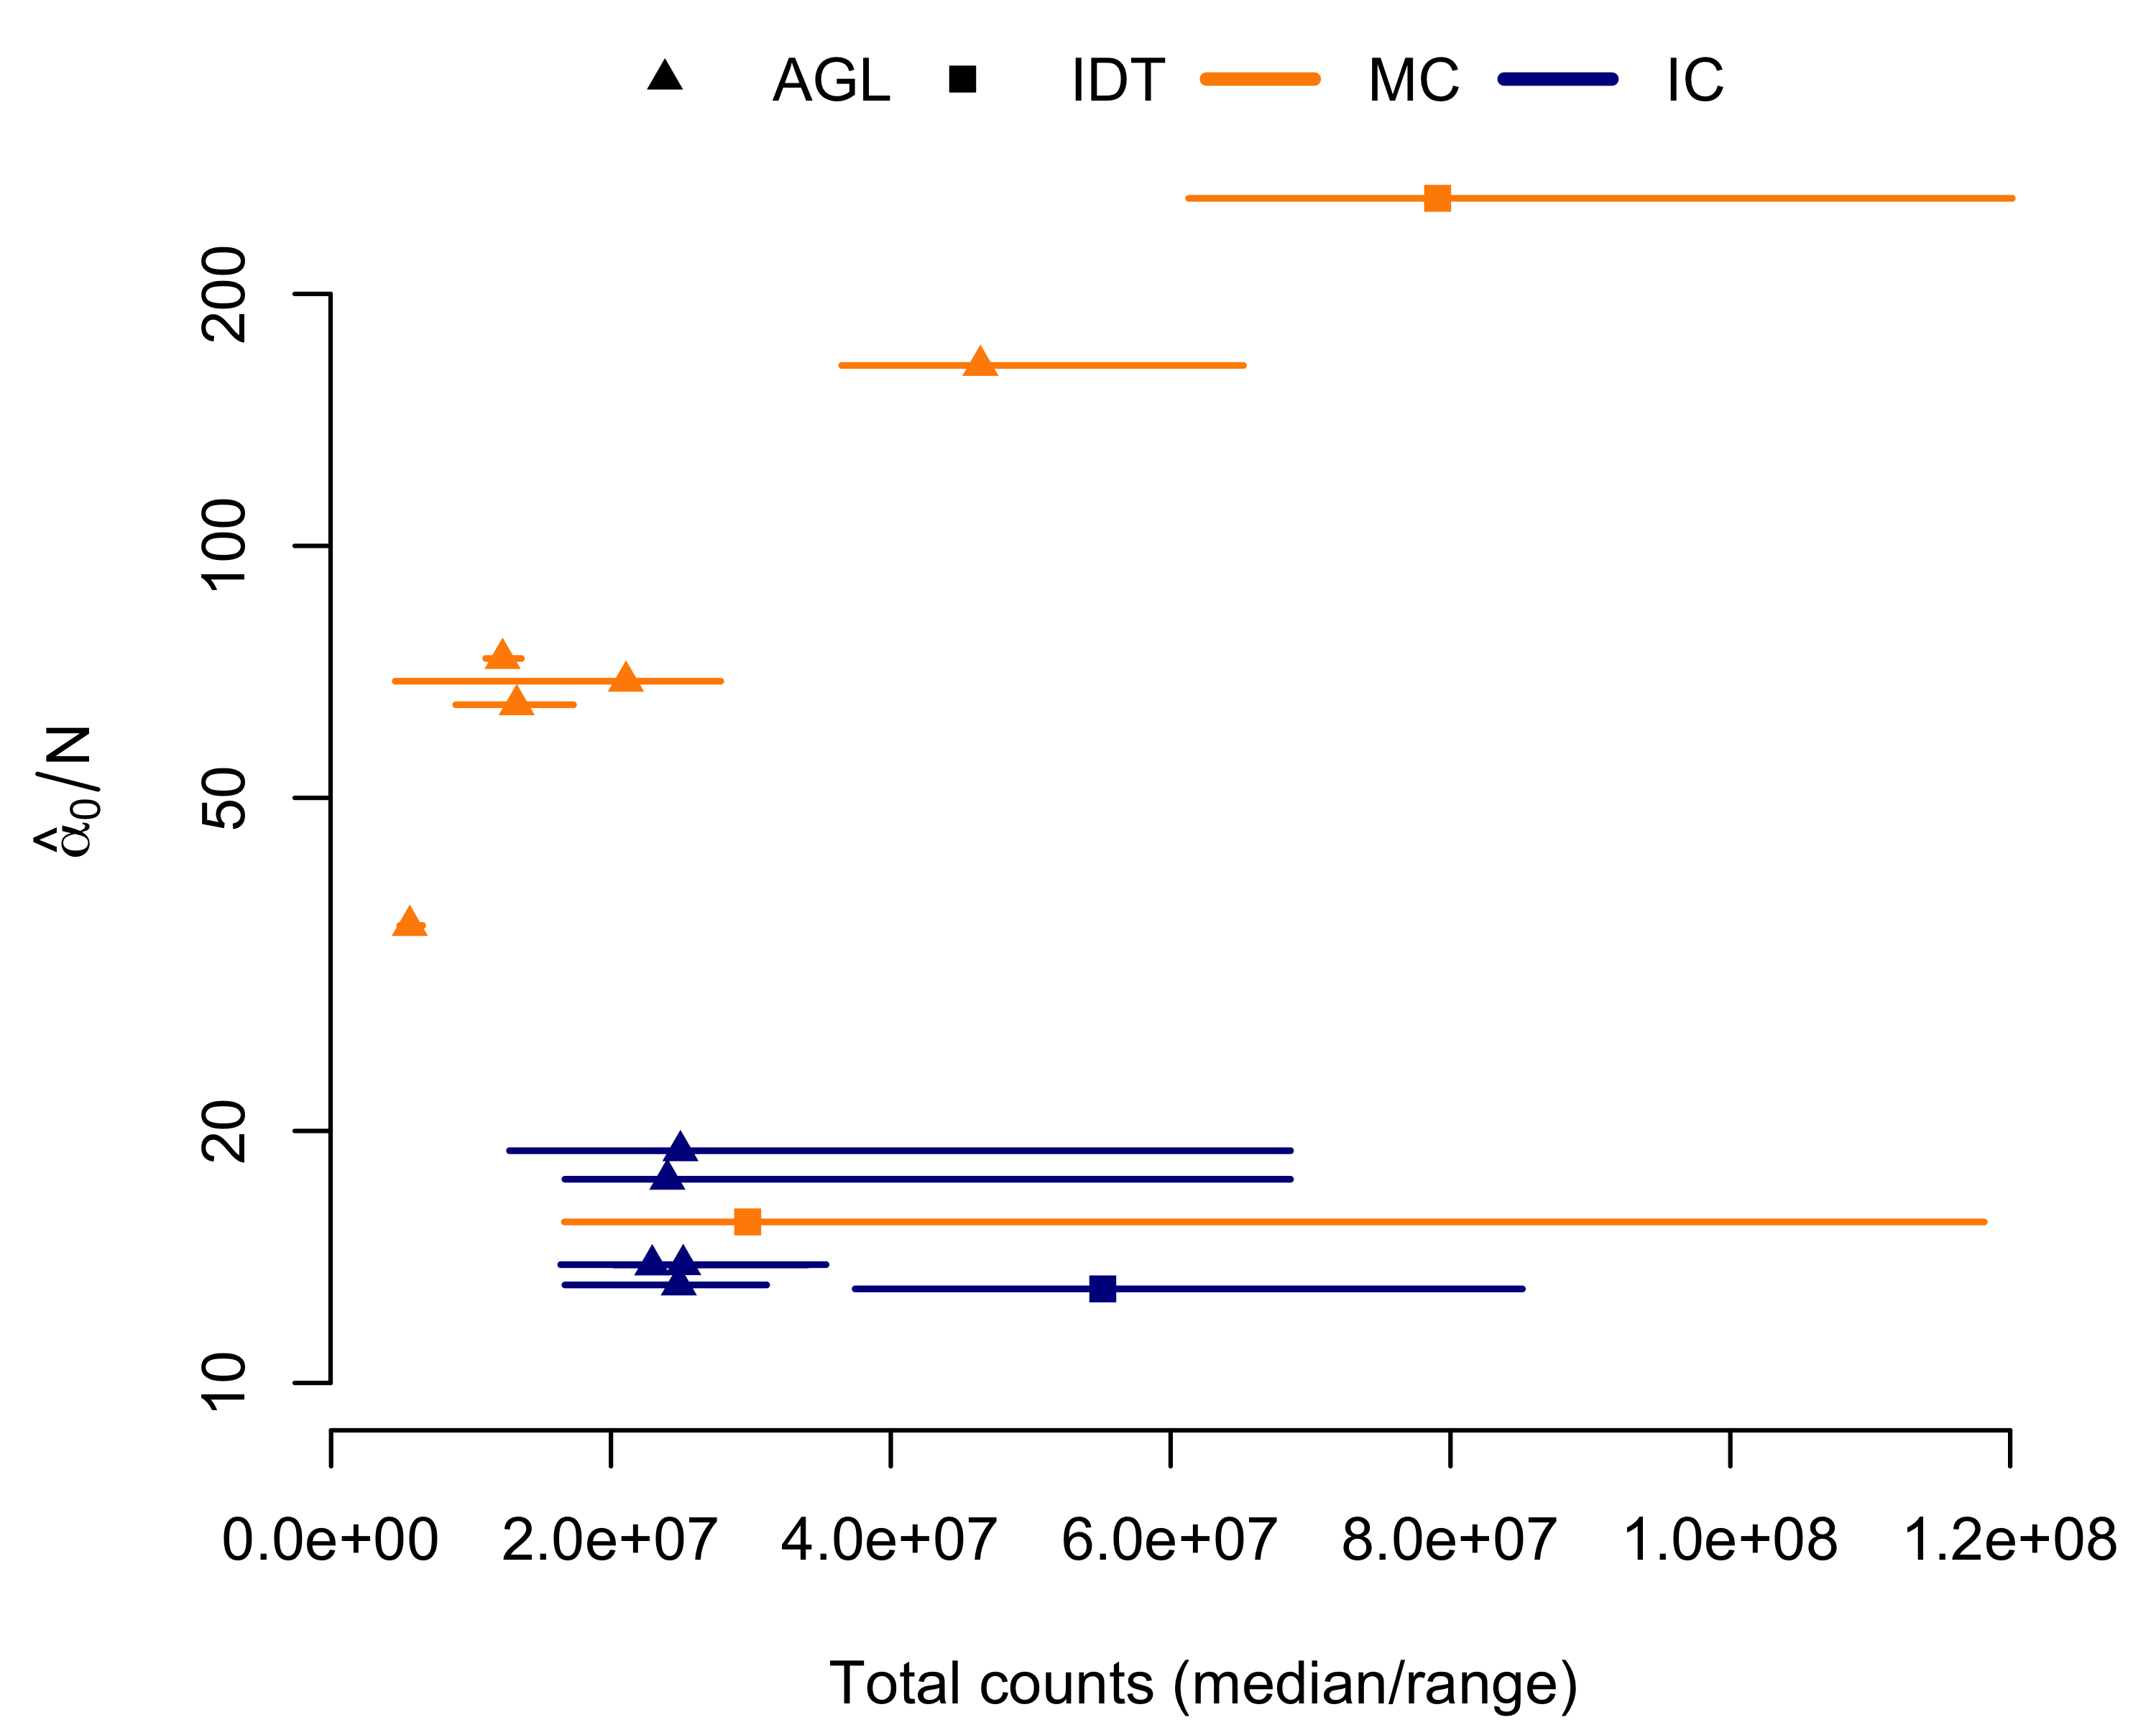
\includegraphics{DLFilerDissertation_files/figure-latex/alpha0-1} 

}

\caption[Multiplexed capture decreases variance with respect to independent captures, as estimated by fitting the dirichlet distribution.]{Multiplexed capture (MC) decreases variance with respect to independent captures (IC), as estimated by fitting the dirichlet distribution. Total counts/sample given on the horizontal axis; mean \(\alpha\) given on the vertical axis. \(\alpha_0\) is inversely proportional to inter-sample variance. Each line/point represents a single pool. The point indicates the median total counts across the pool, with the range given by the line. Orange indicates a multiplexed capture; blue indicates independent captures. Triangles indicate pools using Agilent (AGL) capture; squares indicate Integrated DNA Technologies (IDT).}\label{fig:alpha0}
\end{figure}

The multiplexed pool without decreased inter-sample variance, IDT-MC, had a much larger spread in sequencing depth across the pool (Table \ref{tab:poolSummary}, Figure \ref{fig:alpha0}).
Looking at the total mapped molecules, the IDT-MC pool had a relative standard deviation of 64.2\%, over double the next highest pool.
We hypothesized the absent reduction in variation stemmed from poor library balance during the multiplexing step.
We subsequently captured a new pool using the same DNA input, IDT-RR, and found comparable reductions in inter-sample variance (the pool with the highest \(\alpha_0\) in Figure \ref{fig:alpha0}).

Examining the mean-variance relationship demonstrated the same inter-sample variance reduction suggested by the dirichlet parameter estimates (Figures \ref{fig:mnVrAgl} and \ref{fig:mnVrIdt}).
The Agilent pools (Figure \ref{fig:mnVrAgl}) segregated cleanly, with less dispersion in the multiplexed capture pools.
Again, we found no variance reduction for the IDT-MC pool, overlapping with independently-captured IDT-IC pool (Figure \ref{fig:mnVrAgl}).
We did, however, observe near-complete reduction in dispersion for the better-balanced IDT-RR pool.





\begin{figure}

{\centering 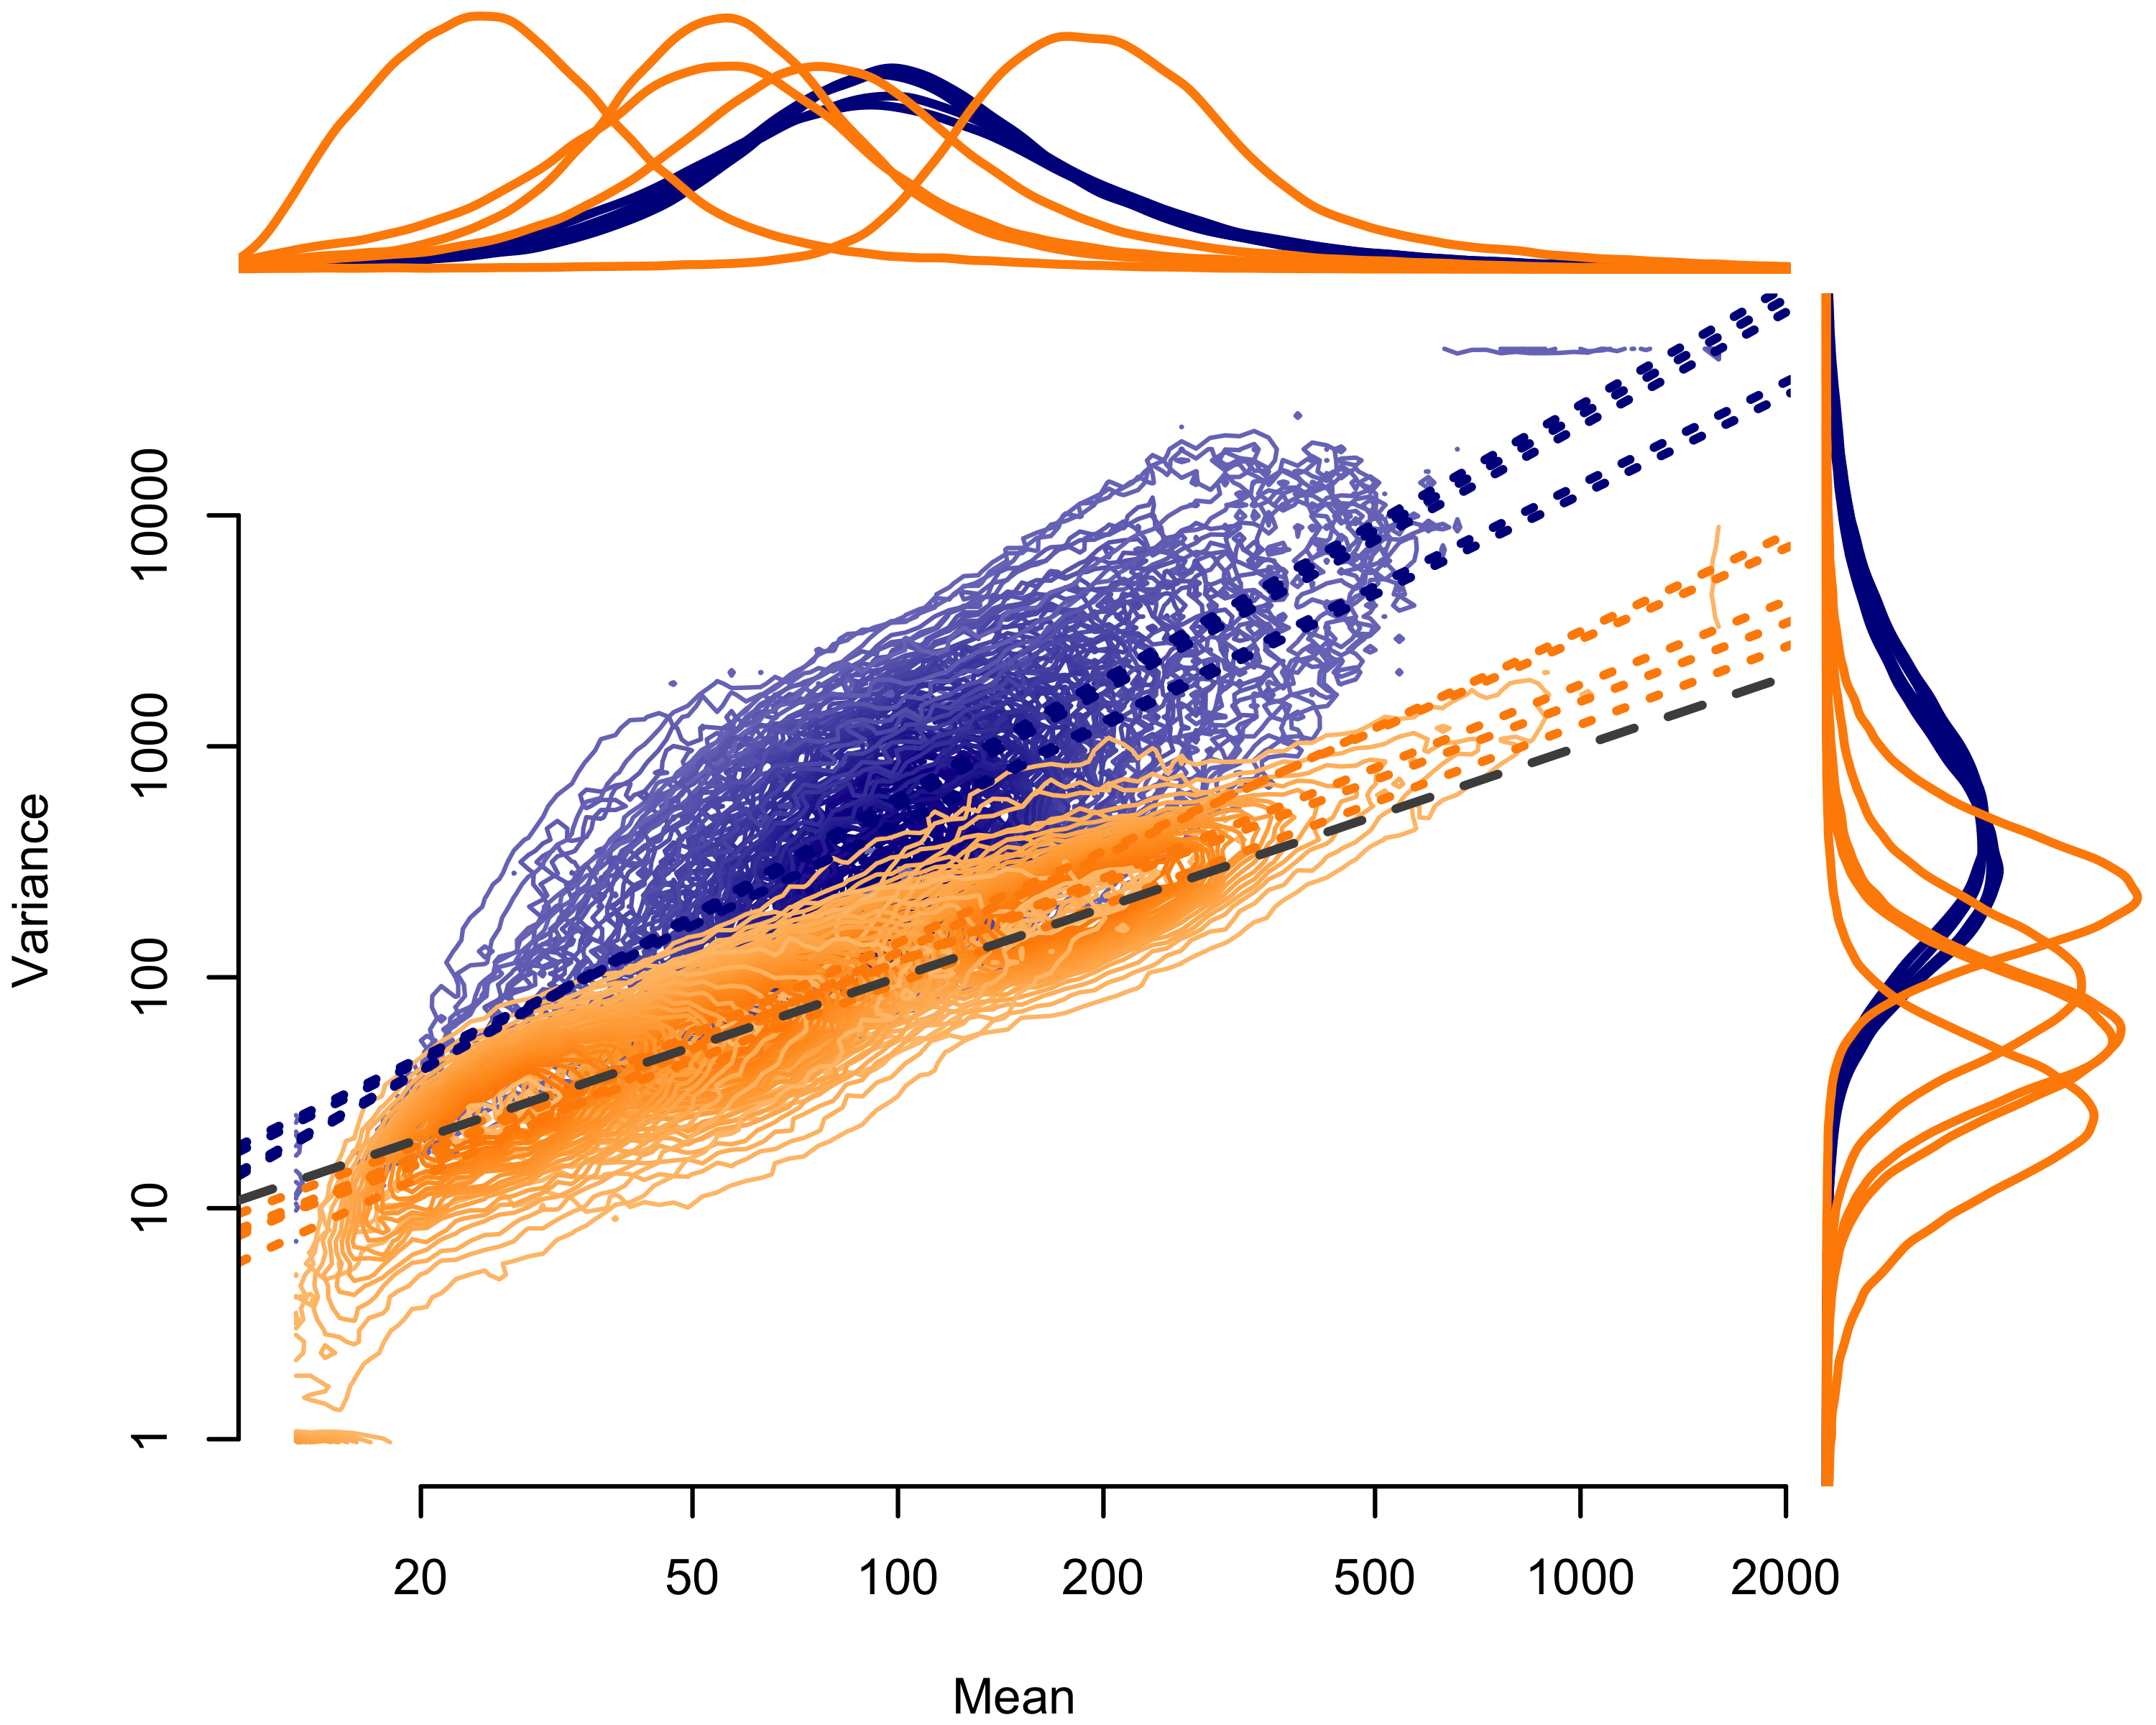
\includegraphics{DLFilerDissertation_files/figure-latex/mnVrAgl-1} 

}

\caption[Mean-variance relationship for Agilent (AGL) pools.]{Mean-variance relationship for Agilent (AGL) pools. Mean counts per exon given on the horizontal axis; mean variance per exon given on the vertical axis. Contours show the distribution of points by pool. Dotted lines show the ordinary least squares regression fit. Orange indicates multiplexed capture pools; blue indicates independently captured pools. The dashed gray line represents the 1:1 relationship expected under a Poisson process. Lines above the plot show the density of mean values by pool; lines to the right of the plot show the density of variance values by pool.}\label{fig:mnVrAgl}
\end{figure}



\begin{figure}

{\centering 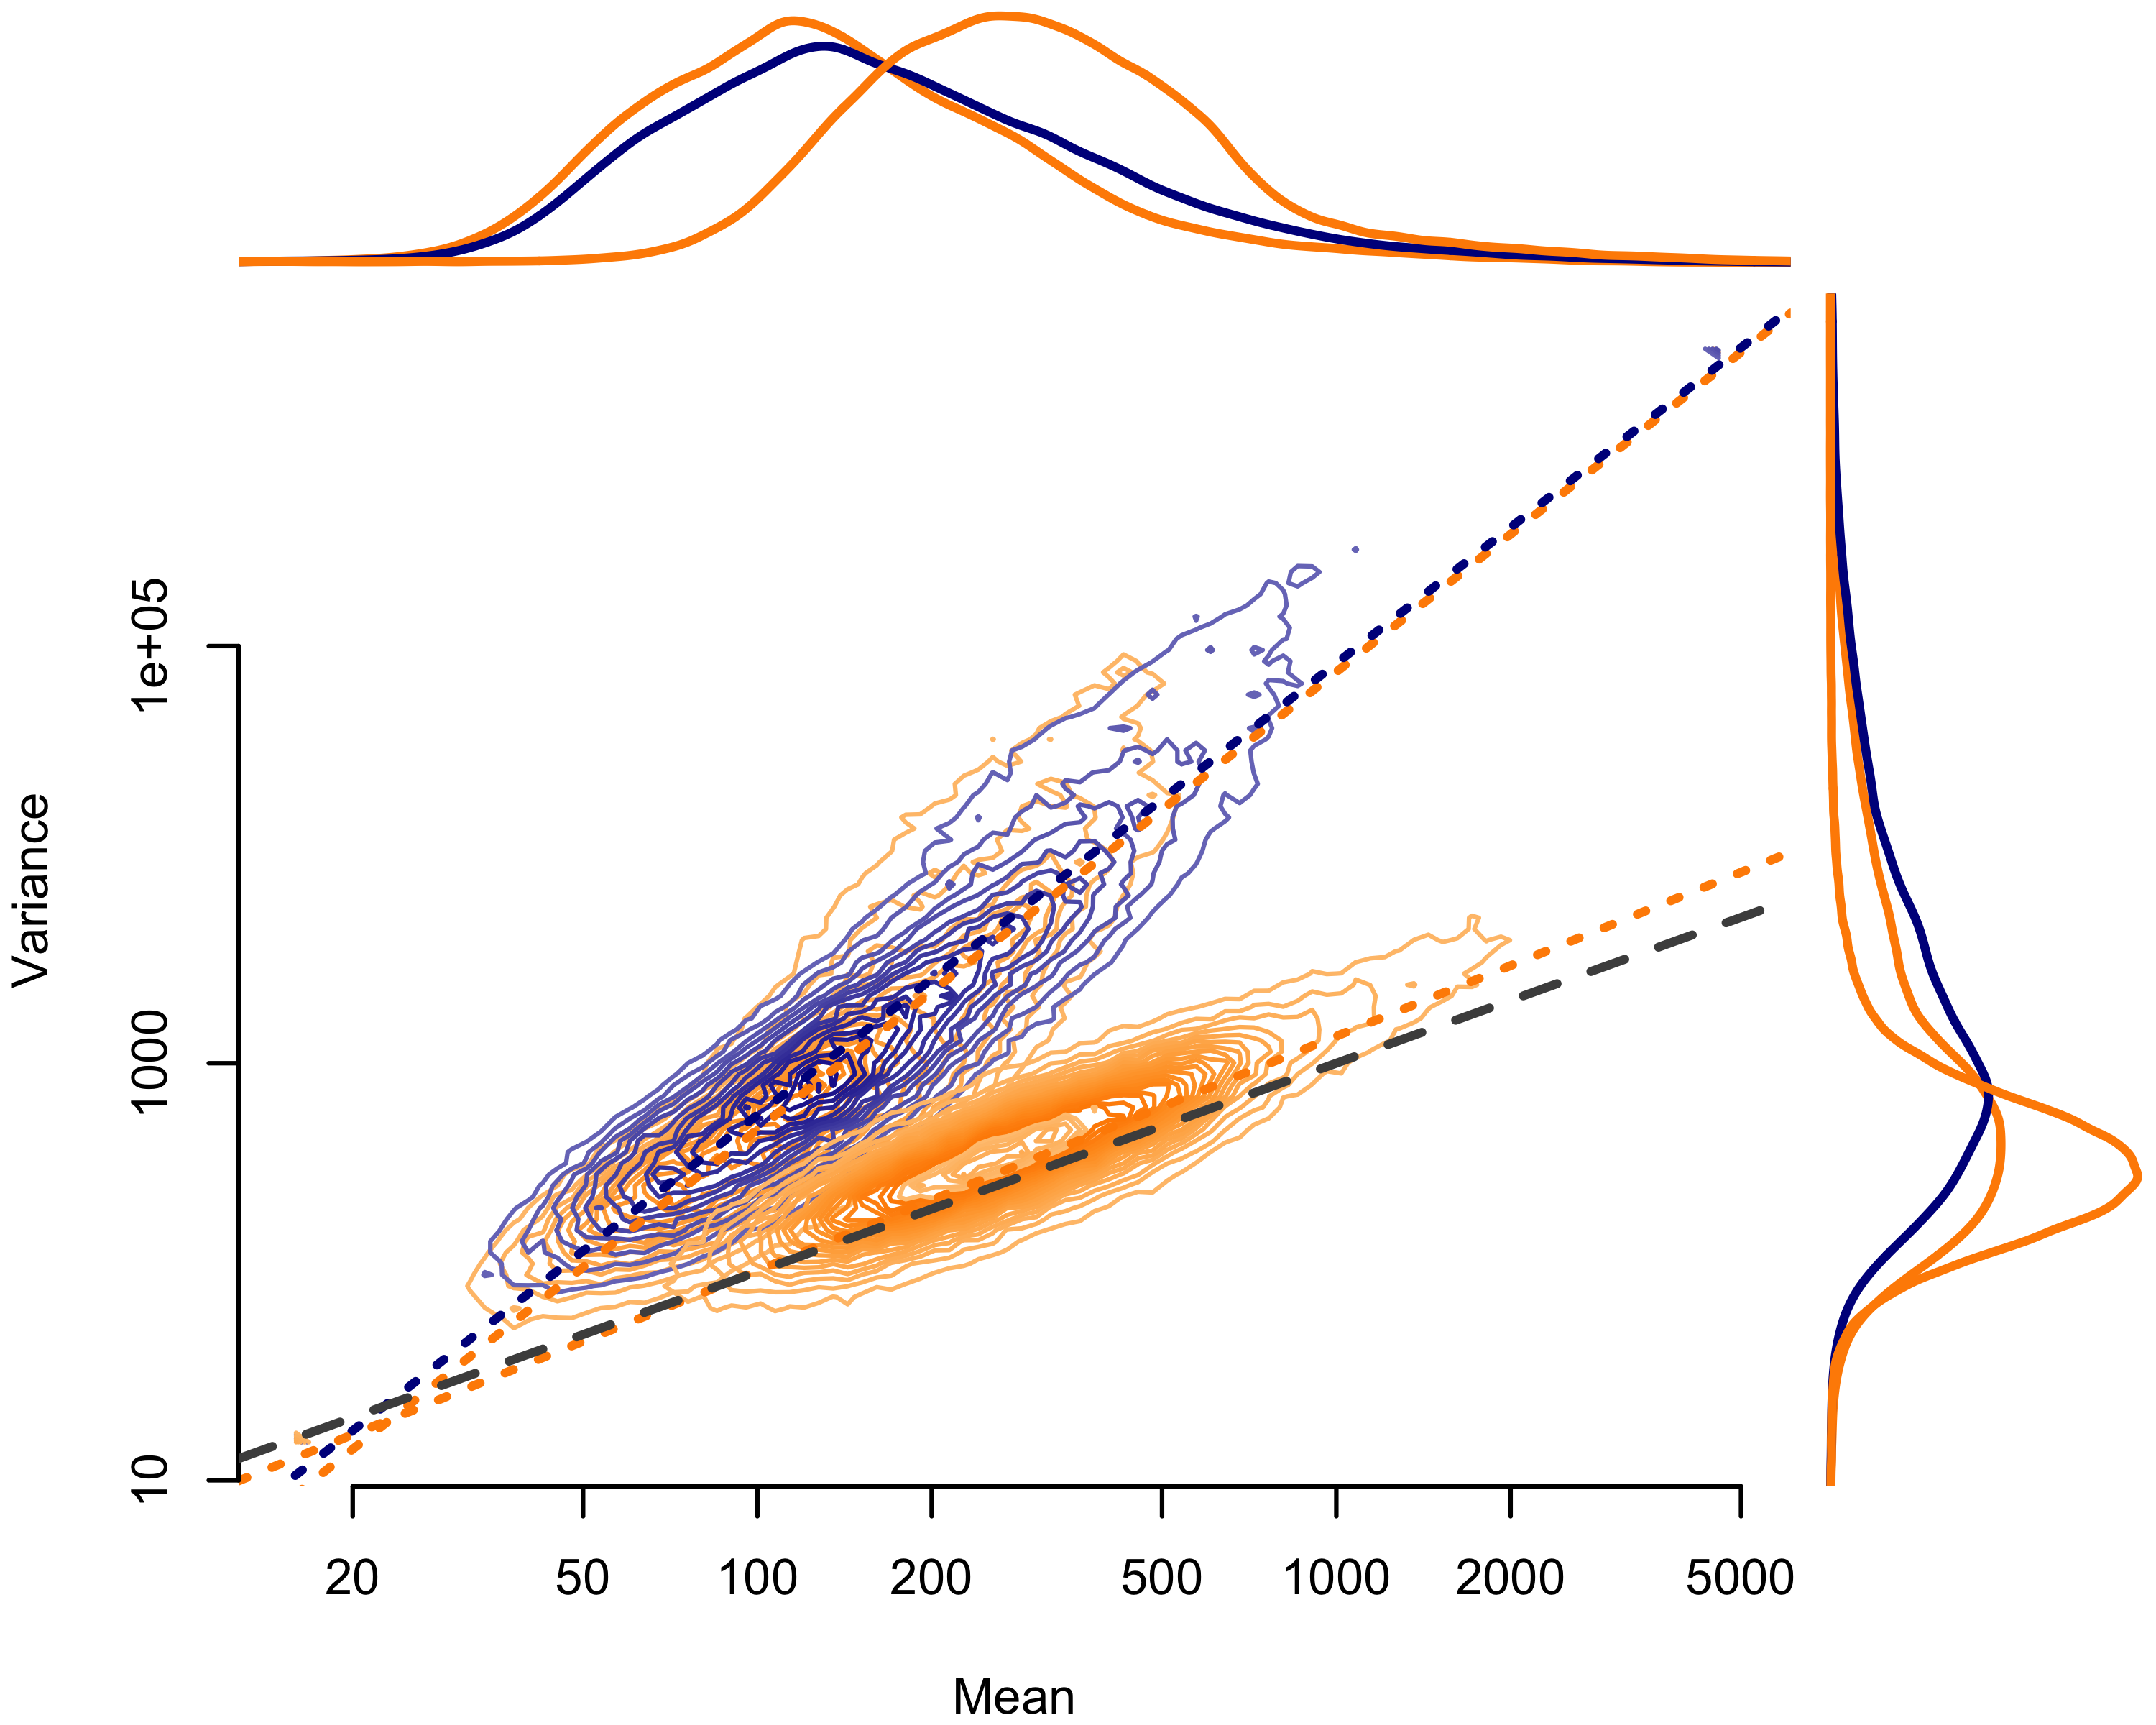
\includegraphics{DLFilerDissertation_files/figure-latex/mnVrIdt-1} 

}

\caption[Mean-variance relationship for Integrated DNA Technologies (IDT) pools.]{Mean-variance relationship for Integrated DNA Technologies (IDT) pools. Mean counts per exon given on the horizontal axis; mean variance per exon given on the vertical axis. Contours show the distribution of points by pool. Dotted lines show the ordinary least squares regression fit. Orange indicates multiplexed capture pools; blue indicates independently captured pools. The dashed gray line represents the 1:1 relationship expected under a Poisson process. Lines above the plot show the density of mean values by pool; lines to the right of the plot show the density of variance values by pool.}\label{fig:mnVrIdt}
\end{figure}





\begin{figure}

{\centering 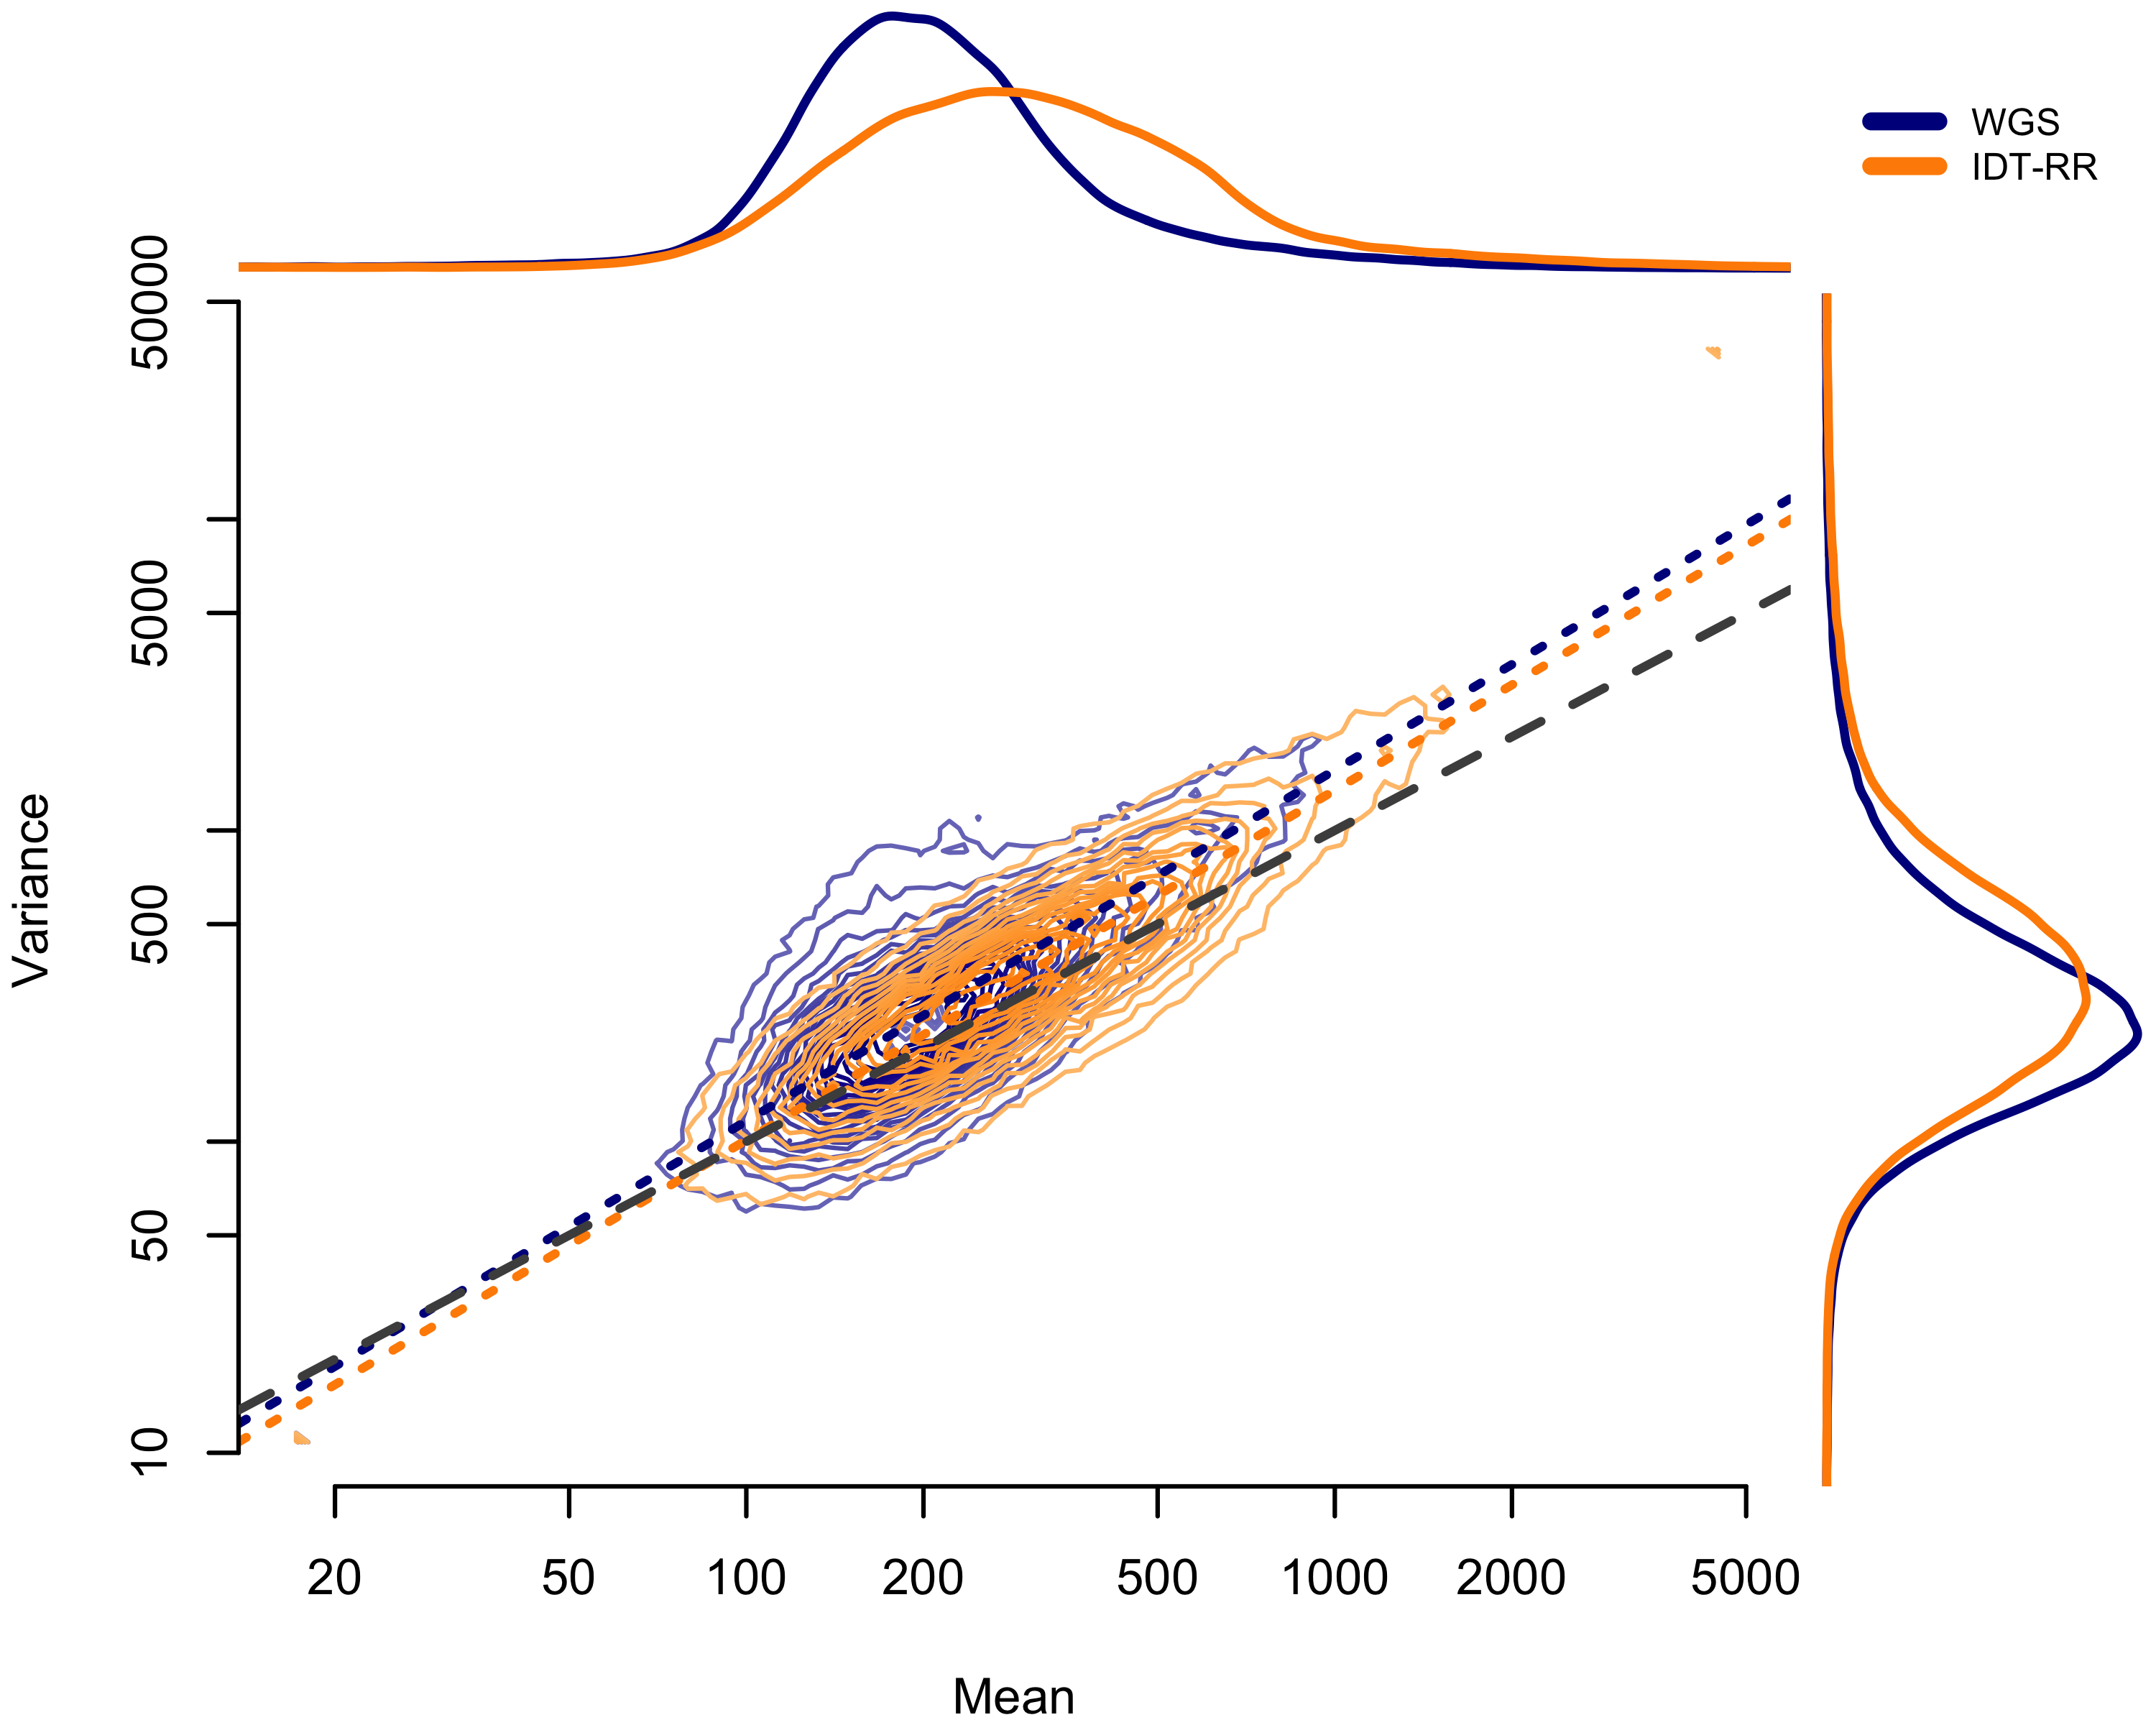
\includegraphics{DLFilerDissertation_files/figure-latex/mnVrComp-1} 

}

\caption[Comparison of mean-variance relationship between WGS pool and IDT-RR pool.]{Comparison of mean-variance relationship between WGS pool (blue) and IDT-RR pool (orange). Mean count by exon given on horizontal axis; variance of exon counts given on horizontal axis. Dotted lines show the ordinary least-squares fit. Lines above plot show the distribution of mean values; lines to the right of the plot show the distribution of variance values.}\label{fig:mnVrComp}
\end{figure}

\hypertarget{multiplexed-capture-provides-controls-for-exomedepth}{%
\subsection{Multiplexed capture provides controls for ExomeDepth}\label{multiplexed-capture-provides-controls-for-exomedepth}}

ExomeDepth requires a set of control subjects, summed into a reference vector of counts at each exon.
ExomeDepth provides functionality to select appropriate controls from a set of subjects, often requiring large numbers of subjects to identify appropriate controls.
Smaller research groups and clinical laboratories may struggle building large databases of exomes, with the difficulty compounded by lot-to-lot variation and regular improvements to capture and sequencing chemistries.
We wanted to know if the reduced inter-sample variance with multiplexed capture could provide an appropriate control set for ExomeDepth, eliminating the need for large databases of similarly-captured exomes.
We found the reduced inter-sample variance with multiplexed capture leads to appropriate control selection for ExomeDepth (Figures \ref{fig:edSelMed}).
Pool2, where we repeated the initial fragmentation 5 times, did not perform as well as the other multiplexed pools.
We also found two samples within the WGS pool did not correlate well with the rest of the pool.





\begin{figure}

{\centering 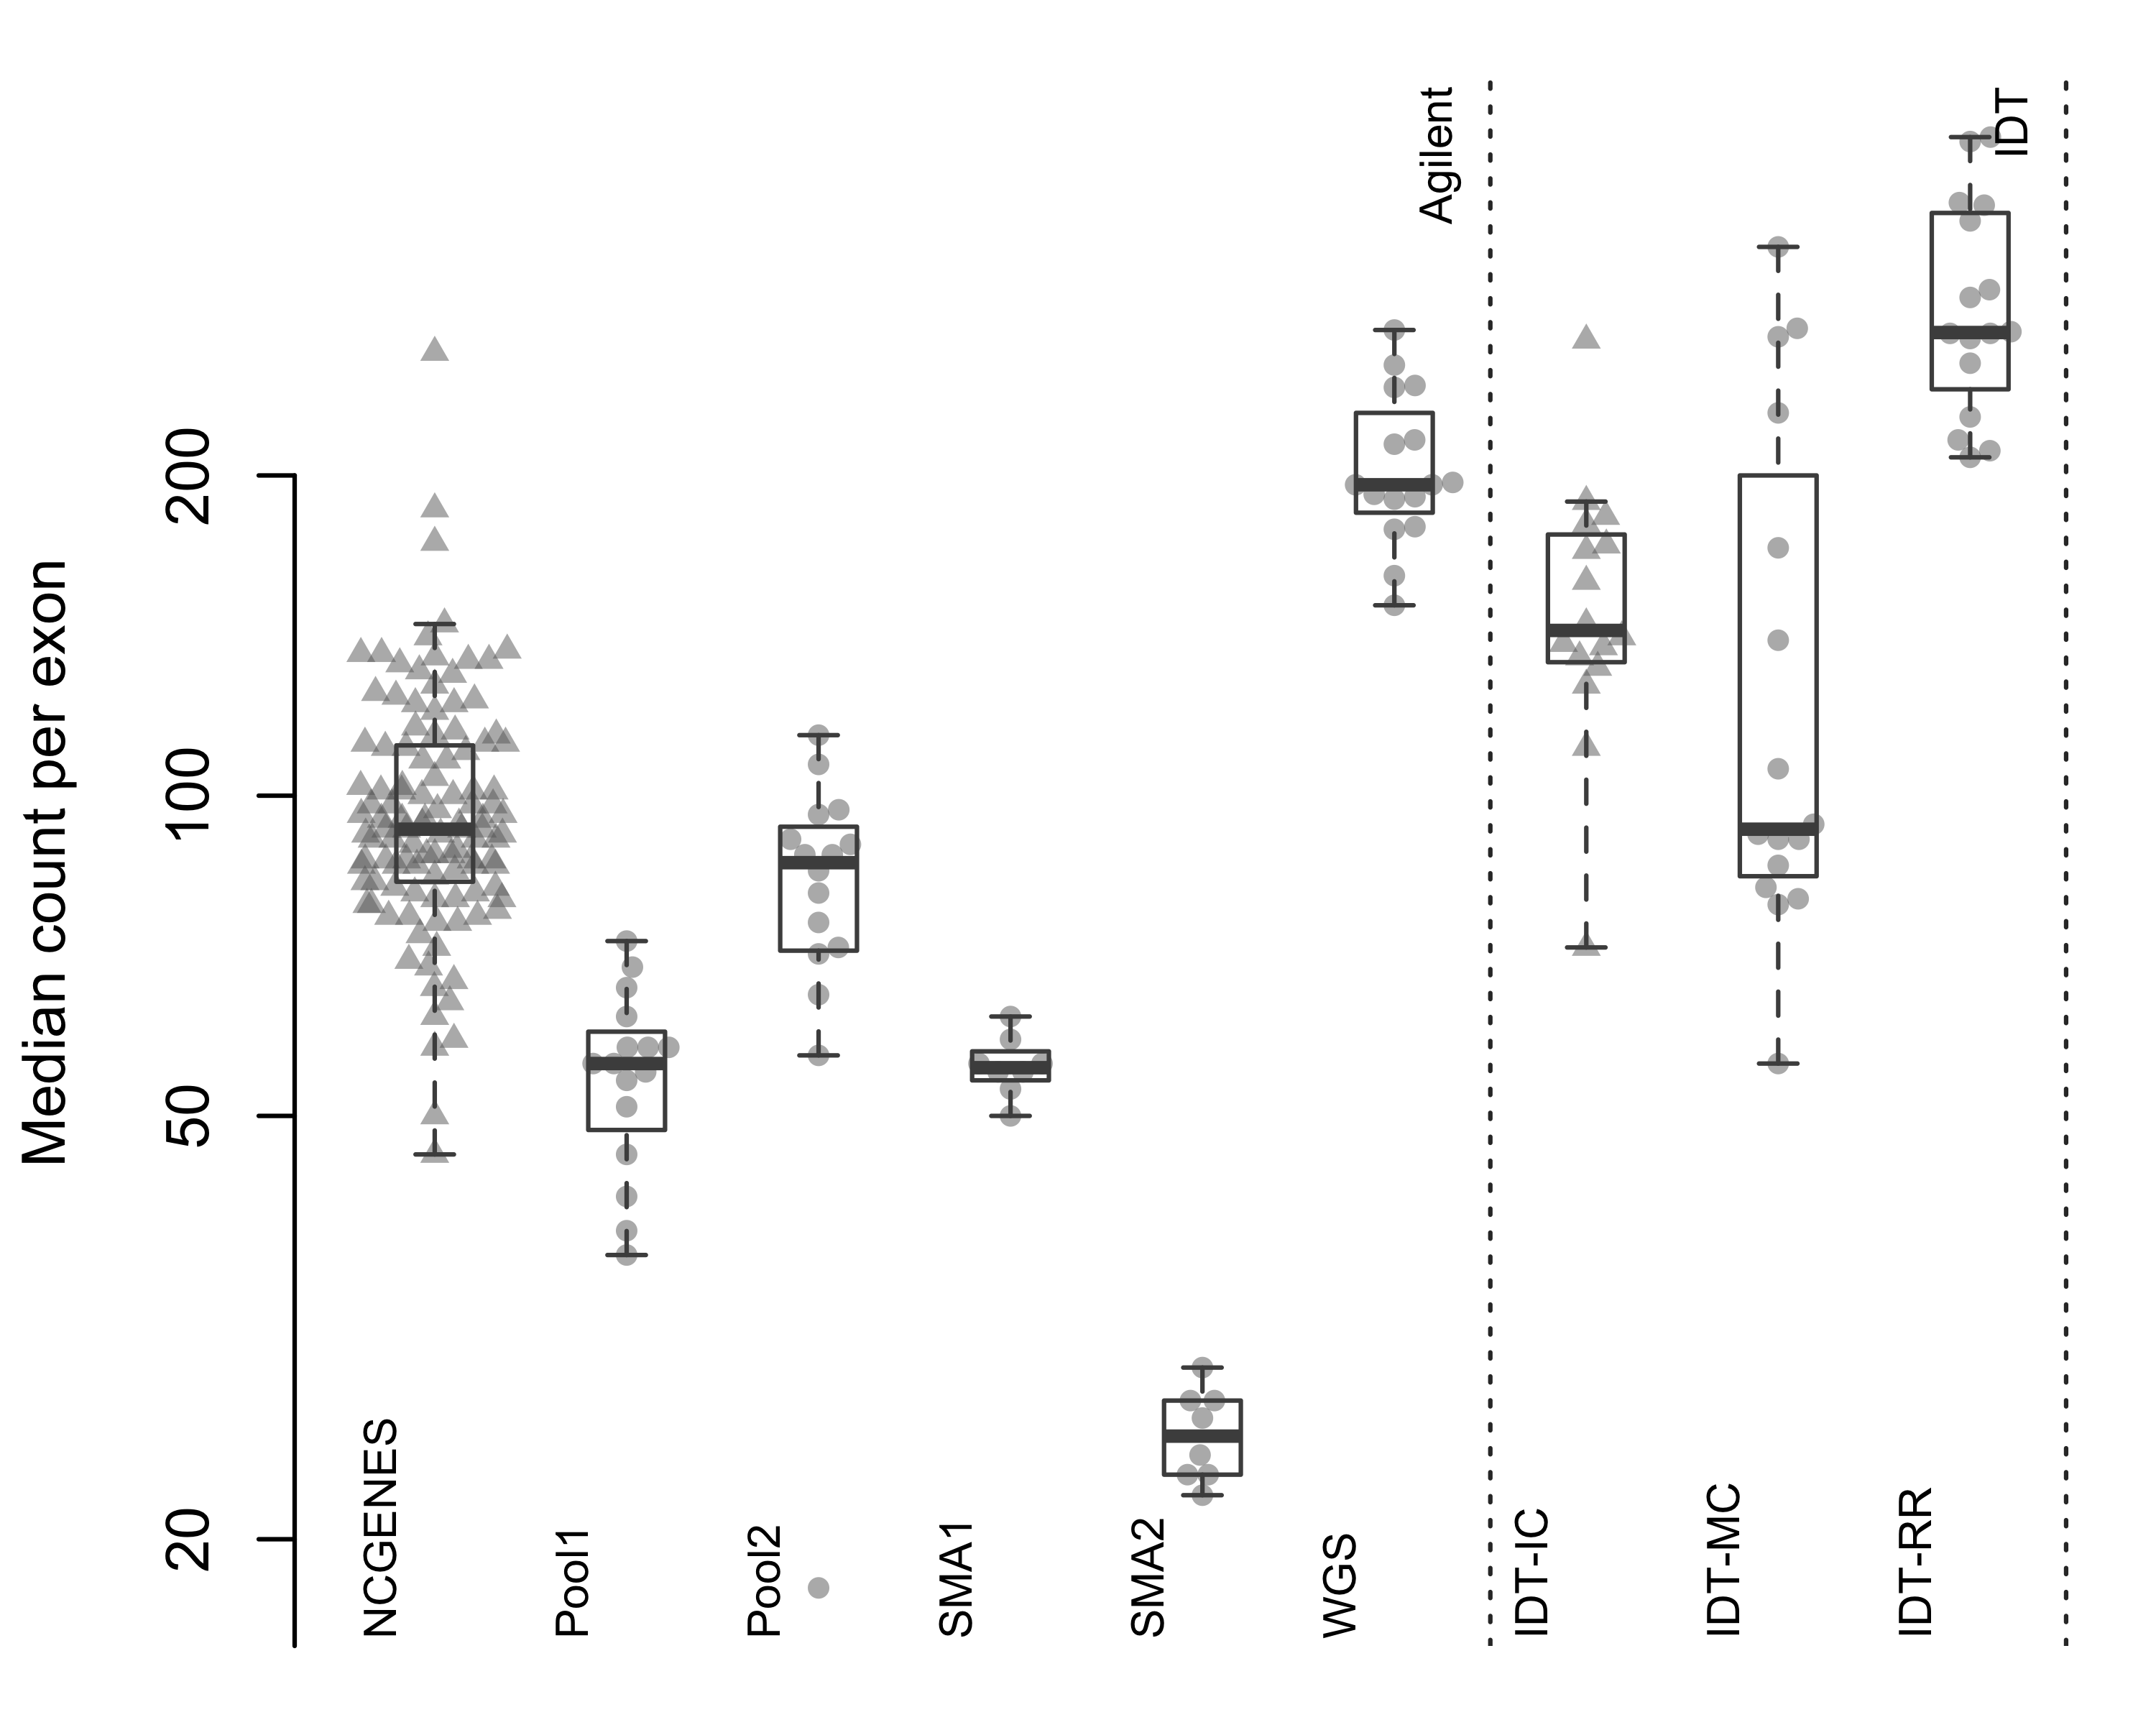
\includegraphics{DLFilerDissertation_files/figure-latex/edSelMed-1} 

}

\caption[Median count per exon.]{Median count per exon. Each point represents a single sample, with samples grouped by pool. Triangles indicate independently-captured samples; circles indiciate a single multiplexed capture within the pool. Dotted vertical line separates the two capture platforms.}\label{fig:edSelMed}
\end{figure}



\begin{figure}

{\centering 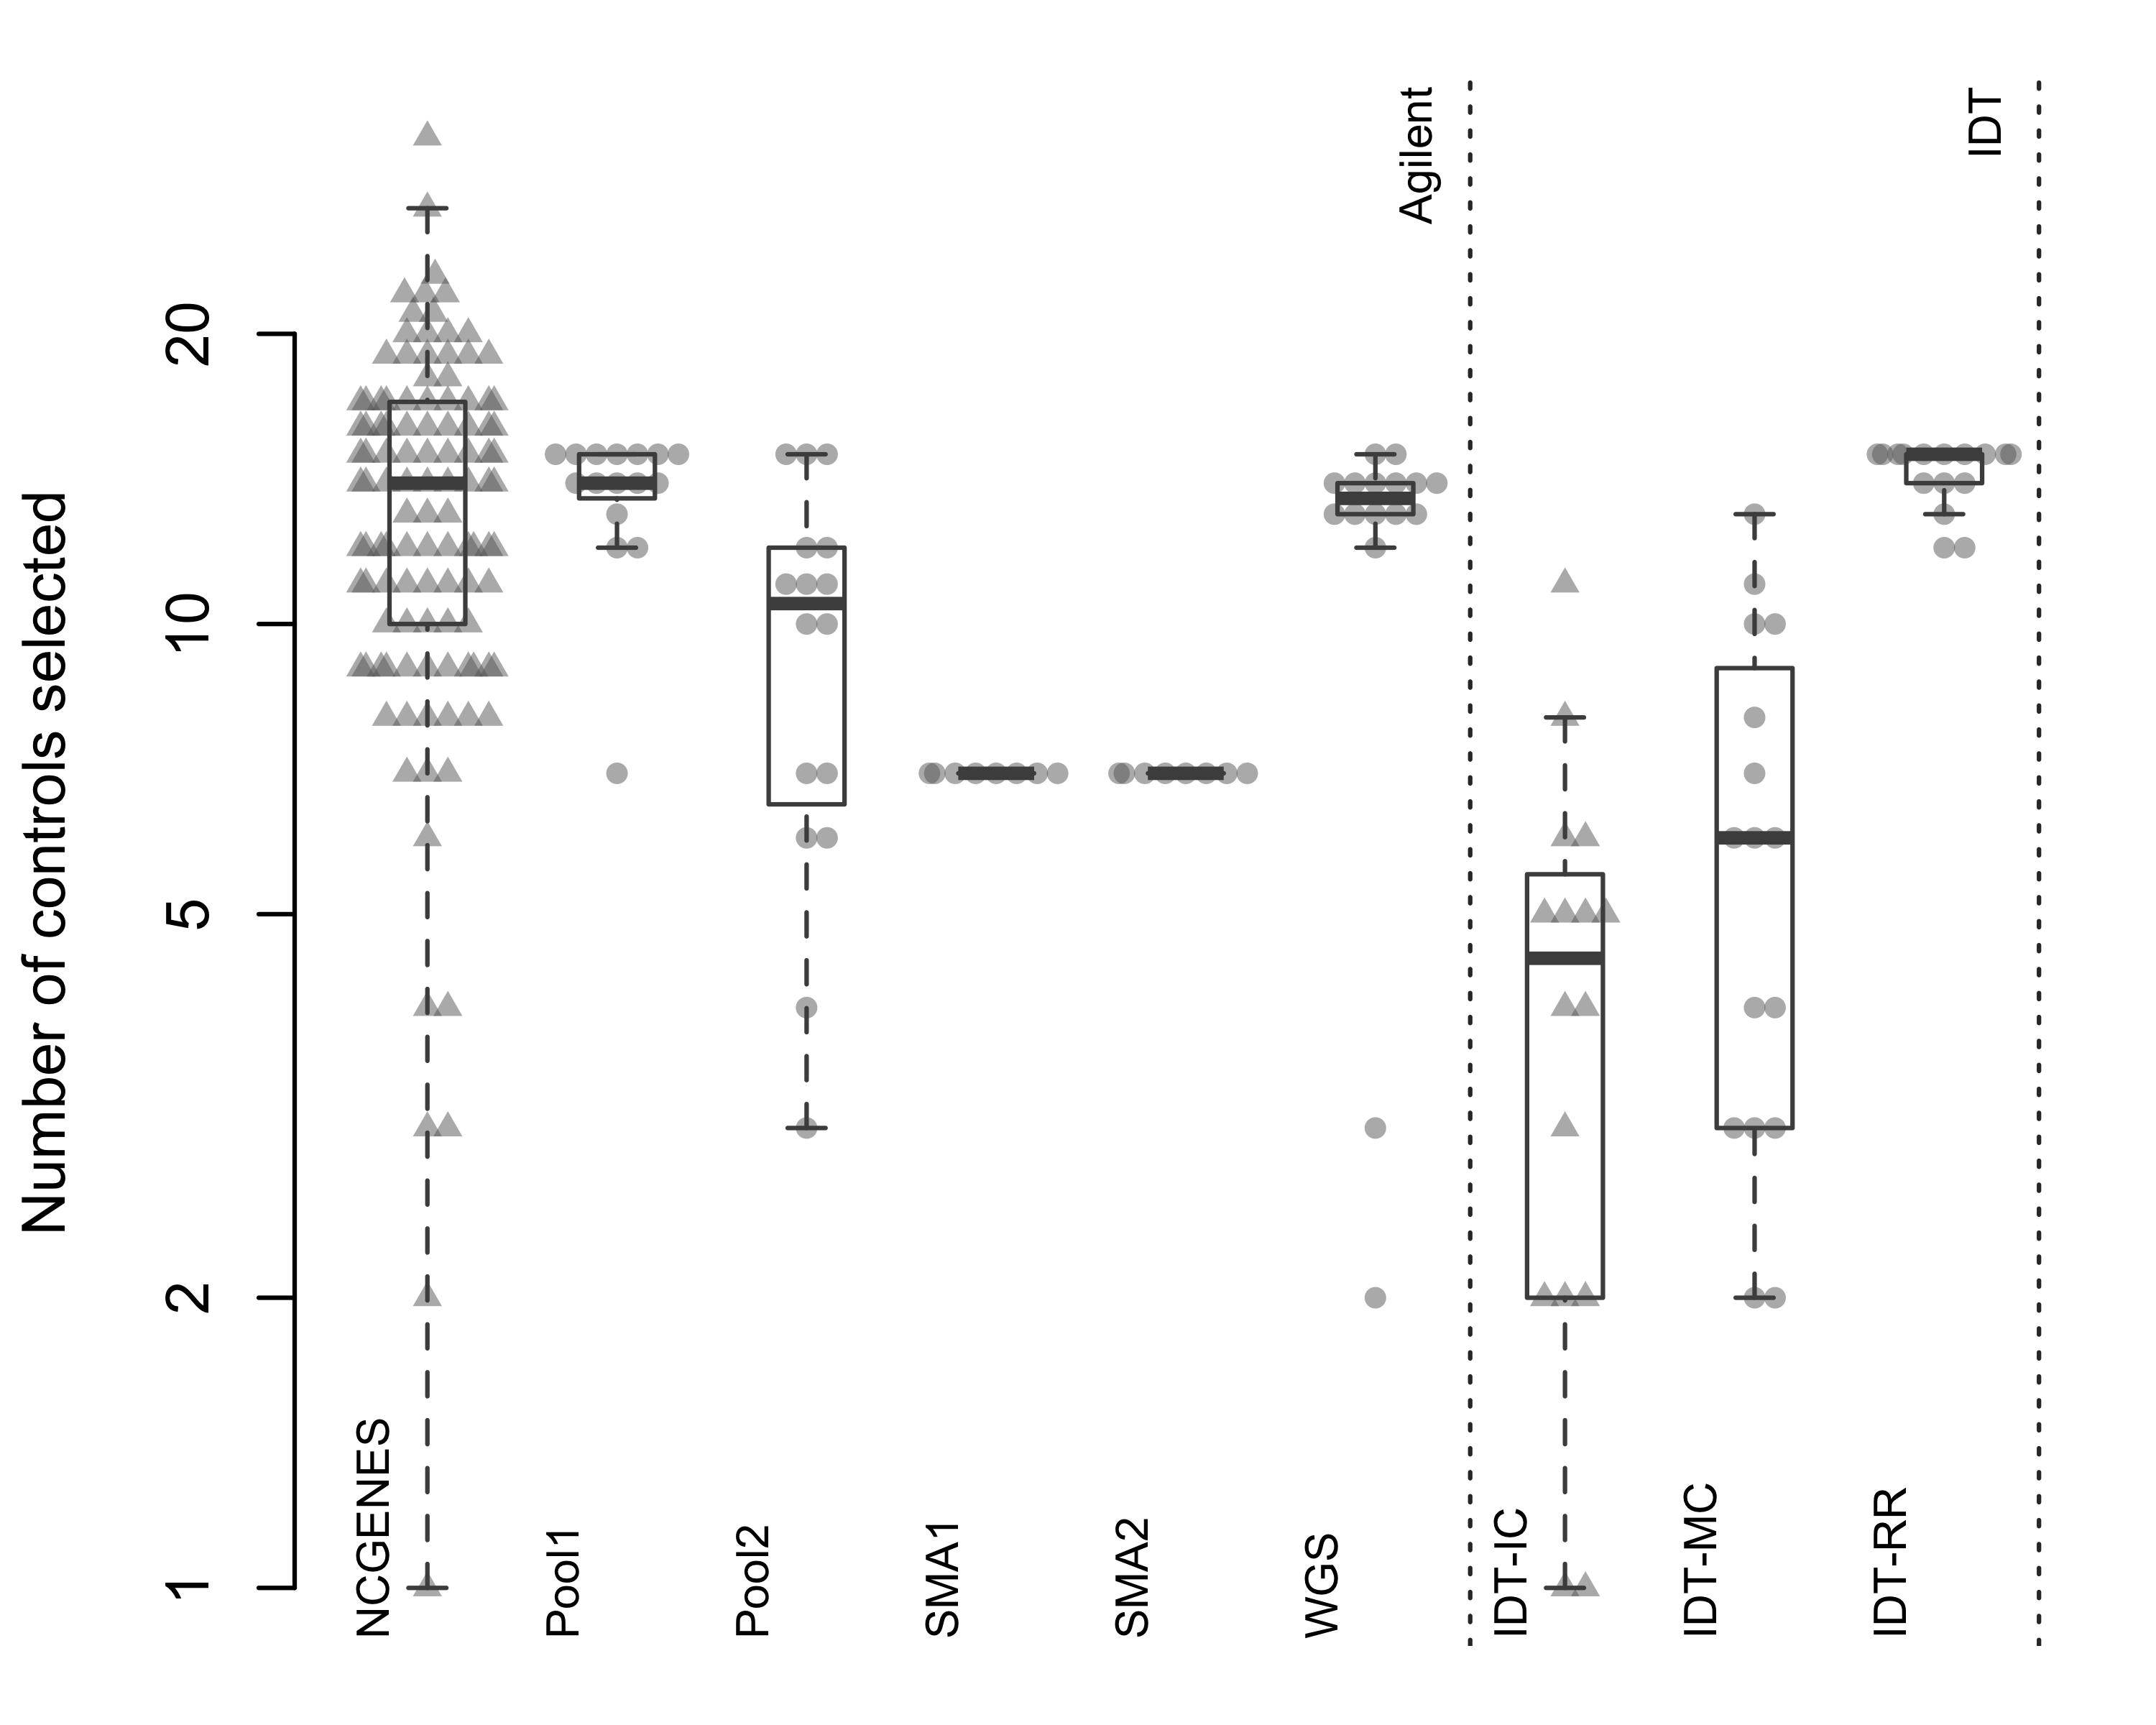
\includegraphics{DLFilerDissertation_files/figure-latex/edSelTot-1} 

}

\caption[Total number of controls selected by ExomeDepth.]{Total number of controls selected by ExomeDepth. Each point represents a single sample, with samples grouped by pool. Triangles indicate independently-captured samples; circles indiciate a single multiplexed capture within the pool. Dotted vertical line separates the two capture platforms.}\label{fig:edSelTot}
\end{figure}



\begin{figure}

{\centering 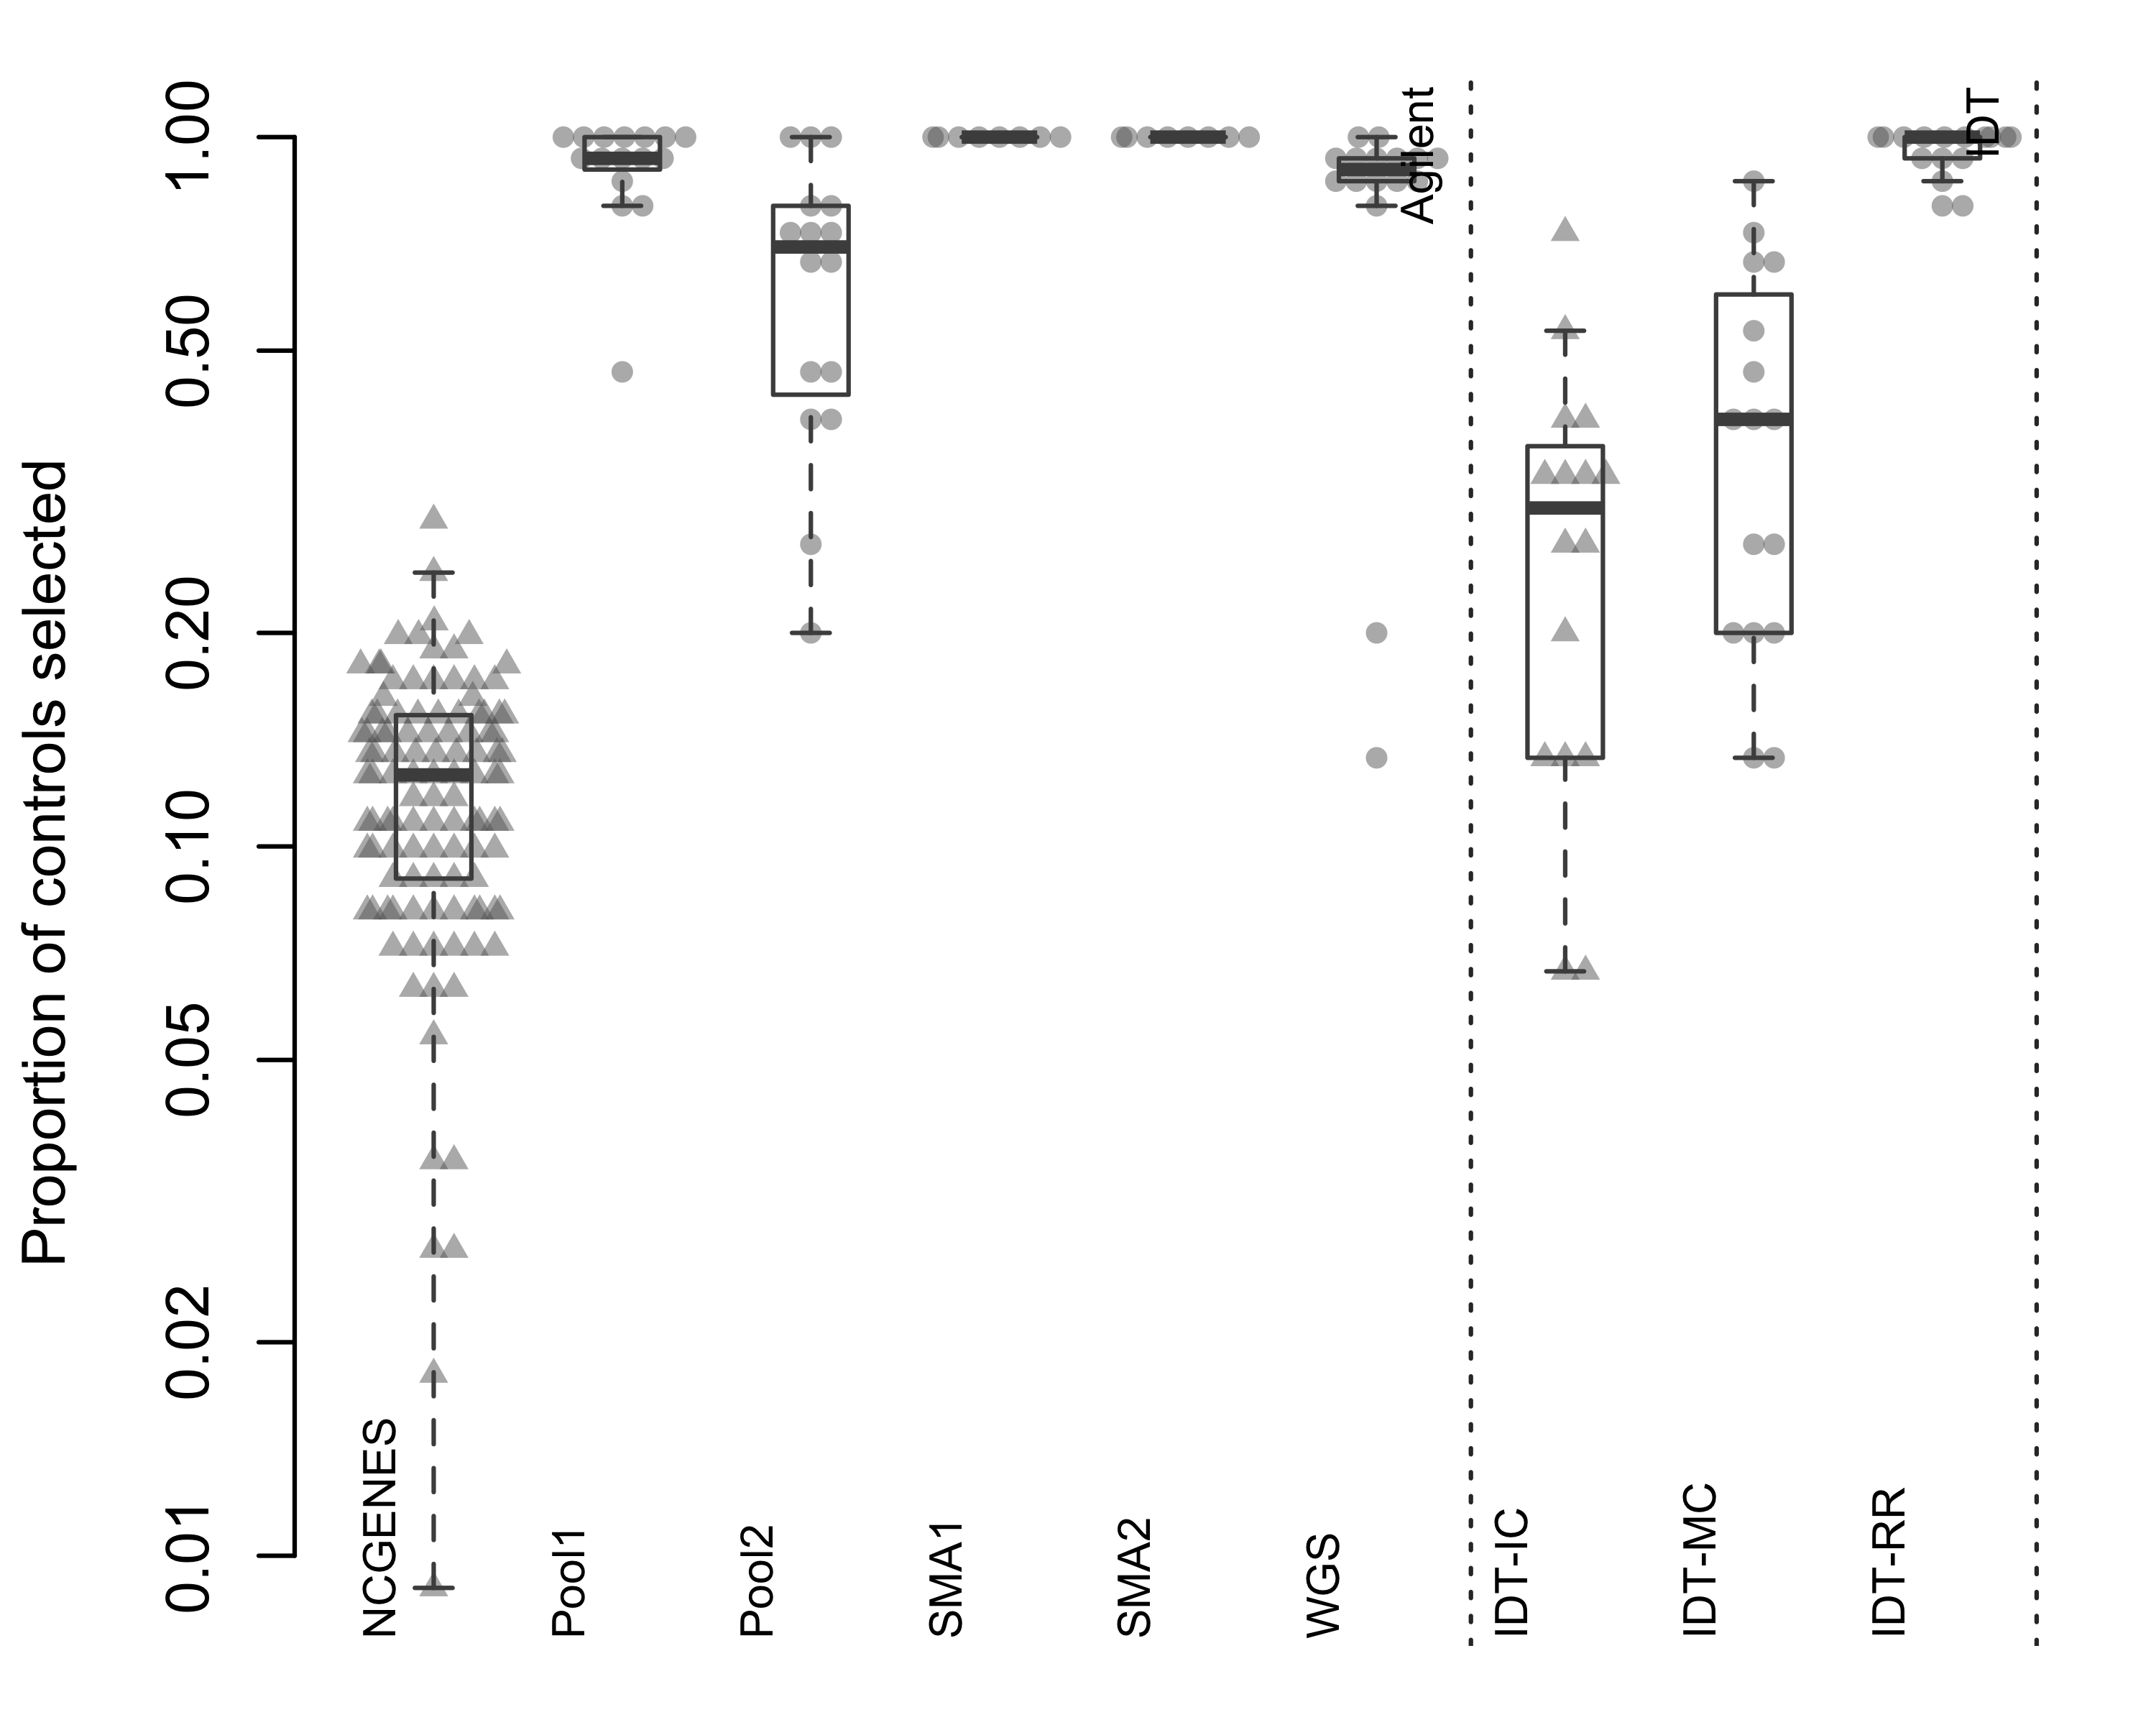
\includegraphics{DLFilerDissertation_files/figure-latex/edSelProp-1} 

}

\caption[Proportion of available samples selected by ExomeDepth as a control.]{Proportion of available samples selected by ExomeDepth as a control. Each point represents a single sample, with samples grouped by pool. Triangles indicate independently-captured samples; circles indiciate a single multiplexed capture within the pool. Dotted vertical line separates the two capture platforms.}\label{fig:edSelProp}
\end{figure}



\begin{figure}

{\centering 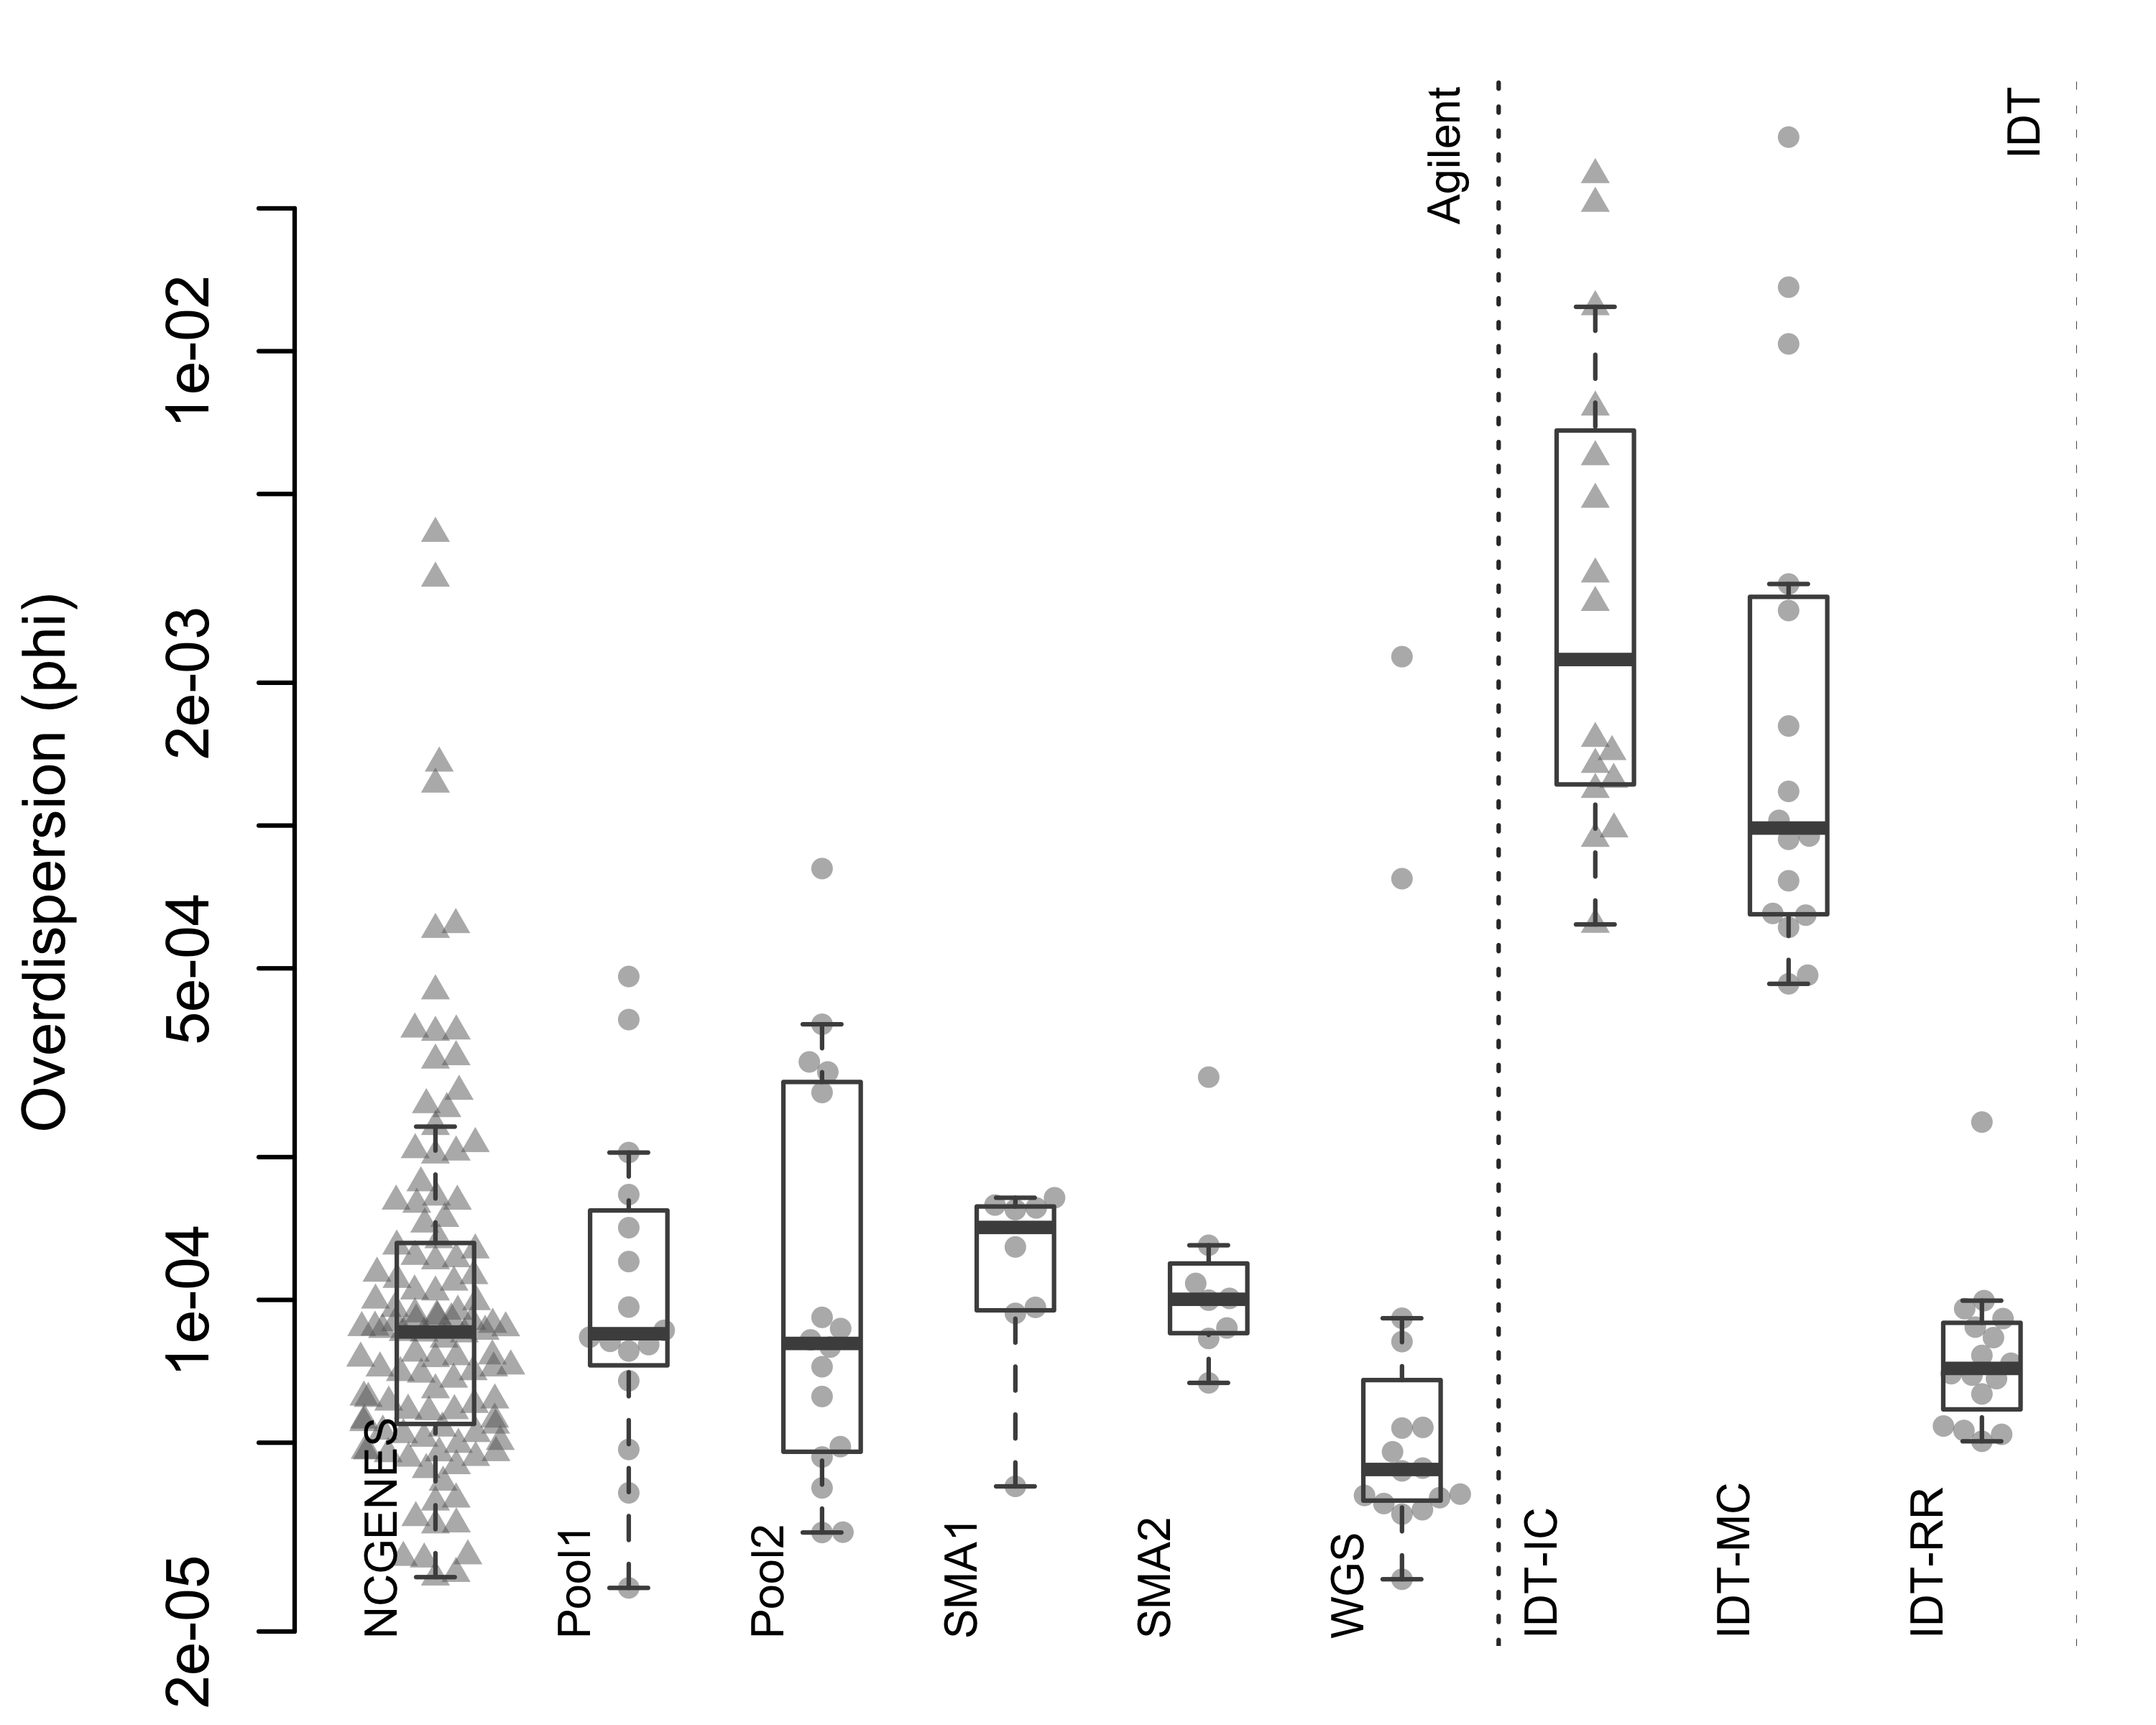
\includegraphics{DLFilerDissertation_files/figure-latex/edSelPhi-1} 

}

\caption[Estimated phi parameter from ExomeDepth.]{Estimated phi parameter from ExomeDepth. Each point represents a single sample, with samples grouped by pool. Triangles indicate independently-captured samples; circles indiciate a single multiplexed capture within the pool. Dotted vertical line separates the two capture platforms.}\label{fig:edSelPhi}
\end{figure}

When we looked at independently-captured subjects, we found appropriate control sets for most of the 112 NCGENES subjects (Figure \ref{fig:edSelTot}).
However, ExomeDepth only selected 12.2\% of available samples as controls, on average (Figure \ref{fig:edSelProp}).
Similarly, with the independently-captured IDT-IC pool we find low control numbers for most samples.
While possible to select the same number of controls but exhibit differing dispersion, we observed little difference in the dispersion between independent and multiplexed capture (Figure \ref{fig:edSelPhi}).
Overall, multiplexed capture provided appropriate controls for most samples tested, however an adequately-large set of available controls delivered comparable performance.

\hypertarget{mccnv-exomedepth-perform-comparably-in-simulation-study}{%
\subsection{mcCNV \& ExomeDepth perform comparably in simulation study}\label{mccnv-exomedepth-perform-comparably-in-simulation-study}}

To compare our mcCNV algorithm and ExomeDepth, we created synthetic pools of data across different sequencing depths.
Based on our observations with the real data, we selected the total number of molecules for each sample from a uniform distribution defined as a 30\% window on either side of the specified depth; for example, for a specified depth of 10 million molecules, we drew the molecules per sample from 7 to 13 million molecules.
For each depth ranging from 5 to 100 million molecules, we simulated 200 16-sample pools with single-exon variants.
We allowed for homozygous and heterozygous deletions and duplications (0 to 4 copies), such that all variants were equally likely and the total variant probability was \(1/1,000\).
We used, as the starting capture probabilities (\(\mathbb{E}\)), the empiric capture probabilities observed by summing across the Pool1 pool.

We analyzed each of the 4,000 pools (200 replicates by 20 depths) using our algorithm and two iterations of ExomeDepth.
For the first iteration of ExomeDepth, we used the default values for transition probability (\(1/10,000\)) and expected variant length (50 kb).
For the second iteration, we used the true simulated variant prior for the transition probability (\(1/1,000\)) and an expected variant length of 1 kb.
As expected, the sensitivity increased and false discovery rate decreased as the sequencing depth increased (Figures \ref{fig:simRes}).
In both comparisons, mcCNV demonstrated a superior false-discovery rate.
When interrogating Matthew's correlation coefficient\textsuperscript{\protect\hyperlink{ref-matthews:1975aa}{102}} and the sensitivity, we found mcCNV had marginal performance over ExomeDepth with default parameters and marginal performance under ExomeDepth with simulation-matched parameters. Table \ref{tab:simResTbl} provides the actual values.





\begin{figure}

{\centering 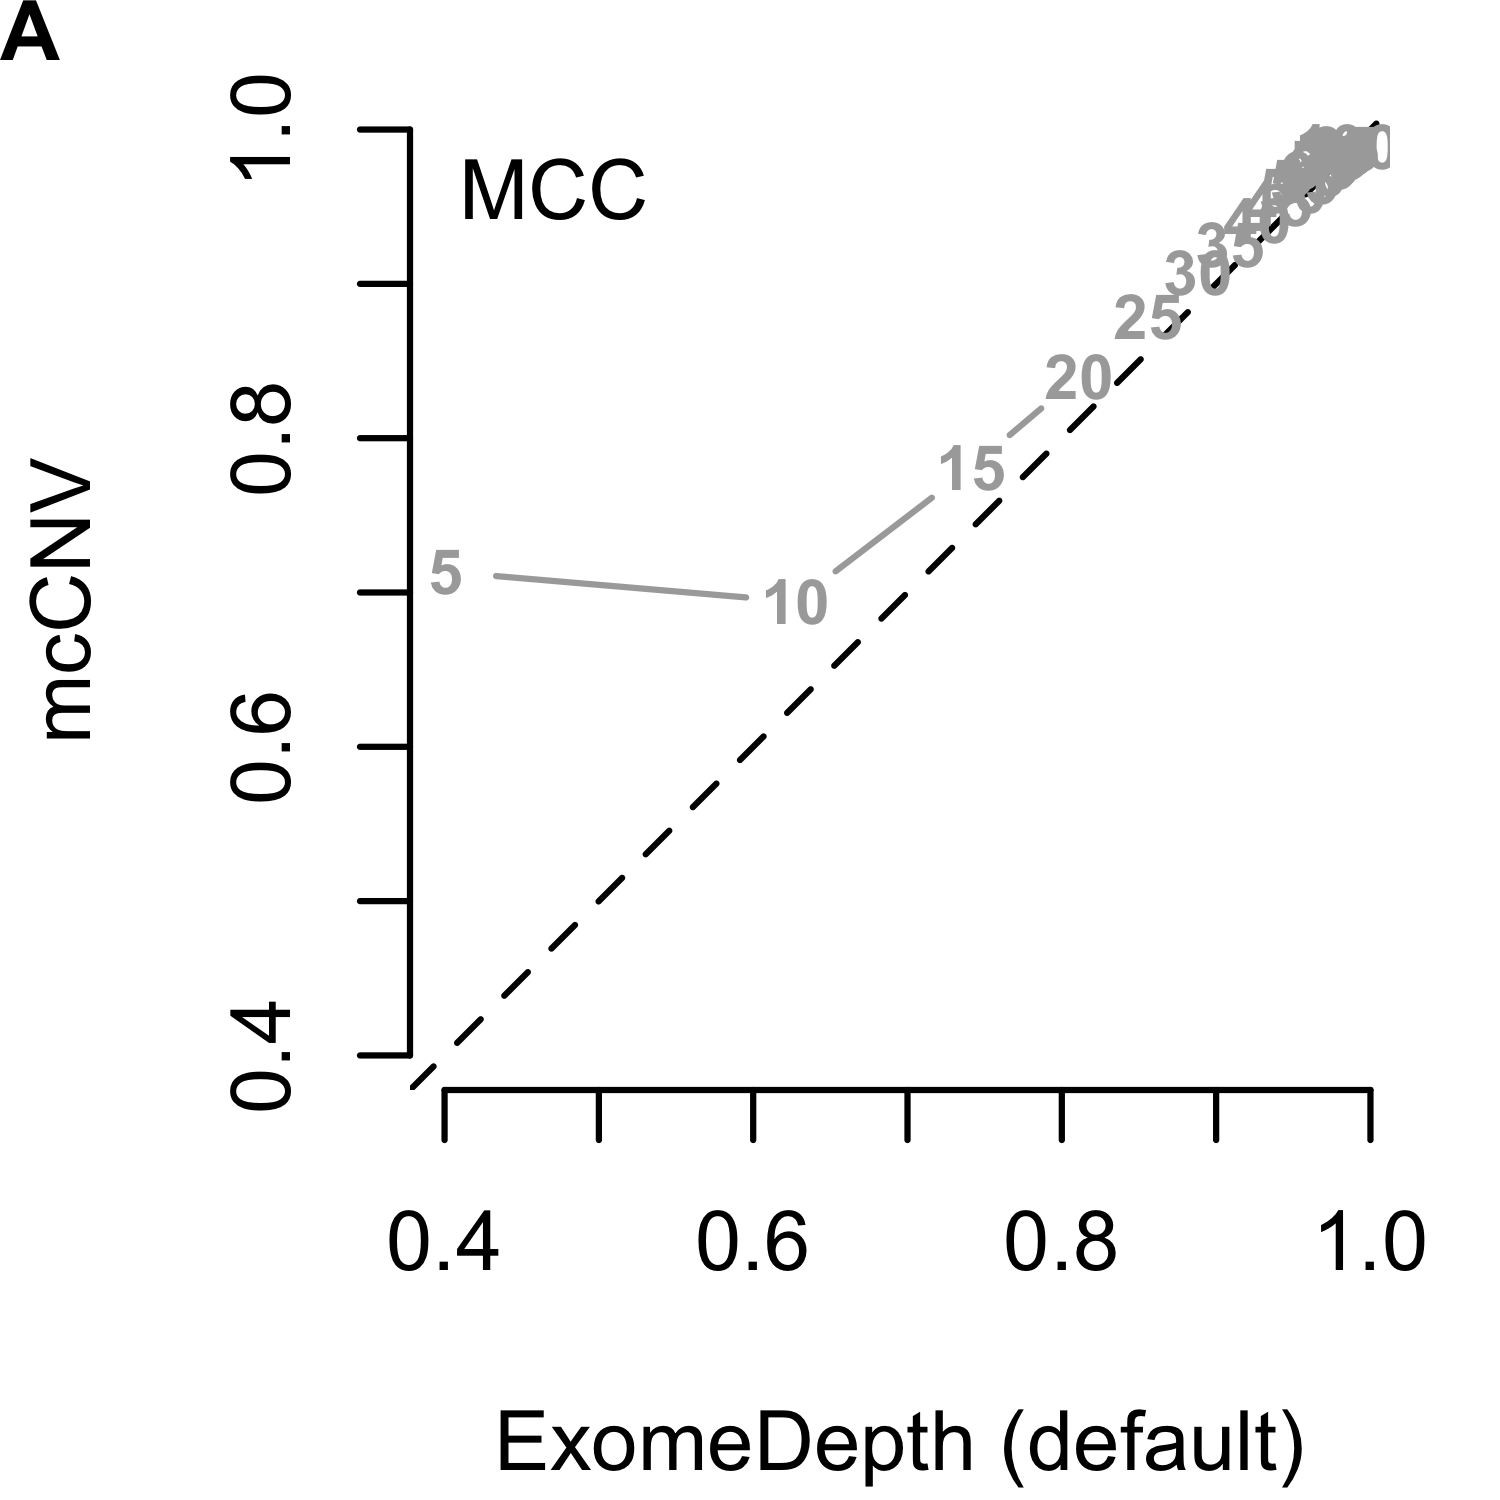
\includegraphics[width=0.32\linewidth]{DLFilerDissertation_files/figure-latex/simRes-1} 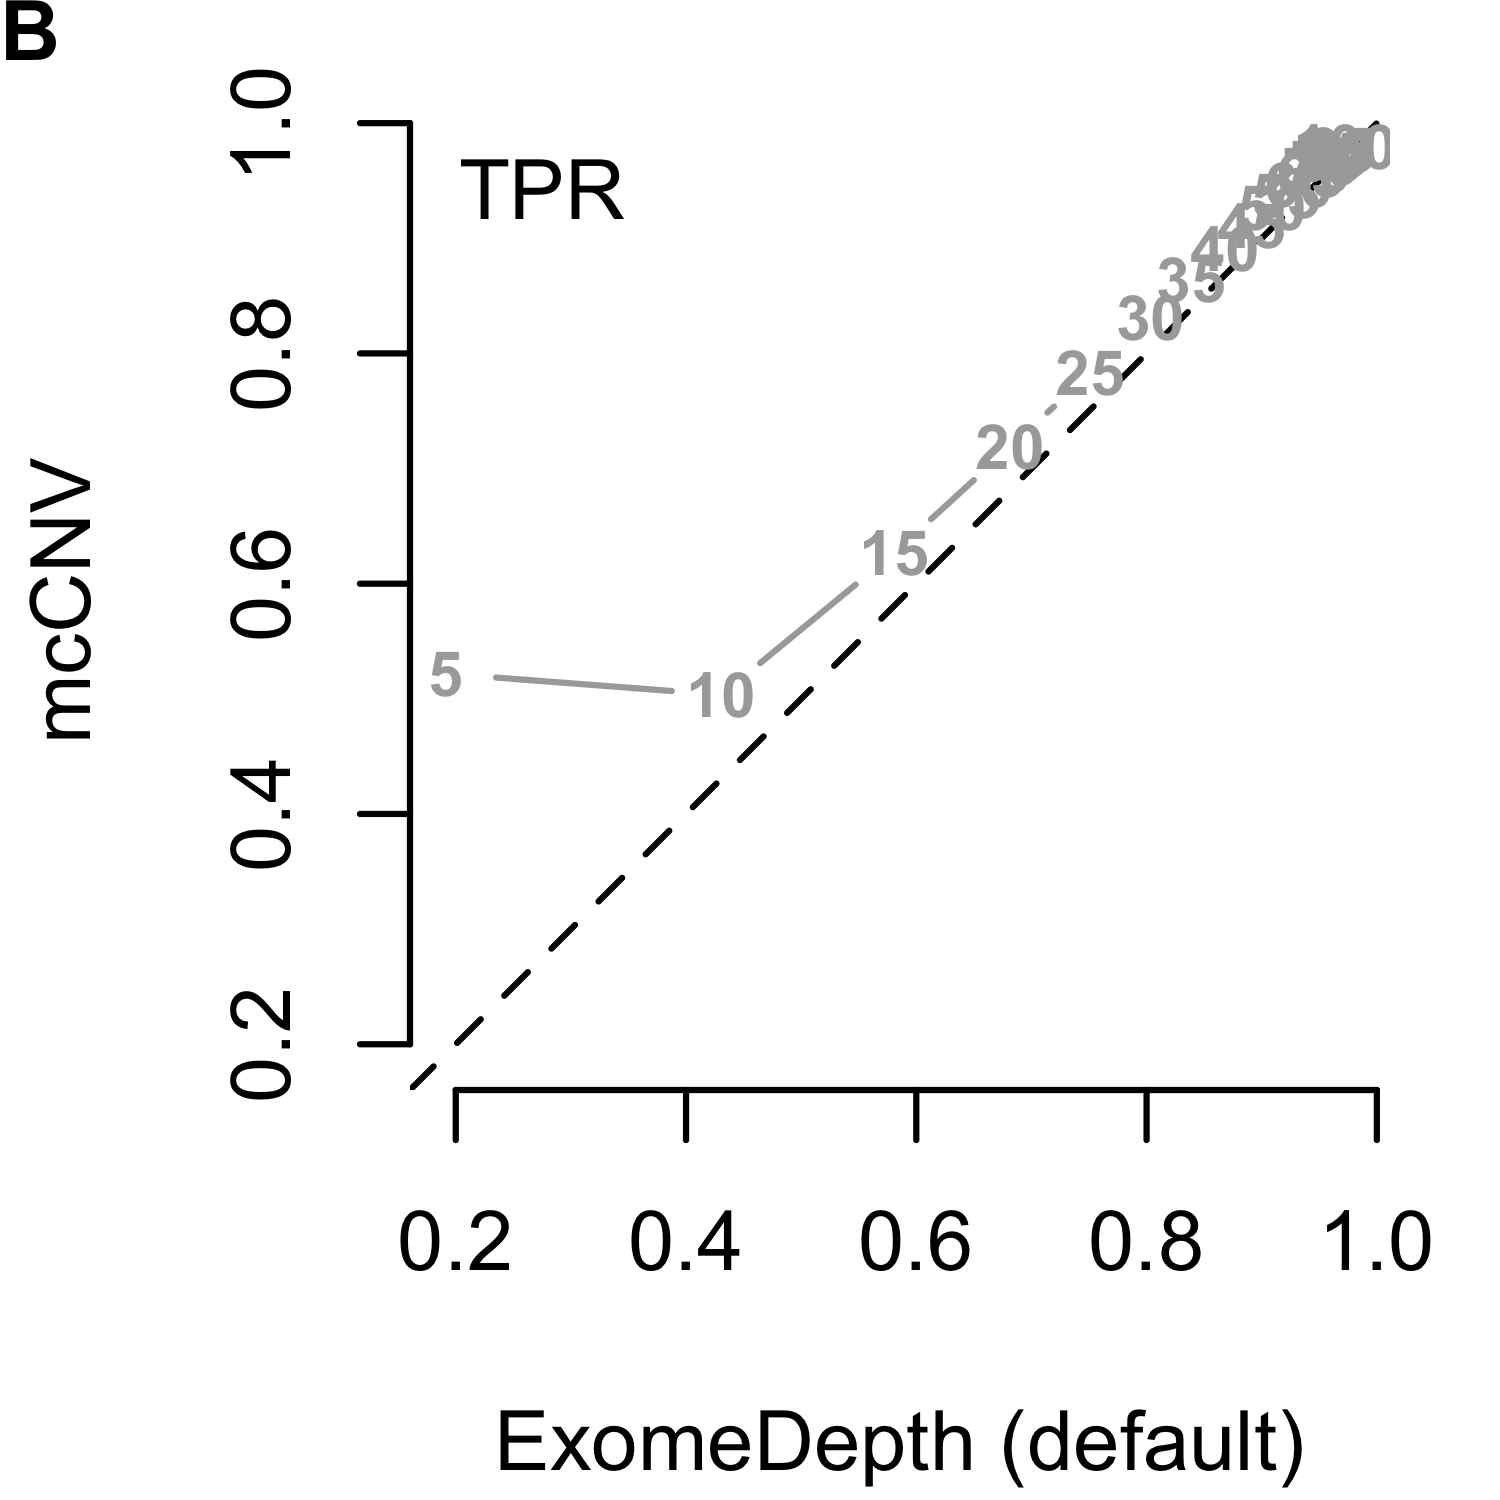
\includegraphics[width=0.32\linewidth]{DLFilerDissertation_files/figure-latex/simRes-2} 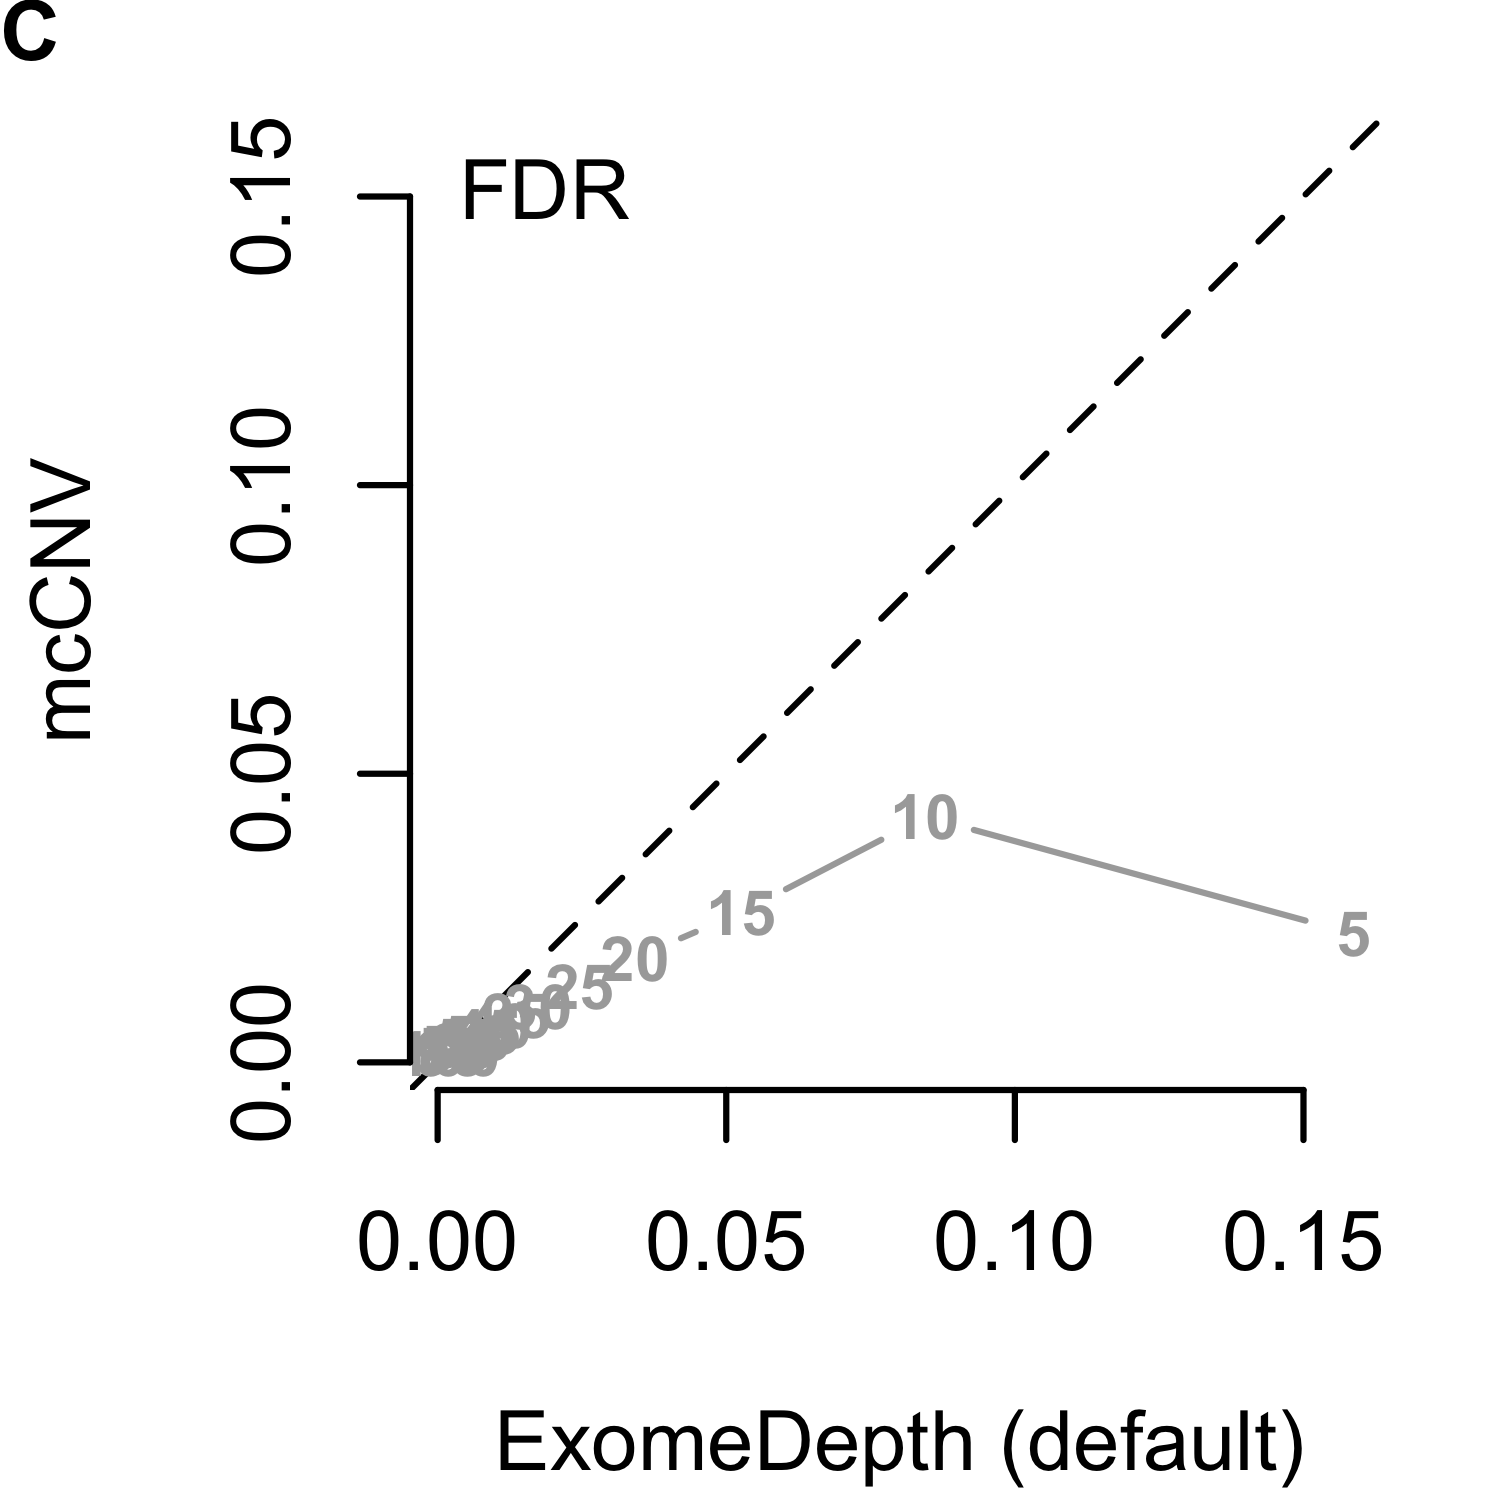
\includegraphics[width=0.32\linewidth]{DLFilerDissertation_files/figure-latex/simRes-3} 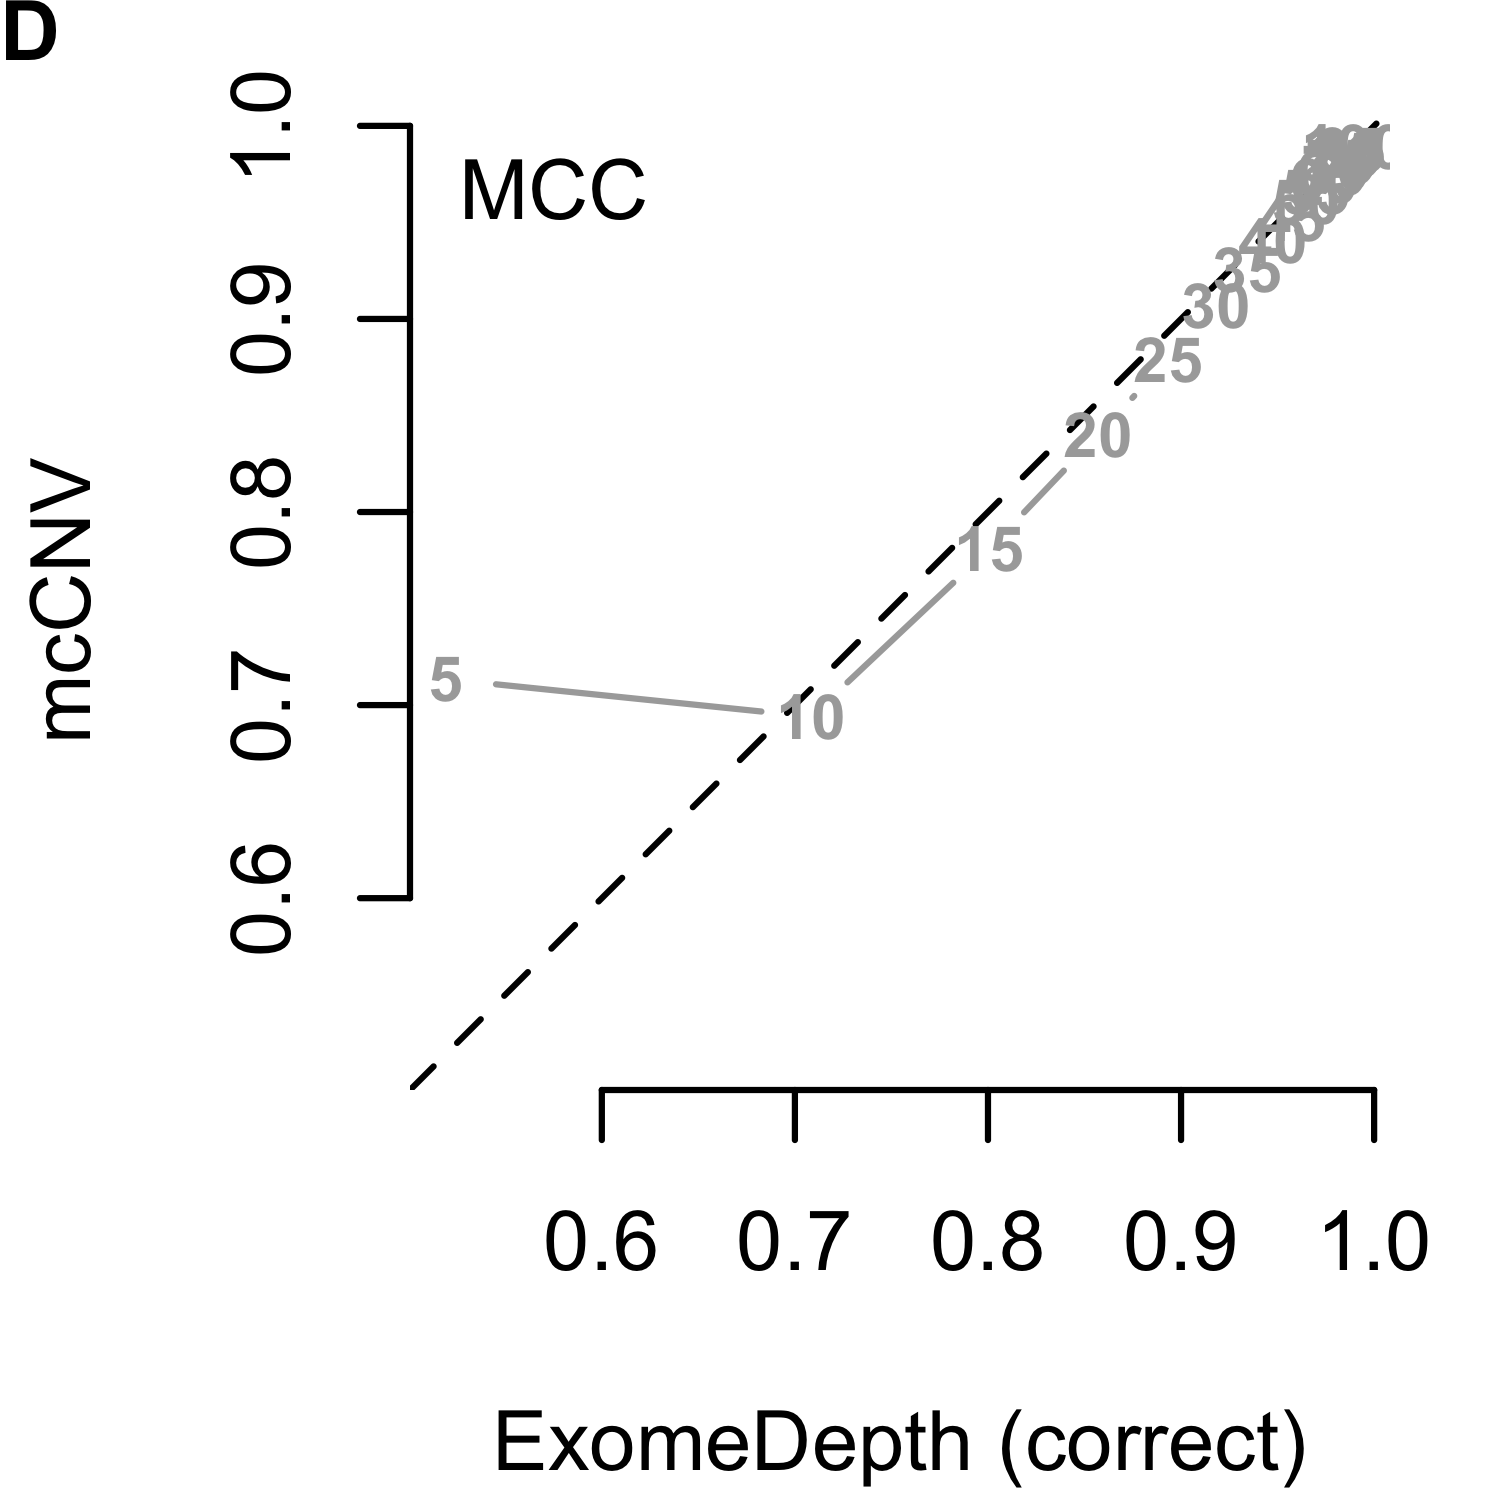
\includegraphics[width=0.32\linewidth]{DLFilerDissertation_files/figure-latex/simRes-4} 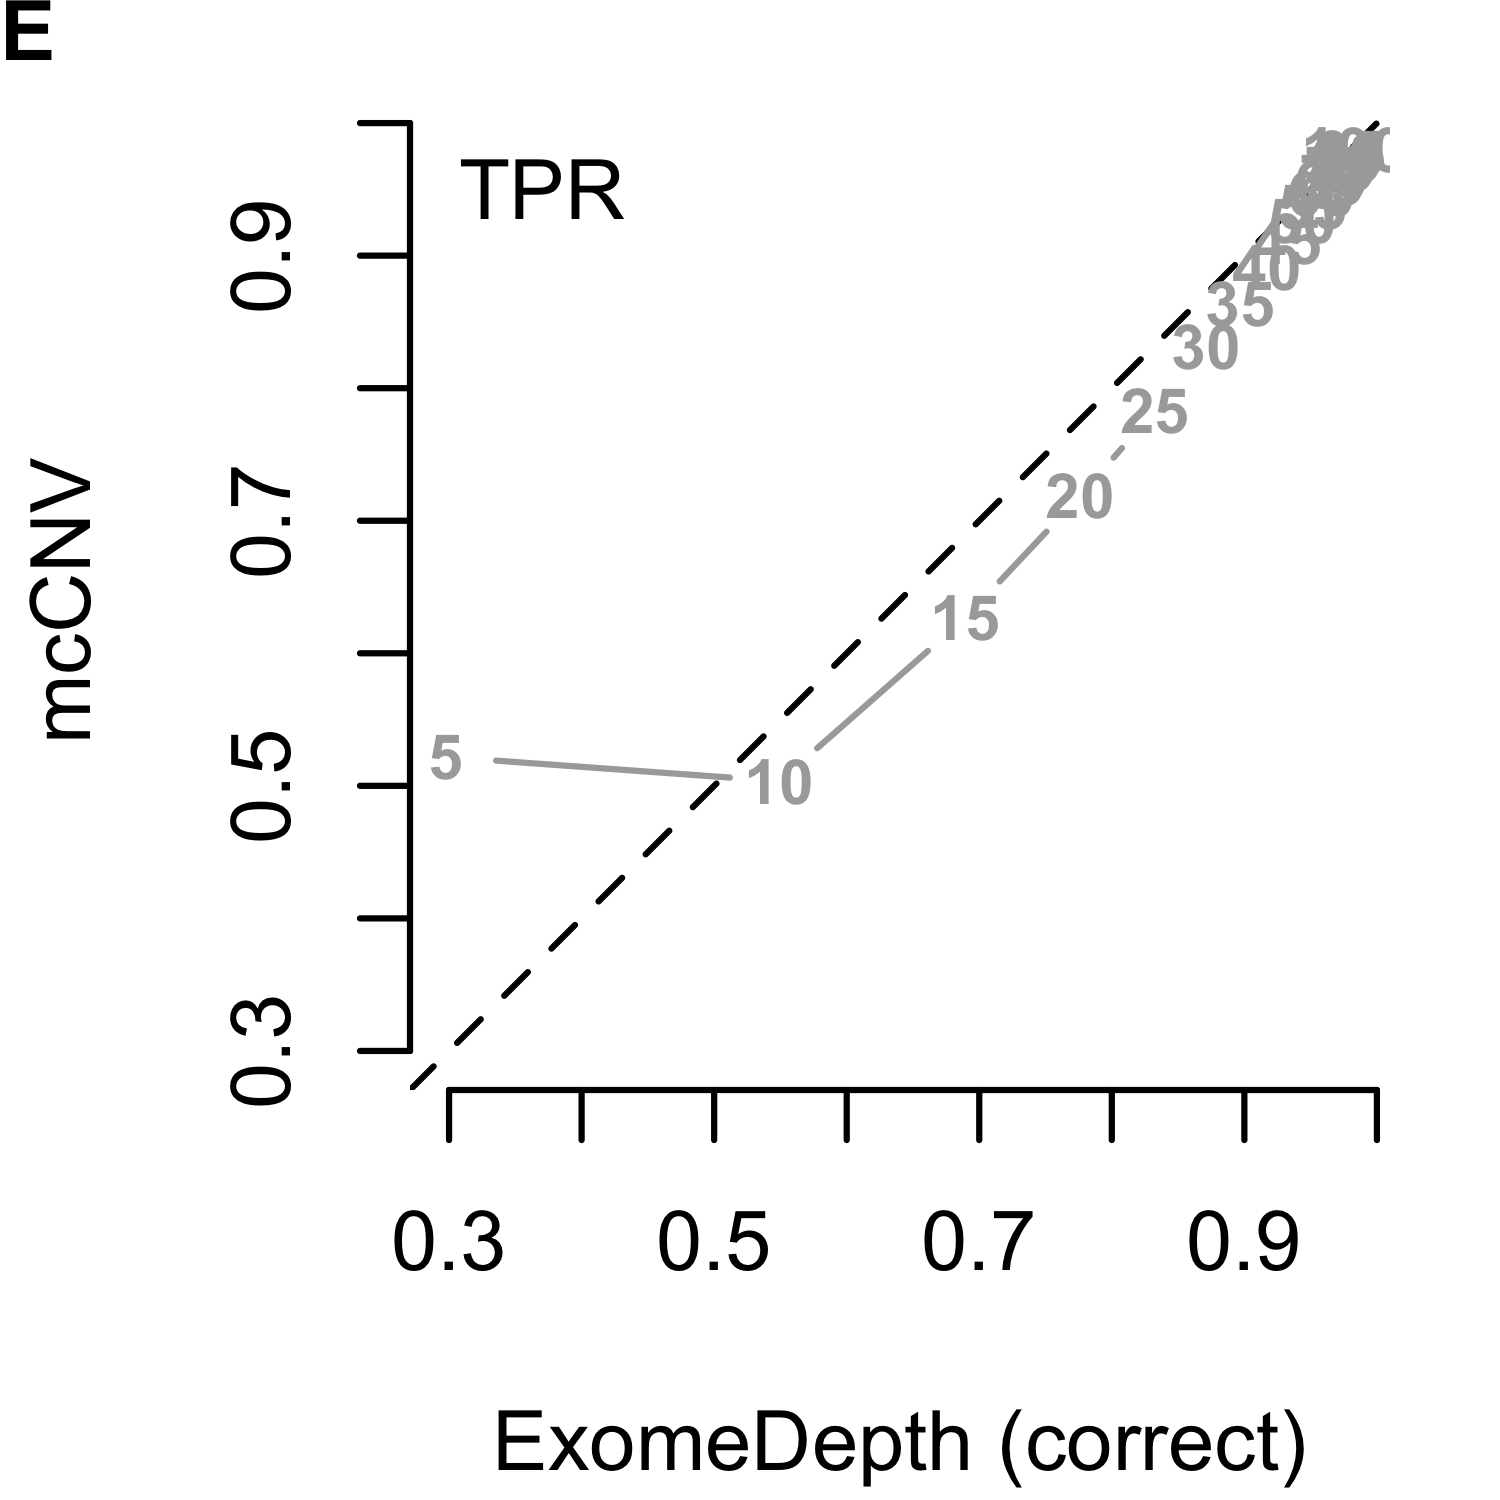
\includegraphics[width=0.32\linewidth]{DLFilerDissertation_files/figure-latex/simRes-5} 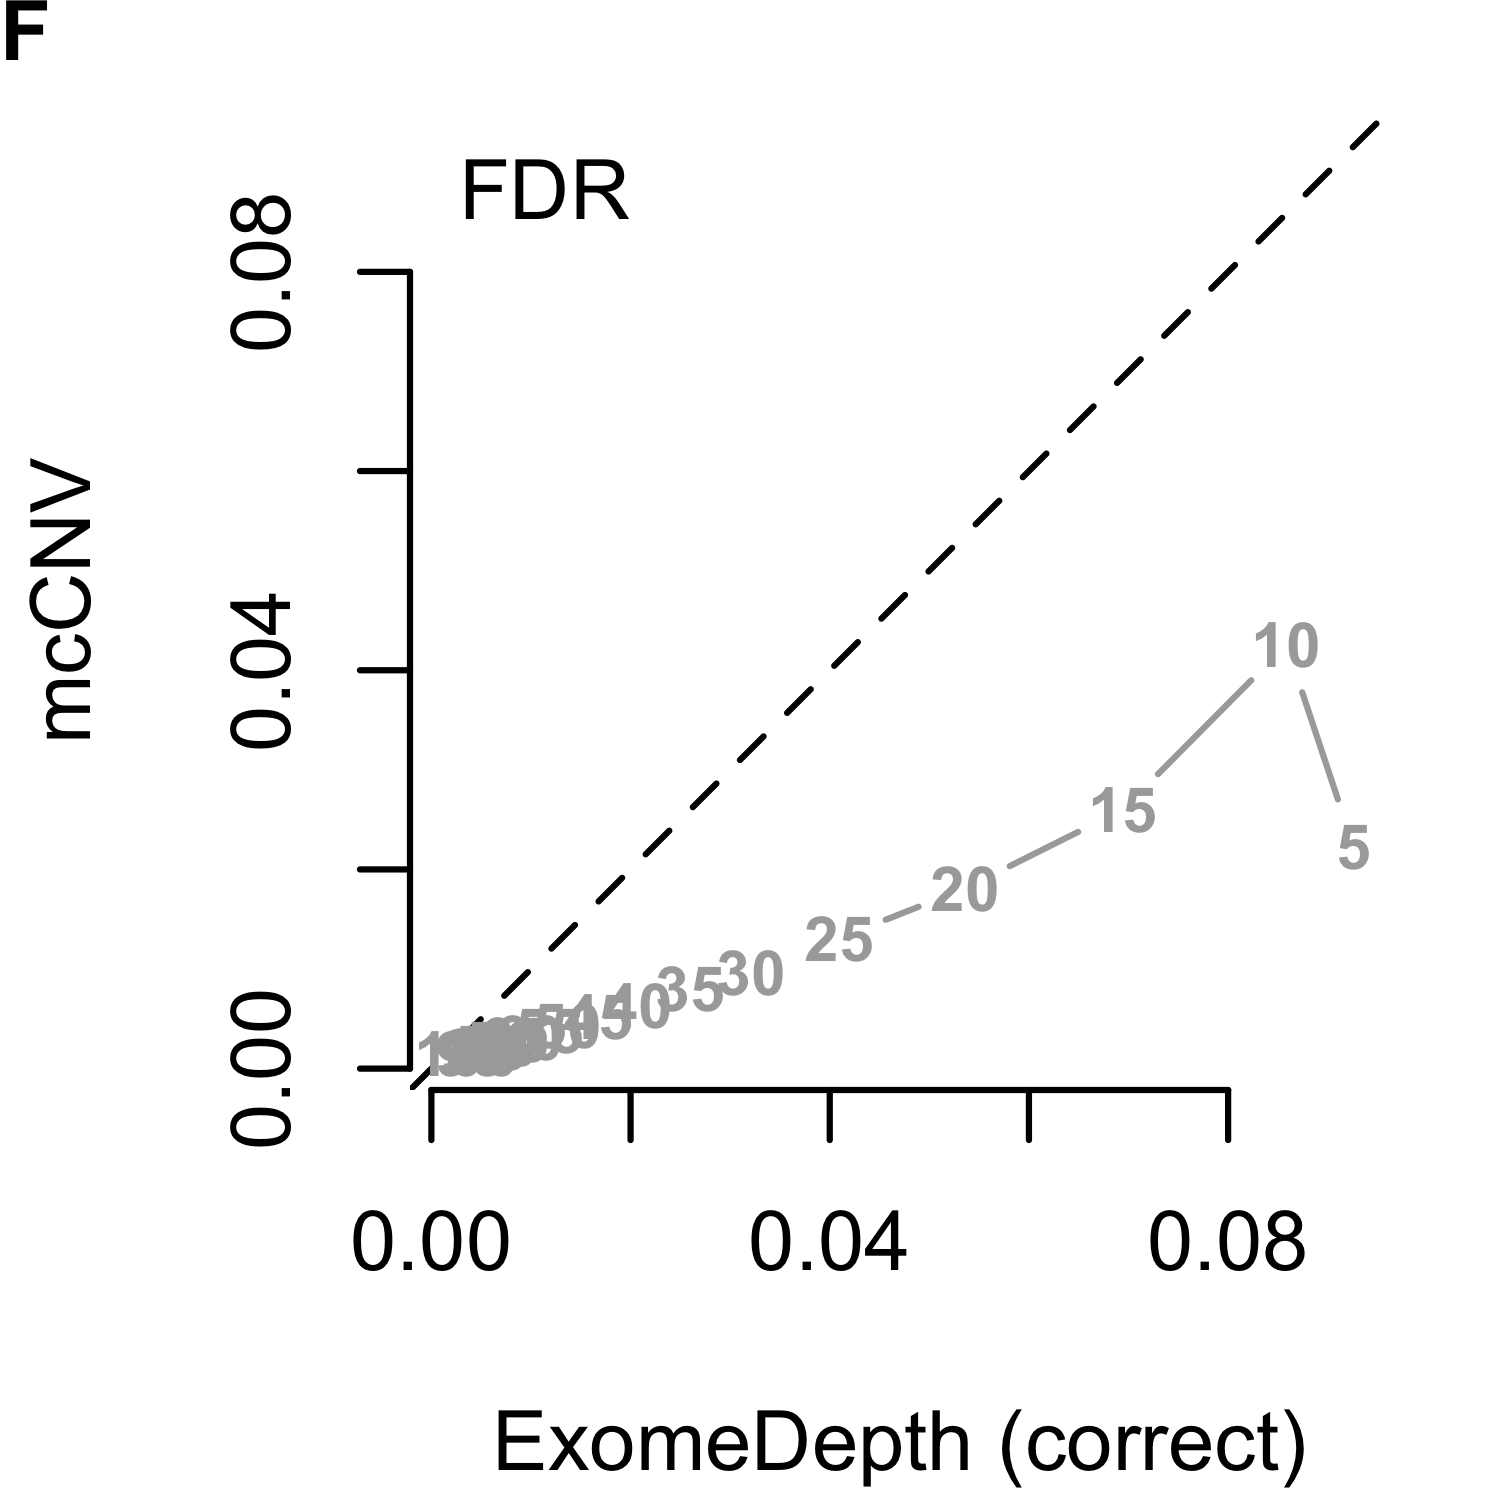
\includegraphics[width=0.32\linewidth]{DLFilerDissertation_files/figure-latex/simRes-6} 

}

\caption[Algorithm performance comparing mcCNV and ExomeDepth on simulated exomes.]{Algorithm performance comparing mcCNV and ExomeDepth on simulated exomes. (A-C) mcCNV versus ExomeDepth with default parameters, \(1/10,000\) transition probability and 50 kb expected variant length. (D-F) mcCNV versus ExomeDepth with simulation-matched parameters, \(1/1,000\) transition probability and 1 kb expected variant length. Numbered points indicate the simulated depth in millions of molecules. `MCC' indicates Matthew's correlation coefficient; `TPR' indicates true positive rate/sensitivity; `FDR' indicates false discovery rate. Dashed black line shows the 1:1 relationship.}\label{fig:simRes}
\end{figure}



\begin{table}

\caption[Algorithm performance comparing mcCNV and ExomeDepth on simulated exomes.]{\label{tab:simResTbl}Simulation results by algorithm. ED-def: ExomeDepth with default parameters; ED-sim: ExomeDepth with simulation-matched parameters. Values represent the mean over 200 simulations.}
\centering
\begin{tabular}[t]{rrrrrrrrrr}
\toprule
\multicolumn{1}{c}{ } & \multicolumn{3}{c}{MCC} & \multicolumn{3}{c}{TPR} & \multicolumn{3}{c}{FDR} \\
\cmidrule(l{3pt}r{3pt}){2-4} \cmidrule(l{3pt}r{3pt}){5-7} \cmidrule(l{3pt}r{3pt}){8-10}
dep & mcCNV & ED-def & ED-sim & mcCNV & ED-def & ED-sim & mcCNV & ED-def & ED-sim\\
\midrule
5 & 0.713 & 0.401 & 0.519 & 0.522 & 0.192 & 0.298 & 0.02230 & 0.15900 & 0.09260\\
10 & 0.694 & 0.628 & 0.708 & 0.503 & 0.431 & 0.549 & 0.04250 & 0.08450 & 0.08590\\
15 & 0.781 & 0.742 & 0.801 & 0.627 & 0.581 & 0.690 & 0.02600 & 0.05270 & 0.06940\\
20 & 0.840 & 0.811 & 0.857 & 0.719 & 0.682 & 0.777 & 0.01810 & 0.03420 & 0.05360\\
25 & 0.879 & 0.856 & 0.893 & 0.783 & 0.752 & 0.832 & 0.01310 & 0.02460 & 0.04090\\
\addlinespace
30 & 0.907 & 0.889 & 0.918 & 0.831 & 0.804 & 0.872 & 0.00967 & 0.01750 & 0.03210\\
35 & 0.926 & 0.909 & 0.935 & 0.864 & 0.839 & 0.897 & 0.00807 & 0.01370 & 0.02600\\
40 & 0.941 & 0.927 & 0.948 & 0.891 & 0.869 & 0.917 & 0.00638 & 0.01060 & 0.02080\\
45 & 0.952 & 0.940 & 0.957 & 0.911 & 0.892 & 0.932 & 0.00527 & 0.00846 & 0.01680\\
50 & 0.961 & 0.950 & 0.965 & 0.927 & 0.910 & 0.944 & 0.00437 & 0.00701 & 0.01370\\
\addlinespace
55 & 0.966 & 0.957 & 0.969 & 0.937 & 0.921 & 0.951 & 0.00377 & 0.00569 & 0.01180\\
60 & 0.972 & 0.963 & 0.974 & 0.947 & 0.933 & 0.959 & 0.00318 & 0.00517 & 0.00986\\
65 & 0.976 & 0.969 & 0.978 & 0.955 & 0.943 & 0.964 & 0.00290 & 0.00433 & 0.00837\\
70 & 0.978 & 0.972 & 0.980 & 0.960 & 0.949 & 0.968 & 0.00252 & 0.00381 & 0.00735\\
75 & 0.981 & 0.976 & 0.983 & 0.965 & 0.955 & 0.972 & 0.00212 & 0.00321 & 0.00625\\
\addlinespace
80 & 0.983 & 0.978 & 0.985 & 0.969 & 0.960 & 0.975 & 0.00200 & 0.00294 & 0.00560\\
85 & 0.985 & 0.980 & 0.986 & 0.972 & 0.963 & 0.977 & 0.00181 & 0.00263 & 0.00491\\
90 & 0.987 & 0.982 & 0.987 & 0.975 & 0.967 & 0.979 & 0.00169 & 0.00243 & 0.00451\\
95 & 0.988 & 0.984 & 0.988 & 0.978 & 0.970 & 0.981 & 0.00156 & 0.00223 & 0.00393\\
100 & 0.989 & 0.985 & 0.989 & 0.980 & 0.973 & 0.982 & 0.00150 & 0.00195 & 0.00359\\
\bottomrule
\end{tabular}
\end{table}

\hypertarget{mccnv-exomedepth-perform-comparably-on-wgs-pool}{%
\subsection{mcCNV \& ExomeDepth perform comparably on WGS pool}\label{mccnv-exomedepth-perform-comparably-on-wgs-pool}}

To establish a truth set on real data, we performed matched genome sequencing on the subjects included in the WGS pool.
Following the best practices suggested by Trost et al.~\textsuperscript{\protect\hyperlink{ref-trost:2018aa}{98}}, we performed read-depth based CNV calling using the genome data.
In line with recommendations by Trost et al., we excluded from comparative analysis any exons overlapping repetitive or low-complexity regions (34,856 out of 179,250).
We then compared the exome calls using mcCNV and ExomeDepth to the genome calls using the overlap of ERDS and cnvpytor.
Table \ref{tab:wgsCallSbj} lists the total calls by subject.
Overall, mcCNV predicted the largest number of variants; however, 85.7\% of predicted variants were deletions from two samples (NCG\_00790 and NCG\_00851).
ExomeDepth also predicted a disproportionate number of deletions for NCG\_00790 and NCG\_00851, totaling 69.4\% of calls.



\begin{table}

\caption[Number of CNV calls by subject and algorithm for the 'WGS' pool.]{\label{tab:wgsCallSbj}Number of CNV calls by subject and algorithm for the `WGS' pool. `MC' indicates the mcCNV algorithm; `ED' indicates the ExomeDepth algorithm; `WG' indicates the overlap of ERDS/cnvpytor calls from matched whole-genome sequencing. Exons with any overlap of the repetitive and low-complexity regions, as defined in the Trost et al.~manuscript,\textsuperscript{\protect\hyperlink{ref-trost:2018aa}{98}} omitted from analysis.}
\centering
\begin{tabular}[t]{lrrrrrrrrr}
\toprule
\multicolumn{1}{c}{ } & \multicolumn{3}{c}{Total} & \multicolumn{3}{c}{Duplications} & \multicolumn{3}{c}{Deletions} \\
\cmidrule(l{3pt}r{3pt}){2-4} \cmidrule(l{3pt}r{3pt}){5-7} \cmidrule(l{3pt}r{3pt}){8-10}
subject & MC & ED & WG & MC & ED & WG & MC & ED & WG\\
\midrule
NCG\_00012 & 90 & 106 & 143 & 61 & 73 & 121 & 29 & 33 & 22\\
NCG\_00237 & 82 & 101 & 165 & 50 & 64 & 129 & 32 & 37 & 36\\
NCG\_00525 & 68 & 74 & 151 & 30 & 33 & 110 & 38 & 41 & 41\\
NCG\_00593 & 45 & 58 & 142 & 22 & 28 & 81 & 23 & 30 & 61\\
NCG\_00676 & 66 & 78 & 112 & 38 & 46 & 92 & 28 & 32 & 20\\
\addlinespace
NCG\_00790 & 5,156 & 2,204 & 121 & 19 & 37 & 92 & 5,137 & 2,167 & 29\\
NCG\_00819 & 68 & 76 & 134 & 30 & 41 & 100 & 38 & 35 & 34\\
NCG\_00840 & 78 & 92 & 157 & 44 & 52 & 115 & 34 & 40 & 42\\
NCG\_00851 & 1,151 & 859 & 141 & 28 & 51 & 102 & 1,123 & 808 & 39\\
NCG\_00857 & 59 & 75 & 119 & 10 & 15 & 81 & 49 & 60 & 38\\
\addlinespace
NCG\_00976 & 46 & 58 & 114 & 25 & 37 & 93 & 21 & 21 & 21\\
NCG\_01023 & 59 & 95 & 143 & 32 & 60 & 113 & 27 & 35 & 30\\
NCG\_01043 & 73 & 94 & 128 & 40 & 64 & 105 & 33 & 30 & 23\\
NCG\_01076 & 36 & 57 & 105 & 7 & 22 & 78 & 29 & 35 & 27\\
NCG\_01077 & 135 & 157 & 230 & 103 & 121 & 184 & 32 & 36 & 46\\
\addlinespace
NCG\_01117 & 95 & 101 & 154 & 72 & 78 & 129 & 23 & 23 & 25\\
\bottomrule
\end{tabular}
\end{table}

Looking at the control selection, for NCG\_00790 and NCG\_00851 ExomeDepth only selected 2 and 3 controls, respectively.
Furthermore, NCG\_00790 and NCG\_00851 had substantially higher dispersion than the rest of the pool (two outliers in Figure \ref{fig:edSelPhi}).

Recognizing the genome calls do not represent an accurate truth set, we looked at the ability of mcCNV and ExomeDepth to predict the genome calls.
Due to the large number of deletions called for NCG\_00790 and NCG\_00851, both algorithms performed poorly in predicting the genome calls (Table \ref{tab:predMet}).
When we excluded NCG\_00790 and NCG\_00851 from the analysis, mcCNV had comparable, but uniformly better performance.
Both algorithms demonstrated greater power to detect deletions.
Figures \ref{fig:wgsVennAll} and \ref{fig:wgsVennSub} show the call overlap between the three approaches, including and excluding NCG\_00790 and NCG\_00851, respectively.



\begin{table}

\caption[mcCNV and ExomeDepth performance predicting calls from genome sequencing.]{\label{tab:predMet}mcCNV (MC)/ExomeDepth (ED) calls for `WGS' pool (used as prediction) versus the ERDS/cnvpytor calls from matched genome sequencing (used as truth). Calls are subdivided by duplications (DUP) and deletions (DEL). `Full' gives performance across the full pool; `Sub' gives the performance excluding the poorly correlated samples NCG\_00790 and NCG\_00851 (gray rows). `MCC' is Matthew's correlation coefficient, `TPR' is true positive rate/sensitivity, `FDR' is false discovery rate, `PPV' is positive predictive value, `BalAcc' is balanced accuracy. Exons with any overlap of the repetitive and low-complexity regions, as defined in the Trost et al.~manuscript,\textsuperscript{\protect\hyperlink{ref-trost:2018aa}{98}} omitted from analysis.}
\centering
\begin{tabular}[t]{lllrrrr}
\toprule
 &  &  & MCC & TPR & FDR & PPV\\
\midrule
 &  & MC & 0.185 & 0.335 & 0.897 & 0.1030\\
\cmidrule{3-7}
 & \multirow{-2}{*}{\raggedright\arraybackslash Total} & ED & 0.263 & 0.363 & 0.809 & 0.1910\\
\cmidrule{2-7}
 &  & MC & 0.487 & 0.345 & 0.311 & 0.6890\\
\cmidrule{3-7}
\multirow{-4}{*}{\raggedright\arraybackslash ALL} & \multirow{-2}{*}{\raggedright\arraybackslash Sub} & ED & 0.482 & 0.378 & 0.383 & 0.6170\\
\cmidrule{1-7}
 &  & MC & 0.396 & 0.236 & 0.334 & 0.6660\\
\cmidrule{3-7}
 & \multirow{-2}{*}{\raggedright\arraybackslash Total} & ED & 0.347 & 0.240 & 0.496 & 0.5040\\
\cmidrule{2-7}
 &  & MC & 0.404 & 0.246 & 0.333 & 0.6670\\
\cmidrule{3-7}
\multirow{-4}{*}{\raggedright\arraybackslash DUP} & \multirow{-2}{*}{\raggedright\arraybackslash Sub} & ED & 0.384 & 0.266 & 0.446 & 0.5540\\
\cmidrule{1-7}
 &  & MC & 0.180 & 0.639 & 0.949 & 0.0509\\
\cmidrule{3-7}
 & \multirow{-2}{*}{\raggedright\arraybackslash Total} & ED & 0.219 & 0.558 & 0.914 & 0.0861\\
\cmidrule{2-7}
 &  & MC & 0.683 & 0.661 & 0.294 & 0.7060\\
\cmidrule{3-7}
\multirow{-4}{*}{\raggedright\arraybackslash DEL} & \multirow{-2}{*}{\raggedright\arraybackslash Sub} & ED & 0.541 & 0.554 & 0.471 & 0.5290\\
\bottomrule
\end{tabular}
\end{table}





\begin{figure}

{\centering 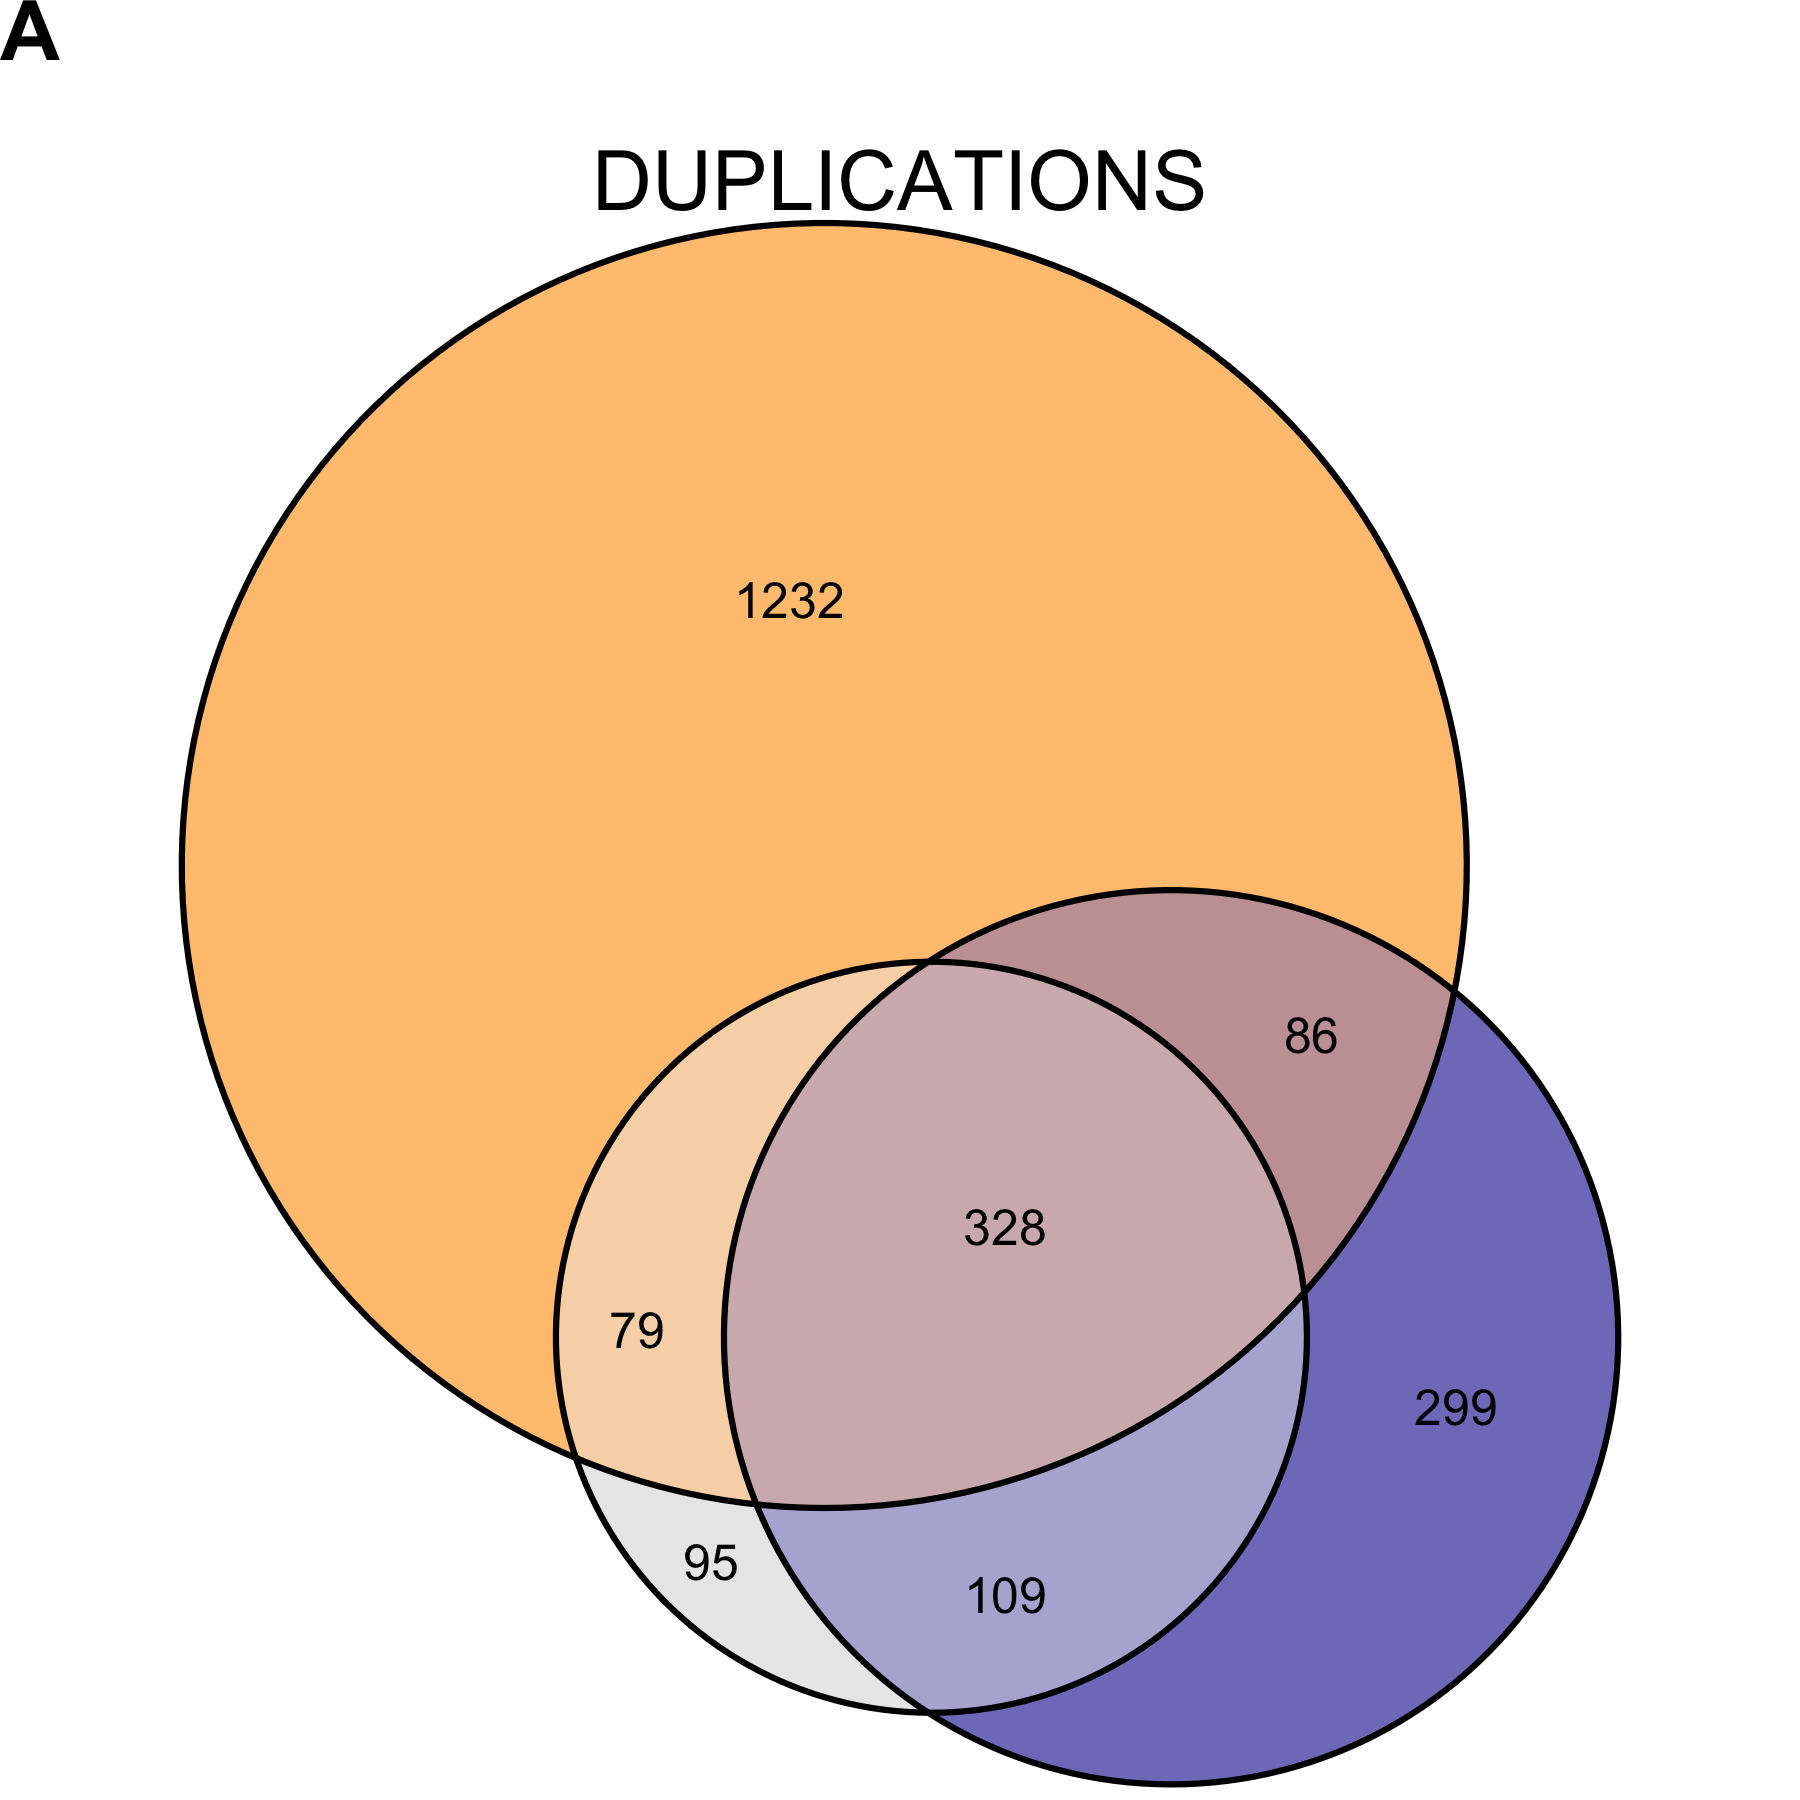
\includegraphics[width=0.49\linewidth]{DLFilerDissertation_files/figure-latex/wgsVennAll-1} 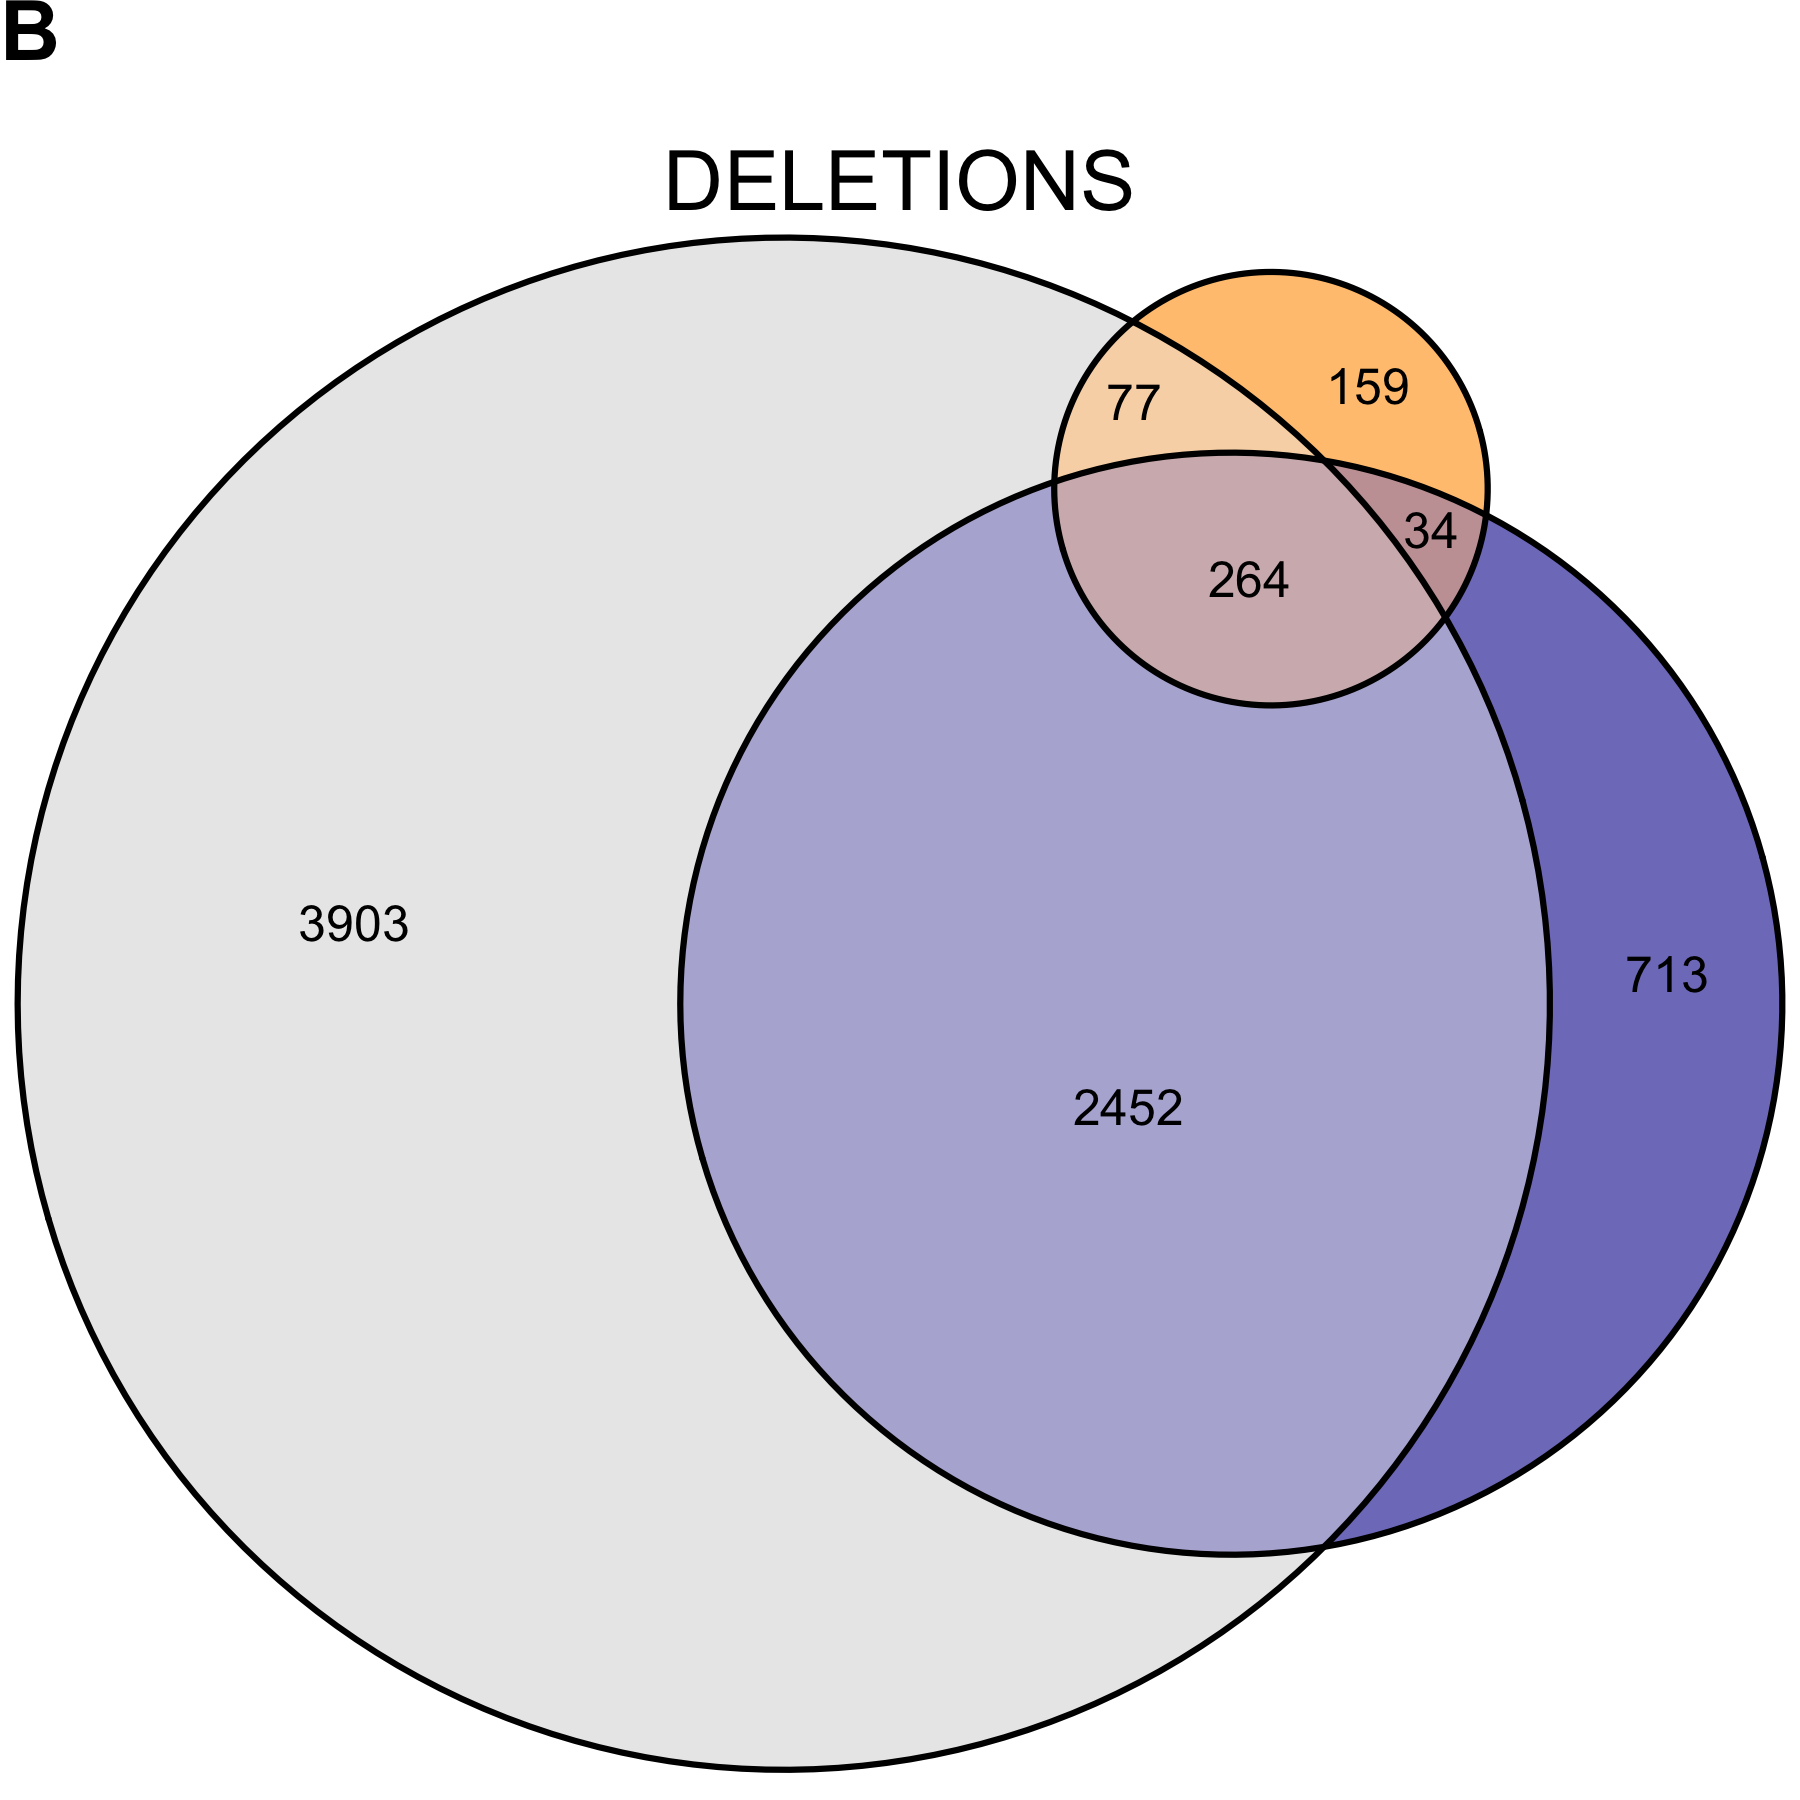
\includegraphics[width=0.49\linewidth]{DLFilerDissertation_files/figure-latex/wgsVennAll-2} 

}

\caption[Copy number variant call concordance for the WGS pool.]{Copy number variant call concordance for the WGS pool. (A) predicted duplications; (B) predicted deletions. mcCNV in grey; ExomeDepth in blue; ERDS/cnvpytor in orange. Values within overlaps give the number of variants.}\label{fig:wgsVennAll}
\end{figure}



\begin{figure}

{\centering 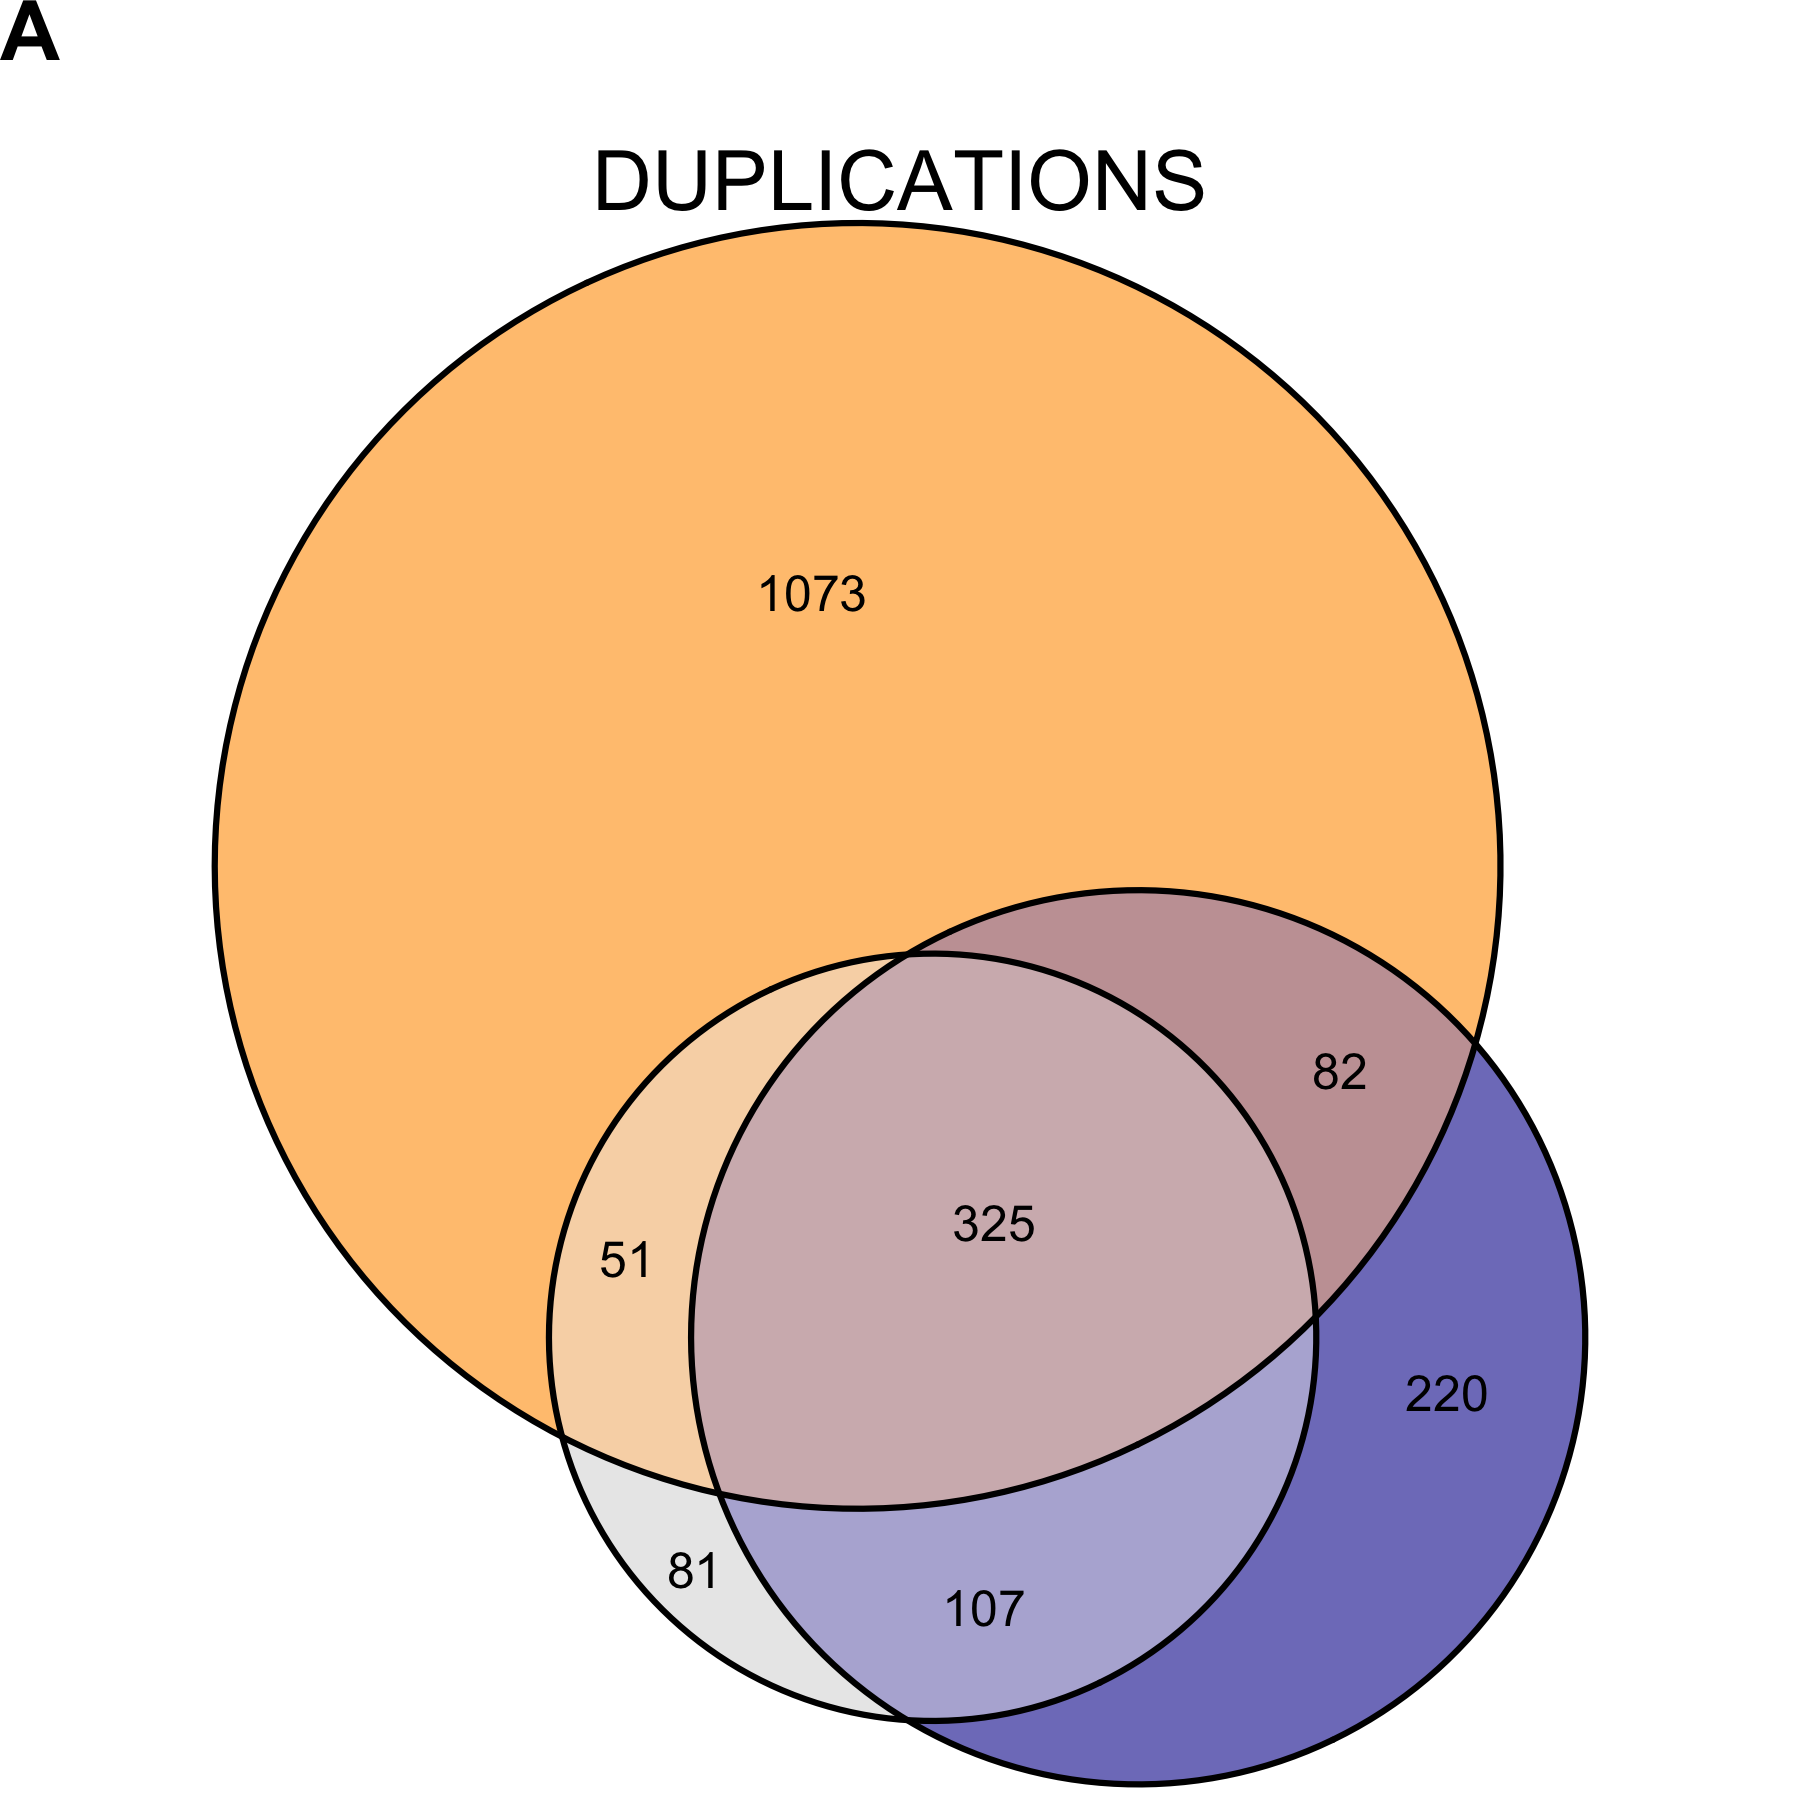
\includegraphics[width=0.49\linewidth]{DLFilerDissertation_files/figure-latex/wgsVennSub-1} 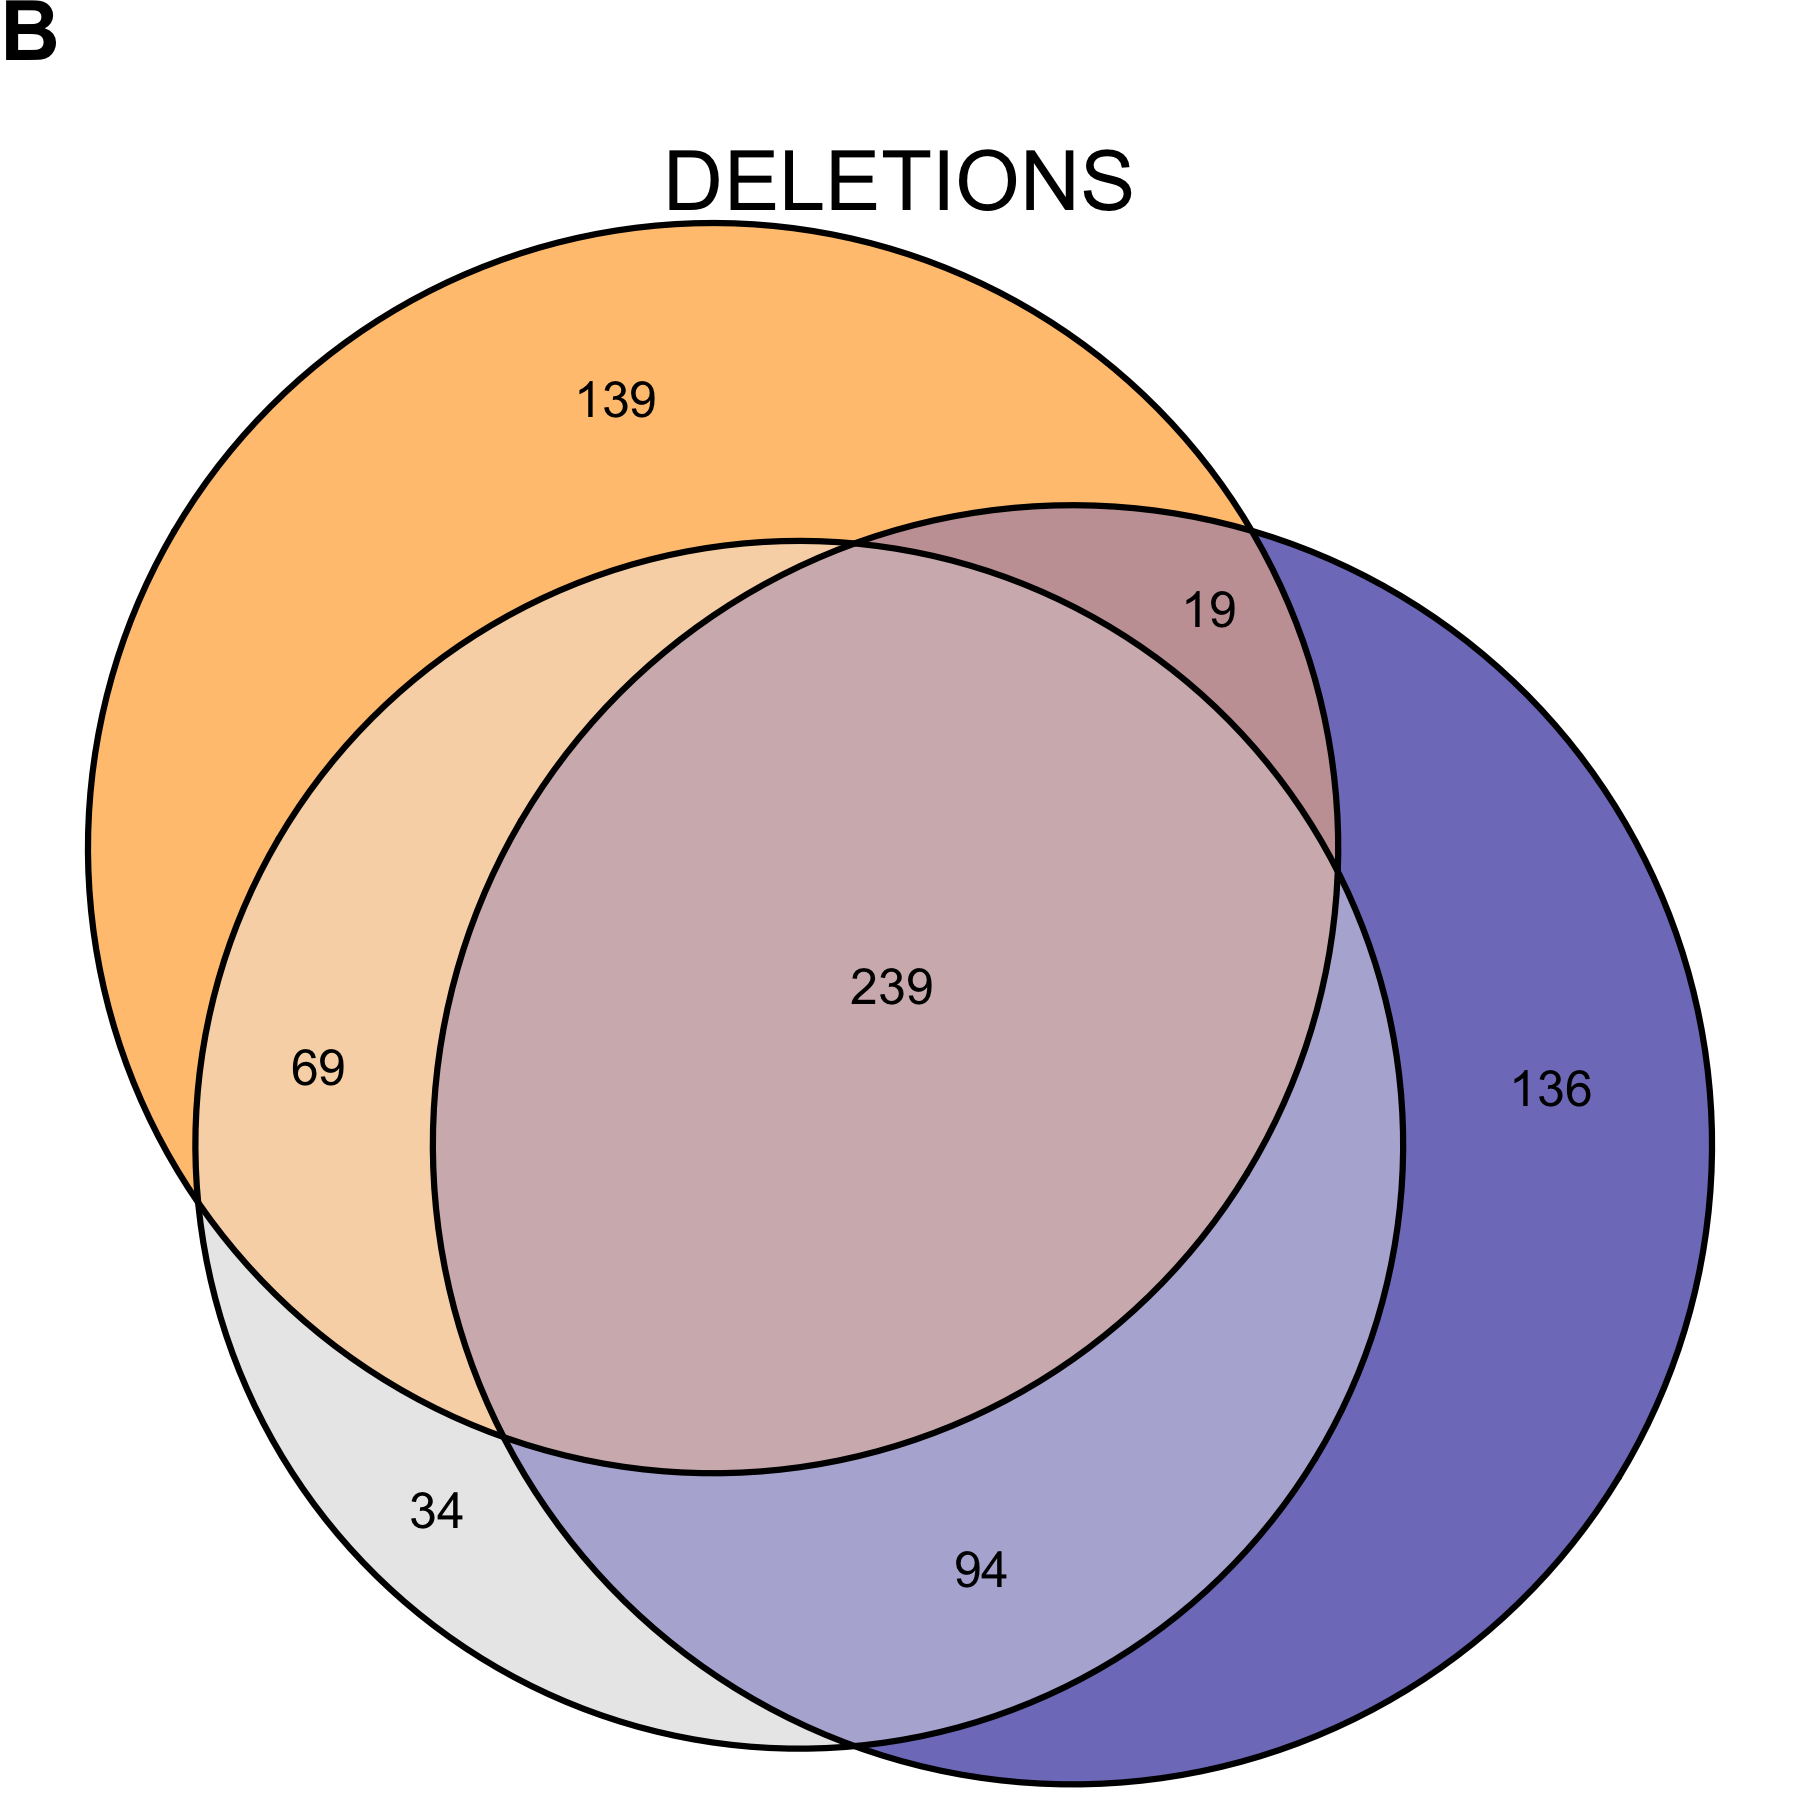
\includegraphics[width=0.49\linewidth]{DLFilerDissertation_files/figure-latex/wgsVennSub-2} 

}

\caption[Copy number variant call concordance for the WGS pool, excluding subjects NCG\_00790 and NCG\_00851 due to poor correlation to the rest of the pool.]{Copy number variant call concordance for the WGS pool, excluding subjects NCG\_00790 and NCG\_00851 due to poor correlation to the rest of the pool. (A) predicted duplications; (B) predicted deletions. mcCNV in grey; ExomeDepth in blue; ERDS/cnvpytor in orange. Values within overlaps give the number of variants.}\label{fig:wgsVennSub}
\end{figure}

\hypertarget{discussion}{%
\section{Discussion}\label{discussion}}

The medical genetics community still lacks robust exome-wide information about small (exon-level) variant prevalence.
Others have established the reliability and cost-efficiency of pre-capture multiplexing,\textsuperscript{\protect\hyperlink{ref-neiman:2012aa}{103}--\protect\hyperlink{ref-shearer:2012aa}{107}} and most commercial exome capture platforms have protocols for pre-capture multiplexing.
Here, we demonstrate the reduction in inter-sample variance when pre-capture multiplexing, leading to increased power to detect exon-level copy number variation.
Despite the benefits, many clinical laboratories do not employ a multiplexed capture protocol because multiplexing requires waiting to fill a pool and may delay results.
While we understand the increased complexity, multiplexed capture may uncover otherwise missed copy number variation and increase the diagnostic yield for patients.

Multiplexed capture is not without limitations.
We presented an example (pool IDT-MC) where multiplexed capture provided little to no improvement over independently-captured samples.
We concluded the absent improvement in inter-sample variance stemmed from the poor library balance prior to capture.
Rebuilding a more-balanced pool with the same samples (pool IDT-RR) demonstrated a large reduction in inter-sample variance.

In assessing the inter-sample variance, we compared two capture platforms: (1) Agilent SureSelectXT2 and (2) Integrated DNA Technologies xGen Lockdown Probes.
We do not have enough data to suggest definitively one over the other.
Comparing the mean-variance relationship, the IDT-RR pool appeared to have less dispersion overall (Figure \ref{fig:mnVrComp}); however, the sample-specific dispersion estimates from ExomeDepth suggest better performance by the WGS pool (Figure \ref{fig:edSelPhi}) and the higher pool-wide dispersion comes entirely from the two poorly correlated samples.

Our results suggest having a sufficiently large database of samples most-often provides appropriate control samples to estimate copy number variation (Figure \ref{fig:edSelMed}).
However, we show laboratories can circumvent the need for large samples by multiplexing the capture step.
Defining the capture pool as the set of controls both limits the need for regular reanalysis as the database grows and eliminates potential over-selecting of samples with the same variants.

At the depth of the WGS pool, our simplistic simulation study would suggest both mcCNV and ExomeDepth have the power to detect single-exon variants with \textgreater85\% sensitivity while maintaining a low false-discovery rate (Figure \ref{fig:simRes}, Table \ref{tab:simResTbl}).
However, comparing the exome calls to the genome calls for the WGS pool revealed lackluster concordance.
As Trost et al.~point out, the genome CNV callers still struggle with variants less than 1 kb.\textsuperscript{\protect\hyperlink{ref-trost:2018aa}{98}}
We do not dismiss the possibility of exome calls providing greater reliability than the genome calls, given multiplexed capture and adequate sequencing depth.
However, given the distribution of calls throughout the exome, we doubt the thousands of excess deletions called for NCG\_00790 and NCG\_00851.
Confirmation of the individual calls is beyond the scope of this work.

Unsurprisingly, both mcCNV and ExomeDepth failed to call many of the duplications called from the genome data.
The variance for the negative binomial increases as the mean increases; we expect greater variation in read depth from duplicated loci, making duplications more difficult to distinguish.
Similarly, the variance of the binomial proportion increases monotonically over {[}0, 0.5).
More sensitive detection of duplications will likely require greater sequencing depth.

The simulation study emphasizes the importance of sequencing depth (in terms of absolute molecules).
We can collect increased basepair coverage for less money by sequencing longer reads (e.g.~2x150 versus 2x50), but doing so decreases power for depth-based CNV calling.
Typically, exome sequencing targets 30-50x coverage to ensure most targets have sufficient coverage for accurate basepair calling.
We demonstrate the need for much deeper sequencing if we wish to establish exon-level variants.

Taken together, we recommend the following:
(1) research and clinical endeavors consider adjusting protocols to multiplex samples prior to any targeted capture;
(2) prior to capture, we suggest checking the library balance and adjusting as necessary (we achieved reasonable performance with relative standard deviation values less than 25\%);
(3) collecting an average of 225 filtered read-pairs per target.
We then provide a simple-to-use and efficient R package to estimate copy number utilizing the negative bionimal distribution.

We believe the uncertainty about the prevalence and clinical significance of exon-level variants warrants a large undertaking.
Even if we take the conservative approach and looking only at concordant calls between genome and exome sequencing (Figure \ref{fig:wgsVennSub}), we have an average of 40 variants per sample to contend with.
Two possibilities exist: (1) the algorithms all fail over specific regions, or (2) some genes can tolerate intrageneic copy-number variation better than others.
Having eliminated calls from repetitive and low-complexity regions, we believe possibility (2) is more likely.
To truly determine the prevalence (and therefore, clinical significance) of exon-level variants we need to interrogate exon-level variants on a large cohort.
Confirmation testing for the tens to thousands of predicted variants from the exome and genome calls would allow true determination of algorithm performance and inform the clinical utility.

\hypertarget{shortcomings-of-exome-sequencing-in-noninvasive-prenatal-genetics}{%
\chapter{Shortcomings of exome sequencing in noninvasive prenatal genetics}\label{shortcomings-of-exome-sequencing-in-noninvasive-prenatal-genetics}}

\hypertarget{introduction-1}{%
\section{Introduction}\label{introduction-1}}

The beneficial health outcomes from newborn screening programs (NBS) are indisputable.
We envision future NBS will begin with prenatal genetic testing to enable care in the immediate newborn period, and open up new possibilities for \emph{in utero} and genetic therapies.
During pregnancy, placental DNA is released into maternal circulation, enabling noninvasive interrogation of fetal genetics (noninvasive prenatal testing, NIPT).
NIPT has a well-established clinical utility in screening for common chromosomal abnormalities such as Down syndrome with high sensitivity and specificity.\textsuperscript{\protect\hyperlink{ref-mackie:2017aa}{108}}
More recently, efforts have demonstrated sequencing-based testing for \emph{de novo} pathogenic variants in a list of 30 genes associated with dominant Mendelian disorders\textsuperscript{\protect\hyperlink{ref-zhang:2019aa}{109}} and PCR-based testing for a small number of recessive Mendelian disorders.\textsuperscript{\protect\hyperlink{ref-tsao:2019ab}{110}}
Using relative haplotype dosage analysis (RHDO),\textsuperscript{\protect\hyperlink{ref-lo:2010aa}{111}} multiple groups have successfully diagnosed single gene disorders\textsuperscript{\protect\hyperlink{ref-hui:2017aa}{112}--\protect\hyperlink{ref-vermeulen:2017aa}{114}} including a new offering of noninvasive prenatal diagnosis for cystic fibrosis in the UK Public Health Service.\textsuperscript{\protect\hyperlink{ref-chandler:2020aa}{115}}
RHDO typically relies on collecting parental, and ideally proband, genetic information to resolve parental haplotypes; Jang et al.~demonstrated success in diagnosing Duchenne muscular dystrophy by estimating haplotypes solely from maternal long-read sequencing.\textsuperscript{\protect\hyperlink{ref-jang:2018aa}{113}}
Scotchman et al.~provide an excellent review summarizing the history of noninvasive testing.\textsuperscript{\protect\hyperlink{ref-scotchman:2020aa}{84}}
To date, no one has reported reliable fetal genotyping purely from maternal cell-free DNA using a sequencing-based approach.

To begin NBS with prenatal genetic testing, we believe we first need a reliable noninvasive test only requiring a maternal sample.
Others could reasonably argue the availability of carrier screening, and the immeasurably small risk of invasive testing,\textsuperscript{\protect\hyperlink{ref-salomon:2019aa}{116}} removes the need for noninvasive testing.
Such an argument, however, dismisses (1) the ethical and practical issues surrounding the necessity of involving the biological father, (2) the fact that many genetic disorders arise due to \emph{de novo} mutations, and (3) the understandable fear and apprehension around invasive testing (especially for rare conditions).
Additionally, we believe the prenatal diagnosis community should focus work on sequencing-based (as opposed to PCR-based) approaches.
Sequencing generalizes across disorders more easily than PCR techniques, allows multiplexing to a degree not feasible using PCR, and will only continue to decrease in cost.

Snyder et al.~provide a review of previous attempts to perform noninvasive fetal genome sequencing, illustrating the cost-infeasibility and suggesting more targeted approaches such as exome sequencing (ES).\textsuperscript{\protect\hyperlink{ref-lo:2010aa}{111},\protect\hyperlink{ref-fan:2012aa}{117}--\protect\hyperlink{ref-snyder:2013aa}{119}}
As an exploratory exercise, we performed ES on cell-free DNA (cfES) from three pregnant women with singleton fetuses.

\hypertarget{methods-1}{%
\section{Methods}\label{methods-1}}

\hypertarget{participant-selection}{%
\subsection{Participant selection}\label{participant-selection}}

Genetic counselors identified pregnant women with suspected genetic disorders based either on family history or fetal sonographic findings.
We enrolled three women, blinded to their family history and sonographic findings.
All participants were consented and enrolled at UNC Hospitals by certified genetic counselors with approval from the UNC Institutional Review Board (IRB Number: 18-2618); we do not include any identifying information in this manuscript.

\hypertarget{exome-sequencing-and-analysis}{%
\subsection{Exome sequencing and analysis}\label{exome-sequencing-and-analysis}}

We collected cell-free DNA from maternal plasma, prepared sequencing libraries for the Illumina platform, and performed exome capture using the IDT xGen Exome Research Panel v1.0 (Cases 1 \& 2) or Agilent SureSelect Human All Exon v7 (Case 3).
We processed the data using a novel analytic pipeline developed in Snakemake\textsuperscript{\protect\hyperlink{ref-koster:2012aa}{97}} using Anaconda environments for reproducibility (provided in supplemental materials).
Briefly, sequencing reads were aligned to hg38 (excluding alternate contigs) using BWA-MEM,\textsuperscript{\protect\hyperlink{ref-li:2013ab}{96}} then base quality scores were re-calibrated using GATK4.\textsuperscript{\protect\hyperlink{ref-mckenna:2010aa}{37},\protect\hyperlink{ref-van-der-auwera:2013aa}{40},\protect\hyperlink{ref-poplin:2018aa}{41}}
We only retained non-duplicate, properly-paired reads with unambiguous mapping and mapping quality \textgreater30 for each read.
We called variants using bcftools,\textsuperscript{\protect\hyperlink{ref-li:2011aa}{39}} requiring basepair quality scores \textgreater20.
We suggest the review by Seaby et al.~for more information on the specifics of collecting and processing ES data for clinical use.\textsuperscript{\protect\hyperlink{ref-seaby:2016aa}{120}}
Analyses were restricted to the regions overlapping between the IDT and Agilent capture platforms.
For cell-free analyses, we required 5 alternate allele-supporting read-pairs, and at least 80 total read-pairs.
Using the identified single-nucleotide variants, we applied a novel empirical Bayesian procedure to estimate the fetal fraction (FF; the proportion of placental/fetal to maternal sequencing reads).
We then estimated maternal and fetal genotypes using a maximal likelihood model incorporating the FF estimate and observed proportion of minor allele (alternate) reads (PMAR).

\hypertarget{genotyping-algorithm}{%
\subsection{Genotyping algorithm}\label{genotyping-algorithm}}

\newcommand{\Var}[2][]{\text{Var}_{#1}\left(#2\right)}
\newcommand\I[1]{\text{I}\left(#1\right)}

Represent maternal and fetal genotype pairs, given by the random variable \(G\), with capital and lowercase letters, where `A' and `B' represent the major and minor alleles (e.g.~`AAab' represents the fetus uniquely heterozygous for the minor allele).

Let \(X,Y\) be random variables for major and minor allele read counts.
Define the fetal fraction and PMAR as the random variables \(F\) and \(M\). Then, by definition, \(\text{E}[M] = \text{E}[Y/(X + Y)]\).
It's easily proven:

\begin{align}
\text{E}[M \rvert G = \text{AAab}, F = f] &= \frac{f}{2} \label{eq:mAAab} \\
\text{E}[M \rvert G = \text{ABaa}, F = f] &= \frac{1 - f}{2} \label{eq:mABaa} \\
\text{E}[M \rvert G = \text{ABab}, F = f] &= \frac{1}{2} \label{eq:mABab} \\
\text{E}[M \rvert G = \text{ABbb}, F = f] &= \frac{1 + f}{2} \label{eq:mABbb} \\
\text{E}[M \rvert G = \text{BBab}, F = f] &= 1 - \frac{f}{2} \label{eq:mBBab} 
\end{align}

We can then rearrange equations \eqref{eq:mAAab} and \eqref{eq:mBBab} and solve for the expected fetal fraction in terms of the PMAR:

\begin{align}
\text{E}[F \rvert G = \text{AAab}, M = m] &= 2m \label{eq:fAAab} \\
\text{E}[F \rvert G = \text{BBab}, M = m] &= 2 - 2m \label{eq:fBBab} 
\end{align}

Given the average population allele frequency for sequenced variants, we know the probability distribution of maternal/fetal genotypes under Hardy-Weinberg, \(\text{Pr}\{G = g\}\).
As shown above, given the fetal fraction, \(F = f\), we know the expected PMAR for each genotype, \(M\).
We observe the major and minor allele reads, \(\mathbb{X}\) and \(\mathbb{Y}\) respectively, and wish to estimate \(\mathbb{G}, \hat{\mathbb{G}}\).

We employ an empirical Bayesian expectation-maximization algorithm to identify loci with unique fetal heterozygosity, i.e.~\(g \in \{\text{AAab}, \text{BBab}\}\).
We pick reasonable starting values for the fetal fraction, \(F = f\), and the average minor allele frequency, then iteratively update the expected allele distribution and expected PMAR values until some convergence:

\begin{enumerate}
\def\labelenumi{\arabic{enumi}.}
\item
  Initialize the genotype probabilities, \(p_g^* = \text{Pr}\{G = g\}\), and the expected PMAR, \(m_g^* = m_g\), based on reasonable estimates for the average minor allele frequency and fetal fraction
\item
  Update \(\hat{\mathbb{G}}\):
  \[
   \hat{g}_i = \mathop{\text{argmax}}\limits_{g \in G}\left\{p_g^*\mathcal{L}(g \rvert m_g^*,x_i,y_i)\right\}, Y_{i} \sim \text{Bin}(x_i + y_i, m_g^*) \label{eq:cfgUpdateML}
    \]
\item
  Update the genotype probabilities:
  \[
   p_g^* = \frac{\sum_i \text{I}(\hat{g} = g) + N\text{Pr}\{G = g\} - 1}{\sum_g\left\{\sum_i \text{I}(\hat{g} = g) + N\text{Pr}\{G = g\} - 2\right\}} \label{eq:cfgUpdateGenoProb}
    \]
  where \(N\) is the weight given to the initial estimate of the genotype probability, \(\text{Pr}\{G = g\}\).
\item
  Update the expected PMAR:
  \[
   m_g^* = \frac{\sum_i y_i\text{I}(\hat{g} = g) + Nm_g - 1}{\sum_i(x_i + y_i)\text{I}(\hat{g} = g) + N - 2} \label{eq:cfgUpdatePMAR}
    \]
  where \(N\) is the weight given to the initial estimate of the PMAR, \(m_g\).
\item
  Continue updating \(\hat{\mathbb{G}}\) \eqref{eq:cfgUpdateML}, \(p_g^*\) \eqref{eq:cfgUpdateGenoProb}, and \(m_g^*\) \eqref{eq:cfgUpdatePMAR} until \(\hat{\mathbb{G}}\) converges.
\item
  For all loci \(j\), such that \(\hat{g} \in \{\text{AAab}, \text{BBab}\}\), calculate \(\hat{f}_j\):
  \[
  \hat{f}_j =
    \begin{cases}
      \displaystyle\frac{2y_j}{x_j + y_j}, & \hat{g} = AAab \\[15pt]
      2 - \displaystyle\frac{2y_j}{x_j + y_j}, & \hat{g} = BBab
    \end{cases} \label{eq:cfgEstFF}
    \]
\item
  Let
  \[
  \hat{f} = \text{median}\left(\hat{f}_j\right) \label{eq:cfgFFMed}
    \]
\item
  Calculate the expected PMAR using the fetal fraction estimate,
  \[
   m_g = \text{E}[M|\hat{f},g] \label{eq:cfgExpPMAR}
    \]
\item
  Finally, for all loci, \(i\), estimate \(\hat{g}_i \in \hat{\mathbb{G}}\),
  \[
    \hat{g}_i = \mathop{\text{argmax}}\limits_{g \in G}\left\{\mathcal{L}(g \rvert m_g,x_i,y_i)\right\}, Y_{i} \sim \text{Bin}(x_i + y_i, m_g) \label{eq:cfgML}
    \]
\end{enumerate}

\hypertarget{data-availability}{%
\subsection{Data availability}\label{data-availability}}

The data that support the findings of this study are available on request from the corresponding author.
The raw sequencing data are not publicly available due to privacy or ethical restrictions.
Allele depths, with the alleles masked and genomic location rounded to 10 kilobases are available in the self-contained R\textsuperscript{\protect\hyperlink{ref-r-core-team:2019aa}{121}} package reproducing the analysis herein (\url{https://github.com/daynefiler/filer2020B}).

\hypertarget{results-1}{%
\section{Results}\label{results-1}}

Using the final set of filtered reads, we analyzed single nucleotide loci with \textgreater80x coverage and at least 5 reads supporting the alternate allele.
At each analyzed site, we alternate allele sequencing depth and total sequencing depth to estimate the fetal fraction and maternal-fetal genotypes using our novel algorithm (Figure \ref{fig:alleleDep}).
Table \ref{tab:caseSmry} lists the known genetic diagnoses for the three cases presented.
Genetic counselors recruited the three participants; investigators and cfES analysis was blinded to the eventual genetic diagnoses.
In Cases 1 \& 2, specific gene sequencing based on family history and sonographic findings, respectively, provided genetic diagnoses.
To date, Case 3 does not have a genetic diagnosis.
We learned the mother in Case 1 carries a deletion of exon 1 in the gene most-often responsible for Menke's syndrome (ATP7A).
Neither exome capture platform targets ATP7A exon 1; therefore, cfES could not have identified the diagnosis for Case 1 with the platform used.
In Case 2, we identified the causal variant using cfES.
In this case, we correctly genotyped the fetus, but lacked the power to make the genotyping call with any level of confidence acceptable for clinical use (Figure \ref{fig:alleleDep}B, note the widely-overlapping distributions at the causal variant).
We did not identify any known pathogenic variants in the sequencing of Case 3, and despite performing genome sequencing on the newborn, we still do not have a genetic diagnosis for the family.





\begin{figure}

{\centering 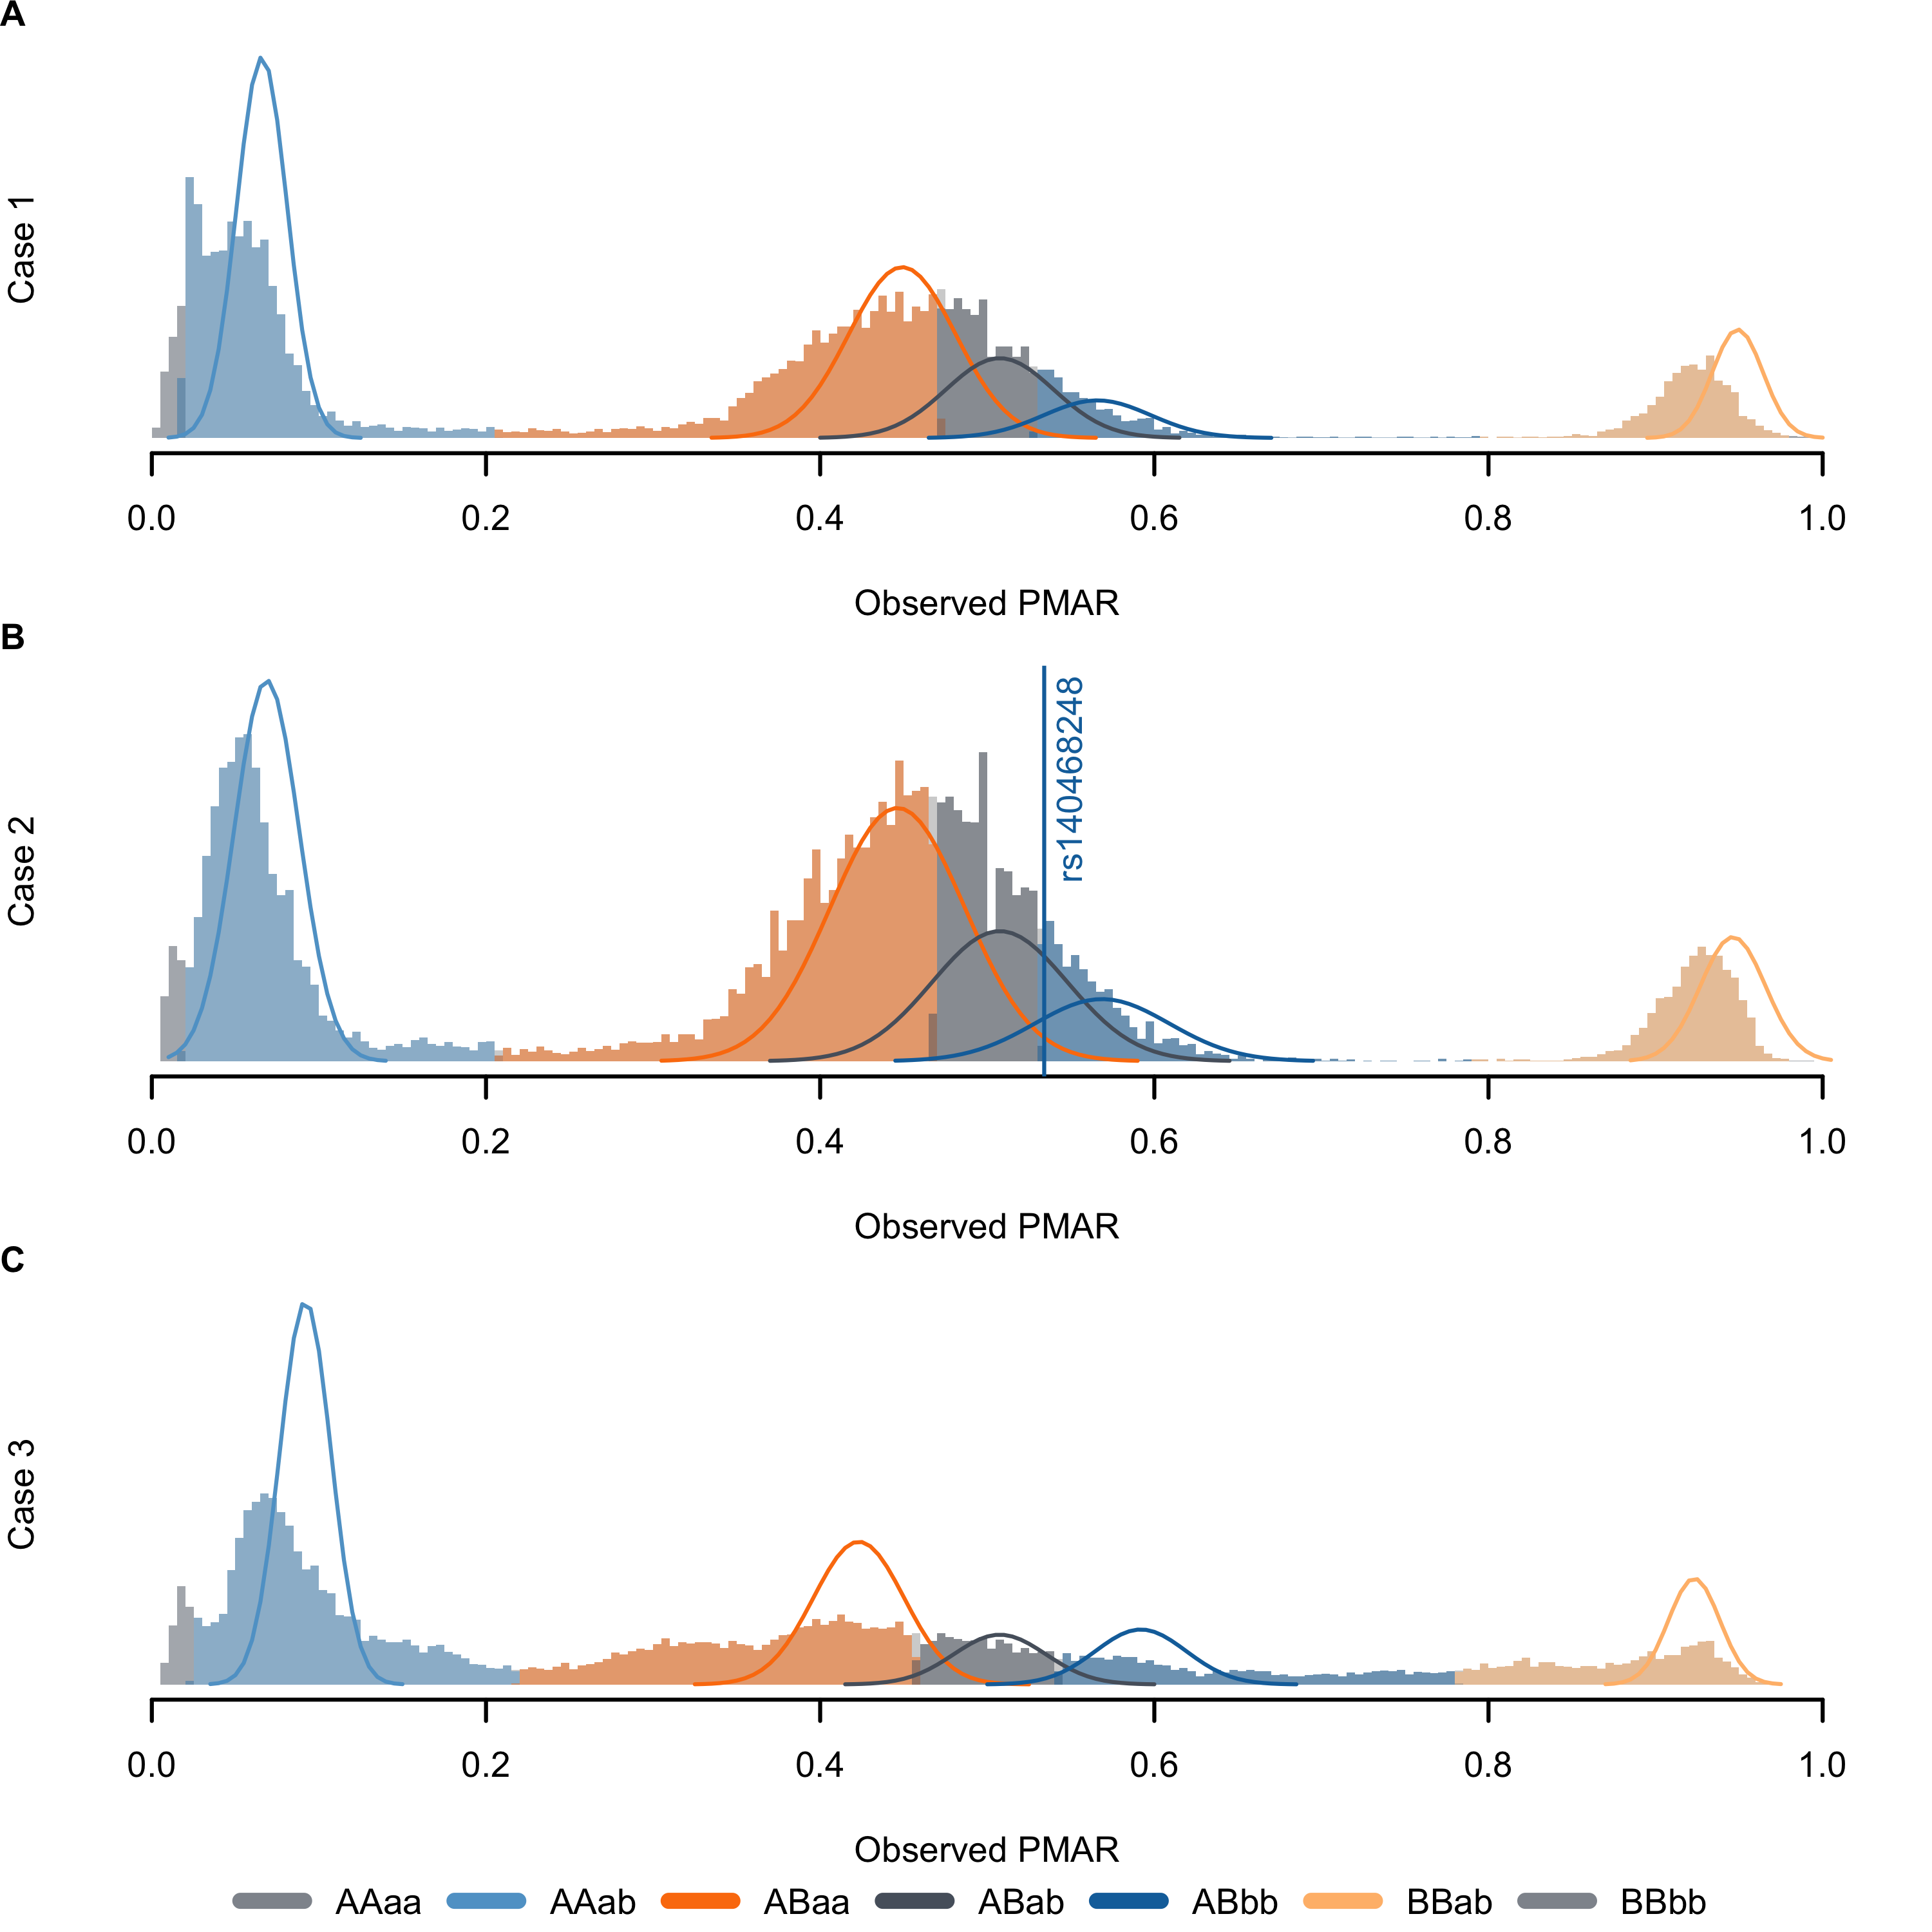
\includegraphics{DLFilerDissertation_files/figure-latex/alleleDep-1} 

}

\caption[PMAR distribution for cell-free exome sequencing cases.]{Distribution of observed proportion of minor allele reads (PMAR) values for the three cases across the possible maternal-fetal genotype pairs. Uppercase letters give the estimated maternal genotype, lowercase letters give the estimated fetal genotype; `A/a' indicates the reference allele, `B/b' indicates the alternate allele. Solid lines show the normal approximation for the theoretical distribution of binomial probabilities, given the frequency of the estimated genotypes. The vertical line in (B) shows the observed PMAR for the known pathogenic variant, rs140468248.}\label{fig:alleleDep}
\end{figure}





















\begin{table}

\caption[Cell-free exome sequencing case summaries]{\label{tab:caseSmry}Case summaries. GA: gestational age at the time of blood draw for cfES. FF: estimated fetal fraction. Depth: median depth used to estimate genotypes (does not include duplicated/filtered reads). \%Dup: percentage of total mapped read pairs discarded as PCR and/or optical duplicates. \%Filt: percentage of total mapped read pairs discarded for improper pairing and/or mapping quality.}
\centering
\begin{tabular}[t]{ll>{\raggedright\arraybackslash}p{10em}>{\raggedright\arraybackslash}p{10em}rrrr}
\toprule
  & GA & Clinical findings & Genetic diagnosis & FF & Dep & \%Dup & \%Filt\\
\midrule
1 & 32w2d & 5 prior pregnancies affected with X-linked recessive Menke's syndrome & Menke's syndrome; del. ATP7A exon 1 & 0.117 & 241 & 42.80 & 21.96\\
2 & 24w5d & Fetal sonogram at 21w5d showed femoral bowing with shortened length (\textless3\% for GA) bilaterally & Osteogenesis imperfecta type VIII; P3H1 c.1120G\textgreater T (rs140468248) & 0.122 & 152 & 33.32 & 22.09\\
3 & 34w0d & Fetal sonogram at 19w0d showed bilateral club foot with bilateral upper limb arthrogryposis & None, to date, despite exome and genome sequencing of newborn & 0.169 & 330 & 53.67 & 32.65\\
\bottomrule
\end{tabular}
\end{table}

In Case 3, in addition to cfES, we performed exome sequencing (ES) on fetal, maternal, and paternal samples.
Based on previous work demonstrating the differential length of maternal and fetal fragments,\textsuperscript{\protect\hyperlink{ref-chan:2004aa}{122}--\protect\hyperlink{ref-rabinowitz:2019aa}{125}} we interrogated the distribution of presumed maternal and fetal reads (Figure \ref{fig:matVsFetLen}).
We identified maternal and fetal reads by identifying sites with unique heterozygosity in the direct maternal and fetal ES results; at the informative sites, we extracted reads supporting the allele unique to the mother or fetus.
In total, we identified 654,619 maternal reads and 279,508 fetal reads.
We found, as others have, a higher proportion of fetal reads falling below 150 basepairs; however, we also observed a slightly higher proportion of longer reads, as well.





\begin{figure}

{\centering 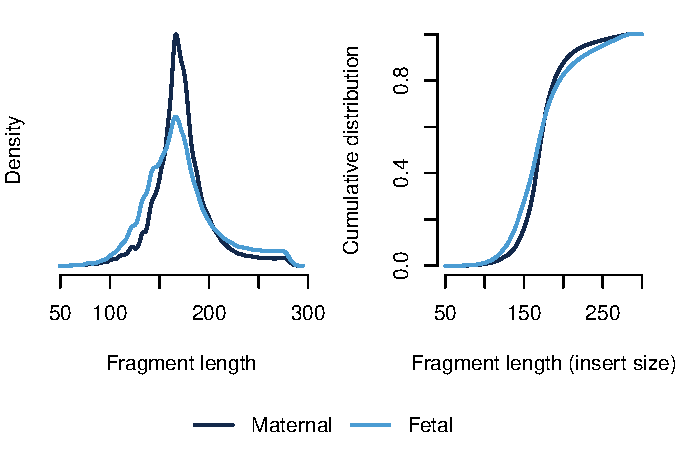
\includegraphics{DLFilerDissertation_files/figure-latex/matVsFetLen-1} 

}

\caption[Distribution of maternal versus fetal fragment length in Case 3.]{Distribution of maternal versus fetal fragment length in Case 3. (A) shows the density; (B) shows the emperic cumulative distribution. The horiztonal axis shows the fragment length (insert size taken from aligned read-pairs). Blue lines show maternal reads, orange lines show fetal reads. We only included cfES reads supporting alleles unique to the mother or fetus, as identified from the direct maternal and fetal ES.}\label{fig:matVsFetLen}
\end{figure}

Rabinowitz et al.~proposed the Hoobari method which incorporates fragment lengths into fetal genotype estimates,\textsuperscript{\protect\hyperlink{ref-rabinowitz:2019aa}{125}} finding the difference in accuracy varied from -0.25\% to 1.89\% when using versus not using fragment length in their exome analyses.
To explore the utility of correcting for fragment length in our analysis, we interrogated the PMAR as a function of the short read proportion (fraction of reads with insert sizes less than 140 basepairs; Figure \ref{fig:sratioByPmar}).
We selected 140 as the cutoff based on the Hoobari algorithm.
Overall, we found no meaningful relationship between the short read proportion and the observed PMAR and chose not to incorporate fragment length into our genotype estimates.





\begin{figure}

{\centering 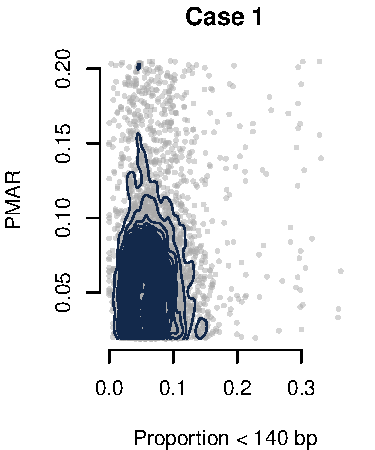
\includegraphics[width=0.33\linewidth]{DLFilerDissertation_files/figure-latex/sratioByPmar-1} 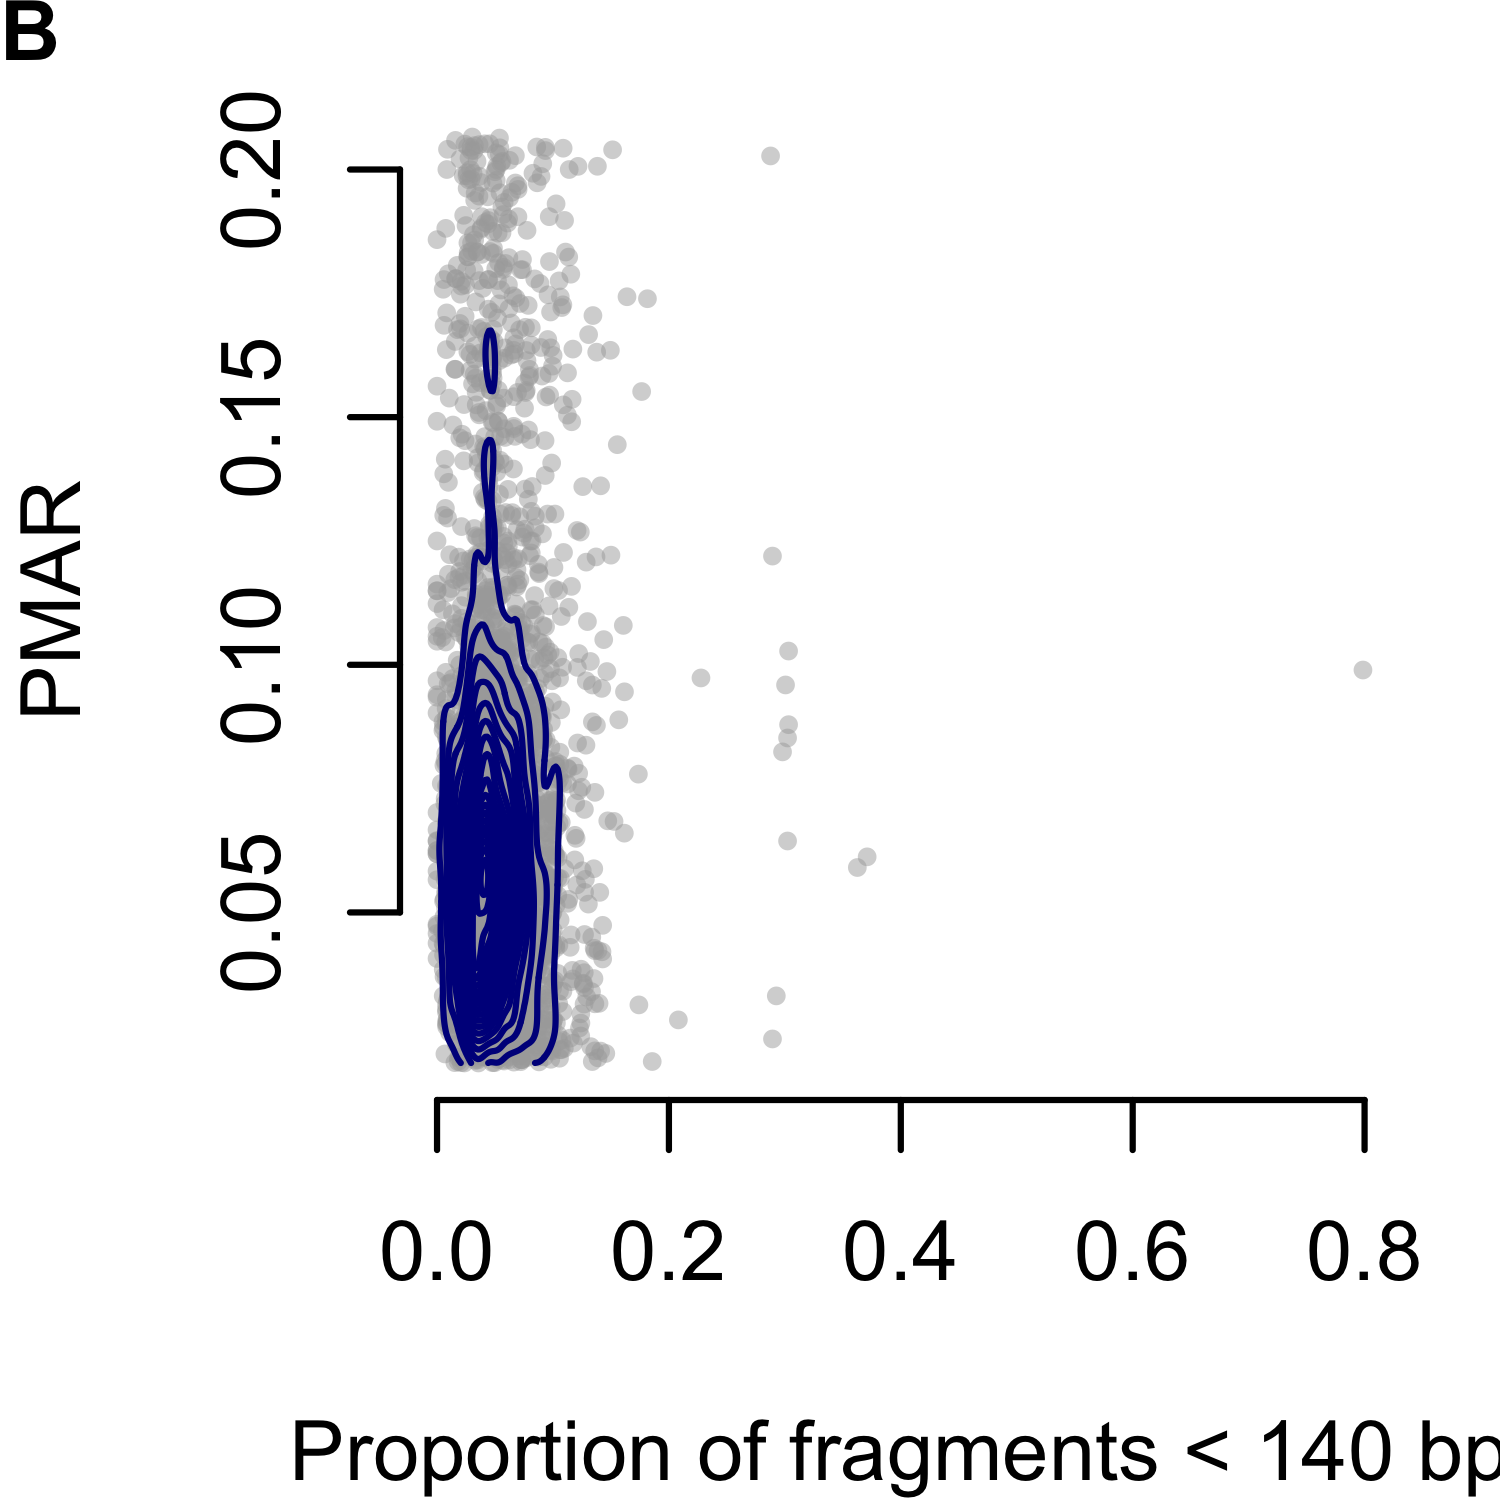
\includegraphics[width=0.33\linewidth]{DLFilerDissertation_files/figure-latex/sratioByPmar-2} 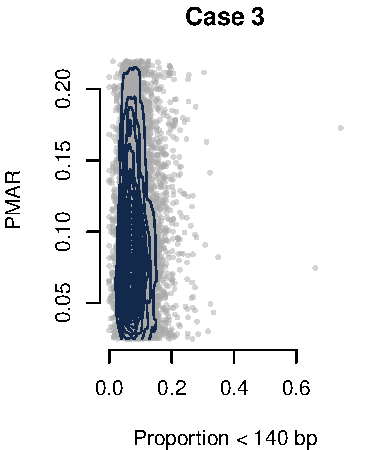
\includegraphics[width=0.33\linewidth]{DLFilerDissertation_files/figure-latex/sratioByPmar-3} 

}

\caption[Relationship between PMAR and fraction of reads \textless140 basepairs.]{Proportion of minor allele reads (PMAR) as a function of the short read proportion for genotypes estimated as `AAab.' Short reads defined as fragments less than 140 basepairs. (A-C) show Cases 1 to 3, respectively. Gray points show the individual sites; blue contour lines show the two-dimensional distribution of values.}\label{fig:sratioByPmar}
\end{figure}

Returning to Case 3, we interrogated the fetal genotyping accuracy at all sites with cell-free genotype estimates and reliable calls from the direct fetal sample.
Overall, we found a 50.91\% accuracy (Table \ref{tab:c3FetByCf}).
Table \ref{tab:c3Calls} provides the full set of maternal, fetal, and cell-free calls.





\begin{table}

\caption[Case 3 fetal versus cell-free genotype calls.]{\label{tab:c3FetByCf}Case 3 fetal versus cell-free genotype calls. `0' represents the major allele; `1' represents the minor allele. Sites with cell-free estimates and reliable direct fetal calls included (reliable defied as passing all quality checks and having a total sequencing depth greater than 30).}
\centering
\begin{tabular}[t]{llrrr}
\toprule
\multicolumn{2}{c}{ } & \multicolumn{3}{c}{Cell-free} \\
\cmidrule(l{3pt}r{3pt}){3-5}
  &   & 0/0 & 0/1 & 1/1\\
\midrule
 & 0/0 & 1,063 & 1,857 & 9\\
\cmidrule{2-5}
 & 0/1 & 3,598 & 7,079 & 1,454\\
\cmidrule{2-5}
\multirow{-3}{*}{\raggedright\arraybackslash Fetal} & 1/1 & 76 & 2,197 & 1,391\\
\bottomrule
\end{tabular}
\end{table}



\begin{table}

\caption[Maternal, fetal, and cell-free genotype calls.]{\label{tab:c3Calls}Maternal, fetal, and cell-free genotype calls. `0' represents the major allele; `1' represents the minor allele. Sites with cell-free estimates and reliable direct fetal calls included (reliable defied as passing all quality checks and having a total sequencing depth greater than 30).}
\centering
\begin{tabular}[t]{lllr}
\toprule
Maternal & Fetal & Cell-free & N\\
\midrule
 &  & 0/0 & 468\\
\cmidrule{3-4}
 & \multirow{-2}{*}{\raggedright\arraybackslash 0/0} & 0/1 & 1,159\\
\cmidrule{2-4}
 &  & 0/0 & 64\\
\cmidrule{3-4}
 & \multirow{-2}{*}{\raggedright\arraybackslash 0/1} & 0/1 & 352\\
\cmidrule{2-4}
 &  & 0/0 & 1\\
\cmidrule{3-4}
\multirow{-6}{*}{\raggedright\arraybackslash 0/0} & \multirow{-2}{*}{\raggedright\arraybackslash 1/1} & 0/1 & 2\\
\cmidrule{1-4}
 &  & 0/0 & 387\\
\cmidrule{3-4}
 &  & 0/1 & 107\\
\cmidrule{3-4}
 & \multirow{-3}{*}{\raggedright\arraybackslash 0/0} & 1/1 & 6\\
\cmidrule{2-4}
 &  & 0/0 & 3,072\\
\cmidrule{3-4}
 &  & 0/1 & 1,967\\
\cmidrule{3-4}
 & \multirow{-3}{*}{\raggedright\arraybackslash 0/1} & 1/1 & 713\\
\cmidrule{2-4}
 &  & 0/0 & 68\\
\cmidrule{3-4}
 &  & 0/1 & 458\\
\cmidrule{3-4}
\multirow{-9}{*}{\raggedright\arraybackslash 0/1} & \multirow{-3}{*}{\raggedright\arraybackslash 1/1} & 1/1 & 1,291\\
\cmidrule{1-4}
 &  & 0/1 & 1\\
\cmidrule{3-4}
 & \multirow{-2}{*}{\raggedright\arraybackslash 0/0} & 1/1 & 2\\
\cmidrule{2-4}
 &  & 0/0 & 3\\
\cmidrule{3-4}
 &  & 0/1 & 1,308\\
\cmidrule{3-4}
 & \multirow{-3}{*}{\raggedright\arraybackslash 0/1} & 1/1 & 648\\
\cmidrule{2-4}
 &  & 0/1 & 1,601\\
\cmidrule{3-4}
\multirow{-7}{*}{\raggedright\arraybackslash 1/1} & \multirow{-2}{*}{\raggedright\arraybackslash 1/1} & 1/1 & 23\\
\bottomrule
\end{tabular}
\end{table}

\hypertarget{discussion-1}{%
\section{Discussion}\label{discussion-1}}

Without the ability to reliably exclude maternal DNA fragments, noninvasive sequencing-based methods to genotype the fetus either require additional sequencing of parental samples or distinguishing genotypes by the proportion of minor allele reads (PMAR).
Here, we make no attempt to utilize parental genetic information and demonstrate the difficulty of inferring the genotypes directly from the PMAR.
We model the PMAR as a binomial proportion; given the fetal fraction, one can prove the true PMAR defines the maternal and fetal genotypes (supplemental document).

The theoretical bounds of the binomial distribution, therefore, confine our ability to discriminate maternal-fetal genotypes.
Using the normal approximation for the binomial variance (valid when the number of observations, i.e.~sequencing depth, times the binomial proportion, i.e.~PMAR, is greater than 10), we can clearly explain the poor results we observed (Figures \ref{fig:binCI} and \ref{fig:binWeitzman}).
At sequencing depths up to 500x, the 95\% confidence intervals on PMAR distributions still overlap for fetal fractions up to roughly 0.17 (Figure \ref{fig:binCI}).
When we calculate the degree of distribution overlap (a proxy for classification error rate), we see required sequencing depths in excess of 8,000x for low fetal fraction samples (Figure \ref{fig:binWeitzman}).
We, therefore, cannot expect cell-free sequencing to reliably differentiate genotypes without substantially higher depth or additional genetic information.
No amount of cleverness in the analysis can overcome the fundamental variance bounds when estimating binomial proportions.





\begin{figure}

{\centering 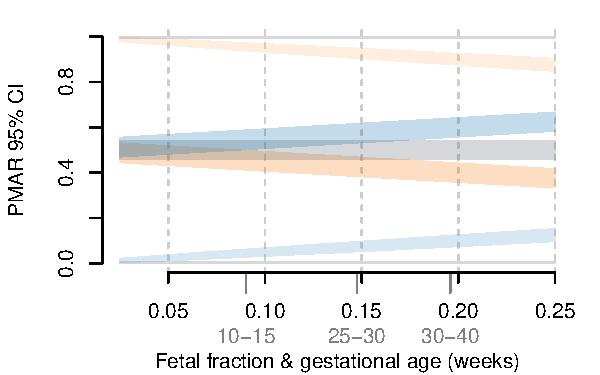
\includegraphics{DLFilerDissertation_files/figure-latex/binCI-1} 

}

\caption[95\% confidence intervals on the binomial proportions for possible maternal-fetal genotype pairs.]{95\% confidence intervals on the binomial proportions for possible maternal-fetal genotype pairs across increasing fetal fractions. Confidence intervals represent a sequencing depth of 500x. Average fetal fractions by gestational age (in weeks) given in light gray.\textsuperscript{\protect\hyperlink{ref-kinnings:2015aa}{126}}}\label{fig:binCI}
\end{figure}





\begin{figure}

{\centering 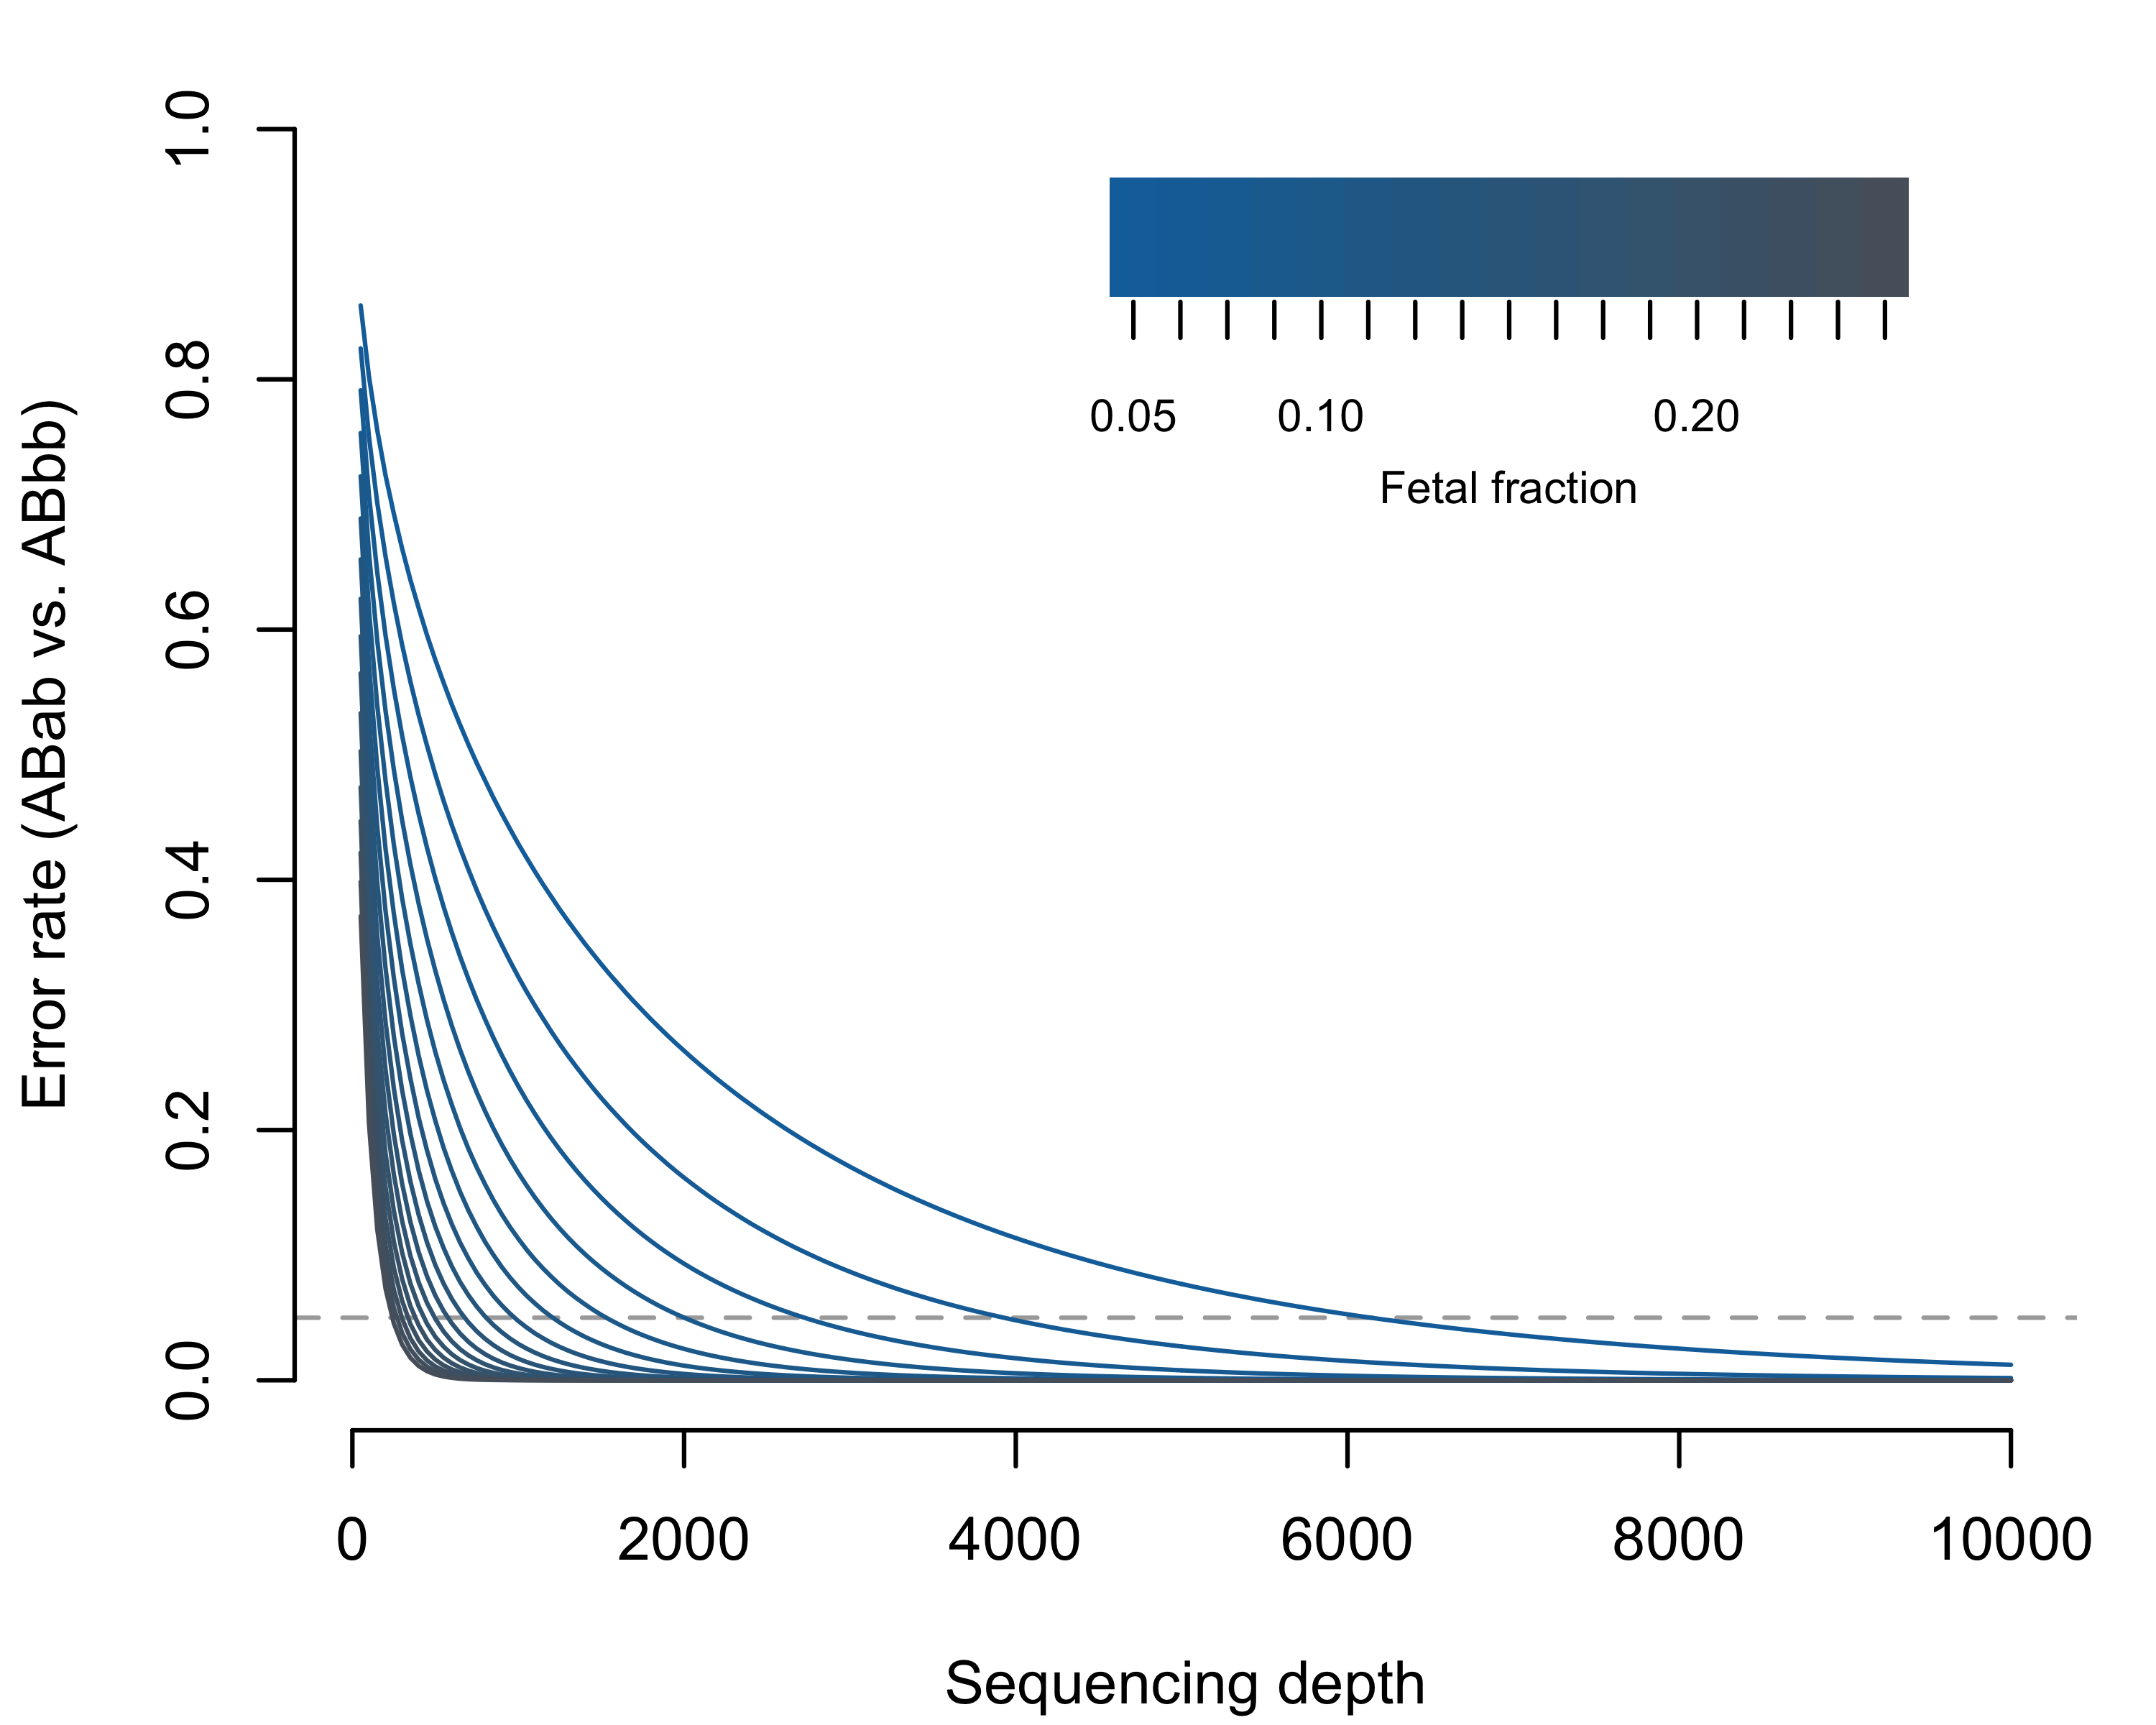
\includegraphics{DLFilerDissertation_files/figure-latex/binWeitzman-1} 

}

\caption[(ref:binWeitzmanScap)]{Expected misclassification rate (Weitzman overlapping coefficient; i.e.~the area of overlapping distributions in Figure \ref{fig:binCI}) considering ABab versus ABbb as a function of sequencing depth and fetal fraction. The dashed horizontal line shows 5\% error. The theoretical error rates for ABab vs ABaa are symmetric and equal; however, the frequency of errors will depend on the population frequency of the reference versus alternate allele.}\label{fig:binWeitzman}
\end{figure}

The sequencing herein suffers from three problems: (1) inadequate sequencing depth; (2) biased PMAR values from the removal of duplicate reads; (3) errors in sequencing and/or PCR.
We have already illustrated the inadequate depth, but emphasize that the theoretical results we present speak to the final depths (not the raw sequencing depth).
In our three cases, we excluded over half the reads taken off the sequencer due to sequencing quality thresholds (Table \ref{tab:caseSmry}).
We observe the evidence of problems (2) and (3) by observing the high proportion of both duplicate reads and PMAR values outside the theoretic distributions.
Additionally, we observed very poor accuracy in the Case 3 genotype estimates.

Typical sequencing workflows start with randomly fragmenting DNA molecules to build sequencing libraries.
Standard bioinformatic practices suggest we remove read-pairs with identical endpoints, because the duplicate read-pairs more likely represent PCR amplification of a single molecule than two molecules with the same fragmentation.
Cell-free DNA molecules are shorter than nuclear DNA, not requiring manual fragmentation, and have a non-random distribution of endpoints.\textsuperscript{\protect\hyperlink{ref-chan:2016aa}{123}}
Therefore, compared to standard sequencing libraries, the likelihood of observing true duplicates in cell-free libraries increases and we cannot necessarily assume duplicates represent PCR amplification.
However, for this work we have no way of differentiating reads representing true duplicate molecules versus PCR duplicates and thus excluded duplicate reads from our analysis.

Assuming adequate depth and appropriate handling of duplicate reads and sequencing errors, incorporating the fragment length into the statistical model may prove more beneficial.
The high variability of the binomial distribution for small \(n\) obfuscates any meaningful relationship between fragment length and PMAR in our data.
We reiterate, however, incorporating fragment length may give better estimates of the binomial proportion but cannot decrease variance beyond the distribution bounds.

To solve the above issues, we advocate a more targeted approach with much greater sequencing depth and unique molecular identifiers.
Unique molecular identifiers allow identification of sequencing errors and differentiate true versus artifactual duplicate reads.
Given the depth requirements for estimating fetal genotypes by the PMAR, and the challenge of variants of uncertain clinical significance, we advocate against broad sequencing modalities on noninvasive samples.
Recognizing that all capture methods introduce bias in the relative sequencing efficiency of different targeted regions,\textsuperscript{\protect\hyperlink{ref-seaby:2016aa}{120}} the sequencing depths needed for noninvasive fetal genotyping necessitate a targeted approach.
Despite the challenges raised by this work, we believe assessing hundreds to thousands of basepairs, rather than the tens of millions targeted in ES, will prove economical and clinically reliable.
Doing so, we hope, will foster population-level screening for Mendelian disorders during the prenatal period and, ultimately, unlock new avenues in the treatment of these disorders.

\backmatter

\setlength{\parindent}{0ex}
\cleardoublepage
\phantomsection
\addcontentsline{toc}{chapter}{REFERENCES}
\myonein{REFERENCES}

\hypertarget{refs}{}
\leavevmode\hypertarget{ref-mendel:1866aa}{}%
1. Mendel G. Versuche über pflanzenhybriden. \emph{Verh Naturf Ver Brünn}. 1866;4:3---47.

\leavevmode\hypertarget{ref-miescher:1871aa}{}%
2. Miescher F. Über die chemische zusammensetzung der eiterzellen. \emph{Hoppe-Seyler's Med Chem Unters}. 1871;4:441-460.

\leavevmode\hypertarget{ref-miescher:1874aa}{}%
3. Miescher F. Das protamin, eine neue organische basis aus den samenfäden des rheinlachses. \emph{Ber Deutsch Chem Ges}. 1874;7:376---379.

\leavevmode\hypertarget{ref-miescher:1874ab}{}%
4. Miescher F. Die spermatozoen einiger wilbertiere. \emph{Ein Beitrag zur histochemie Verh Naturf Ges}. 1874;6:138---208.

\leavevmode\hypertarget{ref-kossel:1893aa}{}%
5. Kossel A, Neumann A. Über das thymin, ein spaltungsprodukt der nukleinsäure. \emph{Ber Deutsch Chem Ges}. 1893;26:2753---2756.

\leavevmode\hypertarget{ref-flemming:1878aa}{}%
6. Flemming W. Zur kenntniss der zelle und ihrer theilungs-erscheinungen. \emph{Schriften des Naturwissenschaftlichen Vereins für Schleswig-Holstein}. 1878;3:23---27.

\leavevmode\hypertarget{ref-boveri:1902aa}{}%
7. Boveri TH. Über mehrpolige mitosen als mittel zur analyse des zellkerns. \emph{Verh Phys Med Ges Vürzb}. 1902;35:60-90.

\leavevmode\hypertarget{ref-boveri:1903aa}{}%
8. Boveri TH. Über die konstitution der chromatischen kernsubstanz. \emph{Verh Deutsch Zool Ges Würzb}. 1903;13(10--33).

\leavevmode\hypertarget{ref-sutton:1903aa}{}%
9. Sutton WS. The chromosomes in heredity. \emph{Biol Bull (Woods Hole)}. 1903;4:231-251.

\leavevmode\hypertarget{ref-avery:1944aa}{}%
10. Avery OT, Macleod CM, McCarty M. STUDIES on the chemical nature of the substance inducing transformation of pneumococcal types : INDUCTION of transformation by a desoxyribonucleic acid fraction isolated from pneumococcus type iii. \emph{J Exp Med}. 79(2):137-158.

\leavevmode\hypertarget{ref-chargaff:1949aa}{}%
11. Chargaff E, Vischer E, Doniger R, Green C, Misani F. The composition of the desoxypentose nucleic acids of thymus and spleen. \emph{J Biol Chem}. 177(1):405-416.

\leavevmode\hypertarget{ref-franklin:1953aa}{}%
12. FRANKLIN RE, GOSLING RG. Molecular configuration in sodium thymonucleate. \emph{Nature}. 171(4356):740-741.

\leavevmode\hypertarget{ref-watson:1953aa}{}%
13. WATSON JD, CRICK FH. Molecular structure of nucleic acids; a structure for deoxyribose nucleic acid. \emph{Nature}. 171(4356):737-738.

\leavevmode\hypertarget{ref-crick:1958aa}{}%
14. CRICK FH. On protein synthesis. \emph{Symp Soc Exp Biol}. 1958;12:138-163.

\leavevmode\hypertarget{ref-crick:1970aa}{}%
15. Crick F. Central dogma of molecular biology. \emph{Nature}. 227(5258):561-563.

\leavevmode\hypertarget{ref-tjio:1956aa}{}%
16. TJIO JH, LEVAN A. THE chromosome number of man. \emph{Hereditas}. 1956;42(1‐2):1-6.

\leavevmode\hypertarget{ref-lander:2001aa}{}%
17. Lander ES, Linton LM, Birren B, et al. Initial sequencing and analysis of the human genome. \emph{Nature}. 409(6822):860-921.

\leavevmode\hypertarget{ref-gu:2008aa}{}%
18. Gu W, Zhang F, Lupski JR. Mechanisms for human genomic rearrangements. \emph{Pathogenetics}. 1(1):4.

\leavevmode\hypertarget{ref-sanger:1975aa}{}%
19. Sanger F, Coulson AR. A rapid method for determining sequences in dna by primed synthesis with dna polymerase. \emph{J Mol Biol}. 94(3):441-448.

\leavevmode\hypertarget{ref-maxam:1977aa}{}%
20. Maxam AM, Gilbert W. A new method for sequencing dna. \emph{Proc Natl Acad Sci U S A}. 74(2):560-564.

\leavevmode\hypertarget{ref-sanger:1977aa}{}%
21. Sanger F, Nicklen S, Coulson AR. DNA sequencing with chain-terminating inhibitors. \emph{Proc Natl Acad Sci U S A}. 74(12):5463-5467.

\leavevmode\hypertarget{ref-nyren:1985aa}{}%
22. Nyrén P, Lundin A. Enzymatic method for continuous monitoring of inorganic pyrophosphate synthesis. \emph{Anal Biochem}. 151(2):504-509.

\leavevmode\hypertarget{ref-ronaghi:1998aa}{}%
23. Ronaghi M, Uhlén M, Nyrén P. A sequencing method based on real-time pyrophosphate. \emph{Science}. 281(5375):363, 365.

\leavevmode\hypertarget{ref-li:2003aa}{}%
24. Li Z, Bai X, Ruparel H, Kim S, Turro NJ, Ju J. A photocleavable fluorescent nucleotide for dna sequencing and analysis. \emph{Proc Natl Acad Sci U S A}. 100(2):414-419.

\leavevmode\hypertarget{ref-fedurco:2006aa}{}%
25. Fedurco M, Romieu A, Williams S, Lawrence I, Turcatti G. BTA, a novel reagent for dna attachment on glass and efficient generation of solid-phase amplified dna colonies. \emph{Nucleic Acids Res}. 34(3):e22.

\leavevmode\hypertarget{ref-turcatti:2008aa}{}%
26. Turcatti G, Romieu A, Fedurco M, Tairi A-P. A new class of cleavable fluorescent nucleotides: Synthesis and optimization as reversible terminators for dna sequencing by synthesis. \emph{Nucleic Acids Res}. 36(4):e25.

\leavevmode\hypertarget{ref-pearson:1988aa}{}%
27. Pearson WR, Lipman DJ. Improved tools for biological sequence comparison. \emph{Proc Natl Acad Sci U S A}. 85(8):2444-2448.

\leavevmode\hypertarget{ref-cock:2010aa}{}%
28. Cock PJA, Fields CJ, Goto N, Heuer ML, Rice PM. The sanger fastq file format for sequences with quality scores, and the solexa/illumina fastq variants. \emph{Nucleic Acids Res}. 38(6):1767-1771.

\leavevmode\hypertarget{ref-li:2009aa}{}%
29. Li H, Handsaker B, Wysoker A, et al. The sequence alignment/map format and samtools. \emph{Bioinformatics}. 25(16):2078-2079.

\leavevmode\hypertarget{ref-smith:1981aa}{}%
30. Smith TF, Waterman MS. Identification of common molecular subsequences. \emph{J Mol Biol}. 147(1):195-197.

\leavevmode\hypertarget{ref-needleman:1970aa}{}%
31. Needleman SB, Wunsch CD. A general method applicable to the search for similarities in the amino acid sequence of two proteins. \emph{J Mol Biol}. 48(3):443-453.

\leavevmode\hypertarget{ref-altschul:1990aa}{}%
32. Altschul SF, Gish W, Miller W, Myers EW, Lipman DJ. Basic local alignment search tool. \emph{J Mol Biol}. 215(3):403-410.

\leavevmode\hypertarget{ref-li:2010aa}{}%
33. Li H, Homer N. A survey of sequence alignment algorithms for next-generation sequencing. \emph{Brief Bioinform}. 11(5):473-483.

\leavevmode\hypertarget{ref-burrows:1994aa}{}%
34. Burrows M, Wheeler DJ. \emph{A Block-Sorting Lossless Data Compression Algorithm}.; 1994.

\leavevmode\hypertarget{ref-lam:2008aa}{}%
35. Lam TW, Sung WK, Tam SL, Wong CK, Yiu SM. Compressed indexing and local alignment of dna. \emph{Bioinformatics}. 24(6):791-797.

\leavevmode\hypertarget{ref-li:2010ab}{}%
36. Li H, Durbin R. Fast and accurate long-read alignment with burrows-wheeler transform. \emph{Bioinformatics}. 26(5):589-595.

\leavevmode\hypertarget{ref-mckenna:2010aa}{}%
37. McKenna A, Hanna M, Banks E, et al. The genome analysis toolkit: A mapreduce framework for analyzing next-generation dna sequencing data. \emph{Genome Res}. 20(9):1297-1303.

\leavevmode\hypertarget{ref-depristo:2011aa}{}%
38. DePristo MA, Banks E, Poplin R, et al. A framework for variation discovery and genotyping using next-generation dna sequencing data. \emph{Nat Genet}. 43(5):491-498.

\leavevmode\hypertarget{ref-li:2011aa}{}%
39. Li H. A statistical framework for snp calling, mutation discovery, association mapping and population genetical parameter estimation from sequencing data. \emph{Bioinformatics}. 27(21):2987-2993.

\leavevmode\hypertarget{ref-van-der-auwera:2013aa}{}%
40. Van der Auwera GA, Carneiro MO, Hartl C, et al. From fastq data to high confidence variant calls: The genome analysis toolkit best practices pipeline. \emph{Curr Protoc Bioinformatics}. 2013;43(1110):11.10.1-11.10.33.

\leavevmode\hypertarget{ref-poplin:2018aa}{}%
41. Poplin R, Ruano-Rubio V, DePristo MA, et al. Scaling accurate genetic variant discovery to tens of thousands of samples. \emph{bioRxiv}. Published online 2018.

\leavevmode\hypertarget{ref-garrison:2012aa}{}%
42. Garrison E, Marth G. Haplotype-based variant detection from short-read sequencing. Published online 2012.

\leavevmode\hypertarget{ref-chen:2019aa}{}%
43. Chen J, Li X, Zhong H, Meng Y, Du H. Systematic comparison of germline variant calling pipelines cross multiple next-generation sequencers. \emph{Sci Rep}. 9(1):9345.

\leavevmode\hypertarget{ref-xu:2018aa}{}%
44. Xu C. A review of somatic single nucleotide variant calling algorithms for next-generation sequencing data. \emph{Comput Struct Biotechnol J}. 2018;16:15-24.

\leavevmode\hypertarget{ref-abyzov:2011aa}{}%
45. Abyzov A, Urban AE, Snyder M, Gerstein M. CNVnator: An approach to discover, genotype, and characterize typical and atypical cnvs from family and population genome sequencing. \emph{Genome Res}. 21(6):974-984.

\leavevmode\hypertarget{ref-plagnol:2012aa}{}%
46. Plagnol V, Curtis J, Epstein M, et al. A robust model for read count data in exome sequencing experiments and implications for copy number variant calling. \emph{Bioinformatics}. 28(21):2747-2754.

\leavevmode\hypertarget{ref-korbel:2007aa}{}%
47. Korbel JO, Urban AE, Affourtit JP, et al. Paired-end mapping reveals extensive structural variation in the human genome. \emph{Science}. 318(5849):420-426.

\leavevmode\hypertarget{ref-layer:2014aa}{}%
48. Layer RM, Chiang C, Quinlan AR, Hall IM. LUMPY: A probabilistic framework for structural variant discovery. \emph{Genome Biol}. 15(6):R84.

\leavevmode\hypertarget{ref-zhu:2012aa}{}%
49. Zhu M, Need AC, Han Y, et al. Using erds to infer copy-number variants in high-coverage genomes. \emph{Am J Hum Genet}. 91(3):408-421.

\leavevmode\hypertarget{ref-auton:2015aa}{}%
50. Auton A, Brooks LD, Durbin RM, et al. A global reference for human genetic variation. \emph{Nature}. 526(7571):68-74.

\leavevmode\hypertarget{ref-sherry:1999aa}{}%
51. Sherry ST, Ward M, Sirotkin K. DbSNP-database for single nucleotide polymorphisms and other classes of minor genetic variation. \emph{Genome Res}. 9(8):677-679.

\leavevmode\hypertarget{ref-mailman:2007aa}{}%
52. Mailman MD, Feolo M, Jin Y, et al. The ncbi dbGaP database of genotypes and phenotypes. \emph{Nat Genet}. 39(10):1181-1186.

\leavevmode\hypertarget{ref-landrum:2014aa}{}%
53. Landrum MJ, Lee JM, Riley GR, et al. ClinVar: Public archive of relationships among sequence variation and human phenotype. \emph{Nucleic Acids Res}. 42(Database issue):D980-5.

\leavevmode\hypertarget{ref-hubbard:2002aa}{}%
54. Hubbard T, Barker D, Birney E, et al. The ensembl genome database project. \emph{Nucleic Acids Res}. 30(1):38-41.

\leavevmode\hypertarget{ref-yates:2020aa}{}%
55. Yates AD, Achuthan P, Akanni W, et al. Ensembl 2020. \emph{Nucleic Acids Res}. 48(D1):D682-D688.

\leavevmode\hypertarget{ref-mclaren:2016aa}{}%
56. McLaren W, Gil L, Hunt SE, et al. The ensembl variant effect predictor. \emph{Genome Biol}. 17(1):122.

\leavevmode\hypertarget{ref-karczewski:2019aa}{}%
57. Karczewski KJ, Francioli LC, Tiao G, et al. Variation across 141,456 human exomes and genomes reveals the spectrum of loss-of-function intolerance across human protein-coding genes. \emph{bioRxiv}. Published online 2019.

\leavevmode\hypertarget{ref-adzhubei:2013aa}{}%
58. Adzhubei I, Jordan DM, Sunyaev SR. Predicting functional effect of human missense mutations using polyphen-2. \emph{Curr Protoc Hum Genet}. Chapter 7:Unit7.20.

\leavevmode\hypertarget{ref-jager:2014aa}{}%
59. Jager M, Wang K, Bauer S, Smedley D, Krawitz P, Robinson PN. Jannovar: A java library for exome annotation. \emph{Hum Mutat}. 35(5):548-555.

\leavevmode\hypertarget{ref-harper:2008aa}{}%
60. Harper PS. \emph{A Short History of Medical Genetics}. Oxford University Press USA - OSO

\leavevmode\hypertarget{ref-garrod:1902aa}{}%
61. Garrod AE. THE incidence of alkaptonuria : A study in chemical individuality. \emph{The Lancet}. 160(4137):1616-1620.

\leavevmode\hypertarget{ref-garrod:1923aa}{}%
62. Garrod AE. \emph{Inborn Errors of Metabolism}. Oxford University Press; 1923.

\leavevmode\hypertarget{ref-garrod:1931aa}{}%
63. Garrod AE. \emph{Inborn Factors of Disease: An Essay}. Clarendon Press; 1931.

\leavevmode\hypertarget{ref-rimoin:2004aa}{}%
64. Rimoin DL, Hirschhorn K. A history of medical genetics in pediatrics. \emph{Pediatr Res}. 56(1):150-159.

\leavevmode\hypertarget{ref-fisher:1919aa}{}%
65. Fisher RA. XV.---The correlation between relatives on the supposition of mendelian inheritance. \emph{Transactions of the Royal Society of Edinburgh}. 1919;52(2):399-433.

\leavevmode\hypertarget{ref-levan:1938aa}{}%
66. LEVAN A. THE effect of colchicine on root mitoses in allium. \emph{Hereditas}. 1938;24(4):471-486.

\leavevmode\hypertarget{ref-caspersson:1970aa}{}%
67. Caspersson T, Zech L, Johansson C, Modest EJ. Identification of human chromosomes by dna-binding fluorescent agents. \emph{Chromosoma}. 1970;30(2):215-227.

\leavevmode\hypertarget{ref-seabright:1971aa}{}%
68. Seabright M. A rapid banding technique for human chromosomes. \emph{Lancet}. 2(7731):971-972.

\leavevmode\hypertarget{ref-fan:1990aa}{}%
69. Fan YS, Davis LM, Shows TB. Mapping small dna sequences by fluorescence in situ hybridization directly on banded metaphase chromosomes. \emph{Proc Natl Acad Sci U S A}. 87(16):6223-6227.

\leavevmode\hypertarget{ref-danna:1971aa}{}%
70. Danna K, Nathans D. Specific cleavage of simian virus 40 dna by restriction endonuclease of hemophilus influenzae. \emph{Proc Natl Acad Sci U S A}. 68(12):2913-2917.

\leavevmode\hypertarget{ref-southern:1975aa}{}%
71. Southern EM. Detection of specific sequences among dna fragments separated by gel electrophoresis. \emph{J Mol Biol}. 98(3):503-517.

\leavevmode\hypertarget{ref-shine:1977aa}{}%
72. Shine J, Seeburg PH, Martial JA, Baxter JD, Goodman HM. Construction and analysis of recombinant dna for human chorionic somatomammotropin. \emph{Nature}. 270(5637):494-499.

\leavevmode\hypertarget{ref-botstein:1980aa}{}%
73. Botstein D, White RL, Skolnick M, Davis RW. Construction of a genetic linkage map in man using restriction fragment length polymorphisms. \emph{Am J Hum Genet}. 32(3):314-331.

\leavevmode\hypertarget{ref-mullis:1986aa}{}%
74. Mullis K, Faloona F, Scharf S, Saiki R, Horn G, Erlich H. Specific enzymatic amplification of dna in vitro: The polymerase chain reaction. \emph{Cold Spring Harb Symp Quant Biol}. 1986;51 Pt 1:263-273.

\leavevmode\hypertarget{ref-guthrie:1963aa}{}%
75. GUTHRIE R, SUSI A. A simple phenylalanine method for detecting phenylketonuria in large populations of newborn infants. \emph{Pediatrics}. 32:338-343.

\leavevmode\hypertarget{ref-jervis:1953aa}{}%
76. JERVIS GA. Phenylpyruvic oligophrenia deficiency of phenylalanine-oxidizing system. \emph{Proc Soc Exp Biol Med}. 82(3):514-515.

\leavevmode\hypertarget{ref-bickel:1953aa}{}%
77. BICKEL H, GERRARD J, HICKMANS EM. Influence of phenylalanine intake on phenylketonuria. \emph{Lancet}. 265(6790):812-813.

\leavevmode\hypertarget{ref-fuchs:1956aa}{}%
78. FUCHS F, RIIS P. Antenatal sex determination. \emph{Nature}. 177(4503):330.

\leavevmode\hypertarget{ref-steele:1966aa}{}%
79. Steele MW, Breg WRJ. Chromosome analysis of human amniotic-fluid cells. \emph{Lancet}. 1(7434):383-385.

\leavevmode\hypertarget{ref-walknowska:1969aa}{}%
80. Walknowska J, Conte FA, Grumbach MM. Practical and theoretical implications of fetal-maternal lymphocyte transfer. \emph{Lancet}. 1(7606):1119-1122.

\leavevmode\hypertarget{ref-mueller:1990aa}{}%
81. Mueller UW, Hawes CS, Wright AE, et al. Isolation of fetal trophoblast cells from peripheral blood of pregnant women. \emph{Lancet}. 336(8709):197-200.

\leavevmode\hypertarget{ref-bianchi:1990aa}{}%
82. Bianchi DW, Flint AF, Pizzimenti MF, Knoll JH, Latt SA. Isolation of fetal dna from nucleated erythrocytes in maternal blood. \emph{Proc Natl Acad Sci U S A}. 87(9):3279-3283.

\leavevmode\hypertarget{ref-lo:1997aa}{}%
83. Lo YM, Corbetta N, Chamberlain PF, et al. Presence of fetal dna in maternal plasma and serum. \emph{Lancet}. 350(9076):485-487.

\leavevmode\hypertarget{ref-scotchman:2020aa}{}%
84. Scotchman E, Chandler NJ, Mellis R, Chitty LS. Noninvasive prenatal diagnosis of single-gene diseases: The next frontier. \emph{Clin Chem}. 66(1):53-60.

\leavevmode\hypertarget{ref-marchuk:2018aa}{}%
85. Marchuk DS, Crooks K, Strande N, et al. Increasing the diagnostic yield of exome sequencing by copy number variant analysis. \emph{PLoS One}. 2018;13(12):e0209185.

\leavevmode\hypertarget{ref-retterer:2015aa}{}%
86. Retterer K, Scuffins J, Schmidt D, et al. Assessing copy number from exome sequencing and exome array cgh based on cnv spectrum in a large clinical cohort. \emph{Genet Med}. 17(8):623-629.

\leavevmode\hypertarget{ref-yao:2017aa}{}%
87. Yao R, Zhang C, Yu T, et al. Evaluation of three read-depth based cnv detection tools using whole-exome sequencing data. \emph{Mol Cytogenet}. 2017;10:30.

\leavevmode\hypertarget{ref-fromer:2012aa}{}%
88. Fromer M, Moran JL, Chambert K, et al. Discovery and statistical genotyping of copy-number variation from whole-exome sequencing depth. \emph{Am J Hum Genet}. 91(4):597-607.

\leavevmode\hypertarget{ref-jiang:2015aa}{}%
89. Jiang Y, Oldridge DA, Diskin SJ, Zhang NR. CODEX: A normalization and copy number variation detection method for whole exome sequencing. \emph{Nucleic Acids Res}. 43(6):e39.

\leavevmode\hypertarget{ref-krumm:2012aa}{}%
90. Krumm N, Sudmant PH, Ko A, et al. Copy number variation detection and genotyping from exome sequence data. \emph{Genome Res}. 22(8):1525-1532.

\leavevmode\hypertarget{ref-truty:2019aa}{}%
91. Truty R, Paul J, Kennemer M, et al. Prevalence and properties of intragenic copy-number variation in mendelian disease genes. \emph{Genet Med}. 21(1):114-123.

\leavevmode\hypertarget{ref-benjamini:2012aa}{}%
92. Benjamini Y, Speed TP. Summarizing and correcting the gc content bias in high-throughput sequencing. \emph{Nucleic Acids Res}. 40(10):e72.

\leavevmode\hypertarget{ref-kadalayil:2015aa}{}%
93. Kadalayil L, Rafiq S, Rose-Zerilli MJJ, et al. Exome sequence read depth methods for identifying copy number changes. \emph{Brief Bioinform}. 16(3):380-392.

\leavevmode\hypertarget{ref-chiang:2009aa}{}%
94. Chiang DY, Getz G, Jaffe DB, et al. High-resolution mapping of copy-number alterations with massively parallel sequencing. \emph{Nat Methods}. 6(1):99-103.

\leavevmode\hypertarget{ref-foreman:2013aa}{}%
95. Foreman AKM, Lee K, Evans JP. The NCGENES project: Exploring the new world of genome sequencing. \emph{N C Med J}. 74(6):500-504.

\leavevmode\hypertarget{ref-li:2013ab}{}%
96. Li H. Aligning sequence reads, clone sequences and assembly contigs with bwa-mem. Published online 2013.

\leavevmode\hypertarget{ref-koster:2012aa}{}%
97. Koster J, Rahmann S. Snakemake--a scalable bioinformatics workflow engine. \emph{Bioinformatics}. 28(19):2520-2522.

\leavevmode\hypertarget{ref-trost:2018aa}{}%
98. Trost B, Walker S, Wang Z, et al. A comprehensive workflow for read depth-based identification of copy-number variation from whole-genome sequence data. \emph{Am J Hum Genet}. 102(1):142-155.

\leavevmode\hypertarget{ref-yu:2013aa}{}%
99. Yu D, Huber W, Vitek O. Shrinkage estimation of dispersion in negative binomial models for rna-seq experiments with small sample size. \emph{Bioinformatics}. 29(10):1275-1282.

\leavevmode\hypertarget{ref-benjamini:1995aa}{}%
100. Benjamini Y, Hochberg Y. Controlling the false discovery rate: A practical and powerful approach to multiple testing. \emph{Journal of the Royal Statistical Society: Series B (Methodological)}. 1995;57(1):289-300.

\leavevmode\hypertarget{ref-minka:2000aa}{}%
101. Minka TP. \emph{Estimating a Dirichlet Distribution}.; 2000.

\leavevmode\hypertarget{ref-matthews:1975aa}{}%
102. Matthews BW. Comparison of the predicted and observed secondary structure of t4 phage lysozyme. \emph{Biochim Biophys Acta}. 405(2):442-451.

\leavevmode\hypertarget{ref-neiman:2012aa}{}%
103. Neiman M, Sundling S, Grönberg H, et al. Library preparation and multiplex capture for massive parallel sequencing applications made efficient and easy. \emph{PLOS ONE}. 2012;7(11):1-6.

\leavevmode\hypertarget{ref-ramos:2012aa}{}%
104. Ramos E, Levinson BT, Chasnoff S, et al. Population-based rare variant detection via pooled exome or custom hybridization capture with or without individual indexing. \emph{BMC Genomics}. 13:683.

\leavevmode\hypertarget{ref-rohland:2012aa}{}%
105. Rohland N, Reich D. Cost-effective, high-throughput dna sequencing libraries for multiplexed target capture. \emph{Genome Res}. 22(5):939-946.

\leavevmode\hypertarget{ref-wesolowska:2011aa}{}%
106. Wesolowska A, Dalgaard MD, Borst L, et al. Cost-effective multiplexing before capture allows screening of 25 000 clinically relevant snps in childhood acute lymphoblastic leukemia. \emph{Leukemia}. 25(6):1001-1006.

\leavevmode\hypertarget{ref-shearer:2012aa}{}%
107. Shearer AE, Hildebrand MS, Ravi H, et al. Pre-capture multiplexing improves efficiency and cost-effectiveness of targeted genomic enrichment. \emph{BMC Genomics}. 13:618.

\leavevmode\hypertarget{ref-mackie:2017aa}{}%
108. Mackie FL, Hemming K, Allen S, Morris RK, Kilby MD. The accuracy of cell-free fetal dna-based non-invasive prenatal testing in singleton pregnancies: A systematic review and bivariate meta-analysis. \emph{BJOG}. 124(1):32-46.

\leavevmode\hypertarget{ref-zhang:2019aa}{}%
109. Zhang J, Li J, Saucier JB, et al. Non-invasive prenatal sequencing for multiple mendelian monogenic disorders using circulating cell-free fetal dna. \emph{Nat Med}.

\leavevmode\hypertarget{ref-tsao:2019ab}{}%
110. Tsao DS, Silas S, Landry BP, et al. A novel high-throughput molecular counting method with single base-pair resolution enables accurate single-gene nipt. \emph{Sci Rep}. 9(1):14382.

\leavevmode\hypertarget{ref-lo:2010aa}{}%
111. Lo YMD, Chan KCA, Sun H, et al. Maternal plasma dna sequencing reveals the genome-wide genetic and mutational profile of the fetus. \emph{Sci Transl Med}. 2(61):61ra91.

\leavevmode\hypertarget{ref-hui:2017aa}{}%
112. Hui WWI, Jiang P, Tong YK, et al. Universal haplotype-based noninvasive prenatal testing for single gene diseases. \emph{Clin Chem}. 63(2):513-524.

\leavevmode\hypertarget{ref-jang:2018aa}{}%
113. Jang SS, Lim BC, Yoo S-K, et al. Targeted linked-read sequencing for direct haplotype phasing of maternal dmd alleles: A practical and reliable method for noninvasive prenatal diagnosis. \emph{Sci Rep}. 8(1):8678.

\leavevmode\hypertarget{ref-vermeulen:2017aa}{}%
114. Vermeulen C, Geeven G, Wit E de, et al. Sensitive monogenic noninvasive prenatal diagnosis by targeted haplotyping. \emph{Am J Hum Genet}. 101(3):326-339.

\leavevmode\hypertarget{ref-chandler:2020aa}{}%
115. Chandler NJ, Ahlfors H, Drury S, et al. Noninvasive prenatal diagnosis for cystic fibrosis: Implementation, uptake, outcome, and implications. \emph{Clin Chem}. 66(1):207-216.

\leavevmode\hypertarget{ref-salomon:2019aa}{}%
116. Salomon LJ, Sotiriadis A, Wulff CB, Odibo A, Akolekar R. Risk of miscarriage following amniocentesis or chorionic villus sampling: Systematic review of literature and updated meta-analysis. \emph{Ultrasound Obstet Gynecol}. 54(4):442-451.

\leavevmode\hypertarget{ref-fan:2012aa}{}%
117. Fan HC, Gu W, Wang J, Blumenfeld YJ, El-Sayed YY, Quake SR. Non-invasive prenatal measurement of the fetal genome. \emph{Nature}. 487(7407):320-324.

\leavevmode\hypertarget{ref-kitzman:2012aa}{}%
118. Kitzman JO, Snyder MW, Ventura M, et al. Noninvasive whole-genome sequencing of a human fetus. \emph{Sci Transl Med}. 4(137):137ra76.

\leavevmode\hypertarget{ref-snyder:2013aa}{}%
119. Snyder MW, Simmons LE, Kitzman JO, et al. Noninvasive fetal genome sequencing: A primer. \emph{Prenat Diagn}. 33(6):547-554.

\leavevmode\hypertarget{ref-seaby:2016aa}{}%
120. Seaby EG, Pengelly RJ, Ennis S. Exome sequencing explained: A practical guide to its clinical application. \emph{Brief Funct Genomics}. 15(5):374-384.

\leavevmode\hypertarget{ref-r-core-team:2019aa}{}%
121. R Core Team. \emph{R: A Language and Environment for Statistical Computing}. R Foundation for Statistical Computing; 2019.

\leavevmode\hypertarget{ref-chan:2004aa}{}%
122. Chan KCA, Zhang J, Hui ABY, et al. Size distributions of maternal and fetal dna in maternal plasma. \emph{Clin Chem}. 50(1):88-92.

\leavevmode\hypertarget{ref-chan:2016aa}{}%
123. Chan KCA, Jiang P, Sun K, et al. Second generation noninvasive fetal genome analysis reveals de novo mutations, single-base parental inheritance, and preferred dna ends. \emph{Proc Natl Acad Sci U S A}. 113(50):E8159-E8168.

\leavevmode\hypertarget{ref-jiang:2016ab}{}%
124. Jiang P, Lo YMD. The long and short of circulating cell-free dna and the ins and outs of molecular diagnostics. \emph{Trends Genet}. 32(6):360-371.

\leavevmode\hypertarget{ref-rabinowitz:2019aa}{}%
125. Rabinowitz T, Polsky A, Golan D, et al. Bayesian-based noninvasive prenatal diagnosis of single-gene disorders. \emph{Genome Res}. 29(3):428-438.

\leavevmode\hypertarget{ref-kinnings:2015aa}{}%
126. Kinnings SL, Geis JA, Almasri E, et al. Factors affecting levels of circulating cell-free fetal dna in maternal plasma and their implications for noninvasive prenatal testing. \emph{Prenat Diagn}. 35(8):816-822.

\hypertarget{appendix-appendix}{%
\appendix}


\hypertarget{r-code}{%
\chapter{R Code}\label{r-code}}

This appendix contains all of the R code to reproduce the work presented.

\begin{Shaded}
\begin{Highlighting}[]
\KeywordTok{options}\NormalTok{(}\DataTypeTok{knitr.graphics.auto_pdf =} \OtherTok{TRUE}\NormalTok{)}
\NormalTok{knitr}\OperatorTok{::}\NormalTok{opts_chunk}\OperatorTok{$}\KeywordTok{set}\NormalTok{(}
  \DataTypeTok{echo      =} \OtherTok{FALSE}\NormalTok{,}
  \DataTypeTok{warning   =} \OtherTok{FALSE}\NormalTok{,}
  \DataTypeTok{message   =} \OtherTok{FALSE}\NormalTok{,}
  \DataTypeTok{error     =} \OtherTok{FALSE}\NormalTok{,}
  \DataTypeTok{cache     =} \OtherTok{TRUE}\NormalTok{,}
  \DataTypeTok{fig.align =} \StringTok{"center"}\NormalTok{,}
  \DataTypeTok{fig.width =} \DecValTok{5}\NormalTok{,}
  \DataTypeTok{fig.height =} \DecValTok{4}\NormalTok{,}
  \DataTypeTok{dev.args =} \KeywordTok{list}\NormalTok{(}\DataTypeTok{pdf =} \KeywordTok{list}\NormalTok{(}\DataTypeTok{pointsize =} \DecValTok{10}\NormalTok{),}
                  \DataTypeTok{png =} \KeywordTok{list}\NormalTok{(}\DataTypeTok{pointsize =} \DecValTok{10}\NormalTok{)),}
  \DataTypeTok{dpi =} \DecValTok{300}
\NormalTok{)}
\NormalTok{tex  <-}\StringTok{ }\OtherTok{TRUE}
\NormalTok{docx <-}\StringTok{ }\OtherTok{FALSE}
\NormalTok{html <-}\StringTok{ }\OtherTok{FALSE}
\ControlFlowTok{if}\NormalTok{ (}\OperatorTok{!}\NormalTok{knitr}\OperatorTok{:::}\KeywordTok{is_latex_output}\NormalTok{()) \{}
\NormalTok{    tex <-}\StringTok{ }\OtherTok{FALSE}
    \ControlFlowTok{if}\NormalTok{ (knitr}\OperatorTok{:::}\KeywordTok{is_html_output}\NormalTok{()) \{}
\NormalTok{        html <-}\StringTok{ }\OtherTok{TRUE}
\NormalTok{    \} }\ControlFlowTok{else}\NormalTok{ \{}
\NormalTok{        docx <-}\StringTok{ }\OtherTok{TRUE}
\NormalTok{    \}}
\NormalTok{\}}
\KeywordTok{library}\NormalTok{(filer2020A)}
\KeywordTok{library}\NormalTok{(filer2020B)}
\KeywordTok{library}\NormalTok{(mcCNV)}
\KeywordTok{library}\NormalTok{(xtable)}
\KeywordTok{library}\NormalTok{(eulerr)}
\KeywordTok{library}\NormalTok{(dlfUtils)}
\KeywordTok{library}\NormalTok{(parallel)}
\KeywordTok{library}\NormalTok{(grid)}
\KeywordTok{library}\NormalTok{(kableExtra)}
\KeywordTok{library}\NormalTok{(MASS)}
\NormalTok{defOutWid <-}\StringTok{ }\ControlFlowTok{if}\NormalTok{ (html) }\StringTok{'70%'} \ControlFlowTok{else} \OtherTok{NULL}
\NormalTok{dblOutWid <-}\StringTok{ }\ControlFlowTok{if}\NormalTok{ (html) }\StringTok{'40%'} \ControlFlowTok{else} \StringTok{'49%'}
\KeywordTok{data}\NormalTok{(subjectMeta)}
\NormalTok{poolTbl <-}\StringTok{ }\NormalTok{subjectMeta[ ,}
\NormalTok{                       .(}\DataTypeTok{N =}\NormalTok{ .N,}
                         \DataTypeTok{medExon =} \KeywordTok{round}\NormalTok{(}\KeywordTok{median}\NormalTok{(medIntMolCount), }\DecValTok{0}\NormalTok{),}
                         \DataTypeTok{medTotal =} \KeywordTok{round}\NormalTok{(}\KeywordTok{median}\NormalTok{(totalMolCount), }\DecValTok{0}\NormalTok{),}
                         \DataTypeTok{minTotal =} \KeywordTok{min}\NormalTok{(totalMolCount),}
                         \DataTypeTok{maxTotal =} \KeywordTok{max}\NormalTok{(totalMolCount),}
                         \DataTypeTok{rsdTotal =} \KeywordTok{sd}\NormalTok{(totalMolCount)}\OperatorTok{/}\KeywordTok{mean}\NormalTok{(totalMolCount)}\OperatorTok{*}\DecValTok{100}\NormalTok{),}
\NormalTok{                       by =}\StringTok{ }\NormalTok{.(pool, capture, multiplexCapture)]}
\NormalTok{poolTbl[ , rsdTotal }\OperatorTok{:}\ErrorTok{=}\StringTok{ }\KeywordTok{round}\NormalTok{(rsdTotal, }\DecValTok{1}\NormalTok{)]}
\NormalTok{poolTbl[(}\OperatorTok{!}\NormalTok{multiplexCapture), pool }\OperatorTok{:}\ErrorTok{=}\StringTok{ }\KeywordTok{paste0}\NormalTok{(pool, }\StringTok{"$^}\CharTok{\textbackslash{}\textbackslash{}}\StringTok{dagger$"}\NormalTok{)]}
\KeywordTok{kable}\NormalTok{(poolTbl[ , .(pool, capture, N, medExon, medTotal, minTotal, maxTotal, rsdTotal)], }
      \DataTypeTok{row.names =} \OtherTok{FALSE}\NormalTok{, }
      \DataTypeTok{caption =} \StringTok{'Summary of whole-exome sequencing. ``pool'' indicates the name of the pool of samples; ``capture'' indicates the capture platform for the pool; ``N'' gives the number of samples in the pool; ``medExon'' gives the pool median of the subject median mapped molecule count per exon; ``medTotal'' gives the median by pool of total mapped molecule counts per subject; ``minTotal'' and ``maxTotal'' give the minimum and maximum total mapped molecules; ``rsdTotal'' gives the relative standard deviation (SD/mean*100) of total mapped molecules. \(^\dagger\) indicates captures were performed independently on each sample within the pool, otherwise captures were multiplexed across all samples within the pool.'}\NormalTok{,}
      \DataTypeTok{label =} \StringTok{"poolSummary"}\NormalTok{,}
      \DataTypeTok{format.args =} \KeywordTok{list}\NormalTok{(}\DataTypeTok{big.mark =} \StringTok{","}\NormalTok{, }\DataTypeTok{scientific =} \OtherTok{FALSE}\NormalTok{),}
      \DataTypeTok{booktabs =} \OtherTok{TRUE}\NormalTok{,}
      \DataTypeTok{caption.short =} \StringTok{"Summary of whole-exome sequencing for CNV project."}\NormalTok{,}
      \DataTypeTok{escape =} \OtherTok{FALSE}\NormalTok{) }\OperatorTok
\StringTok{  }\KeywordTok{kable_classic}\NormalTok{()}
\CommentTok{## Create IC pools}
\NormalTok{smplSubject <-}\StringTok{ }\ControlFlowTok{function}\NormalTok{(poolName, n) \{}
  \KeywordTok{data}\NormalTok{(subjectMeta, }\DataTypeTok{envir =} \KeywordTok{environment}\NormalTok{())}
\NormalTok{  subjectMeta[pool }\OperatorTok{==}\StringTok{ }\NormalTok{poolName, }\KeywordTok{sample}\NormalTok{(subject, n, }\DataTypeTok{replace =} \OtherTok{FALSE}\NormalTok{)]}
\NormalTok{\}}
\KeywordTok{set.seed}\NormalTok{(}\DecValTok{1234}\NormalTok{)}
\NormalTok{pools <-}\StringTok{ }\KeywordTok{c}\NormalTok{(}\KeywordTok{replicate}\NormalTok{(}\DecValTok{5}\NormalTok{, }\KeywordTok{smplSubject}\NormalTok{(}\StringTok{"NCGENES"}\NormalTok{, }\DecValTok{16}\NormalTok{), }\DataTypeTok{simplify =} \OtherTok{FALSE}\NormalTok{))}
\KeywordTok{names}\NormalTok{(pools) <-}\StringTok{ }\KeywordTok{c}\NormalTok{(}\KeywordTok{sprintf}\NormalTok{(}\StringTok{"randNCG_%d"}\NormalTok{, }\DecValTok{1}\OperatorTok{:}\DecValTok{5}\NormalTok{))}
\NormalTok{pools <-}\StringTok{ }\KeywordTok{c}\NormalTok{(pools,}
           \KeywordTok{with}\NormalTok{(subjectMeta[pool }\OperatorTok{!=}\StringTok{ "NCGENES"}\NormalTok{], }\KeywordTok{split}\NormalTok{(subject, pool)))}
\CommentTok{## Calculate mean-variance by pool}
\NormalTok{mnvr <-}\StringTok{ }\KeywordTok{mclapply}\NormalTok{(pools, subsetCounts, }\DataTypeTok{mc.cores =} \KeywordTok{length}\NormalTok{(pools))}
\NormalTok{mnvr <-}\StringTok{ }\KeywordTok{mclapply}\NormalTok{(mnvr, calcIntStats, }\DataTypeTok{mc.cores =} \KeywordTok{length}\NormalTok{(mnvr))}
\ControlFlowTok{for}\NormalTok{ (i }\ControlFlowTok{in} \KeywordTok{seq_along}\NormalTok{(mnvr)) \{}
\NormalTok{  mnvr[[i]][ , pool }\OperatorTok{:}\ErrorTok{=}\StringTok{ }\KeywordTok{names}\NormalTok{(mnvr)[i]]}
\NormalTok{\}}
\NormalTok{mnvr <-}\StringTok{ }\KeywordTok{rbindlist}\NormalTok{(mnvr)}
\KeywordTok{setkey}\NormalTok{(mnvr, pool); }\KeywordTok{setcolorder}\NormalTok{(mnvr)}

\CommentTok{## Estimate alpha0}
\NormalTok{alpha0 <-}\StringTok{ }\KeywordTok{mclapply}\NormalTok{(pools, estAlpha0, }\DataTypeTok{mc.cores =} \KeywordTok{length}\NormalTok{(pools))}
\NormalTok{a0tbl <-}\StringTok{ }\KeywordTok{data.table}\NormalTok{(}\DataTypeTok{pool =} \KeywordTok{names}\NormalTok{(alpha0),}
                    \DataTypeTok{a0 =} \KeywordTok{sapply}\NormalTok{(alpha0, }\StringTok{"[["}\NormalTok{, }\StringTok{"a0"}\NormalTok{),}
                    \DataTypeTok{N =} \KeywordTok{sapply}\NormalTok{(alpha0, }\StringTok{"[["}\NormalTok{, }\StringTok{"N"}\NormalTok{))}
\NormalTok{a0tbl[ , aMn }\OperatorTok{:}\ErrorTok{=}\StringTok{ }\NormalTok{a0}\OperatorTok{/}\NormalTok{N]}
\NormalTok{calcRange <-}\StringTok{ }\ControlFlowTok{function}\NormalTok{(x) \{}
\NormalTok{  subjectMeta[subject }\OperatorTok\StringTok{ }\NormalTok{x,}
\NormalTok{              .(}\DataTypeTok{mnCount =} \KeywordTok{min}\NormalTok{(totalMolCount),}
                \DataTypeTok{mdCount =} \KeywordTok{median}\NormalTok{(totalMolCount),}
                \DataTypeTok{mxCount =} \KeywordTok{max}\NormalTok{(totalMolCount),}
                \DataTypeTok{rsCount =} \KeywordTok{sd}\NormalTok{(totalMolCount)}\OperatorTok{/}\KeywordTok{mean}\NormalTok{(totalMolCount)}\OperatorTok{*}\DecValTok{100}\NormalTok{)]}
\NormalTok{\}}
\NormalTok{poolCts <-}\StringTok{ }\KeywordTok{lapply}\NormalTok{(pools, calcRange)}
\NormalTok{poolCts <-}\StringTok{ }\KeywordTok{lapply}\NormalTok{(}\KeywordTok{names}\NormalTok{(poolCts), }\ControlFlowTok{function}\NormalTok{(x) poolCts[[x]][ , }\DataTypeTok{pool :=}\NormalTok{ x])}
\NormalTok{poolCts <-}\StringTok{ }\KeywordTok{rbindlist}\NormalTok{(poolCts)}
\NormalTok{a0tbl <-}\StringTok{ }\KeywordTok{merge}\NormalTok{(a0tbl, poolCts)}
\NormalTok{a0tbl[ , mc }\OperatorTok{:}\ErrorTok{=}\StringTok{ }\OperatorTok{!}\KeywordTok{grepl}\NormalTok{(}\StringTok{"IDT-IC|rand"}\NormalTok{, pool)]}
\NormalTok{a0tbl[ , idt }\OperatorTok{:}\ErrorTok{=}\StringTok{ }\KeywordTok{grepl}\NormalTok{(}\StringTok{"IDT"}\NormalTok{, pool)]}
\KeywordTok{pltAlpha0}\NormalTok{(a0tbl)}
\NormalTok{aglPools <-}\StringTok{ }\KeywordTok{c}\NormalTok{(}\KeywordTok{sprintf}\NormalTok{(}\StringTok{"randNCG_%d"}\NormalTok{, }\DecValTok{1}\OperatorTok{:}\DecValTok{5}\NormalTok{), }\StringTok{"Pool1"}\NormalTok{, }\StringTok{"Pool2"}\NormalTok{, }\StringTok{"WGS"}\NormalTok{, }\StringTok{"SMA1"}\NormalTok{, }\StringTok{"SMA2"}\NormalTok{)}
\KeywordTok{with}\NormalTok{(mnvr[pool }\OperatorTok\StringTok{ }\NormalTok{aglPools], \{}
  \KeywordTok{pltMnVrCont}\NormalTok{(}\DataTypeTok{dat =} \KeywordTok{as.data.table}\NormalTok{(}\KeywordTok{as.list}\NormalTok{(}\KeywordTok{environment}\NormalTok{())),}
              \DataTypeTok{grpVec =} \KeywordTok{factor}\NormalTok{(pool, }\DataTypeTok{levels =}\NormalTok{ aglPools),}
              \DataTypeTok{colVec =} \KeywordTok{c}\NormalTok{(}\KeywordTok{rep}\NormalTok{(}\StringTok{'darkblue'}\NormalTok{, }\DecValTok{5}\NormalTok{), }\KeywordTok{rep}\NormalTok{(}\StringTok{'darkorange'}\NormalTok{, }\DecValTok{5}\NormalTok{)),}
              \DataTypeTok{lgnd =} \OtherTok{FALSE}\NormalTok{)}
\NormalTok{\})}
\NormalTok{idtPools <-}\StringTok{ }\KeywordTok{c}\NormalTok{(}\StringTok{"IDT-MC"}\NormalTok{, }\StringTok{"IDT-IC"}\NormalTok{, }\StringTok{"IDT-RR"}\NormalTok{)}
\KeywordTok{with}\NormalTok{(mnvr[pool }\OperatorTok\StringTok{ }\NormalTok{idtPools], \{}
  \KeywordTok{pltMnVrCont}\NormalTok{(}\DataTypeTok{dat =} \KeywordTok{as.data.table}\NormalTok{(}\KeywordTok{as.list}\NormalTok{(}\KeywordTok{environment}\NormalTok{())),}
              \DataTypeTok{grpVec =} \KeywordTok{factor}\NormalTok{(pool, }\DataTypeTok{levels =}\NormalTok{ idtPools),}
              \DataTypeTok{colVec =} \KeywordTok{c}\NormalTok{(}\StringTok{"darkorange"}\NormalTok{, }\StringTok{"darkblue"}\NormalTok{, }\StringTok{"darkorange"}\NormalTok{),}
              \DataTypeTok{lgnd =} \OtherTok{FALSE}\NormalTok{)}
\NormalTok{\})}
\KeywordTok{with}\NormalTok{(mnvr[pool }\OperatorTok\StringTok{ }\KeywordTok{c}\NormalTok{(}\StringTok{"WGS"}\NormalTok{, }\StringTok{"IDT-RR"}\NormalTok{)], \{}
  \KeywordTok{pltMnVrCont}\NormalTok{(}\DataTypeTok{dat =} \KeywordTok{as.data.table}\NormalTok{(}\KeywordTok{as.list}\NormalTok{(}\KeywordTok{environment}\NormalTok{())),}
              \DataTypeTok{grpVec =} \KeywordTok{factor}\NormalTok{(pool, }\DataTypeTok{levels =} \KeywordTok{c}\NormalTok{(}\StringTok{"WGS"}\NormalTok{, }\StringTok{"IDT-RR"}\NormalTok{)),}
              \DataTypeTok{colVec =} \KeywordTok{c}\NormalTok{(}\StringTok{"darkblue"}\NormalTok{, }\StringTok{"darkorange"}\NormalTok{))}
\NormalTok{\})}
\KeywordTok{pltSubjectStatByPool}\NormalTok{(}\StringTok{"medIntMolCount"}\NormalTok{, }\DataTypeTok{ylab =} \StringTok{"Median count per exon"}\NormalTok{)}
\KeywordTok{pltSubjectStatByPool}\NormalTok{(}\StringTok{"nSelected"}\NormalTok{, }\DataTypeTok{ylab =} \StringTok{"Number of controls selected"}\NormalTok{)}
\KeywordTok{pltSubjectStatByPool}\NormalTok{(}\StringTok{"propSelected"}\NormalTok{, }\DataTypeTok{ylab =} \StringTok{"Proportion of controls selected"}\NormalTok{)}
\KeywordTok{pltSubjectStatByPool}\NormalTok{(}\StringTok{"overallPhi"}\NormalTok{, }\DataTypeTok{ylab =} \StringTok{"Overdispersion (phi)"}\NormalTok{)}
\KeywordTok{setkey}\NormalTok{(subjectMeta, subject)}
\KeywordTok{data}\NormalTok{(subjectCorr)}
\KeywordTok{setkey}\NormalTok{(subjectCorr, subject)}
\NormalTok{subjectCorr <-}\StringTok{ }\NormalTok{subjectMeta[subjectCorr]}
\KeywordTok{data}\NormalTok{(simRes)}
\NormalTok{procSimRes <-}\StringTok{ }\KeywordTok{lapply}\NormalTok{(simRes, }\ControlFlowTok{function}\NormalTok{(x) }\KeywordTok{procRes}\NormalTok{(x}\OperatorTok{$}\NormalTok{clpRes))}

\NormalTok{simResTbl <-}\StringTok{ }\KeywordTok{lapply}\NormalTok{(procSimRes,}
                    \ControlFlowTok{function}\NormalTok{(x) x}\OperatorTok{$}\NormalTok{mnDat[ , .(mcc, tpr, fdr), }\DataTypeTok{keyby =}\NormalTok{ dep])}
\NormalTok{simResTbl <-}\StringTok{ }\KeywordTok{Reduce}\NormalTok{(merge, simResTbl)}
\KeywordTok{setnames}\NormalTok{(simResTbl,}
         \KeywordTok{c}\NormalTok{(}\StringTok{"dep"}\NormalTok{,}
           \StringTok{"mcMCC"}\NormalTok{, }\StringTok{"mcTPR"}\NormalTok{, }\StringTok{"mcFDR"}\NormalTok{,  }\CommentTok{## mcCNV}
           \StringTok{"edMCC"}\NormalTok{, }\StringTok{"edTPR"}\NormalTok{, }\StringTok{"edFDR"}\NormalTok{,  }\CommentTok{## ExomeDepthDefault}
           \StringTok{"ebMCC"}\NormalTok{, }\StringTok{"ebTPR"}\NormalTok{, }\StringTok{"ebFDR"}\NormalTok{)) }\CommentTok{## ExomeDepthBest}
\KeywordTok{setcolorder}\NormalTok{(simResTbl,}
            \KeywordTok{c}\NormalTok{(}\StringTok{"dep"}\NormalTok{, }\StringTok{"mcMCC"}\NormalTok{, }\StringTok{"edMCC"}\NormalTok{, }\StringTok{"ebMCC"}\NormalTok{, }\StringTok{"mcTPR"}\NormalTok{,}
              \StringTok{"edTPR"}\NormalTok{, }\StringTok{"ebTPR"}\NormalTok{, }\StringTok{"mcFDR"}\NormalTok{, }\StringTok{"edFDR"}\NormalTok{, }\StringTok{"ebFDR"}\NormalTok{))}
\NormalTok{simResTbl <-}\StringTok{ }\NormalTok{simResTbl[ , }\KeywordTok{lapply}\NormalTok{(.SD, signif, }\DecValTok{3}\NormalTok{), by =}\StringTok{ }\NormalTok{dep]}
\KeywordTok{pltStatCompare}\NormalTok{(}\DataTypeTok{xRes =}\NormalTok{ procSimRes}\OperatorTok{$}\NormalTok{ExomeDepthDefault, }\DataTypeTok{yRes =}\NormalTok{ procSimRes}\OperatorTok{$}\NormalTok{mcCNV,}
               \DataTypeTok{stat =} \StringTok{"mcc"}\NormalTok{, }\DataTypeTok{xlab =} \StringTok{"ExomeDepth (default)"}\NormalTok{, }\DataTypeTok{ylab =} \StringTok{"mcCNV"}\NormalTok{)}
\KeywordTok{addfiglab}\NormalTok{(}\StringTok{"A"}\NormalTok{)}
\KeywordTok{pltStatCompare}\NormalTok{(}\DataTypeTok{xRes =}\NormalTok{ procSimRes}\OperatorTok{$}\NormalTok{ExomeDepthDefault, }\DataTypeTok{yRes =}\NormalTok{ procSimRes}\OperatorTok{$}\NormalTok{mcCNV,}
               \DataTypeTok{stat =} \StringTok{"tpr"}\NormalTok{, }\DataTypeTok{xlab =} \StringTok{"ExomeDepth (default)"}\NormalTok{, }\DataTypeTok{ylab =} \StringTok{"mcCNV"}\NormalTok{)}
\KeywordTok{addfiglab}\NormalTok{(}\StringTok{"B"}\NormalTok{)}
\KeywordTok{pltStatCompare}\NormalTok{(}\DataTypeTok{xRes =}\NormalTok{ procSimRes}\OperatorTok{$}\NormalTok{ExomeDepthDefault, }\DataTypeTok{yRes =}\NormalTok{ procSimRes}\OperatorTok{$}\NormalTok{mcCNV,}
               \DataTypeTok{stat =} \StringTok{"fdr"}\NormalTok{, }\DataTypeTok{xlab =} \StringTok{"ExomeDepth (default)"}\NormalTok{, }\DataTypeTok{ylab =} \StringTok{"mcCNV"}\NormalTok{)}
\KeywordTok{addfiglab}\NormalTok{(}\StringTok{"C"}\NormalTok{)}
\KeywordTok{pltStatCompare}\NormalTok{(}\DataTypeTok{xRes =}\NormalTok{ procSimRes}\OperatorTok{$}\NormalTok{ExomeDepthBest, }\DataTypeTok{yRes =}\NormalTok{ procSimRes}\OperatorTok{$}\NormalTok{mcCNV,}
               \DataTypeTok{stat =} \StringTok{"mcc"}\NormalTok{, }\DataTypeTok{xlab =} \StringTok{"ExomeDepth (correct)"}\NormalTok{, }\DataTypeTok{ylab =} \StringTok{"mcCNV"}\NormalTok{)}
\KeywordTok{addfiglab}\NormalTok{(}\StringTok{"D"}\NormalTok{)}
\KeywordTok{pltStatCompare}\NormalTok{(}\DataTypeTok{xRes =}\NormalTok{ procSimRes}\OperatorTok{$}\NormalTok{ExomeDepthBest, }\DataTypeTok{yRes =}\NormalTok{ procSimRes}\OperatorTok{$}\NormalTok{mcCNV,}
               \DataTypeTok{stat =} \StringTok{"tpr"}\NormalTok{, }\DataTypeTok{xlab =} \StringTok{"ExomeDepth (correct)"}\NormalTok{, }\DataTypeTok{ylab =} \StringTok{"mcCNV"}\NormalTok{)}
\KeywordTok{addfiglab}\NormalTok{(}\StringTok{"E"}\NormalTok{)}
\KeywordTok{pltStatCompare}\NormalTok{(}\DataTypeTok{xRes =}\NormalTok{ procSimRes}\OperatorTok{$}\NormalTok{ExomeDepthBest, }\DataTypeTok{yRes =}\NormalTok{ procSimRes}\OperatorTok{$}\NormalTok{mcCNV,}
               \DataTypeTok{stat =} \StringTok{"fdr"}\NormalTok{, }\DataTypeTok{xlab =} \StringTok{"ExomeDepth (correct)"}\NormalTok{, }\DataTypeTok{ylab =} \StringTok{"mcCNV"}\NormalTok{)}
\KeywordTok{addfiglab}\NormalTok{(}\StringTok{"F"}\NormalTok{)}
\KeywordTok{kable}\NormalTok{(simResTbl,}
      \DataTypeTok{col.names =} \KeywordTok{c}\NormalTok{(}\StringTok{"dep"}\NormalTok{, }\KeywordTok{rep}\NormalTok{(}\KeywordTok{c}\NormalTok{(}\StringTok{"mcCNV"}\NormalTok{, }\StringTok{"ED-def"}\NormalTok{, }\StringTok{"ED-sim"}\NormalTok{), }\DecValTok{3}\NormalTok{)),}
      \DataTypeTok{row.names =} \OtherTok{FALSE}\NormalTok{, }
      \DataTypeTok{caption =} \StringTok{'Simulation results by algorithm. ED-def: ExomeDepth with default parameters; ED-sim: ExomeDepth with simulation-matched parameters. Values represent the mean over 200 simulations.'}\NormalTok{,}
      \DataTypeTok{label =} \StringTok{"simResTbl"}\NormalTok{,}
      \DataTypeTok{format.args =} \KeywordTok{list}\NormalTok{(}\DataTypeTok{big.mark =} \StringTok{","}\NormalTok{, }\DataTypeTok{scientific =} \OtherTok{FALSE}\NormalTok{),}
      \DataTypeTok{booktabs =} \OtherTok{TRUE}\NormalTok{,}
      \DataTypeTok{caption.short =} \StringTok{'Algorithm performance comparing mcCNV and ExomeDepth on simulated exomes.'}\NormalTok{) }\OperatorTok
\StringTok{  }\KeywordTok{kable_classic}\NormalTok{() }\OperatorTok
\StringTok{  }\KeywordTok{add_header_above}\NormalTok{(}\KeywordTok{c}\NormalTok{(}\StringTok{" "}\NormalTok{ =}\StringTok{ }\DecValTok{1}\NormalTok{, }\StringTok{"MCC"}\NormalTok{ =}\StringTok{ }\DecValTok{3}\NormalTok{, }\StringTok{"TPR"}\NormalTok{ =}\StringTok{ }\DecValTok{3}\NormalTok{, }\StringTok{"FDR"}\NormalTok{ =}\StringTok{ }\DecValTok{3}\NormalTok{))}
\KeywordTok{data}\NormalTok{(wgsPoolCalls)}
\NormalTok{mergeAll <-}\StringTok{ }\ControlFlowTok{function}\NormalTok{(x, y) }\KeywordTok{merge}\NormalTok{(x, y, }\DataTypeTok{all =} \OtherTok{TRUE}\NormalTok{)}
\NormalTok{wgs <-}\StringTok{ }\KeywordTok{Reduce}\NormalTok{(mergeAll, wgsPoolCalls)}
\KeywordTok{data}\NormalTok{(intAgl)}
\NormalTok{xpandInt <-}\StringTok{ }\ControlFlowTok{function}\NormalTok{(int, sbjVec) \{}
\NormalTok{  lst <-}\StringTok{ }\KeywordTok{vector}\NormalTok{(}\DataTypeTok{mode =} \StringTok{"list"}\NormalTok{, }\DataTypeTok{length =} \KeywordTok{length}\NormalTok{(sbjVec))}
  \KeywordTok{names}\NormalTok{(lst) <-}\StringTok{ }\NormalTok{sbjVec}
  \ControlFlowTok{for}\NormalTok{ (s }\ControlFlowTok{in}\NormalTok{ sbjVec) \{}
\NormalTok{    lst[[s]] <-}\StringTok{ }\KeywordTok{copy}\NormalTok{(int)}
\NormalTok{    lst[[s]][ , subject }\OperatorTok{:}\ErrorTok{=}\StringTok{ }\NormalTok{s]}
\NormalTok{  \}}
  \KeywordTok{rbindlist}\NormalTok{(lst)}
\NormalTok{\}}
\NormalTok{wgsAgl <-}\StringTok{ }\KeywordTok{xpandInt}\NormalTok{(intAgl, wgs[ , }\KeywordTok{unique}\NormalTok{(subject)])}
\KeywordTok{setkeyv}\NormalTok{(wgsAgl, }\KeywordTok{key}\NormalTok{(wgs))}
\NormalTok{wgs <-}\StringTok{ }\NormalTok{wgs[wgsAgl]}
\KeywordTok{rm}\NormalTok{(wgsAgl)}
\NormalTok{wgs <-}\StringTok{ }\NormalTok{wgs[}\OperatorTok{!}\NormalTok{(rlcr),}
\NormalTok{           .(}\DataTypeTok{mcDup =} \OperatorTok{!}\KeywordTok{is.na}\NormalTok{(passFilter) }\OperatorTok{&}\StringTok{ }\NormalTok{CN }\OperatorTok{>}\StringTok{ }\DecValTok{1}\NormalTok{,}
             \DataTypeTok{edDup =} \OperatorTok{!}\KeywordTok{is.na}\NormalTok{(type) }\OperatorTok{&}\StringTok{ }\NormalTok{type }\OperatorTok{==}\StringTok{ "duplication"}\NormalTok{,}
             \DataTypeTok{wgDup =} \OperatorTok{!}\KeywordTok{is.na}\NormalTok{(erds) }\OperatorTok{&}\StringTok{ }\OperatorTok{!}\KeywordTok{is.na}\NormalTok{(cnvpytor) }\OperatorTok{&}\StringTok{ }\NormalTok{erds }\OperatorTok{==}\StringTok{ "dup"}\NormalTok{,}
             \DataTypeTok{mcDel =} \OperatorTok{!}\KeywordTok{is.na}\NormalTok{(passFilter) }\OperatorTok{&}\StringTok{ }\NormalTok{CN }\OperatorTok{<}\StringTok{ }\DecValTok{1}\NormalTok{,}
             \DataTypeTok{edDel =} \OperatorTok{!}\KeywordTok{is.na}\NormalTok{(type) }\OperatorTok{&}\StringTok{ }\NormalTok{type }\OperatorTok{==}\StringTok{ "deletion"}\NormalTok{,}
             \DataTypeTok{wgDel =} \OperatorTok{!}\KeywordTok{is.na}\NormalTok{(erds) }\OperatorTok{&}\StringTok{ }\OperatorTok{!}\KeywordTok{is.na}\NormalTok{(cnvpytor) }\OperatorTok{&}\StringTok{ }\NormalTok{erds }\OperatorTok{==}\StringTok{ "del"}\NormalTok{),}
\NormalTok{           by =}\StringTok{ }\NormalTok{.(subject, seqnames, start, end)]}
\NormalTok{wgs[ , mc }\OperatorTok{:}\ErrorTok{=}\StringTok{ }\NormalTok{mcDup }\OperatorTok{|}\StringTok{ }\NormalTok{mcDel]}
\NormalTok{wgs[ , ed }\OperatorTok{:}\ErrorTok{=}\StringTok{ }\NormalTok{edDup }\OperatorTok{|}\StringTok{ }\NormalTok{edDel]}
\NormalTok{wgs[ , wg }\OperatorTok{:}\ErrorTok{=}\StringTok{ }\NormalTok{wgDup }\OperatorTok{|}\StringTok{ }\NormalTok{wgDel]}
\KeywordTok{setcolorder}\NormalTok{(wgs, }\KeywordTok{c}\NormalTok{(}\KeywordTok{key}\NormalTok{(wgs), }\StringTok{'mc'}\NormalTok{, }\StringTok{'ed'}\NormalTok{, }\StringTok{'wg'}\NormalTok{))}
\NormalTok{wgsCallBySbj <-}\StringTok{ }\NormalTok{wgs[ , }\KeywordTok{lapply}\NormalTok{(.SD, sum), .SDcols =}\StringTok{ }\NormalTok{is.logical, by =}\StringTok{ }\NormalTok{subject]}
\KeywordTok{kable}\NormalTok{(wgsCallBySbj,}
      \DataTypeTok{col.names =} \KeywordTok{c}\NormalTok{(}\StringTok{"subject"}\NormalTok{, }\KeywordTok{rep}\NormalTok{(}\KeywordTok{c}\NormalTok{(}\StringTok{"MC"}\NormalTok{, }\StringTok{"ED"}\NormalTok{, }\StringTok{"WG"}\NormalTok{), }\DecValTok{3}\NormalTok{)),}
      \DataTypeTok{row.names =} \OtherTok{FALSE}\NormalTok{, }
      \DataTypeTok{caption =} \StringTok{'Number of CNV calls by subject and algorithm for the `WGS' pool. `MC' indicates the mcCNV algorithm; `ED' indicates the ExomeDepth algorithm; `WG' indicates the overlap of ERDS/cnvpytor calls from matched whole-genome sequencing. Exons with any overlap of the repetitive and low-complexity regions, as defined in the Trost et al.~manuscript,\textsuperscript{\protect\hyperlink{ref-trost:2018aa}{98}} omitted from analysis.'}\NormalTok{,}
      \DataTypeTok{label =} \StringTok{"wgsCallSbj"}\NormalTok{,}
      \DataTypeTok{format.args =} \KeywordTok{list}\NormalTok{(}\DataTypeTok{big.mark =} \StringTok{","}\NormalTok{, }\DataTypeTok{scientific =} \OtherTok{FALSE}\NormalTok{),}
      \DataTypeTok{booktabs =} \OtherTok{TRUE}\NormalTok{,}
      \DataTypeTok{caption.short =} \StringTok{"Number of CNV calls by subject and algorithm for the 'WGS' pool."}\NormalTok{) }\OperatorTok
\StringTok{  }\KeywordTok{kable_classic}\NormalTok{() }\OperatorTok
\StringTok{  }\KeywordTok{add_header_above}\NormalTok{(}\KeywordTok{c}\NormalTok{(}\StringTok{" "}\NormalTok{ =}\StringTok{ }\DecValTok{1}\NormalTok{, }\StringTok{"Total"}\NormalTok{ =}\StringTok{ }\DecValTok{3}\NormalTok{, }\StringTok{"Duplications"}\NormalTok{ =}\StringTok{ }\DecValTok{3}\NormalTok{, }\StringTok{"Deletions"}\NormalTok{ =}\StringTok{ }\DecValTok{3}\NormalTok{))}
\NormalTok{pmLst <-}\StringTok{ }\KeywordTok{list}\NormalTok{()}
\NormalTok{pmLst}\OperatorTok{$}\NormalTok{mc <-}\StringTok{ }\KeywordTok{with}\NormalTok{(wgs, }\KeywordTok{evalPred}\NormalTok{(mc, wg))}
\NormalTok{pmLst}\OperatorTok{$}\NormalTok{ed <-}\StringTok{ }\KeywordTok{with}\NormalTok{(wgs, }\KeywordTok{evalPred}\NormalTok{(ed, wg))}
\NormalTok{pmLst}\OperatorTok{$}\NormalTok{mcSub <-}\StringTok{ }\KeywordTok{with}\NormalTok{(wgs[}\OperatorTok{!}\KeywordTok{grepl}\NormalTok{(}\StringTok{"790|851"}\NormalTok{, subject)], }\KeywordTok{evalPred}\NormalTok{(mc, wg))}
\NormalTok{pmLst}\OperatorTok{$}\NormalTok{edSub <-}\StringTok{ }\KeywordTok{with}\NormalTok{(wgs[}\OperatorTok{!}\KeywordTok{grepl}\NormalTok{(}\StringTok{"790|851"}\NormalTok{, subject)], }\KeywordTok{evalPred}\NormalTok{(ed, wg))}
\NormalTok{pmLst}\OperatorTok{$}\NormalTok{mcDup <-}\StringTok{ }\KeywordTok{with}\NormalTok{(wgs, }\KeywordTok{evalPred}\NormalTok{(mcDup, wgDup))}
\NormalTok{pmLst}\OperatorTok{$}\NormalTok{edDup <-}\StringTok{ }\KeywordTok{with}\NormalTok{(wgs, }\KeywordTok{evalPred}\NormalTok{(edDup, wgDup))}
\NormalTok{pmLst}\OperatorTok{$}\NormalTok{mcSubDup <-}\StringTok{ }\KeywordTok{with}\NormalTok{(wgs[}\OperatorTok{!}\KeywordTok{grepl}\NormalTok{(}\StringTok{"790|851"}\NormalTok{, subject)],}
                       \KeywordTok{evalPred}\NormalTok{(mcDup, wgDup))}
\NormalTok{pmLst}\OperatorTok{$}\NormalTok{edSubDup <-}\StringTok{ }\KeywordTok{with}\NormalTok{(wgs[}\OperatorTok{!}\KeywordTok{grepl}\NormalTok{(}\StringTok{"790|851"}\NormalTok{, subject)],}
                       \KeywordTok{evalPred}\NormalTok{(edDup, wgDup))}
\NormalTok{pmLst}\OperatorTok{$}\NormalTok{mcDel <-}\StringTok{ }\KeywordTok{with}\NormalTok{(wgs, }\KeywordTok{evalPred}\NormalTok{(mcDel, wgDel))}
\NormalTok{pmLst}\OperatorTok{$}\NormalTok{edDel <-}\StringTok{ }\KeywordTok{with}\NormalTok{(wgs, }\KeywordTok{evalPred}\NormalTok{(edDel, wgDel))}
\NormalTok{pmLst}\OperatorTok{$}\NormalTok{mcSubDel <-}\StringTok{ }\KeywordTok{with}\NormalTok{(wgs[}\OperatorTok{!}\KeywordTok{grepl}\NormalTok{(}\StringTok{"790|851"}\NormalTok{, subject)],}
                       \KeywordTok{evalPred}\NormalTok{(mcDel, wgDel))}
\NormalTok{pmLst}\OperatorTok{$}\NormalTok{edSubDel <-}\StringTok{ }\KeywordTok{with}\NormalTok{(wgs[}\OperatorTok{!}\KeywordTok{grepl}\NormalTok{(}\StringTok{"790|851"}\NormalTok{, subject)],}
                       \KeywordTok{evalPred}\NormalTok{(edDel, wgDel))}
\NormalTok{predMetrics <-}\StringTok{ }\KeywordTok{as.data.table}\NormalTok{(}\KeywordTok{do.call}\NormalTok{(rbind, pmLst), }\DataTypeTok{keep.rownames =} \StringTok{"PredSet"}\NormalTok{)}
\NormalTok{predMetrics[ , typ }\OperatorTok{:}\ErrorTok{=}\StringTok{ }\KeywordTok{rep}\NormalTok{(}\KeywordTok{c}\NormalTok{(}\StringTok{"ALL"}\NormalTok{, }\StringTok{"DUP"}\NormalTok{, }\StringTok{"DEL"}\NormalTok{), }\DataTypeTok{each =} \DecValTok{4}\NormalTok{)]}
\NormalTok{predMetrics[ , set }\OperatorTok{:}\ErrorTok{=}\StringTok{ }\KeywordTok{ifelse}\NormalTok{(}\KeywordTok{grepl}\NormalTok{(}\StringTok{"Sub"}\NormalTok{, PredSet), }\StringTok{"Sub"}\NormalTok{, }\StringTok{"Total"}\NormalTok{)]}
\NormalTok{predMetrics[ , alg }\OperatorTok{:}\ErrorTok{=}\StringTok{ }\KeywordTok{ifelse}\NormalTok{(}\KeywordTok{grepl}\NormalTok{(}\StringTok{"mc"}\NormalTok{, PredSet), }\StringTok{"MC"}\NormalTok{, }\StringTok{"ED"}\NormalTok{)]}
\KeywordTok{setcolorder}\NormalTok{(predMetrics, }\KeywordTok{c}\NormalTok{(}\StringTok{"typ"}\NormalTok{, }\StringTok{"set"}\NormalTok{, }\StringTok{"alg"}\NormalTok{))}
\KeywordTok{kable}\NormalTok{(predMetrics[ , .(typ, set, alg, MCC, TPR, FDR, PPV)],}
      \DataTypeTok{col.names =} \KeywordTok{c}\NormalTok{(}\KeywordTok{rep}\NormalTok{(}\StringTok{""}\NormalTok{, }\DecValTok{3}\NormalTok{), }\StringTok{"MCC"}\NormalTok{, }\StringTok{"TPR"}\NormalTok{, }\StringTok{"FDR"}\NormalTok{, }\StringTok{"PPV"}\NormalTok{),}
      \DataTypeTok{row.names =} \OtherTok{FALSE}\NormalTok{, }
      \DataTypeTok{caption =} \StringTok{'mcCNV (MC)/ExomeDepth (ED) calls for `WGS' pool (used as prediction) versus the ERDS/cnvpytor calls from matched genome sequencing (used as truth). Calls are subdivided by duplications (DUP) and deletions (DEL). `Full' gives performance across the full pool; `Sub' gives the performance excluding the poorly correlated samples NCG\_00790 and NCG\_00851 (gray rows). `MCC' is Matthew's correlation coefficient, `TPR' is true positive rate/sensitivity, `FDR' is false discovery rate, `PPV' is positive predictive value, `BalAcc' is balanced accuracy. Exons with any overlap of the repetitive and low-complexity regions, as defined in the Trost et al.~manuscript,\textsuperscript{\protect\hyperlink{ref-trost:2018aa}{98}} omitted from analysis.'}\NormalTok{,}
      \DataTypeTok{label =} \StringTok{"predMet"}\NormalTok{,}
      \DataTypeTok{format.args =} \KeywordTok{list}\NormalTok{(}\DataTypeTok{big.mark =} \StringTok{","}\NormalTok{, }\DataTypeTok{scientific =} \OtherTok{FALSE}\NormalTok{),}
      \DataTypeTok{booktabs =} \OtherTok{TRUE}\NormalTok{,}
      \DataTypeTok{caption.short =} \StringTok{"mcCNV and ExomeDepth performance predicting calls from genome sequencing."}\NormalTok{) }\OperatorTok
\StringTok{  }\KeywordTok{kable_classic}\NormalTok{() }\OperatorTok
\StringTok{  }\KeywordTok{collapse_rows}\NormalTok{(}\DataTypeTok{columns =} \DecValTok{1}\OperatorTok{:}\DecValTok{3}\NormalTok{, }\DataTypeTok{valign =} \StringTok{"middle"}\NormalTok{)}
\NormalTok{ctsAll <-}\StringTok{ }\KeywordTok{euler}\NormalTok{(wgs[ , .(mc, ed, wg)])}
\NormalTok{ctsSub <-}\StringTok{ }\KeywordTok{euler}\NormalTok{(wgs[}\OperatorTok{!}\KeywordTok{grepl}\NormalTok{(}\StringTok{"790|851"}\NormalTok{, subject), .(mc, ed, wg)])}
\NormalTok{ctsAllDup <-}\StringTok{ }\KeywordTok{euler}\NormalTok{(wgs[ , .(mcDup, edDup, wgDup)])}
\NormalTok{ctsSubDup <-}\StringTok{ }\KeywordTok{euler}\NormalTok{(wgs[}\OperatorTok{!}\KeywordTok{grepl}\NormalTok{(}\StringTok{"790|851"}\NormalTok{, subject), .(mcDup, edDup, wgDup)])}
\NormalTok{ctsAllDel <-}\StringTok{ }\KeywordTok{euler}\NormalTok{(wgs[ , .(mcDel, edDel, wgDel)])}
\NormalTok{ctsSubDel <-}\StringTok{ }\KeywordTok{euler}\NormalTok{(wgs[}\OperatorTok{!}\KeywordTok{grepl}\NormalTok{(}\StringTok{"790|851"}\NormalTok{, subject), .(mcDel, edDel, wgDel)])}
\KeywordTok{eulerr_options}\NormalTok{(}\DataTypeTok{fills =} \KeywordTok{list}\NormalTok{(}\DataTypeTok{fill =} \KeywordTok{c}\NormalTok{(}\StringTok{"#E9E9E9"}\NormalTok{, }\StringTok{"#7F7FC4"}\NormalTok{, }\StringTok{"#FFC57F"}\NormalTok{)),}
               \DataTypeTok{quantities =} \KeywordTok{list}\NormalTok{(}\DataTypeTok{cex =} \FloatTok{0.5}\NormalTok{))}
\NormalTok{gridFigLab <-}\StringTok{ }\ControlFlowTok{function}\NormalTok{(lab) \{}
  \KeywordTok{grid.text}\NormalTok{(lab, }\DataTypeTok{x =} \DecValTok{0}\NormalTok{, }\DataTypeTok{y =} \DecValTok{1}\NormalTok{, }\DataTypeTok{hjust =} \DecValTok{0}\NormalTok{, }\DataTypeTok{vjust =} \DecValTok{1}\NormalTok{, }\DataTypeTok{gp =} \KeywordTok{gpar}\NormalTok{(}\DataTypeTok{font =} \DecValTok{2}\NormalTok{))}
\NormalTok{\}}
\KeywordTok{eulerr_options}\NormalTok{(}\DataTypeTok{fills =} \KeywordTok{list}\NormalTok{(}\DataTypeTok{fill =} \KeywordTok{c}\NormalTok{(}\StringTok{"#E9E9E9"}\NormalTok{, }\StringTok{"#7F7FC4"}\NormalTok{, }\StringTok{"#FFC57F"}\NormalTok{)),}
               \DataTypeTok{quantities =} \KeywordTok{list}\NormalTok{(}\DataTypeTok{cex =} \FloatTok{0.5}\NormalTok{))}
\KeywordTok{plot}\NormalTok{(ctsAllDup, }\DataTypeTok{quantities =} \OtherTok{TRUE}\NormalTok{, }\DataTypeTok{labels =} \OtherTok{FALSE}\NormalTok{, }\DataTypeTok{main =} \StringTok{""}\NormalTok{)}
\KeywordTok{gridFigLab}\NormalTok{(}\StringTok{"A"}\NormalTok{)}
\KeywordTok{grid.text}\NormalTok{(}\StringTok{"DUPLICATIONS"}\NormalTok{, }\DataTypeTok{x =} \FloatTok{0.5}\NormalTok{, }\DataTypeTok{y =} \FloatTok{0.9}\NormalTok{)}
\KeywordTok{plot}\NormalTok{(ctsAllDel, }\DataTypeTok{quantities =} \OtherTok{TRUE}\NormalTok{, }\DataTypeTok{labels =} \OtherTok{FALSE}\NormalTok{, }\DataTypeTok{main =} \StringTok{""}\NormalTok{)}
\KeywordTok{gridFigLab}\NormalTok{(}\StringTok{"B"}\NormalTok{)}
\KeywordTok{grid.text}\NormalTok{(}\StringTok{"DELETIONS"}\NormalTok{, }\DataTypeTok{x =} \FloatTok{0.5}\NormalTok{, }\DataTypeTok{y =} \FloatTok{0.9}\NormalTok{)}

\KeywordTok{eulerr_options}\NormalTok{(}\DataTypeTok{fills =} \KeywordTok{list}\NormalTok{(}\DataTypeTok{fill =} \KeywordTok{c}\NormalTok{(}\StringTok{"#E9E9E9"}\NormalTok{, }\StringTok{"#7F7FC4"}\NormalTok{, }\StringTok{"#FFC57F"}\NormalTok{)),}
               \DataTypeTok{quantities =} \KeywordTok{list}\NormalTok{(}\DataTypeTok{cex =} \FloatTok{0.5}\NormalTok{))}
\KeywordTok{plot}\NormalTok{(ctsSubDup, }\DataTypeTok{quantities =} \OtherTok{TRUE}\NormalTok{, }\DataTypeTok{labels =} \OtherTok{FALSE}\NormalTok{, }\DataTypeTok{main =} \StringTok{""}\NormalTok{)}
\KeywordTok{gridFigLab}\NormalTok{(}\StringTok{"A"}\NormalTok{)}
\KeywordTok{grid.text}\NormalTok{(}\StringTok{"DUPLICATIONS"}\NormalTok{, }\DataTypeTok{x =} \FloatTok{0.5}\NormalTok{, }\DataTypeTok{y =} \FloatTok{0.9}\NormalTok{)}
\KeywordTok{plot}\NormalTok{(ctsSubDel, }\DataTypeTok{quantities =} \OtherTok{TRUE}\NormalTok{, }\DataTypeTok{labels =} \OtherTok{FALSE}\NormalTok{, }\DataTypeTok{main =} \StringTok{""}\NormalTok{)}
\KeywordTok{gridFigLab}\NormalTok{(}\StringTok{"B"}\NormalTok{)}
\KeywordTok{grid.text}\NormalTok{(}\StringTok{"DELETIONS"}\NormalTok{, }\DataTypeTok{x =} \FloatTok{0.5}\NormalTok{, }\DataTypeTok{y =} \FloatTok{0.9}\NormalTok{)}
\CommentTok{## Estimate maternal-fetal genotypes from cell-free exome sequencing}
\KeywordTok{data}\NormalTok{(gt)}
\NormalTok{gt[ , udep }\OperatorTok{:}\ErrorTok{=}\StringTok{ }\NormalTok{ref }\OperatorTok{+}\StringTok{ }\NormalTok{alt]}
\NormalTok{gt[ , use }\OperatorTok{:}\ErrorTok{=}\StringTok{ }\NormalTok{udep }\OperatorTok{>}\StringTok{ }\DecValTok{80} \OperatorTok{&}\StringTok{ }\NormalTok{ref }\OperatorTok{>}\StringTok{ }\DecValTok{5} \OperatorTok{&}\StringTok{ }\NormalTok{alt }\OperatorTok{>}\StringTok{ }\DecValTok{5}\NormalTok{]}
\ControlFlowTok{for}\NormalTok{ (s }\ControlFlowTok{in} \KeywordTok{c}\NormalTok{(}\StringTok{"S1"}\NormalTok{, }\StringTok{"S2"}\NormalTok{, }\StringTok{"FES-0034-4"}\NormalTok{)) \{}
\NormalTok{  gt[smp }\OperatorTok{==}\StringTok{ }\NormalTok{s }\OperatorTok{&}\StringTok{ }\NormalTok{use,}
     \KeywordTok{c}\NormalTok{(}\StringTok{"ff"}\NormalTok{, }\StringTok{"gtCall"}\NormalTok{, }\StringTok{"gtLike"}\NormalTok{) }\OperatorTok{:}\ErrorTok{=}\StringTok{ }\KeywordTok{callSmpl}\NormalTok{(alt, udep, .N, }\KeywordTok{median}\NormalTok{(sdep}\OperatorTok{/}\NormalTok{ldep))]}
\NormalTok{\}}
\CommentTok{## Calculate median read depth & fetal fraction estimates by sample}
\NormalTok{smry <-}\StringTok{ }\NormalTok{gt[(use), .(}\DataTypeTok{md =} \KeywordTok{median}\NormalTok{(udep), }\DataTypeTok{ff =}\NormalTok{ ff[}\DecValTok{1}\NormalTok{]), by =}\StringTok{ }\NormalTok{smp]}
\KeywordTok{setkey}\NormalTok{(smry, smp)}
\CommentTok{## Allele depth histograms}
\CommentTok{# par(oma = c(3, 0, 0, 0), mfrow = c(3, 1))}
\KeywordTok{layout}\NormalTok{(}\KeywordTok{matrix}\NormalTok{(}\DecValTok{1}\OperatorTok{:}\DecValTok{4}\NormalTok{, }\DataTypeTok{ncol =} \DecValTok{1}\NormalTok{), }\DataTypeTok{heights =} \KeywordTok{c}\NormalTok{(}\KeywordTok{rep}\NormalTok{(}\DecValTok{10}\NormalTok{, }\DecValTok{3}\NormalTok{), }\DecValTok{1}\NormalTok{))}
\KeywordTok{with}\NormalTok{(gt[use }\OperatorTok{&}\StringTok{ }\NormalTok{smp }\OperatorTok{==}\StringTok{ "S1"}\NormalTok{], }\KeywordTok{cfPltFreqHist}\NormalTok{(alt, udep, gtCall, }\DataTypeTok{ff =}\NormalTok{ ff[}\DecValTok{1}\NormalTok{]))}
\KeywordTok{title}\NormalTok{(}\DataTypeTok{ylab =} \StringTok{"Case 1"}\NormalTok{, }\DataTypeTok{line =} \DecValTok{1}\NormalTok{)}
\KeywordTok{addfiglab}\NormalTok{(}\StringTok{"A"}\NormalTok{)}

\KeywordTok{data}\NormalTok{(rs140468248)}
\KeywordTok{data}\NormalTok{(GenoMeta)}
\KeywordTok{with}\NormalTok{(gt[use }\OperatorTok{&}\StringTok{ }\NormalTok{smp }\OperatorTok{==}\StringTok{ "S2"}\NormalTok{], }\KeywordTok{cfPltFreqHist}\NormalTok{(alt, udep, gtCall, }\DataTypeTok{ff =}\NormalTok{ ff[}\DecValTok{1}\NormalTok{]))}
\NormalTok{oiCall <-}\StringTok{ }\NormalTok{gt[varid }\OperatorTok{==}\StringTok{ }\NormalTok{rs140468248, gtCall]}
\NormalTok{oiPmar <-}\StringTok{ }\NormalTok{gt[varid }\OperatorTok{==}\StringTok{ }\NormalTok{rs140468248, alt}\OperatorTok{/}\NormalTok{(ref }\OperatorTok{+}\StringTok{ }\NormalTok{alt)]}
\KeywordTok{abline}\NormalTok{(}\DataTypeTok{v =}\NormalTok{ oiPmar, }\DataTypeTok{col =}\NormalTok{ GenoMeta}\OperatorTok{$}\NormalTok{color[GenoMeta}\OperatorTok{$}\NormalTok{name }\OperatorTok{==}\StringTok{ }\NormalTok{oiCall])}
\KeywordTok{text}\NormalTok{(}\DataTypeTok{x =}\NormalTok{ oiPmar,}
     \DataTypeTok{y =} \KeywordTok{grconvertY}\NormalTok{(}\FloatTok{0.75}\NormalTok{, }\StringTok{"nfc"}\NormalTok{),}
     \StringTok{"rs140468248"}\NormalTok{,}
     \DataTypeTok{srt =} \DecValTok{90}\NormalTok{,}
     \DataTypeTok{adj =} \KeywordTok{c}\NormalTok{(}\FloatTok{0.5}\NormalTok{, }\FloatTok{1.5}\NormalTok{),}
     \DataTypeTok{col =}\NormalTok{ GenoMeta}\OperatorTok{$}\NormalTok{color[GenoMeta}\OperatorTok{$}\NormalTok{name }\OperatorTok{==}\StringTok{ }\NormalTok{oiCall])}
\KeywordTok{title}\NormalTok{(}\DataTypeTok{ylab =} \StringTok{"Case 2"}\NormalTok{, }\DataTypeTok{line =} \DecValTok{1}\NormalTok{)}
\KeywordTok{addfiglab}\NormalTok{(}\StringTok{"B"}\NormalTok{, }\DataTypeTok{units =} \StringTok{'nfc'}\NormalTok{)}

\KeywordTok{with}\NormalTok{(gt[use }\OperatorTok{&}\StringTok{ }\NormalTok{smp }\OperatorTok{==}\StringTok{ "FES-0034-4"}\NormalTok{], }\KeywordTok{cfPltFreqHist}\NormalTok{(alt, udep, gtCall, }\DataTypeTok{ff =}\NormalTok{ ff[}\DecValTok{1}\NormalTok{]))}
\KeywordTok{title}\NormalTok{(}\DataTypeTok{ylab =} \StringTok{"Case 3"}\NormalTok{, }\DataTypeTok{line =} \DecValTok{1}\NormalTok{)}
\KeywordTok{addfiglab}\NormalTok{(}\StringTok{"C"}\NormalTok{, }\DataTypeTok{units =} \StringTok{'nfc'}\NormalTok{)}

\KeywordTok{par}\NormalTok{(}\DataTypeTok{mar =} \KeywordTok{rep}\NormalTok{(}\DecValTok{0}\NormalTok{, }\DecValTok{4}\NormalTok{))}
\KeywordTok{plot.new}\NormalTok{()}
\KeywordTok{legend}\NormalTok{(}\DataTypeTok{x =} \KeywordTok{grconvertX}\NormalTok{(}\FloatTok{0.5}\NormalTok{, }\DataTypeTok{from =} \StringTok{"nfc"}\NormalTok{),}
       \DataTypeTok{y =} \KeywordTok{grconvertY}\NormalTok{(}\FloatTok{0.5}\NormalTok{, }\DataTypeTok{from =} \StringTok{"nfc"}\NormalTok{),}
       \DataTypeTok{legend =}\NormalTok{ GenoMeta}\OperatorTok{$}\NormalTok{name,}
       \DataTypeTok{horiz =} \OtherTok{TRUE}\NormalTok{,}
       \DataTypeTok{lwd =} \DecValTok{4}\NormalTok{,}
       \DataTypeTok{col =}\NormalTok{ GenoMeta}\OperatorTok{$}\NormalTok{color,}
       \DataTypeTok{xjust =} \FloatTok{0.5}\NormalTok{,}
       \DataTypeTok{yjust =} \FloatTok{0.5}\NormalTok{,}
       \DataTypeTok{xpd =} \OtherTok{NA}\NormalTok{,}
       \DataTypeTok{bty =} \StringTok{"n"}\NormalTok{)}
\CommentTok{## Collect read depth and filtering information into a table}
\KeywordTok{data}\NormalTok{(readSmry)}
\NormalTok{rs <-}\StringTok{ }\NormalTok{readSmry}\OperatorTok{$}\NormalTok{summary}
\NormalTok{rs[ , pctDup }\OperatorTok{:}\ErrorTok{=}\StringTok{ }\KeywordTok{round}\NormalTok{(pctDup, }\DecValTok{2}\NormalTok{)]}
\NormalTok{rs[ , pctFlt }\OperatorTok{:}\ErrorTok{=}\StringTok{ }\KeywordTok{round}\NormalTok{(pctFlt, }\DecValTok{2}\NormalTok{)]}
\KeywordTok{setkey}\NormalTok{(rs, smp)}
\NormalTok{rs <-}\StringTok{ }\NormalTok{smry[rs]}
\NormalTok{rs[ , ff }\OperatorTok{:}\ErrorTok{=}\StringTok{ }\KeywordTok{round}\NormalTok{(ff, }\DecValTok{3}\NormalTok{)]}
\NormalTok{rs[smp }\OperatorTok{==}\StringTok{ "S1"}\NormalTok{, case }\OperatorTok{:}\ErrorTok{=}\StringTok{ "Case 1"}\NormalTok{]}
\NormalTok{rs[smp }\OperatorTok{==}\StringTok{ "S2"}\NormalTok{, case }\OperatorTok{:}\ErrorTok{=}\StringTok{ "Case 2"}\NormalTok{]}
\NormalTok{rs[}\KeywordTok{grepl}\NormalTok{(}\StringTok{"FES"}\NormalTok{, smp), case }\OperatorTok{:}\ErrorTok{=}\StringTok{ "Case 3"}\NormalTok{]}
\NormalTok{caseSmry <-}\StringTok{ }\NormalTok{rs[}\OperatorTok{!}\KeywordTok{is.na}\NormalTok{(ff)][}\KeywordTok{order}\NormalTok{(case)][ , \{}
\NormalTok{  .(}\DataTypeTok{GA =} \KeywordTok{sprintf}\NormalTok{(}\StringTok{'(ref:case%dga)'}\NormalTok{, }\DecValTok{1}\OperatorTok{:}\DecValTok{3}\NormalTok{),}
    \StringTok{`}\DataTypeTok{Clinical findings}\StringTok{`}\NormalTok{ =}\StringTok{ }\KeywordTok{sprintf}\NormalTok{(}\StringTok{'(ref:case%dcc)'}\NormalTok{, }\DecValTok{1}\OperatorTok{:}\DecValTok{3}\NormalTok{),}
    \StringTok{`}\DataTypeTok{Genetic diagnosis}\StringTok{`}\NormalTok{ =}\StringTok{ }\KeywordTok{sprintf}\NormalTok{(}\StringTok{'(ref:case%dgd)'}\NormalTok{, }\DecValTok{1}\OperatorTok{:}\DecValTok{3}\NormalTok{),}
    \DataTypeTok{FF =}\NormalTok{ ff, }
    \DataTypeTok{Dep =}\NormalTok{ md, }
    \StringTok{`}\DataTypeTok{%Dup}\StringTok{`}\NormalTok{ =}\StringTok{ }\NormalTok{pctDup, }
    \StringTok{`}\DataTypeTok{%Filt}\StringTok{`}\NormalTok{ =}\StringTok{ }\NormalTok{pctFlt)}
\NormalTok{\}]}
\KeywordTok{kable}\NormalTok{(caseSmry, }
      \DataTypeTok{row.names =} \OtherTok{TRUE}\NormalTok{,}
      \DataTypeTok{caption =} \StringTok{'Case summaries. GA: gestational age at the time of blood draw for cfES. FF: estimated fetal fraction. Depth: median depth used to estimate genotypes (does not include duplicated/filtered reads). \%Dup: percentage of total mapped read pairs discarded as PCR and/or optical duplicates. \%Filt: percentage of total mapped read pairs discarded for improper pairing and/or mapping quality.'}\NormalTok{,}
      \DataTypeTok{label =} \StringTok{"caseSmry"}\NormalTok{,}
      \DataTypeTok{format.args =} \KeywordTok{list}\NormalTok{(}\DataTypeTok{big.mark =} \StringTok{","}\NormalTok{, }\DataTypeTok{scientific =} \OtherTok{FALSE}\NormalTok{),}
      \DataTypeTok{booktabs =} \OtherTok{TRUE}\NormalTok{,}
      \DataTypeTok{caption.short =} \StringTok{"Cell-free exome sequencing case summaries"}\NormalTok{) }\OperatorTok
\StringTok{  }\KeywordTok{kable_classic}\NormalTok{() }\OperatorTok
\StringTok{  }\KeywordTok{column_spec}\NormalTok{(}\DecValTok{3}\OperatorTok{:}\DecValTok{4}\NormalTok{, }\DataTypeTok{width =} \StringTok{"10em"}\NormalTok{)}
\CommentTok{## Load c3MatFetReads}
\KeywordTok{data}\NormalTok{(c3MatFetReads)}
\CommentTok{## Calculate density and ECDF for fragment read lengths}
\NormalTok{matDen <-}\StringTok{ }\KeywordTok{density}\NormalTok{(c3MatFetReads[source }\OperatorTok{==}\StringTok{ "maternal"}\NormalTok{, isize])}
\NormalTok{fetDen <-}\StringTok{ }\KeywordTok{density}\NormalTok{(c3MatFetReads[source }\OperatorTok{==}\StringTok{ "fetal"}\NormalTok{,    isize])}
\NormalTok{matCdf <-}\StringTok{ }\KeywordTok{ecdf}\NormalTok{(c3MatFetReads[source }\OperatorTok{==}\StringTok{ "maternal"}\NormalTok{, isize])}
\NormalTok{fetCdf <-}\StringTok{ }\KeywordTok{ecdf}\NormalTok{(c3MatFetReads[source }\OperatorTok{==}\StringTok{ "fetal"}\NormalTok{,    isize])}

\CommentTok{## Generate plots}
\KeywordTok{par}\NormalTok{(}\DataTypeTok{mfrow =} \KeywordTok{c}\NormalTok{(}\DecValTok{1}\NormalTok{, }\DecValTok{2}\NormalTok{), }\DataTypeTok{oma =} \KeywordTok{c}\NormalTok{(}\DecValTok{3}\NormalTok{, }\DecValTok{0}\NormalTok{, }\DecValTok{0}\NormalTok{, }\DecValTok{0}\NormalTok{))}
\KeywordTok{par}\NormalTok{(}\DataTypeTok{mar =} \KeywordTok{c}\NormalTok{(}\DecValTok{4}\NormalTok{, }\DecValTok{4}\NormalTok{, }\DecValTok{1}\NormalTok{, }\DecValTok{1}\NormalTok{))}
\KeywordTok{plot.new}\NormalTok{()}
\KeywordTok{plot.window}\NormalTok{(}\DataTypeTok{xlim =} \KeywordTok{range}\NormalTok{(}\KeywordTok{c}\NormalTok{(matDen}\OperatorTok{$}\NormalTok{x, fetDen}\OperatorTok{$}\NormalTok{x)), }\KeywordTok{range}\NormalTok{(}\KeywordTok{c}\NormalTok{(matDen}\OperatorTok{$}\NormalTok{y, fetDen}\OperatorTok{$}\NormalTok{y)))}
\KeywordTok{lines}\NormalTok{(matDen, }\DataTypeTok{col =} \StringTok{"darkblue"}\NormalTok{, }\DataTypeTok{lwd =} \DecValTok{2}\NormalTok{)}
\KeywordTok{lines}\NormalTok{(fetDen, }\DataTypeTok{col =} \StringTok{"darkorange"}\NormalTok{, }\DataTypeTok{lwd =}\DecValTok{2}\NormalTok{)}
\KeywordTok{axis}\NormalTok{(}\DataTypeTok{side =} \DecValTok{1}\NormalTok{)}
\KeywordTok{title}\NormalTok{(}\DataTypeTok{xlab =} \StringTok{"Fragment length (insert size)"}\NormalTok{, }\DataTypeTok{ylab =} \StringTok{"Density"}\NormalTok{)}
\KeywordTok{addfiglab}\NormalTok{(}\StringTok{"A"}\NormalTok{)}
\KeywordTok{plot.new}\NormalTok{()}
\NormalTok{xv <-}\StringTok{ }\KeywordTok{seq}\NormalTok{(}\DecValTok{50}\NormalTok{, }\DecValTok{300}\NormalTok{, }\DecValTok{1}\NormalTok{)}
\KeywordTok{plot.window}\NormalTok{(}\DataTypeTok{xlim =} \KeywordTok{range}\NormalTok{(xv), }\DataTypeTok{ylim =} \DecValTok{0}\OperatorTok{:}\DecValTok{1}\NormalTok{)}
\KeywordTok{points}\NormalTok{(}\DataTypeTok{x =}\NormalTok{ xv, }\DataTypeTok{y =} \KeywordTok{matCdf}\NormalTok{(xv), }\DataTypeTok{col =} \StringTok{"darkblue"}\NormalTok{, }\DataTypeTok{lwd =} \DecValTok{2}\NormalTok{, }\DataTypeTok{type =} \StringTok{"l"}\NormalTok{)}
\KeywordTok{points}\NormalTok{(}\DataTypeTok{x =}\NormalTok{ xv, }\DataTypeTok{y =} \KeywordTok{fetCdf}\NormalTok{(xv), }\DataTypeTok{col =} \StringTok{"darkorange"}\NormalTok{, }\DataTypeTok{lwd =} \DecValTok{2}\NormalTok{, }\DataTypeTok{type =} \StringTok{"l"}\NormalTok{)}
\KeywordTok{addfiglab}\NormalTok{(}\StringTok{"B"}\NormalTok{, }\DataTypeTok{units =} \StringTok{'nfc'}\NormalTok{)}
\KeywordTok{axis}\NormalTok{(}\DataTypeTok{side =} \DecValTok{1}\NormalTok{)}
\KeywordTok{axis}\NormalTok{(}\DataTypeTok{side =} \DecValTok{2}\NormalTok{)}
\KeywordTok{title}\NormalTok{(}\DataTypeTok{xlab =} \StringTok{"Fragment length (insert size)"}\NormalTok{,}
      \DataTypeTok{ylab =} \StringTok{"Cumulative distribution"}\NormalTok{)}
\KeywordTok{legend}\NormalTok{(}\DataTypeTok{x =} \KeywordTok{grconvertX}\NormalTok{(}\FloatTok{0.5}\NormalTok{, }\DataTypeTok{from =} \StringTok{"ndc"}\NormalTok{),}
       \DataTypeTok{y =} \KeywordTok{line2user}\NormalTok{(}\DecValTok{2}\NormalTok{, }\DataTypeTok{side =} \DecValTok{1}\NormalTok{, }\DataTypeTok{outer =} \OtherTok{TRUE}\NormalTok{),}
       \DataTypeTok{legend =} \KeywordTok{c}\NormalTok{(}\StringTok{"Maternal"}\NormalTok{, }\StringTok{"Fetal"}\NormalTok{),}
       \DataTypeTok{horiz =} \OtherTok{TRUE}\NormalTok{,}
       \DataTypeTok{lwd =} \DecValTok{2}\NormalTok{,}
       \DataTypeTok{col =} \KeywordTok{c}\NormalTok{(}\StringTok{"darkblue"}\NormalTok{, }\StringTok{"darkorange"}\NormalTok{),}
       \DataTypeTok{xjust =} \FloatTok{0.5}\NormalTok{,}
       \DataTypeTok{yjust =} \FloatTok{0.5}\NormalTok{,}
       \DataTypeTok{xpd =} \OtherTok{NA}\NormalTok{,}
       \DataTypeTok{bty =} \StringTok{"n"}\NormalTok{)}
\NormalTok{gt[ , pmar }\OperatorTok{:}\ErrorTok{=}\StringTok{ }\NormalTok{alt}\OperatorTok{/}\NormalTok{(alt }\OperatorTok{+}\StringTok{ }\NormalTok{ref)]}
\NormalTok{gt[ , sratio }\OperatorTok{:}\ErrorTok{=}\StringTok{ }\NormalTok{sdep}\OperatorTok{/}\NormalTok{adep]}
\NormalTok{pltSratioByPmar <-}\StringTok{ }\ControlFlowTok{function}\NormalTok{(smpNm) \{}
  \KeywordTok{par}\NormalTok{(}\DataTypeTok{mar =} \KeywordTok{c}\NormalTok{(}\DecValTok{4}\NormalTok{, }\DecValTok{4}\NormalTok{, }\DecValTok{1}\NormalTok{, }\DecValTok{1}\NormalTok{))}
  \KeywordTok{with}\NormalTok{(gt[gtCall }\OperatorTok{==}\StringTok{ "AAab"} \OperatorTok{&}\StringTok{ }\NormalTok{smp }\OperatorTok{==}\StringTok{ }\NormalTok{smpNm], \{}
    \KeywordTok{plot}\NormalTok{(pmar }\OperatorTok{~}\StringTok{ }\NormalTok{sratio,}
         \DataTypeTok{xlab =} \StringTok{"Proportion of fragments < 140 bp"}\NormalTok{,}
         \DataTypeTok{ylab =} \StringTok{"PMAR"}\NormalTok{,}
         \DataTypeTok{pch =} \DecValTok{16}\NormalTok{,}
         \DataTypeTok{cex =} \FloatTok{0.5}\NormalTok{,}
         \DataTypeTok{col =} \KeywordTok{col2alpha}\NormalTok{(}\StringTok{'darkgray'}\NormalTok{),}
         \DataTypeTok{bty =} \StringTok{"n"}\NormalTok{)}
\NormalTok{  \})}
  \KeywordTok{with}\NormalTok{(gt[gtCall }\OperatorTok{==}\StringTok{ "AAab"} \OperatorTok{&}\StringTok{ }\NormalTok{smp }\OperatorTok{==}\StringTok{ }\NormalTok{smpNm], \{}
    \KeywordTok{contour}\NormalTok{(}\KeywordTok{kde2d}\NormalTok{(}\DataTypeTok{x =}\NormalTok{ sratio, }\DataTypeTok{y =}\NormalTok{ pmar, }\DataTypeTok{n =} \DecValTok{500}\NormalTok{),}
            \DataTypeTok{nlevels =} \DecValTok{25}\NormalTok{,}
            \DataTypeTok{add =} \OtherTok{TRUE}\NormalTok{,}
            \DataTypeTok{drawlabels =} \OtherTok{FALSE}\NormalTok{,}
            \DataTypeTok{col =} \StringTok{"darkblue"}\NormalTok{)}
\NormalTok{  \})}
\NormalTok{\}}
\KeywordTok{pltSratioByPmar}\NormalTok{(}\StringTok{"S1"}\NormalTok{)}
\KeywordTok{addfiglab}\NormalTok{(}\StringTok{"A"}\NormalTok{)}
\KeywordTok{pltSratioByPmar}\NormalTok{(}\StringTok{"S2"}\NormalTok{)}
\KeywordTok{addfiglab}\NormalTok{(}\StringTok{"B"}\NormalTok{)}
\KeywordTok{pltSratioByPmar}\NormalTok{(}\StringTok{"FES-0034-4"}\NormalTok{)}
\KeywordTok{addfiglab}\NormalTok{(}\StringTok{"C"}\NormalTok{)}
\CommentTok{## Calculate call concordance between cell-free and direct for Case 3}
\NormalTok{c3 <-}\StringTok{ }\NormalTok{gt[(smp }\OperatorTok{==}\StringTok{ "FES-0034-0"} \OperatorTok{&}\StringTok{ }\NormalTok{udep }\OperatorTok{>}\StringTok{ }\DecValTok{30} \OperatorTok{&}\StringTok{ }\NormalTok{gt }\OperatorTok\StringTok{ }\KeywordTok{c}\NormalTok{(}\StringTok{"0/0"}\NormalTok{, }\StringTok{"0/1"}\NormalTok{, }\StringTok{"1/1"}\NormalTok{)) }\OperatorTok{|}
\StringTok{           }\NormalTok{(smp }\OperatorTok{==}\StringTok{ "FES-0034-1"} \OperatorTok{&}\StringTok{ }\NormalTok{udep }\OperatorTok{>}\StringTok{ }\DecValTok{30} \OperatorTok{&}\StringTok{ }\NormalTok{gt }\OperatorTok\StringTok{ }\KeywordTok{c}\NormalTok{(}\StringTok{"0/0"}\NormalTok{, }\StringTok{"0/1"}\NormalTok{, }\StringTok{"1/1"}\NormalTok{)) }\OperatorTok{|}
\StringTok{           }\NormalTok{(use }\OperatorTok{&}\StringTok{ }\NormalTok{smp }\OperatorTok{==}\StringTok{ "FES-0034-4"}\NormalTok{)]}
\NormalTok{c3[ , mrg }\OperatorTok{:}\ErrorTok{=}\StringTok{ }\KeywordTok{substr}\NormalTok{(gtCall, }\DecValTok{3}\NormalTok{, }\DecValTok{4}\NormalTok{)]}
\NormalTok{c3[ , mrg }\OperatorTok{:}\ErrorTok{=}\StringTok{ }\KeywordTok{c}\NormalTok{(}\StringTok{"0/0"}\NormalTok{, }\StringTok{"0/1"}\NormalTok{, }\StringTok{"1/1"}\NormalTok{)[}\KeywordTok{match}\NormalTok{(mrg, }\KeywordTok{c}\NormalTok{(}\StringTok{"aa"}\NormalTok{, }\StringTok{"ab"}\NormalTok{, }\StringTok{"bb"}\NormalTok{))]]}
\NormalTok{c3[}\KeywordTok{is.na}\NormalTok{(gtCall), mrg }\OperatorTok{:}\ErrorTok{=}\StringTok{ }\NormalTok{gt]}
\NormalTok{c3 <-}\StringTok{ }\KeywordTok{dcast}\NormalTok{(c3, varid }\OperatorTok{~}\StringTok{ }\NormalTok{smp, }\DataTypeTok{value.var =} \StringTok{"mrg"}\NormalTok{)}
\KeywordTok{setnames}\NormalTok{(c3, }\KeywordTok{c}\NormalTok{(}\StringTok{"varid"}\NormalTok{, }\StringTok{"fet"}\NormalTok{, }\StringTok{"mat"}\NormalTok{, }\StringTok{"cff"}\NormalTok{))}
\NormalTok{c3 <-}\StringTok{ }\NormalTok{c3[ , .N, by =}\StringTok{ }\NormalTok{.(mat, fet, cff)]}
\CommentTok{## call by call matrix, cell-free calls in columns, fetal in rows}
\NormalTok{c3FetByCf <-}\StringTok{ }\KeywordTok{dcast}\NormalTok{(c3[}\OperatorTok{!}\KeywordTok{is.na}\NormalTok{(fet) }\OperatorTok{&}\StringTok{ }\OperatorTok{!}\KeywordTok{is.na}\NormalTok{(cff)], }
\NormalTok{                   fet }\OperatorTok{~}\StringTok{ }\NormalTok{cff,}
                   \DataTypeTok{fun.aggregate =}\NormalTok{ sum, }
                   \DataTypeTok{value.var =} \StringTok{"N"}\NormalTok{)}
\KeywordTok{setkey}\NormalTok{(c3FetByCf, fet)}
\CommentTok{## all c3 calls}
\NormalTok{c3Calls <-}\StringTok{ }\NormalTok{c3[}\OperatorTok{!}\KeywordTok{is.na}\NormalTok{(mat) }\OperatorTok{&}\StringTok{ }\OperatorTok{!}\KeywordTok{is.na}\NormalTok{(fet) }\OperatorTok{&}\StringTok{ }\OperatorTok{!}\KeywordTok{is.na}\NormalTok{(cff), ][}\KeywordTok{order}\NormalTok{(mat, fet, cff)]}
\KeywordTok{kable}\NormalTok{(c3FetByCf[ , .(}\StringTok{" "}\NormalTok{ =}\StringTok{ "Fetal"}\NormalTok{, }\StringTok{" "}\NormalTok{ =}\StringTok{ }\NormalTok{fet, }\StringTok{`}\DataTypeTok{0/0}\StringTok{`}\NormalTok{, }\StringTok{`}\DataTypeTok{0/1}\StringTok{`}\NormalTok{, }\StringTok{`}\DataTypeTok{1/1}\StringTok{`}\NormalTok{)], }
      \DataTypeTok{row.names =} \OtherTok{FALSE}\NormalTok{,}
      \DataTypeTok{caption =} \StringTok{'Case 3 fetal versus cell-free genotype calls. `0' represents the major allele; `1' represents the minor allele. Sites with cell-free estimates and reliable direct fetal calls included (reliable defied as passing all quality checks and having a total sequencing depth greater than 30).'}\NormalTok{,}
      \DataTypeTok{label =} \StringTok{"c3FetByCf"}\NormalTok{,}
      \DataTypeTok{format.args =} \KeywordTok{list}\NormalTok{(}\DataTypeTok{big.mark =} \StringTok{","}\NormalTok{, }\DataTypeTok{scientific =} \OtherTok{FALSE}\NormalTok{),}
      \DataTypeTok{booktabs =} \OtherTok{TRUE}\NormalTok{,}
      \DataTypeTok{caption.short =} \StringTok{'Case 3 fetal versus cell-free genotype calls.'}\NormalTok{) }\OperatorTok
\StringTok{  }\KeywordTok{kable_classic}\NormalTok{() }\OperatorTok
\StringTok{  }\KeywordTok{collapse_rows}\NormalTok{(}\DataTypeTok{columns =} \DecValTok{1}\NormalTok{, }\DataTypeTok{valign =} \StringTok{"middle"}\NormalTok{) }\OperatorTok
\StringTok{  }\KeywordTok{add_header_above}\NormalTok{(}\KeywordTok{c}\NormalTok{(}\StringTok{" "}\NormalTok{ =}\StringTok{ }\DecValTok{2}\NormalTok{, }\StringTok{"Cell-free"}\NormalTok{ =}\StringTok{ }\DecValTok{3}\NormalTok{))}
\KeywordTok{kable}\NormalTok{(c3Calls[ , .(}\DataTypeTok{Maternal =}\NormalTok{ mat, }\DataTypeTok{Fetal =}\NormalTok{ fet, }\StringTok{`}\DataTypeTok{Cell-free}\StringTok{`}\NormalTok{ =}\StringTok{ }\NormalTok{cff, N)], }
      \DataTypeTok{row.names =} \OtherTok{FALSE}\NormalTok{,}
      \DataTypeTok{caption =} \StringTok{'Maternal, fetal, and cell-free genotype calls. `0' represents the major allele; `1' represents the minor allele. Sites with cell-free estimates and reliable direct fetal calls included (reliable defied as passing all quality checks and having a total sequencing depth greater than 30).'}\NormalTok{,}
      \DataTypeTok{label =} \StringTok{"c3Calls"}\NormalTok{,}
      \DataTypeTok{format.args =} \KeywordTok{list}\NormalTok{(}\DataTypeTok{big.mark =} \StringTok{","}\NormalTok{, }\DataTypeTok{scientific =} \OtherTok{FALSE}\NormalTok{),}
      \DataTypeTok{booktabs =} \OtherTok{TRUE}\NormalTok{,}
      \DataTypeTok{caption.short =} \StringTok{'Maternal, fetal, and cell-free genotype calls.'}\NormalTok{) }\OperatorTok
\StringTok{  }\KeywordTok{kable_classic}\NormalTok{() }\OperatorTok
\StringTok{  }\KeywordTok{collapse_rows}\NormalTok{(}\DataTypeTok{columns =} \DecValTok{1}\OperatorTok{:}\DecValTok{2}\NormalTok{, }\DataTypeTok{valign =} \StringTok{"middle"}\NormalTok{, }\DataTypeTok{latex_hline =} \StringTok{"full"}\NormalTok{) }
\KeywordTok{pltExpMAF}\NormalTok{(}\DecValTok{500}\NormalTok{)}
\KeywordTok{pltMissclass}\NormalTok{()}
\end{Highlighting}
\end{Shaded}

\backmatter

\end{document}
